\documentclass[12pt,vi,twoside,leftblank]{../sty/mitthesis}
\usepackage{
  float,
  amssymb,
  amsmath,
  fullpage,
  indentfirst,
  mathrsfs,
  hyperref,
  booktabs,
  empheq,
  mathtools,
  enumerate,
  amsthm,
  thmtools,
  tabularx,
  pgfplots
}
\usepackage[shortlabels]{enumitem}
\usepackage{url}
\usepackage{setspace}
\usepackage[english]{babel}

% This is to format thing to avoid weird whitespace
\raggedbottom%

% Define path where figures are stored
\newcommand{\figurepath}{../fig}

\renewcommand{\theenumi}{\Alph{enumi}}

% Theorem styles
\declaretheoremstyle[
  headfont=\bfseries,
  notebraces={}{},
  notefont=\bfseries,
  bodyfont=\itshape,
  headpunct={},
  headformat={\hspace{0.0in}\makebox[0.65in][l]{\NAME\ \NUMBER\ }{\hspace{0.1in}\NOTE}}\hspace{0.2in}
]{thm-style-1}

\declaretheoremstyle[
  headfont=\bfseries,
  notebraces={}{},
  notefont=\bfseries,
  bodyfont=\itshape,
  headpunct={},
  headformat={\hspace{0.0in}\makebox[0.65in][l]{\NAME\ \NUMBER\ }{\hspace{0.1in}\NOTE}}\hspace{0.1in}
]{lem-style-1}

\declaretheoremstyle[
  headfont=\bfseries,
  notebraces={}{},
  notefont=\bfseries,
  bodyfont=\itshape,
  headpunct={},headformat={\NAME\ \NUMBER\ }
]{cor-style-1}

\declaretheoremstyle[
  headfont=\scshape,
  notefont=\itshape,
  bodyfont=\normalfont,
  headpunct=\relax,
  headformat={\makebox[0.5in][r]{\NAME\ }\NOTE},
]{prf-style-1}

\declaretheoremstyle[
  headfont=\bfseries,
  notebraces={}{},
  notefont=\bfseries,
  headpunct={},
  headformat={\NAME\ \NOTE}
]{ass-style-1}

\declaretheoremstyle[
  headfont=\bfseries,
  notebraces={}{},
  notefont=\bfseries,
  headpunct={},
  headformat={\NAME\ \NUMBER\ }{\hspace{-0.1in}\NOTE\hspace{0.1in}}
]{rem-style-1}

%Need to undeclare the proof environment that amsthm provides but I can't use \renewenvironment
\let\proof\relax
\let\endproof\relax

% Use these styles in definitions of proof, theorem, etc.
\declaretheorem[style=thm-style-1, numbered=yes, name=Theorem]{thm-dan}
\declaretheorem[style=lem-style-1, numbered=yes, name=Lemma]{lem-dan}
\declaretheorem[style=cor-style-1, numbered=yes, name=Corollary]{cor-dan}
\declaretheorem[style=prf-style-1, name=Proof, qed=\qedsymbol]{proof-dan}
\declaretheorem[style=ass-style-1, numbered=yes, name=Assumption]{ass-dan}
\declaretheorem[style=rem-style-1, numbered=yes, name=Remark]{rem-dan}
\declaretheorem[style=rem-style-1, numbered=yes, name=Definition]{defn-dan}
\declaretheorem[style=rem-style-1, numbered=yes, name=Proposition]{prop-dan}
%------------------------------------------------------------------------------------------------------------------
%To allow bold symbols in section headings
\makeatletter
\g@addto@macro\bfseries{\boldmath}
\makeatother
%------------------------------------------------------------------------------------------------------------------

\newtheoremstyle{examplestyle}% name of the style to be used
{}% measure of space to leave above the theorem. E.g.: 3pt
{}% measure of space to leave below the theorem. E.g.: 3pt
{\slshape}% name of font to use in the body of the theorem
{0pt}% measure of space to indent
{\bfseries}% name of head font
{\vspace{-6pt}}% punctuation between head and body eg \newline
{0pt}% space after theorem head
{}% Manually specify head

\theoremstyle{examplestyle}
\newtheorem{innercustomthm}{Assumption}
\newenvironment{customthm}[1]
{\renewcommand\theinnercustomthm{#1}\innercustomthm\normalfont}
{\endinnercustomthm}

\begin{document}
\title{Systematic Adaptive Control Design Using Sequential Loop Closure}
\author{Daniel Philip Wiese}
\prevdegrees{B.S., University of California, Davis (2011) \\
S.M., Massachusetts Institute of Technology (2013)}
\department{Department of Mechanical Engineering}
\degree{Doctor of Philosophy}
\degreemonth{June}
\degreeyear{2016}
\thesisdate{May 19, 2016}
\supervisor{Anuradha M. Annaswamy}{Senior Research Scientist}
\chairman{Rohan Abeyaratne}{Chairman, Department Committee on Graduate Students}
\maketitle

\cleardoublepage%
\setcounter{savepage}{\thepage}
\begin{abstractpage}
  This thesis presents a new, systematic method of synthesizing an output feedback adaptive controller for a class of uncertain, non-square multi-input/multi-output systems.
The control design process consists of first designing an inner-loop controller for a reduced order plant model to enforce command tracking of selected inner-loop variables, with an adaptive element used to accommodate parametric uncertainties in the plant.
Once this inner-loop control design is complete, an outer-loop is then designed which prescribes the inner-loop commands to enforce command tracking of selected outer-loop variables.

The main challenge that needs to be addressed when designing the inner-loop controller is the determination of a corresponding square and strictly positive real transfer function.
The first contribution of this thesis is the design of a new procedure to synthesize two gain matrices that allow the realization of such a transfer function, thereby allowing a globally stable adaptive output feedback law to be generated.
The unique features of this output feedback adaptive controller are a baseline controller that uses a Luenberger observer, a closed-loop reference model, manipulations of a bilinear matrix inequality, and the Kalman-Yakubovich lemma.
Using these features, a simple design procedure is proposed for the adaptive controller, and the corresponding stability property is established.

The outer-loop controller is designed around the plant with existing adaptive inner-loop controller such that global stability of the closed-loop system is guaranteed.
The design of the outer-loop uses components of a closed-loop reference model in a judicious manner which enables a modular approach, without any re-design of the inner-loop controller.
In addition, this architecture facilitates the use of an additional state-limiter to enforce desired limits on the state variables.

 A numerical example based on a scramjet powered, generic hypersonic vehicle model is presented, demonstrating the efficacy of the proposed control design.
 The six-degree-of-freedom nonlinear vehicle model is linearized, giving the design model for which the controller is synthesized.
 The adaptive output feedback controller is then applied to an evaluation model, which is nonlinear, coupled, and includes actuator dynamics, and it is shown to result in stable tracking in the presence of uncertainties that destabilize the baseline controller.
 Benefits of various aspects of the sequential and modular control design as well as its adaptive components are clearly illustrated in this numerical example.

\end{abstractpage}

\cleardoublepage%

\section*{Acknowledgments}

I would like to first thank my advisor Dr.\ Anuradha Annaswamy for her guidance throughout this research and during my time at MIT.\@
Despite the pressure that often comes from ones advisor, working with Dr.\ Annaswamy has, overall, been a great experience.
While she was often very demanding, she was also very supportive, and mentored me to ensure that my worked was not lacking in rigor.
She worked hard to make sure my funding was available so that I was able to continue focusing on research.
She provided many opportunities to gain experience, including spending the summers doing internships with my research sponsors, or presenting lectures for her class.
She was always available to meet, but also flexible to accommodate other aspects of life.
For this and more I am thankful to have been able to complete my Ph.D. under Dr.\ Annaswamy.

I would also like to thank Dr.\ Jonathan Muse and Dr.\ Michael Bolender in the Aerospace Systems Directorate at the Air Force Research Laboratory for providing the vehicle model for this research, giving their support and mentorship along the way, and providing direction during my early summer work at AFRL.\@
They have both always been very helpful and accessible, and worked hard to ensure that they were able to provide the funding to support me throughout my doctoral studies.
Our interactions on a bi-weekly basis were crucial in keeping me focused, and their close involvement with me throughout my studies was greatly appreciated.
These discussions were invaluable to me as a developing researcher.
They were always helpful in providing feedback on my work, making sure that what I developed over the last several years was not only mathematically rigorous, but also practical.

Thanks to Dr.\ Eugene Lavretsky of Boeing Research \& Technology for contributing his precious advice and suggestions throughout this research.
My meetings with Eugene were some of the most productive I have ever had.
During these meetings he was able, in just moments, to parse out the real challenges I was facing, figure out what was really going on, and provide valuable insights and suggestions.
Working with Eugene helped me to learn how to distill and communicate complicated ideas, and focus on what really matters.
He was always incredibly positive and supportive, great fun to interact with, and was constantly sharing interesting problems to think about and work on.

I'd like to thank the other members of my committee for their involvement as well.
I took classes with both Professor How and Professor Hogan during my first semester as a master's student at MIT in the fall of 2011.
These classes were some of my most memorable experiences at MIT, and the way they communicated the ideas and material has stuck with me ever since.
I am grateful for agreeing to serve on my committee, the time they have given me, and the feedback and suggestions they have provided.

Thanks also to all of my lab mates for making the past years in lab enjoyable, and making our classes together fun.
Their assistance and friendship over these past years has been great.
It's been a pleasure to share an office with Max Zheng Qu and Heather Hussain, and it was always nice to take a break from work from time-to-time to chat.
Our time outside of the office with Ben Jenkins was always fun as well, providing the brain a much needed break from school.

I also want to thank Dr.\ Melanie Lutz, without whom I would not be where I am today.
She was the catalyst that, after several years of my failed attempts to become a successful student, jump-started me onto my path towards MIT and a Ph.D.
The three classes I took with her at Solano Community College during the fall semester of 2008 have turned out to be the most life-changing classes I have taken.
She was the most amazing classroom professor I have ever had, making the learning process engaging, stimulating, and challenging.
Over the years, she constantly pushed me to be my best, never allowing me to give less.
I want to thank her for all of the encouragement, inspiration, guidance, help, and friendship over the past eight years, and for being a truly outstanding mentor.

I would like to thank all of my friends for their patience and understanding over the last several years as well.
I appreciate my friends' support and encouragement throughout this journey, and putting up with my unavailability for months on end while I was busy with coursework and research.
I'd like to thank Alessandro Babini, with whom I am embarking on life's next big challenge.
Thank you for keeping that moving forward while allowing me to remain focused on my studies, and complete my PhD.

Finally, I would like to thank my Mom, Dad, and all of my family for their unconditional love, support, and understanding all these years.
They have kept me positive throughout the demanding years as a student, and always helped to keep me going.
Thanks for everything!

This research is funded by the Air Force Research Laboratory/Aerospace Systems Directorate grant FA 8650--07--2--3744 for the Michigan/AFRL Collaborative Center in Control Sciences, with Dr.\ Michael Bolender as technical monitor, and the Universal Technology Corporation (UTC) contract FA8650--10--D--3037 subcontract agreement 15--S2606--04--C19 for Adaptive Flight Control for Hypersonic Vehicles with Integrated Loops.

\pagestyle{plain}
\tableofcontents
\newpage
\listoffigures
\newpage
\listoftables

\chapter{Introduction}\label{ch.Introduction}

Automatic control has been used for thousands of years, dating back to the ancient Greeks and a regulator for the water level in a tank.
However, it was not until the development of the modern steam engine in the 18$^{\text{th}}$ century that the development of control theory really began.
With the steam engine came the necessity to regulate the engine's output to a desired set point.
For many years a lot of focus was placed on developing new regulators for the steam engine, and developing the theory necessary to understand their operation.
Development of control systems continued in the 19$^{\text{th}}$ century with applications in weapons and ship steering systems, and then electrical systems.
The first airplane autopilot was invented by the Sperry Corporation in 1912.
Since then, the control of physical systems become increasingly important, including applications in aircraft, spacecraft, cars, and many other sorts of vehicles.
The control of such vehicles as since grown into the broad discipline that is now called guidance, navigation, and control, or GNC.\@

In order to provide some context for the control architecture proposed in this thesis as compared to existing approaches, an overview of the accepted definitions for each of these terms is first provided: \textit{Guidance} refers to the process of determining a desired path for a vehicle to follow and generating the appropriate maneuvers for realizing these paths\ \cite{draper.apollo.1965}; \textit{navigation} is the process of determining a vehicle's location, attitude, and velocity; and \textit{control} is the interface between the guidance system and the vehicle, providing the necessary actuator inputs to stabilize and change the motion of the vehicle.
There are many different systems onboard a modern aircraft, and these systems can be delineated based on whether they provide the function of guidance, navigation, or control.
Stability derivative augmenter systems, or stability augmentation systems (SAS) refer to systems which alter an aircraft's stability derivatives by means of feedback control thus providing artificial stability for aircraft with undesirable flying characteristics, without the pilots perception\ \cite{abzug.stability.2005, mclean.flightcontrol.1990, nelson.flightcontrol.1998}.
Also, control or command augmentation systems (CAS) allow a pilot or guidance system to specify desired values of certain aircraft motions, such as a desired vertical acceleration, angle-of-attack, or roll angle\ \cite{onken.cognitiveautomation.2010}.
These types of systems typically fall under the category of inner-loop control, as they are typically represented in a block diagram as the inner loop, with an outer-loop providing the function of autopilots, pilot relief, guidance, and navigation\ \cite{yechout.flightmechanics.2003}.
In making this distinction between guidance, navigation, and control systems, the usage of the term outer-loop controller is reserved to mean a guidance component which is capable of tracking of variables which more meaningfully describe the path of an aircraft, such as flight path angle, altitude, or heading angle.

Dividing the development of  a control system into hierarchical structure with inner and outer-loop design tasks has many benefits, both in aerospace and other control applications.
The first is that many control systems were designed when only an inner-loop was necessary, with a human operator providing the function of the outer-loop.
Thus significant knowledge exists around how to design many the inner-loop control systems to provide the desired degree of stability and robustness to the closed-loop system.
Secondly, when using a hierarchical structure, each successive loop is generating a command to the closed-loop system within it.
This structure, with the explicit calculation of commands by outer-loop controllers, facilitates the limiting of of these commands.
This is very valuable for many systems, including in aerospace applications where the limiting of inner-loop commands may be necessary in order to respect structural or aerodynamic limitations.
Furthermore, a hierarchical approach is desired in that designing controllers for several lower-order systems is often preferred over designing a single controller for a higher order system.
The hierarchical architecture is also advantageous in that the inner-loop is often used to provide system stability, with the outer-loop providing guidance commands.
In this arrangement, it is often desirable to be able to change the outer-loop control law while maintaining the inner-loop control law.
Lastly, control practitioners have often found the sequential loop closure approach to provide more robust control designs than single loop closure approaches in practice.

One industry in particular that has leveraged this approach to control design is aerospace.
Historically, the design of flight control systems has used sequential loop closure to synthesize feedback control laws.
These control laws are typically designed separately for the longitudinal and lateral-directional dynamics, as these dynamics are decoupled under most flight conditions\ \cite{stevenslewis.aircraftcontrol.2003}.
When closing each successive loop, practical experience, root locus techniques, and frequency domain techniques are used to determine how to feed back each specific measured signal, such as pitch rate or angle of attack, to a particular control surface.
In doing this, the aircraft could be given desirable closed-loop performance and stability margins.
Conventional control techniques such as classical sequential loop closure require precise and accurate knowledge of the aerodynamic characteristics of the aircraft, and the resulting controllers are designed with sufficient margins to accommodate any uncertainties encountered during flight.

However, despite this hierarchical architecture having been motivated by applications in the control of vehicles, and aerospace vehicles in particular, the benefits of such an approach are applicable to many other applications, as described above.
Regardless of the application, much of the control theory that has been developed has been done so by using a model of the system to be controlled.
When there exists uncertainty in the plant model, many control techniques are not sufficient to maintain stability, set point tracking, or command regulation as desired.
In these cases the controller may need to reconfigure itself to adapt to the true plant as necessary.
This kind of controller is part of what is now referred to as adaptive control.

\section{Need for Adaptive Control}

When designing controllers for modern systems, obtaining accurate values of the system parameters can be challenging, thus making the process of designing a stabilizing controller more challenging as well.
This has led to an increased use of adaptive techniques to solve control problems, with great success\ \cite{lavretskywise.book.2013}.
Adaptive control research was driven in the 1950s by the need for autopilots for aircraft that operated in a wide flight envelope, across which the aircraft dynamics change significantly\ \cite{astrom.feedback.1987}.
While many other control techniques offer their own unique advantages in certain applications, adaptive control is a particularly attractive candidate for dealing with the problems associated with the control of aircraft including, for example, hypersonic vehicles.

Aircraft dynamics can be reasonably approximated by a linearization about a trim flight condition.
The parametric uncertainties which are prevalent in aerospace applications such as control surface ineffectiveness, unknown aerodynamic coefficients, center of gravity shift, and more manifest themselves themselves in a way which is conducive to the design of an adaptive controller.
That is, many of the uncertainties associated with hypersonic vehicles can be represented as parametric ones, entering the system through the control channels.
An adaptive controller can contend easily with these and ensure the desired closed-loop performance is attained, when degradation of a robust baseline controller is inevitable.
The adaptive control structure taken in this thesis is then built around this linearized design model with the parametric uncertainties.

Many such adaptive controllers have previously focused only on the problem of inner-loop control\ \cite{mcfarland.autopilot.1996, qu.gnc.2013, wiese.adaptive.2013, wiese.gnc.2015, wiese.jgcd.2015, wise.munition.2005, wise.autopilot.2008}.
This inner-loop design procedure enabled the design of a lower order controller to provide stability in the presence of uncertainties, but have not provided the ability to track meaningful flight trajectories;  that is guidance loops were typically not designed.
The design of the guidance laws around vehicles with adaptive inner loops is typically accomplished using ad-hoc methods, with stability and performance of the closed-loop system only verified through simulation.

An alternative to the multi-loop design approach described above is to use a higher order model to represent the vehicle dynamics, and design guidance and control laws simultaneously.
The result is a more complex controller with a greater number of integrators and adaptive parameters.
In Reference\ \cite{gibson.adaptive.2008} an adaptive controller was designed for a linear system which represents the longitudinal dynamics of a hypersonic vehicle.
The controller used feedback from all five state variables to each of the three inputs, with additional feed forward terms, resulting in 24 adaptive parameters.

Other approaches have used sequential loop closure on higher order nonlinear models.
In Reference\ \cite{fiorentini.canard.2008} the non-minimum phase dynamics typically associated with the transfer function from an aircraft's elevator input to the altitude were overcome by the addition of a canard, which would be practically impossible to implement on a hypersonic vehicle due to the effects that aerodynamic heating would have an such a forward control surface.
In Reference\ \cite{fiorentini.nmp.2009} a canard is no longer used, and the resulting unstable zero dynamics associated with regulating flight path angle using the elevator input are overcome using a non-adaptive dynamic inversion controller with a low gain outer loop and saturation functions.
Reference\ \cite{bodson.autopilot.2003} uses an adaptive dynamic inversion inner-loop control law, with a parameter identification algorithm which requires the state derivative be measurable.
The outer-loop is closed using sequential loop closure, but no stability proof is provided to ensure stability of the overall closed-loop system.

The sequential loop closure based approach developed in this thesis uses an adaptive element to accommodate plant uncertainties, and leverages the benefits of using a hierarchical approach.
While the previous paragraphs have motivated the need for adaptive control and described some existing aerospace applications and their drawbacks, the applicability and benefits of a hierarchical adaptive approach extends beyond controlling aerospace systems.
In the following section the control problem is formulated with a general structure applicable to a wide class of systems.

\section{Problem Formulation}

Consider the following linear time-invariant system
\begin{equation}
  \label{eqn.FullLinearSystem}
  \begin{split}
    \dot{x}_{w}(t) &= A_{w}x_{w}(t) + B_{w}u(t) \\
    y_{w}(t) &= C_{w}x_{w}(t) \\
    z_{w}(t) &= C_{wz}x_{w}(t) + D_{wz}u(t) \\
  \end{split}
\end{equation}
where $x_{w}\in\mathbb{R}^{n_{w}}$, $A_{w}\in\mathbb{R}^{n_{w}\times n_{w}}$, $B_{w}\in\mathbb{R}^{n_{w}\times m}$ and $u(t)\in\mathbb{R}^{m}$.
$y_{w}(t)\in\mathbb{R}^{p_{w}\times n_{w}}$ is the \textit{measured output}, which represents a set of sensor outputs that are available for measurement, and $z_{w}(t)\in\mathbb{R}^{n_{ew}\times n_{w}}$ is the \textit{regulated output}, which represents a particular set of outputs for which command tracking is desired.
Consider those class of systems in\ \eqref{eqn.FullLinearSystem} which can be partitioned as
\begin{equation}
  \label{eqn.wholeSystem}
  \begin{split}
    \begin{bmatrix}
      \dot{x}_{p}(t) \\
      \dot{x}_{g}(t)
    \end{bmatrix}
    &=
    \begin{bmatrix}
      A_{p} & B_{gd} \\
      B_{gp} & A_{g}
    \end{bmatrix}
    \begin{bmatrix}
      x_{p}(t) \\
      x_{g}(t)
    \end{bmatrix}
    +
    \begin{bmatrix}
      B_{p} \\
      0
    \end{bmatrix}
    u(t) \\
    \begin{bmatrix}
      y_{p}(t) \\
      y_{g}(t)
    \end{bmatrix}
    &=
    \begin{bmatrix}
      C_{p} & 0 \\
      0 & C_{g}
    \end{bmatrix}
    \begin{bmatrix}
      x_{p}(t) \\
      x_{g}(t)
    \end{bmatrix} \\
    \begin{bmatrix}
      z_{p}(t) \\
      z_{g}(t)
    \end{bmatrix}
    &=
    \begin{bmatrix}
      C_{pz} & 0 \\
      0 & C_{gz}
    \end{bmatrix}
    \begin{bmatrix}
      x_{p}(t) \\
      x_{g}(t)
    \end{bmatrix}
    +
    \begin{bmatrix}
      D_{pz} \\
      0
    \end{bmatrix}
    u(t)
  \end{split}
\end{equation}
where $A_{p}\in\mathbb{R}^{n_{p}\times n_{p}}$, $A_{g}\in\mathbb{R}^{n_{g}\times n_{g}}$, $B_{p}\in\mathbb{R}^{n_{p}\times m}$, $B_{gp}\in\mathbb{R}^{n_{g}\times n_{p}}$, $B_{gd}\in\mathbb{R}^{n_{p}\times n_{g}}$, $C_{p}\in\mathbb{R}^{\ell_{p} \times n_{p}}$, $C_{g}\in\mathbb{R}^{\ell_{g}\times n_{g}}$, $C_{pz}\in\mathbb{R}^{n_{ep}\times n_{p}}$, $C_{gz}\in\mathbb{R}^{n_{eg}\times n_{g}}$, and $D_{pz}\in\mathbb{R}^{n_{ep}\times m}$ are \textit{known} matrices.
The \textit{measured outputs} are given by $y_{p}(t)$ and $y_{g}(t)$, and the \textit{regulated outputs} $z_{p}(t)$ and $z_{g}(t)$ correspond to particular outputs for which tracking of command signals $z_{p,\text{cmd}}(t)$ and $z_{g,\text{cmd}}^{\prime}(t)$, respectively, is desired.
The number of regulated outputs cannot exceed the number of inputs, that is $n_{ep}\leq m$.
It is very common to be able to partition systems in\ \eqref{eqn.FullLinearSystem} as described by\ \eqref{eqn.wholeSystem}.
For example, many mechanical systems exhibit this structure, where the equations with the subscript $p$ represent the dynamics, and $g$ the kinematics.
The input $u(t)$ to such a system thus enters through the dynamics, with the kinematics essentially being integrations of the dynamic state variables.
The outputs are often decoupled as well, with various sensors providing feedback about the dynamics by providing velocities or accelerations, and other sensors providing kinematic information such as position or orientation.
The partitioned structure of\ \eqref{eqn.FullLinearSystem} as\ \eqref{eqn.wholeSystem} is taken advantage of to facilitate the design of a controller in the following chapters.
Furthermore, for systems represented as in\ \eqref{eqn.wholeSystem} the $B_{gd}$ term is often negligible, as this term represents the coupling effect of the the outer-loop kinematics on the inner-loop dynamics, which is usually small.

The inner-loop dynamics in\ \eqref{eqn.wholeSystem} can be written
\begin{equation}
  \label{eqn.innerLoopDynamics}
  \begin{split}
    \dot{x}_{p}(t) &= A_{p}x_{p}(t) + B_{p}u(t) + B_{gd}x_{g}(t) \\
    y_{p}(t) &= C_{p}x_{p}(t) \\
    z_{p}(t) &= C_{pz}x_{p}(t) + D_{pz}u(t) \\
  \end{split}
\end{equation}
and the outer-loop dynamics by
\begin{equation}
  \label{eqn.outerLoopDynamics}
  \begin{split}
    \dot{x}_{g}(t) &= A_{g}x_{g}(t) + B_{gp}x_{p}(t) \\
    y_{g}(t) &= C_{g}x_{g}(t) \\
    z_{g}(t) &= C_{gz}x_{g}(t) \\
  \end{split}
\end{equation}
Assuming $B_{gd}=0$ allows the inner-loop dynamics in\ \eqref{eqn.innerLoopDynamics} to be simplified and given as
\begin{equation}
  \label{eqn.plantxp}
  \begin{split}
    \dot{x}_{p}(t) &= A_{p}x_{p}(t) + B_{p}u(t) \\
    y_{p}(t) &= C_{p}x_{p}(t) \\
    z_{p}(t) &= C_{pz}x_{p}(t) + D_{pz}u(t) \\
  \end{split}
\end{equation}
The parametric uncertainties considered in this work manifest themselves in the linear system given in Equation\ \eqref{eqn.wholeSystem} as
\begin{equation}
  \label{eqn.wholeSystemUncertain}
  \begin{split}
    \begin{bmatrix}
      \dot{x}_{p}(t) \\
      \dot{x}_{g}(t)
    \end{bmatrix}
    &=
    \begin{bmatrix}
      A_{p}+B_{p}\Psi_{p}^{\top} & B_{gd} \\
      B_{gp} & A_{g}
    \end{bmatrix}
    \begin{bmatrix}
      x_{p}(t) \\
      x_{g}(t)
    \end{bmatrix}
    +
    \begin{bmatrix}
      B_{p}\Lambda \\
      0
    \end{bmatrix}
    u(t) \\
    \begin{bmatrix}
      y_{p}(t) \\
      y_{g}(t)
    \end{bmatrix}
    &=
    \begin{bmatrix}
      C_{p} & 0 \\
      0 & C_{g}
    \end{bmatrix}
    \begin{bmatrix}
      x_{p}(t) \\
      x_{g}(t)
    \end{bmatrix} \\
    \begin{bmatrix}
      z_{p}(t) \\
      z_{g}(t)
    \end{bmatrix}
    &=
    \begin{bmatrix}
      C_{pz}+D_{pz}\Psi_{p}^{\top} & 0 \\
      0 & C_{gz}
    \end{bmatrix}
    \begin{bmatrix}
      x_{p}(t) \\
      x_{g}(t)
    \end{bmatrix}
    +
    \begin{bmatrix}
      D_{pz}\Lambda \\
      0
    \end{bmatrix}
    u(t)
  \end{split}
\end{equation}
where the nonsingular matrix $\Lambda\in\mathbb{R}^{m\times m}$ and $\Psi_{p}\in\mathbb{R}^{n_{p}\times m}$, which represents constant matched uncertainty weights that enter the system through the columns of $B_{p}$, are \textit{unknown}.
These uncertainties are called ``matched'' uncertainties, as they enter the system dynamics through the control channels\ \cite{lavretskywise.book.2013}.
The representation of uncertainty in the form of\ \eqref{eqn.wholeSystemUncertain} is common for the same reasons which allowed the system in\ \eqref{eqn.FullLinearSystem} to be expressed by the block partitioned structure in\ \eqref{eqn.wholeSystem}.
Again using the example of a mechanical system, expressing the uncertainty in this way is possible by the fact that uncertainties are often present in the dynamics of the system, and do not affect the kinematics.

Ultimately, the \textit{control goal} is to design $u$ in\ \eqref{eqn.wholeSystemUncertain} so that $z_{g}(t)$ tracks $z_{g,\text{cmd}}^{\prime}(t)$.
There are many controllers which may be designed to satisfy the control goal.
In this work the control design process is simplified by using a sequential-loop-closure approach with an adaptive element to accommodate uncertainties.
This process requires a controller for the reduced order inner-loop system which contains the uncertainty to be designed first.
The uncertainty introduced in\ \eqref{eqn.wholeSystemUncertain}, when partitioned, modifies the inner-loop dynamics in\ \eqref{eqn.innerLoopDynamics} as
\begin{equation}
  \label{eqn.innerLoopDynamicsUncertain}
  \begin{split}
    \dot{x}_{p}(t) &= A_{p}x_{p}(t) + B_{p}\bigr(\Lambda u(t) + \Psi_{p}^{\top}x_{p}(t)\bigr)+B_{gd}x_{g}(t) \\
    y_{p}(t) &= C_{p}x_{p}(t) \\
    z_{p}(t) &= C_{pz}x_{p}(t) + D_{pz}\bigr(\Lambda u(t) + \Psi_{p}^{\top}x_{p}(t)\bigr) \\
  \end{split}
\end{equation}
Because the uncertainty does not affect the outer-loop dynamics, there is no change to\ \eqref{eqn.outerLoopDynamics}.
The design of a controller for the system in\ \eqref{eqn.innerLoopDynamicsUncertain} is typically called the inner-loop controller.
After the inner-loop is closed, the outer-loop dynamics in\ \eqref{eqn.outerLoopDynamics} are reintroduced and another control design is complete.
As the inner-loop control design is completed first, and independent of the outer-loop dynamics, the effect of the outer-loop kinematics on the inner-loop dynamics is neglected by setting $B_{gd}=0$ in\ \eqref{eqn.innerLoopDynamicsUncertain} to obtain
\begin{equation}
  \label{eqn.xdotpunc}
  \begin{split}
    \dot{x}_{p}(t) &= \bigr(A_{p}+B_{p}\Psi_{p}^{\top}\bigr)x_{p}(t) + B_{p}\Lambda u(t) \\
    y_{p}(t) &= C_{p}x_{p}(t) \\
    z_{p}(t) &= C_{pz}x_{p}(t) + D_{pz}\bigr(\Lambda u(t) + \Psi_{p}^{\top}x_{p}(t)\bigr) \\
  \end{split}
\end{equation}
The input $u(t)$ in\ \eqref{eqn.xdotpunc} is then designed so that $z_{p}(t)$ tracks $z_{p,\text{cmd}}(t)$.
The design of this control input to satisfy the inner-loop control goal concludes the inner-loop control design.
Next, $B_{gd}$ is reintroduced into\ \eqref{eqn.xdotpunc} giving\ \eqref{eqn.innerLoopDynamicsUncertain}, and the outer-loop dynamics in\ \eqref{eqn.outerLoopDynamics} are considered, and the goal is then to design the inner-loop command $z_{p,\text{cmd}}(t)$ such that $z_{g}(t)$ tracks $z_{g,\text{cmd}}^{\prime}(t)$.
This completes the outer-loop design.

\section{Thesis Overview}

The first contribution of this thesis is the design a robust inner-loop controller for systems described by\ \eqref{eqn.xdotpunc} which is capable of accommodating the uncertainty present in the plant, only requires sensor measurements $y_{p}(t)$ and $z_{p}(t)$ which are available, and provides command tracking of the inner-loop regulated output $z_{p}(t)$.
A robust adaptive inner-loop controller along the lines of References\ \cite{lavretskywise.book.2013, qu.jgcd.2016, wiese.adaptive.2013, wise.munition.2005, wise.autopilot.2008} is used.
This thesis provides a new way of synthesizing the gain matrices required for such a controller, providing a larger set of solutions and extra degrees of freedom to tune the controller for increased performance and robustness.

The second contribution of this thesis is the design of the outer-loop controller which generates appropriate inner-loop commands $z_{p,\text{cmd}}(t)$ so that the plant output $z_{g}(t)$ follows a desired command trajectory, as prescribed by the outer-loop command $z_{g,\text{cmd}}^{\prime}(t)$.
The outer-loop controller incorporates a state-limiter, allowing the inner and outer-loop command signals to be modified as necessary to limit the evolution of the state trajectories to within a certain prescribed region within the state space.
The outer-loop controller uses components of a closed-loop reference model, and the resulting closed-loop system is shown to be globally stable.
This sequential loop closure based procedure to synthesize an outer-loop controller simplifies the process of designing guidance and control laws from that of designing a single higher-order controller to several lower-order controllers.
Additionally, existing outer-loop controllers are designed using ad-hoc methods, selecting feedback gains sufficiently small in an attempt to ensure stability, but with no theoretical guarantees of stability.
The proposed approach provides an outer-loop control design which does not require a re-design of the existing inner-loop, and guarantees global stability of the closed-loop system, and enforces desired state limits.

The third contribution of this thesis is the demonstration of the efficacy of this method by applying the sequential loop closure based adaptive controller to a highly nonlinear, unstable, six degree-of-freedom hypersonic vehicle model, which includes unmodeled actuator dynamics.
In order to produce a practical controller, a high level of practicality was considered and maintain throughout the development of the controllers described in the first two contributions.
That is, significant emphasis was kept throughout the control design process on ensuring that the resulting controller was practically feasible.
The result was a controller that is computationally simple to design and implement, provides constructive procedures to produce the necessary gains, and ensures that these gains are not numerically impractical.
The structure of the remainder of this thesis is described as follows.

Chapter~\ref{ch.innerLoop} presents the adaptive inner-loop output-feedback control design which requires the synthesis of two static gain matrices that ensure a set of underlying dynamics are made strictly positive-real.
The proposed control architecture is compared to the existing classical multi-input-multi-output (MIMO) adaptive control designs.
Several simple numerical examples are provided.

Chapter~\ref{ch.outerLoop} presents the outer-loop control design, which is designed to work around and without requiring a re-design of the inner-loop controller in Chapter~\ref{ch.innerLoop}.
This design involves the selection of two additional reference model components, and the synthesis of three additional feedback gain matrices which decouple the inner and outer-loop errors and guarantee global stability.
A state-limiter is presented as applied to this combined inner and outer-loop controller which modifies the inner-loop commands as necessary so as to enforce desired limits on the various plant states.
The numerical examples from Chapter~\ref{ch.innerLoop} are continued, each utilizing the existing inner-loop controller and demonstrating the design of the outer-loop controller.

Chapter~\ref{ch.applicationHypersonic} presents a numerical example of this sequential loop closure based architecture applied to the control of a nonlinear six degree-of-freedom generic hypersonic vehicle model.
The dynamical equations describing the hypersonic vehicle model are presented and the assumptions used in this model are stated.
The equations of motion are linearized about a nominal flight condition, and the flight modes are analyzed.
The uncertainties which are considered, and their representation in the linear model, are presented.
Details about this evaluation model used for the simulations is provided.
The proposed control architecture is shown to result in stable performance, outer-loop command tracking, while satisfying desired state constraints.

Chapter~\ref{ch.conclusions} provides the conclusions of this research, and suggests possible directions for future research.

\chapter{Inner-Loop Control Design}\label{ch.innerLoop}

This chapter presents a new method of synthesizing an output feedback adaptive controller for a class of uncertain, non-square, multi-input multi-output systems given by\ \eqref{eqn.xdotpunc}.
The main challenge that needs to be addressed is the determination of a corresponding square and strictly positive real transfer function.
This chapter presents a new procedure to synthesize two gain matrices that allows the realization of such a transfer function, thereby allowing a globally stable adaptive output feedback law to be generated.

The unique features of this output feedback adaptive controller are a baseline controller that uses a Luenberger observer, a closed-loop reference model, manipulations of a bilinear matrix inequality, and the Kalman-Yakubovich Lemma.
Using these features, a simple design procedure is proposed for the adaptive controller, and the corresponding stability property is established.
The proposed adaptive controller is compared to the classical multi-input multi-output adaptive controller.

A state feedback linear quadratic regulator (LQR) baseline controller with integral action and augmented with an adaptive component has proven to be an effective choice for accommodating the parametric uncertainties present in flight control applications, and ensuring satisfactory reference tracking\ \cite{crespo.adaptivegtm.2009, dydek.adaptivex15.2010, gibson.adaptive.2008, jang.adaptive.2007, lavretskywise.book.2013, matsutani.adaptivegtm.2009, wiese.adaptive.2013}.
However, such a controller requires that the state is measurable, which may not always be possible.
Also, inaccuracies in the system output measurements may render state feedback controllers sensitive to measurement errors and thus not applicable.
For these reasons there has been an increasing drive to develop an adaptive output feedback extension of the robust integral-augmented LQR baseline plus adaptive controller.

Existing classical methods of multi-input multi-output (MIMO) output feedback adaptive control are applicable for plants that are square\ \cite{tao.multivariable.2014}.
An $m\times m$ transfer matrix is used to represent the dynamic behavior of the plant, and the existence of a stable adaptive solution depends on the available prior information about this plant transfer matrix\ \cite{narendra.stable.2005, singh.prior.1984}.
The solution relies on non-minimal controller representations to dynamically decouple the plant, and the controller structure consists of a feedforward gain and two filters in the feedback path, the order of which depends on $m$ and an upper bound on the observability index of the plant, $\nu$.
The resulting classical MIMO adaptive solution will introduce $2m\nu$ controller states and $2m^{2}\nu$ adjustable parameters.

More recent methods of MIMO output feedback adaptive control have adopted a Luenberger observer-based approach in which a \textit{minimal} observer is used to generate a state estimate to use for feedback control\ \cite{lavretsky.output.2010, lavretskywise.book.2013, qu.jgcd.2016, qu.gnc.2013, wise.obltrdesign.2013}.
This observer also serves as the reference model which is used by the adaptive controller, and the presence of the observer feedback gain $L$ provides the structure known as the closed-loop reference model, or CRM\ \cite{gibson.aiaacrm.2012, gibson.acc.2013, gibson.ecc.2013, gibson.ieeeaccess.2013}.
These CRM based approaches have relied on the so-called squaring-up procedure\ \cite{misra.squareup.1992} to add fictitious inputs to a tall system (one where the dimension of the output is greater than the dimension of the input) making it square and ensuring any transmission zeros are stable.
These fictitious inputs are used only to synthesize a postcompensator $S_{1}$ and the CRM gain $L$ which ultimately render a set of underlying error dynamics strictly positive real (SPR).
These SPR error dynamics allowed stable update laws to be chosen to guarantee system stability.
Note that systems with transmission zeros cannot be squared up using the method as described in Reference\ \cite{misra.squareup.1992}, which has led to a recent modification to overcome this limitation and allow the design of output feedback controllers for systems with stable transmission zeros\ \cite{quwiese.ifac.2014}.
One of the limitations of the existing approaches is in their parameterization of all of the solutions $L$ by just a few scalar parameters which must be picked sufficiently large so as to guarantee stability.
Parameterizing the solutions in this way reduces the degrees of freedom the control designer has, which may limit the robustness of the control design, and require larger gains than otherwise might be necessary.

The CRM based output feedback design procedure proposed in this paper takes an alternative approach to synthesizing $S_{1}$ and $L$ which does not require the system first be squared-up.
Instead, the postcompensator $S_{1}$ is determined as a generalized inverse of the system matrices, and a state feedback approach is used to stabilize a related lower order plant subsystem.
This results in a feasible linear matrix inequality (LMI) which is solved to yield $L$.
This LMI is the same inequality which is solved in the existing approaches, and depends on a positive definite matrix $P_{x}$.
In the existing approaches, this matrix is parameterized by a single scalar parameter; the proposed approach provides the set of all $P_{x}$ which admit solutions $L$ to the inequality, in terms of a symmetric $(n-m)\times(n-m)$ matrix $X$.
Once this $P_{x}$ is obtained the, proposed approach then guarantees the existence of a solution $L$ to the LMI, which again provides many degrees of freedom, beyond the scalar parameter used to parameterize the solutions in the existing approaches.
While the proposed approach does not provide a closed-form solution to the matrix $L$, it is the degrees of freedom in the matrix $X$ and the solution to the LMI which can be leveraged to yield improved control designs.

In this thesis the case of tall systems is considered, but the case of wide systems holds by duality.
Furthermore, because $L$ is a component of both the baseline and adaptive controllers, it is crucial that it be selected to provide good frequency domain properties for the baseline control system, as well as desirable adaptive control performance.
This procedure is able to exploit the structure of the given system to obtain a large amount of freedom in the selection of $L$ in order to achieve a robust baseline control design and the desired adaptive performance.

In Section~\ref{sec.controlproblem} the control architecture is presented, and the control problem of interest formulated using this proposed architecture.
Section~\ref{sec.adaptivecontroldesign} provides a constructive procedure for obtaining an update law for an adaptive controller which guarantees global stability.
Section~\ref{sec.AdaptiveComparison} compares the proposed controller to the existing classical controller, Section~\ref{sec.innerLoopNumericalExample} provides some numerical examples applying the controller to several systems, and Section~\ref{sec.innerLoopConclusion} provides some concluding remarks about the inner-loop controller developed in this chapter.

\section{Inner-loop Control Problem Formulation}\label{sec.controlproblem}

For the design of the inner-loop controller, consider systems of the form\ \eqref{eqn.xdotpunc}.
The \textit{control goal} is to design the input $u(t)$ which will make $z_{p}(t)$ track the command $z_{p,\text{cmd}}(t)$ with bounded errors in the presence of the uncertainties $\Lambda$ and $\Psi_{p}$.
Make the following assumptions about the system in\ \eqref{eqn.innerLoopDynamicsUncertain}.

\begin{customthm}{1} $\;$\label{ass.plant}
  \begin{enumerate}[\Alph{enumi}), ref=\Alph{enumi}] % chktex 9 chktex 10
    \itemsep0em
    \item{$(A_{p},B_{p})$ is controllable.\label{ass.p.cont}}
    \item{$(A_{p},C_{p})$ is observable.\label{ass.p.obsv}}
    \item{$B_{p}$, $C_{p}$, and $C_{p}B_{p}$ are full rank.\label{ass.p.rank}}
    \item{Any finite transmission zeros of $(A_{p},B_{p},C_{p},0)$ are strictly stable, and the rank of the following matrix is full\label{ass.p.tzero}}
    \begin{equation*}
      \text{rank}\left(
      \begin{bmatrix}
        A_{p} & B_{p} \\
        C_{pz} & D_{pz}
      \end{bmatrix}\right)
      =n_{p}+n_{e}
    \end{equation*}
    \item{%
      \begin{enumerate}[(\alph{enumii}), ref=\alph{enumii}]
        \item{$\Lambda$ is nonsingular and diagonal with entries of known sign\label{ass.p.unc.lambda}}
        \item{$\|\Psi_{p}\|_{2}<\Psi_{\rm{\max}}<\infty$, where $\Psi_{\rm{\max}}$ is known\label{ass.p.unc.wp}}
      \end{enumerate}\label{ass.p.unc}
    }
  \end{enumerate}
\end{customthm}

In order to facilitate command tracking, integral action is introduced, and for this purpose an additional state $x_e$ is defined as
\begin{equation}
  \label{eqn.xedot}
  \dot{x}_{e}(t) = z_{p,\text{cmd}}(t) - z_{p}(t)
\end{equation}
This integral error state is appended to the plant in\ \eqref{eqn.innerLoopDynamicsUncertain} leading to the following integral-augmented open-loop dynamics
\begin{equation}
  \label{eqn.uncsystemfull}
  \begin{split}
    \begin{bmatrix}
      \dot{x}_{p}(t) \\
      \dot{x}_{e}(t)
    \end{bmatrix}
    &=
    \begin{bmatrix}
      A_{p} & 0 \\
      -C_{pz} & 0
    \end{bmatrix}
    \begin{bmatrix}
      x_{p}(t) \\
      x_{e}(t)
    \end{bmatrix}
    +
    \begin{bmatrix}
      B_{p} \\
      -D_{pz}
    \end{bmatrix}\bigr(\Lambda u(t)+\Psi_{p}^{\top}x_{p}(t)\bigr)
    +
    \begin{bmatrix}
      0 \\
      I
    \end{bmatrix}z_{p,\text{cmd}}(t) \\
    \begin{bmatrix}
      y_{p}(t) \\
      x_{e}(t)
    \end{bmatrix}
    &=
    \begin{bmatrix}
      C_{p} & 0 \\
      0 & I
    \end{bmatrix}
    \begin{bmatrix}
      x_{p}(t) \\
      x_{e}(t)
    \end{bmatrix} \\
    z_{p}(t)
    &=
    \begin{bmatrix}
      C_{pz} & 0
    \end{bmatrix}
    \begin{bmatrix}
      x_{p}(t) \\
      x_{e}(t)
    \end{bmatrix}
    +
    D_{pz}\bigr(\Lambda u(t) + \Psi_{p}^{\top}x_{p}(t)\bigr)
  \end{split}
\end{equation}
Define the unknown matrix $\Psi$ as
\begin{equation*}
  \Psi=
  [\begin{array}{cc} {\Psi_{p}}^{\top} & 0_{m\times n_{e}} \end{array}]^{\top}
\end{equation*}
Eq.\ \eqref{eqn.uncsystemfull} can then be expressed as
\begin{equation}
  \label{eqn.uncertainss}
  \begin{split}
    \begin{bmatrix}
      \dot{x}_{p}(t) \\
      \dot{x}_{e}(t)
    \end{bmatrix}
    &=
    \begin{bmatrix}
      A_{p} & 0 \\
      -C_{pz} & 0
    \end{bmatrix}
    \begin{bmatrix}
      x_{p}(t) \\
      x_{e}(t)
    \end{bmatrix}+
    \begin{bmatrix}
      B_{p} \\
      -D_{pz}
    \end{bmatrix}\Psi^{\top}
    \begin{bmatrix}
      x_{p}(t) \\
      x_{e}(t)
    \end{bmatrix}+
    \begin{bmatrix}
      B_{p} \\
      -D_{pz}
    \end{bmatrix}\Lambda u(t) +
    \begin{bmatrix}
      0 \\
      I
    \end{bmatrix}z_{p,\text{cmd}}(t) \\
    \begin{bmatrix}
      y_{p}(t) \\
      x_{e}(t)
    \end{bmatrix}
    &=
    \begin{bmatrix}
      C_{p} & 0 \\
      0 & I
    \end{bmatrix}
    \begin{bmatrix}
      x_{p}(t) \\
      x_{e}(t)
    \end{bmatrix} \\
    z_{p}(t)
    &=
    \begin{bmatrix}
      C_{pz} & 0
    \end{bmatrix}
    \begin{bmatrix}
      x_{p}(t) \\
      x_{e}(t)
    \end{bmatrix}
    +
    D_{pz}\left(\Lambda u(t) + \Psi^{\top}
    \begin{bmatrix}
      x_{p}(t) \\
      x_{e}(t)
    \end{bmatrix}
    \right)
  \end{split}
\end{equation}
The system in\ \eqref{eqn.uncertainss} can be written more compactly as follows
\begin{equation}
  \label{eqn.uncsystem}
  \begin{split}
    \dot{x}(t) &= Ax(t)+B\bigr(\Lambda u(t)+\Psi^{\top}x(t)\bigr)+B_{\text{cmd}}z_{p,\text{cmd}}(t) \\
    y(t) &= Cx(t) \\
    z_{p}(t) &= C_{z}x(t) + D_{pz}\bigr(\Lambda u(t)+\Psi^{\top}x(t)\bigr)
  \end{split}
\end{equation}
where $A\in\mathbb{R}^{n\times n}$, $B\in\mathbb{R}^{n\times m}$, $B_{\text{cmd}}\in\mathbb{R}^{n\times n_{e}}$, and $C\in\mathbb{R}^{p\times n}$ are the known matrices given by
\begin{equation*}
  \begin{gathered}
    A=
    \begin{bmatrix}
      A_{p} & 0_{n_{p}\times n_{e}} \\
      -C_{pz} & 0_{n_{e}\times n_{e}}
    \end{bmatrix} \quad
    B=
    \begin{bmatrix}
      B_{p} \\
      -D_{pz}
    \end{bmatrix}
    \quad
    B_{\text{cmd}}=
    \begin{bmatrix}
      0_{n_{p}\times m} \\
      I_{n_{e}\times n_{e}}
    \end{bmatrix}
    \quad
    C=
    \begin{bmatrix}
      C_{p} & 0_{\ell\times n_{e}} \\
      0_{n_{e}\times n_{p}} & I_{n_{e}\times n_{e}}
    \end{bmatrix} \\
    C_{z} =
    \begin{bmatrix}
      C_{pz} & 0
    \end{bmatrix}
  \end{gathered}
\end{equation*}
Note that $p=\ell+n_{e}$.
It can be shown that Assumption~\ref{ass.plant} regarding the plant in\ \eqref{eqn.xdotpunc} is equivalent to Assumption~\ref{ass.uncsystem} regarding the system $(A,B,C,0)$ in\ \eqref{eqn.uncsystem}, which is stated below.

\begin{customthm}{$1^{\prime}$} $\;$\label{ass.uncsystem}
  \begin{enumerate}[\Alph{enumi}), ref=\Alph{enumi}] % chktex 9 chktex 10
    \itemsep0em
    \item{$(A,B)$ is controllable.\label{ass.cont}}
    \item{$(A,C)$ is observable.\label{ass.obsv}}
    \item{$B$, $C$, and $CB$ are full rank.\label{ass.rank}}
    \item{Any finite transmission zeros of $(A,B,C,0)$ are strictly stable.\label{ass.tzero}}
    \item{%
      \begin{enumerate}[(\alph{enumii}), ref=\alph{enumii}]
        \item{$\Lambda$ is nonsingular and diagonal with entries of known sign\label{ass.unc.lambda}}
        \item{$\|\Psi\|_{2}<\Psi_{\rm{\max}}<\infty$, where $\Psi_{\rm{\max}}$ is known\label{ass.unc.w}}
      \end{enumerate}\label{ass.unc}
    }
    \item{$(A,B,C,0)$ is tall: $p>m$.\label{ass.tall}}
  \end{enumerate}
\end{customthm}

\begin{rem-dan}
  The system in\ \eqref{eqn.xdotpunc} satisfying Assumption~\ref{ass.plant}\ref{ass.p.cont}-\ref{ass.p.tzero} when augmented with the integral error state as shown in\ \eqref{eqn.uncsystemfull} also satisfies Assumption~\ref{ass.uncsystem}\ref{ass.cont}-\ref{ass.tzero}.
  In other words, under Assumption~\ref{ass.plant}\ref{ass.p.cont}-\ref{ass.p.tzero}, integral error augmentation does not destroy controllability, observability, or the rank conditions.
  Nor does it add any transmission zeros\ \cite{lavretsky.output.2010}.
\end{rem-dan}

\begin{rem-dan}
  Assumptions~\ref{ass.uncsystem}\ref{ass.cont} and~\ref{ass.uncsystem}\ref{ass.obsv} are standard.
  Assumption~\ref{ass.uncsystem}\ref{ass.rank} implies that inputs and outputs are not redundant, as well as a MIMO equivalent of relative degree unity.
  Assumption~\ref{ass.uncsystem}\ref{ass.tzero} is a standard requirement for output feedback adaptive control.
  Assumption~\ref{ass.uncsystem}\ref{ass.tall} can be considered without loss of generality as the case of wide systems $p<m$ holds by duality.
  The case of square systems has been given in Reference\ \cite{huang.designspr.1999} and is discussed in Section~\ref{sec.adaptivecontroldesign}.
\end{rem-dan}

\subsection{Baseline Control Design}

The underlying problem here is to design a control input $u(t)$ in\ \eqref{eqn.uncsystem} so that the closed-loop system has bounded solutions and $z_{p}(t)$ tends to  $z_{p,\text{cmd}}(t)$ with bounded errors in the presence of the uncertainties $\Lambda$ and $\Psi$.
In this section, the baseline control design for the nominal case when there are no uncertainties present, that is when $\Lambda=I$ and $\Psi=0$, is described.

A controller along the lines of References\ \cite{lavretsky.output.2010, qu.gnc.2013, wise.obltrdesign.2013} is proposed, as it leads to a low order robust controller.
This controller includes a Luenberger observer together with LQR feedback control gains.
As the ultimate goal is to develop an adaptive controller which in turn requires a reference model, a control design where the reference model has components of an observer as well, is proposed.
In particular, a feedback component is introduced into the reference model, with the corresponding feedback gain $L$ chosen similar to a Luenberger gain, that is, so that it ensures adequate stability margins for the nominal closed-loop system.
The resulting reference model is referred to as a closed-loop reference model (CRM) which has been shown recently to result in highly desirable transient properties\ \cite{gibson.aiaacrm.2012,gibson.ecc.2013,gibson.ieeeaccess.2013,gibson.acc.2013}.
To obtain the reference model, consider\ \eqref{eqn.uncertainss} with no uncertainty, that is $\Lambda=I$ and $\Psi=0$, with a reference input $r(t)$ in place of $z_{p,\text{cmd}}(t)$, and the addition of the CRM gain $L$.
The reference model state $x_{m}(t)$ is used in place of the plant state $x(t)$, and a baseline control input $u_{\text{bl}}(t)$ in place of the control input $u(t)$.
\begin{equation}
  \label{eqn.uncertainssRefModel}
  \begin{split}
    \begin{bmatrix}
      \dot{x}_{pm}(t) \\
      \dot{x}_{em}(t)
    \end{bmatrix}
    &=
    \begin{bmatrix}
      A_{p} & 0 \\
      -C_{pz} & 0
    \end{bmatrix}
    \begin{bmatrix}
      x_{pm}(t) \\
      x_{em}(t)
    \end{bmatrix} +
    \begin{bmatrix}
      B_{p} \\
      -D_{pz}
    \end{bmatrix} u_{\text{bl}}(t) +
    \begin{bmatrix}
      0 \\
      I
    \end{bmatrix}r(t)
    +
    \begin{bmatrix}
      L_{p} \\
      L_{e}
    \end{bmatrix}(y_{m}(t)-y(t)) \\
    \begin{bmatrix}
      y_{pm}(t) \\
      x_{em}(t)
    \end{bmatrix}
    &=
    \begin{bmatrix}
      C_{p} & 0 \\
      0 & I
    \end{bmatrix}
    \begin{bmatrix}
      x_{pm}(t) \\
      x_{em}(t)
    \end{bmatrix} \\
    z_{pm}(t)
    &=
    \begin{bmatrix}
      C_{pz} & 0
    \end{bmatrix}
    \begin{bmatrix}
      x_{pm}(t) \\
      x_{em}(t)
    \end{bmatrix}
    +
    D_{pz}u_{\text{bl}}(t)
  \end{split}
\end{equation}
The reference model\ \eqref{eqn.uncertainssRefModel} can be written more compactly as
\begin{equation}
  \label{eqn.refmodel0}
  \begin{split}
    \dot{x}_{m}(t) &= Ax_{m}(t) + Bu_{\text{bl}}(t) + B_{\text{cmd}}r(t) + L\bigr(y_{m}(t)-y(t)\bigr) \\
    y_{m}(t) &= Cx_{m}(t) \\
    z_{pm}(t) &= C_{z}x_{m}(t) + D_{pz}u_{\text{bl}}(t)
  \end{split}
\end{equation}
where
\begin{equation*}
  L =
  \begin{bmatrix}
    L_{p} \\
    L_{e}
  \end{bmatrix}
\end{equation*}
Propose the following baseline controller that can guarantee command tracking and a certain amount of stability margins for the nominal closed-loop system.
That is, propose the following form of the baseline control law which will be used to construct the reference model in\ \eqref{eqn.refmodel0}
\begin{equation}
  \label{eqn.ubl}
  u_{\text{bl}}(t) = K_{x}^{\top}x_{m}(t)
\end{equation}
where $K_{x}$ is chosen such that $A_{m}=A+BK_{x}^{\top}$ is Hurwitz.
In addition, $K_{x}$ should be selected to provide the desired closed-loop performance of the nominal system.
With such a $K_{x}$, and baseline control law, the reference model in\ \eqref{eqn.refmodel0} becomes
\begin{equation}
  \label{eqn.refmodel}
  \begin{split}
    \dot{x}_{m}(t) &= A_{m}x_{m}(t) + B_{\text{cmd}}r(t) + L\bigr(y_{m}(t)-y(t)\bigr) \\
    y_{m}(t) &= Cx_{m}(t) \\
    z_{pm}(t) &= C_{z}x_{m}(t) + D_{pz}K_{x}^{\top}x_{m}(t)
  \end{split}
\end{equation}
With the reference model constructed using the nominal system, that is\ \eqref{eqn.uncsystem} with $\Lambda=I$ and $\Psi=0$, which contains integral action, guarantees that $z_{pm}(t)$ will track $z_{p,\text{cmd}}(t)$ with bounded errors.
Essentially the reference model serves as a command pre-filter, so that $z_{pm}(t)$ is just a filtered version of $z_{p,\text{cmd}}(t)$.

The block diagram for the baseline controller is depicted in Figure~\ref{fig.innerLoopBaseline}.
As discussed above, while the selection of $L$ is done so as to allow the use of an adaptive law, it should also provide sufficient stability margins for the baseline system.
This baseline control architecture is simply a classical dynamic output feedback compensator with a closed-loop Luenberger state estimator.

\begin{figure}[H]
  \begin{center}
    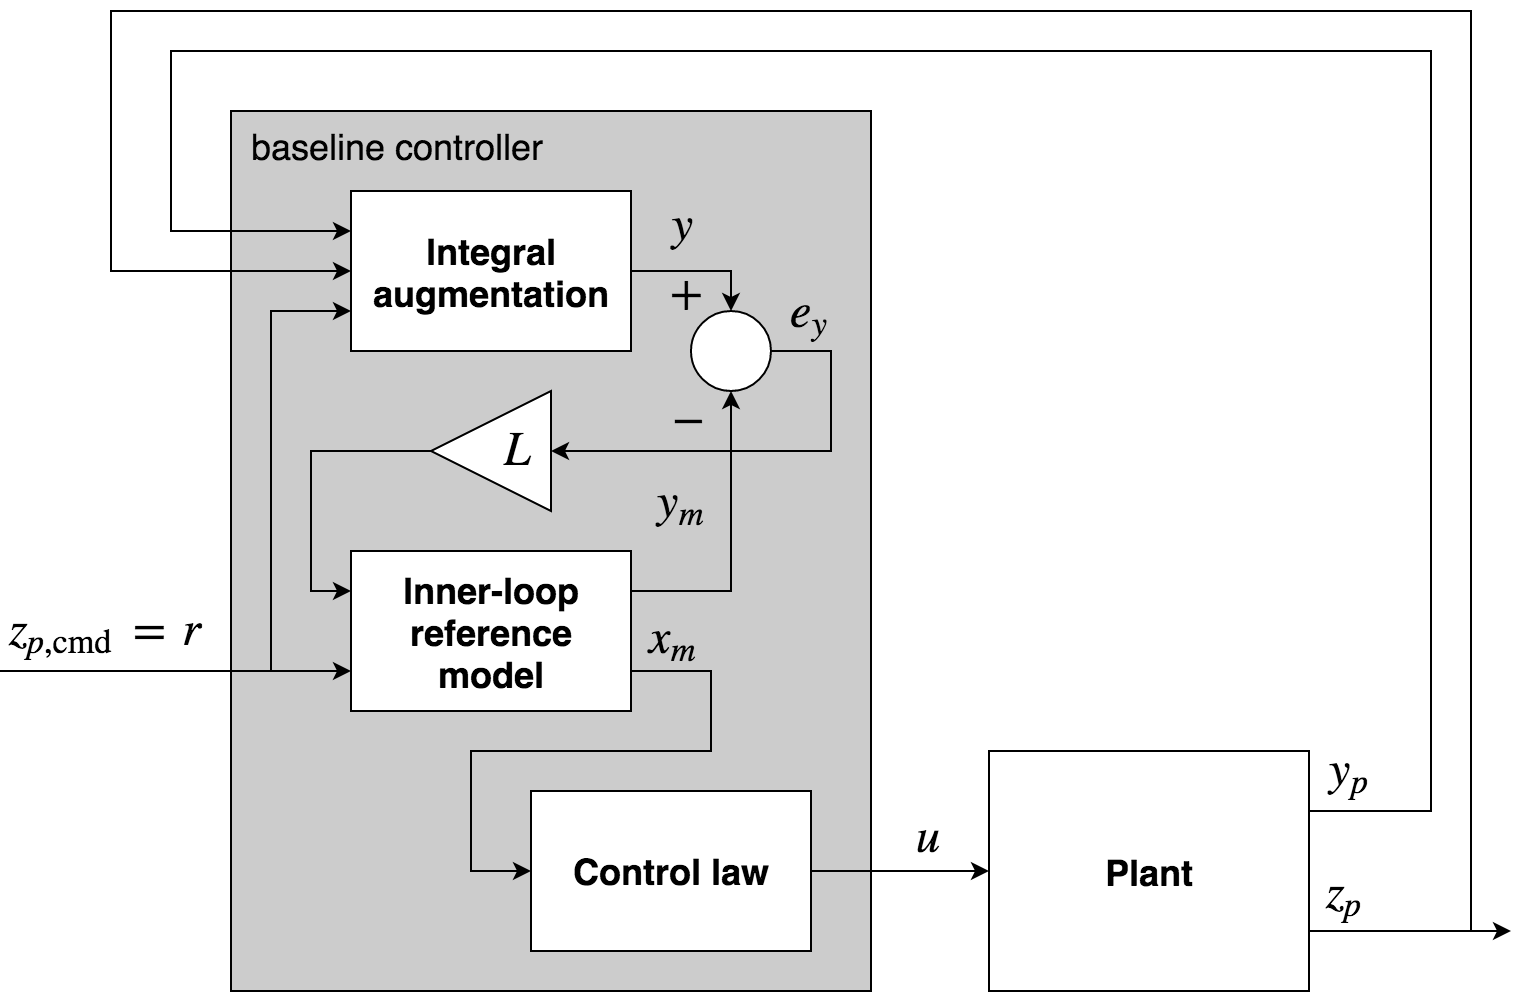
\includegraphics[width=6.5in]{\figurepath/innerLoopBaseline.png}
    \vspace{-0.1in}
    \caption{Inner-loop baseline control block diagram.\label{fig.innerLoopBaseline}}
  \end{center}
\end{figure}

\subsection{Adaptive Controller}

With the baseline controller determined as above, the next step is to design an adaptive controller in the presence of $\Lambda\neq I$ and $\Psi\neq 0$.
Suppose the nominal controller in\ \eqref{eqn.ubl} is augmented with an adaptive element as
\begin{equation}
  \label{eqn.u}
  u(t) = \bigr(K_{x}(t)+\Theta(t)\bigr)^{\top}x_{m}(t)
\end{equation}
where $\Theta(t)$ is to be determined by a suitable update law.
The question is if the introduction of the parameter $\Theta(t)$ as in\ \eqref{eqn.u} is sufficient to accommodate the parametric uncertainties.
For this purpose, a matching condition as described in Remark~\ref{rem.matching}, is introduced below.

\begin{rem-dan}[(Matching condition)]\label{rem.matching}
  The selection of the reference model state matrix as $A_{m}=A+BK_{x}^{\top}$ guarantees the existence of a parameter $\Theta^{*}$ that satisfies the following matching condition.
  \begin{equation*}
    A_{m}=A+B\Psi^{\top}+B\Lambda\bigr(\Theta^{*\top}+K_{x}^{\top}\bigr)
  \end{equation*}
  where $\Theta^{*}$ is given by
  \begin{equation*}
    \Theta^{*\top}=(\Lambda^{-1}-I)K_{x}^{\top}-\Psi^{\top}
  \end{equation*}
\end{rem-dan}

Given a system satisfying Assumption~\ref{ass.uncsystem}, the matching condition in Remark~\ref{rem.matching}, and the proposed control architecture, the reference tracking control problem is reduced to selecting the CRM gain $L$ in\ \eqref{eqn.refmodel} and a suitable adaptive law for updating $\Theta(t)$ in\ \eqref{eqn.u}.

In summary, the problem that is addressed in this chapter is the determination of an adaptive augmented robust baseline output feedback controller as in\ \eqref{eqn.u} to control the plant in\ \eqref{eqn.uncsystem} using the CRM/Observer as in\ \eqref{eqn.refmodel}.
This in turn necessitates finding an adaptive law for adjusting $\Theta$ in\ \eqref{eqn.u} and the observer gain $L$ in\ \eqref{eqn.refmodel}.
The main tools used for determining the adaptive controller were provided in Appendix~\ref{app.preliminaries} and involve the Kalman-Yakubovich\ \cite{narendra.stable.2005} and matrix elimination lemmas\ \cite{boyd.lmibook.1994}, which help reduce the problem of finding $L$ to a state feedback problem of a related lower order subsystem.
The complete adaptive control design and the corresponding stability result are presented in Section~\ref{sec.adaptivecontroldesign}.

\section{Adaptive Control Design}\label{sec.adaptivecontroldesign}

In this section the process for selecting the CRM gain $L$ in\ \eqref{eqn.refmodel} and the update law for $\Theta(t)$ in\ \eqref{eqn.u} is provided.
To accomplish the goal of reference tracking an approach which focuses on the error between the closed-loop plant and the reference model states, as opposed to each of these trajectories individually, is taken.
Thus, the goal of reference tracking can be ensured by appropriately selecting the update law to drive this state error to zero.
Similarly, consider the error between the parameter $\Theta(t)$ in\ \eqref{eqn.u} and $\Theta^{*}$ in Remark~\ref{rem.matching}.
The resulting state tracking error and parameter error, respectively, can be defined as
\begin{align*}
  e_{x}(t) &= x(t) - x_{m}(t) \\
  \widetilde{\Theta}(t) &= \Theta(t) - \Theta^{*}
\end{align*}
The problem of finding an adaptive law for $\Theta(t)$ that guarantees stability depends on the relationship between the two errors above.
This relation, denoted as \textit{error model}, in turn provides cues for determining the adaptive law.
In the problem under consideration, the underlying error model can be described as
\begin{equation}
  \label{eqn.errordynamics1}
  \begin{split}
    \dot{e}_{x}(t) &= (A+LC+B\Psi^{\top})e_{x}(t) + B\Lambda\widetilde{\Theta}^{\top}x_{m}(t) + B_{\text{cmd}}\bigr(z_{p,\text{cmd}}(t) - r(t)\bigr) \\
    e_{y}(t) &= Ce_{x}(t) \\
  \end{split}
\end{equation}
where $e_{y}(t)$ is the measured output error.
Furthermore, select the reference model input $r(t)$ as
\begin{equation}
  \label{eqn.zcmd1}
  r(t) = z_{p,\text{cmd}}(t)
\end{equation}
which is typical in adaptive control and further simplifies the error dynamics in\ \eqref{eqn.errordynamics1} to
\begin{equation}
  \label{eqn.errordynamics2}
  \begin{split}
    \dot{e}_{x}(t) &= \bigr(A+LC+B\Psi^{\top}\bigr)e_{x}(t) + B\Lambda\widetilde{\Theta}^{\top}(t)x_{m}(t) \\
    e_{y}(t) &= Ce_{x}(t) \\
  \end{split}
\end{equation}
As mentioned earlier, the problem of finding a stabilizing adaptive controller is equivalent to finding an $L$ and an adaptive law for adjusting $\widetilde{\Theta}(t)$ in\ \eqref{eqn.errordynamics2}.
Determining a stable adaptive law for an error model as in\ \eqref{eqn.errordynamics2} relies on properties of an underlying transfer function that is SPR\ \cite{narendra.stable.2005}, which in turn enables the use of  Lemma 1 in Appendix~\ref{app.preliminaries}.
However, the definition of SPR is restricted to square transfer functions.
As such, for these properties to be applicable to the error model in\ \eqref{eqn.errordynamics2}, a suitable static postcompensator $S_1\in\mathbb{R}^{m\times p}$ has to be chosen such that
\begin{equation*}
  S_{1}C(sI-A-LC-B\Psi^{\top})^{-1}B \in\mathbb{R}_{p}^{m\times m}(s)
\end{equation*}
where $\mathbb{R}_{p}(s)$ denotes the ring of \textit{proper} rational transfer functions with coefficients in $\mathbb{R}$.
That is the underlying transfer matrix is square, and therefore can be evaluated in terms of SPR properties.
It is therefore necessary to introduce a synthetic output error $e_{s}(t)$ as
\begin{equation}
  \label{eqn.syntheticoutputerror}
  e_{s}(t) = S_{1}Ce_{x}(t)
\end{equation}
Using the synthetic output error in\ \label{eqn.syntheticoutputerror} in place of the output error, the underlying error model in\ \eqref{eqn.errordynamics2} is modified as
\begin{equation}
  \label{eqn.uncerrdyn}
  \begin{split}
    \dot{e}_{x}(t) &= \bigr(A+LC+B\Psi^{\top}\bigr)e_{x}(t) + B\Lambda\widetilde{\Theta}^{\top}(t)x_{m}(t) \\
    e_{s}(t) &= S_{1}Ce_{x}(t)
  \end{split}
\end{equation}
Thus, the design of an output feedback adaptive controller is reduced to selecting matrices $S_{1}\in\mathbb{R}^{m\times p}$ and $L\in\mathbb{R}^{n\times p}$ such that the error dynamics in\ \eqref{eqn.uncerrdyn} are SPR.\@

In Section~\ref{sec.findingS1andL} a procedure to construct $S_{1}$ and $L$ is provided.
This procedure requires $S_{1}$ to be solved as a generalized inverse based on the matrices of $(A,B,C,0)$ in\ \eqref{eqn.uncsystem} alone.
$L$ is found by satisfying Lemma~\ref{lem.KY} (Kalman-Yakubovich), the solution of which is reduced to a state-feedback problem of a lower-order plant subsystem which ultimately leads to a feasible LMI which is solved numerically to obtain $L$.

\subsection{Finding $S_{1}$ and $L$}\label{sec.findingS1andL}

In this section a method for selecting $S_{1}$ and $L$ which ensure the system in\ \eqref{eqn.uncerrdyn} is SPR, is provided.
The conditions from Lemma~\ref{lem.KY} to ensure $(A+LC+B\Psi^{\top},B,S_{1}C)$ is SPR are given by
\begin{align}
  \label{eqn.lyapal}
  (A+LC+B\Psi^{\top})^{\top}P_{x}+P_{x}(A+LC+B\Psi^{\top}) &< 0 \\
  \label{eqn.S1CB}
  P_{x}B &= (S_{1}C)^{\top}
\end{align}
where, by the corollary to Lemma~\ref{lem.KY} in Appendix~\ref{app.preliminaries}, a $P_{x}$ exists which satisfies\ \eqref{eqn.S1CB} if and only if $S_{1}CB=(S_{1}CB)^{\top}$.

\subsubsection{Finding $S_{1}$}

The matrix $S_{1}$ satisfying\ \eqref{eqn.S1CB} can be computed as a generalized left inverse of $CB$ as
\begin{equation}
  \label{eqn.S1}
  S_{1}=\bigr((CB)^{\top}CB\bigr)^{-1}(CB)^{\top}
\end{equation}
Note that this choice of $S_{1}$ is not unique.
An alternative choice for $S_{1}$ is
\begin{equation}
  \label{eqn.S1alternative}
  S_{1} = B^{\top}C^{\top}K_{s}
\end{equation}
where $K_{s}=K_{s}^{\top}\in\mathbb{R}^{p\times p}$.

% TODO@dpwiese - use \texorpdfstring{$L$}{L}
\subsubsection{Finding $L$}\label{subsection.obtainX}

The annihilator matrices $B^{\perp}$ and $C^{\top\perp}$ in Appendix~\ref{app.preliminaries} are not unique.
In the following subsection the notation $N$ and $M$ is used to represent particular annihilators that satisfy
\begin{equation}
  \label{eqn.NB0CM0}
  NB=0
  \qquad
  CM=0
\end{equation}
as well a few additional desired properties.
That is, $N$ represents a particular $B^{\perp\top}$ and $M$ a particular $C^{\top\perp}$.
Given arbitrary annihilators $B^{\perp}$ and $C^{\top\perp}$ a constructive process for obtaining $N$ and $M$ is provided, and these matrices are then used to find $L$.
The inequality\ \eqref{eqn.lyapal} is satisfied if the following inequality is satisfied
\begin{equation}
  \label{eqn.lyapalQ}
  (A+LC)^{\top}P_{x}+P_{x}(A+LC)+Q_{x}<0
\end{equation}
for
\begin{equation}
  \label{eqn.WBTP}
  \Psi B^{\top}P_{x}+P_{x}B\Psi^{\top}<Q_{x}
\end{equation}
Using\ \eqref{eqn.S1CB}, the inequality\ \eqref{eqn.WBTP} can be written as
\begin{equation}
  \label{eqn.WS1C}
  \Psi S_{1}C+(\Psi S_{1}C)^{\top}<Q_{x}
\end{equation}
Note that $Q_{x}$ satisfying\ \eqref{eqn.WS1C} is independent of $P_{x}$.
Using Lemma~\ref{lem.elimination} in Appendix~\ref{app.preliminaries}, an $L$ exists which satisfies\ \eqref{eqn.lyapalQ} if and only if a $P_{x}$ exists which satisfies
\begin{equation}
  \label{eqn.MAPPAM}
  M^{\top}(A^{\top}P_{x}+P_{x}A)M<-M^{\top}Q_{x}M
\end{equation}
Using\ \eqref{eqn.Psolutions}, $P_{x}$ is given by
\begin{equation}
  \label{eqn.Px}
  P_{x} = (S_{1}C)^{\top}(S_{1}CB)^{-\top}S_{1}C+N^{\top}XN
\end{equation}
Substituting the expression for $P_{x}$ from\ \eqref{eqn.Px} into the inequality\eqref{eqn.MAPPAM} the following is obtained
\begin{equation}
  \label{eqn.NAMlyap}
  (NAM)^{\top}XNM+(NM)^{\top}X(NAM)<-M^{\top}Q_{x}M
\end{equation}
Thus, the problem of finding an SPR $L$ which satisfies the inequality\ \eqref{eqn.lyapal} is now reduced to finding the matrix $X$ satisfying the inequality\ \eqref{eqn.NAMlyap}.
An $X$ satisfying\ \eqref{eqn.NAMlyap} specifies a $P_{x}$ as given in\ \eqref{eqn.Px} that reduces\ \eqref{eqn.lyapal} to a feasible LMI in $L$.
This LMI can then be easily solved using any widely available numerical LMI solver to obtain $L$.

Reference\ \cite{huang.designspr.1999} gave the inequality\ \eqref{eqn.NAMlyap} for a square system, suggesting that $X$ be obtained by solving this LMI numerically.
However, it was shown in Reference\ \cite{kouvaritakis.part1.1976} that for a square system, the eigenvalues of $NAM$ in\ \eqref{eqn.NAMlyap} are the transmission zeros of the system and the annihilators $N$ and $M$ in\ \eqref{eqn.NAMlyap} can be always be selected such that $NM=I$.
Given a square system with only stable transmission zeros, this selection reduces\ \eqref{eqn.NAMlyap} to a Lyapunov equation where the matrix $NAM$ is stable, and the existence of $X>0$ satisfying this inequality is guaranteed\ \cite{barkana.comments.2004}.
Thus, when the system $(A,B,C,0)$ in\ \eqref{eqn.uncsystem} is square, the inequality\ \eqref{eqn.NAMlyap} can be solved to obtain $X$, and $P_{x}$ can be computed using\ \eqref{eqn.Px}.
The inequality\ \eqref{eqn.lyapal} can then be solved for $L$.
For a non-square systems the matrix $NAM$ is not square, and so determining $X>0$ satisfying\ \eqref{eqn.NAMlyap} requires additional steps.

\paragraph{Determining a Similarity Transform}
A similarity transform $\Xi$ that will allow annihilator matrices $N$ and $M$ in\ \eqref{eqn.NAMlyap} to be computed given arbitrary annihilators $B^{\perp}$ and $C^{\top\perp}$ is now defined.
Defining $\Xi$ as
\begin{equation}
  \label{eqn.Xi}
  \Xi=
  \begin{bmatrix}
    B & F & C^{\top\perp}
  \end{bmatrix}
\end{equation}
it is always possible to choose $F\in\mathbb{R}^{n\times(p-m)}$ so that $\Xi$ is invertible and
\begin{equation}
  \label{eqn.XiSatisfies}
  \begin{split}
    C\Xi&=
    \begin{bmatrix}
      \bar{C} & 0_{p\times(n-p)}
    \end{bmatrix} \\
    \Xi^{-1}B&=
    \begin{bmatrix}
      I_{m\times m} & 0_{m\times(n-m)}
    \end{bmatrix}^{\top}
  \end{split}
\end{equation}
where $\bar{C}\in\mathbb{R}^{p\times p}$\ \cite{owens.invariant.1977}.
Because of the structure of $B$ and $C$ arising from the integral augmentation and the assumption that $CB$ is full rank, the matrix $F$ in\ \eqref{eqn.Xi} will always have a structure
\begin{equation}
  \label{eqn.F1}
  F =
  \begin{bmatrix}
    0_{n_{p}\times p-m} \\
    F_{1}
  \end{bmatrix}
\end{equation}
where $F_{1}\in\mathbb{R}^{n_{ep}\times p-m}$.
The inverse of $\Xi$ is given by
\begin{equation}
  \label{eqn.Xiinv}
  \Xi^{-1}=
  \begin{bmatrix}
    R \\
    N_{1} \\
    N_{2}
  \end{bmatrix}
\end{equation}
where $R\in\mathbb{R}^{m\times n}$, $N_{1}\in\mathbb{R}^{(p-m)\times n}$ and $N_{2}\in\mathbb{R}^{(n-p)\times n}$.
Given the matrix $\Xi$ in\ \eqref{eqn.Xi}, its inverse $\Xi^{-1}$ must obviously satisfy
\begin{equation}
  \label{eqn.xixi}
  \Xi^{-1}\Xi=
  \begin{bmatrix}
    R \\
    N_{1} \\
    N_{2}
  \end{bmatrix}
  \begin{bmatrix}
    B & F & C^{\top\perp}
  \end{bmatrix}
  =
  \begin{bmatrix}
    RB & RF & RC^{\top\perp} \\
    N_{1}B & N_{1}F & N_{1}C^{\top\perp} \\
    N_{2}B & N_{2}F & N_{2}C^{\top\perp} \\
  \end{bmatrix}
  =
  \begin{bmatrix}
    I & 0 & 0 \\
    0 & I & 0 \\
    0 & 0 & I \\
  \end{bmatrix}
  =
  I
\end{equation}
where the matrix $F$, and thus $\Xi$ and therefore $\Xi^{-1}$ are yet to be determined.
From this it can be seen that
\begin{equation}
  \label{N2B0N2F0N2CTperpI}
  N_{2}B = 0_{(n-p)\times m}
  \qquad
  N_{2}F=0_{(n-p)\times(p-m)}
  \qquad
  N_{2}C^{\top\perp}=I_{(n-p)\times(n-p)}
\end{equation}
Note that by Assumption~\ref{ass.uncsystem}\ref{ass.rank} the matrix $CB$ is full rank, implying that none of the columns of $B$ lie in the nullspace of $C$.
Thus the columns of $\left[ B \; C^{\top\perp} \right]$ are linearly independent.
The columns of $F$ which ensure\ \eqref{eqn.Xi} is invertible lie in $\text{null}(B^{\top})\cap\text{range}(C^{\top})$.
Define
\begin{equation}
  \label{eqn.Abar}
  \begin{split}
    \bar{A}
    &=
    \Xi^{-1}A\Xi=
    \begin{bmatrix}
      R \\
      N_{1} \\
      N_{2}
    \end{bmatrix}
    A
    \begin{bmatrix}
      B & F & C^{\top\perp}
    \end{bmatrix}
    =
    \begin{bmatrix}
      RAB & RAF & RAC^{\top\perp} \\
      N_{1}AB & N_{1}AF & N_{1}AC^{\top\perp} \\
      N_{2}AB & N_{2}AF & N_{2}AC^{\top\perp} \\
    \end{bmatrix} \\
    &=
    \left[
    \begin{array}{c|c} % chktex 44
      \bar{A}_{11} & \bar{A}_{12} \\
      \hline % chktex 44
      \bar{A}_{21} & \bar{A}_{22} \\
      \hline % chktex 44
      \bar{A}_{31} & \bar{A}_{32}
    \end{array}\right] \\
  \end{split}
\end{equation}
where $\bar{A}_{11}\in\mathbb{R}^{m\times p}$, $\bar{A}_{12}\in\mathbb{R}^{m\times(n-p)}$, $\bar{A}_{21}\in\mathbb{R}^{(p-m)\times p}$, $\bar{A}_{22}\in\mathbb{R}^{(p-m)\times(n-p)}$, $\bar{A}_{31}\in\mathbb{R}^{(n-p)\times p}$, and $\bar{A}_{32}\in\mathbb{R}^{(n-p)\times(n-p)}$ are given by
\begin{equation}
  \label{eqn.AbarComponents}
  \begin{aligned}
    \bar{A}_{11}
    &=
    \begin{bmatrix}
      RAB & RAF
    \end{bmatrix}
    \qquad
    &
    \bar{A}_{12}
    &=
    RAC^{\top\perp} \\
    \bar{A}_{21}
    &=
    \begin{bmatrix}
      N_{1}AB & N_{1}AF
    \end{bmatrix}
    &
    \bar{A}_{22}
    &=
    N_{1}AC^{\top\perp} \\
    \bar{A}_{31}
    &=
    \begin{bmatrix}
      N_{2}AB & N_{2}AF
    \end{bmatrix}
    &
    \bar{A}_{32}
    &=
    N_{2}AC^{\top\perp}
  \end{aligned}
\end{equation}
Using\ \eqref{eqn.XiSatisfies} define the following transformed eliminators $N_{0}$ and $M_{0}$ which satisfy $N_{0}\Xi^{-1}B=0_{(n-m)\times m}$ and $C\Xi M_{0}=0_{p\times(n-p)}$ as
\begin{align}
  \label{eqn.N0}
  N_{0}&=
  \begin{bmatrix}
    0_{(n-m)\times m} & I_{(n-m)\times(n-m)}
  \end{bmatrix} \\
  \label{eqn.M0}
  M_{0}&=
  \begin{bmatrix}
    0_{(n-p)\times p} & I_{(n-p)\times(n-p)}
  \end{bmatrix}^{\top}
\end{align}
Note that these choices are not unique.
Define
\begin{align}
  \label{eqn.N}
  N&=N_{0}\Xi^{-1} \\
  \label{eqn.M}
  M&=\Xi M_{0}
\end{align}
Note that with the selection of $M_{0}$ in\ \eqref{eqn.M0} and with $\Xi$ in\ \eqref{eqn.Xi} that $M=C^{\top\perp}$.
The matrix $NM$ is given by
\begin{equation}
  \label{eqn.NM}
  NM=
  \begin{bmatrix}
    0_{(n-p)\times(p-m)} & I_{(n-p)\times(n-p)}
  \end{bmatrix}^{\top}
\end{equation}
With this choice of $\Xi$ and using the form of $\bar{A}$ from\ \eqref{eqn.Abar}, the matrix $NAM$ can be expressed as
\begin{equation}
  \label{eqn.NAM}
  \begin{split}
    NAM &=
    N_{0}\Xi^{-1}A\Xi M_{0} =
    N_{0}\bar{A}M_{0} \\
    &=
    \begin{bmatrix}
      0_{(n-m)\times m} & I_{(n-m)\times(n-m)}
    \end{bmatrix}
    \left[
    \begin{array}{c|c} % chktex 44
      \bar{A}_{11} & \bar{A}_{12} \\
      \hline % chktex 44
      \bar{A}_{21} & \bar{A}_{22} \\
      \hline % chktex 44
      \bar{A}_{31} & \bar{A}_{32}
    \end{array}\right]
    \begin{bmatrix}
      0_{p\times(n-p)} \\ I_{(n-p)\times(n-p)}
    \end{bmatrix} =
    \begin{bmatrix}
      \bar{A}_{22} \\
      \bar{A}_{32}
    \end{bmatrix} \\
  \end{split}
\end{equation}
Note that with the choice of $NM$ satisfying\ \eqref{eqn.NM}, $X$ in\ \eqref{eqn.NAMlyap} can be partitioned as
\begin{equation}
  \label{eqn.Xpartition}
  X=
  \begin{bmatrix}
    X_{11} & X_{12} \\
    X_{12}^{\top} & X_{22}
  \end{bmatrix}
\end{equation}
where $X_{11}\in\mathbb{R}^{(p-m)\times(p-m)}$, $X_{22}\in\mathbb{R}^{(n-p)\times(n-p)}$ and $X_{12}\in\mathbb{R}^{(p-m)\times(n-p)}$.
Furthermore, $X_{12}$ must be selected such that $X_{12}^{\top}N_{1}B_{\text{cmd}}$ is full rank.

\begin{prop-dan}
  Given the matrix $X$ in\ \eqref{eqn.Xpartition} if $X_{22}>0$ then $X>0$ if and only if $X_{11}-X_{12}X_{22}^{-1}X_{12}^{\top}>0$.
  This is the Schur Complement of $X_{22}$.
\end{prop-dan}

\begin{rem-dan}\label{rem.X12FullRank}
  The requirement that $X_{12}$ be selected such that $X_{12}^{\top}N_{1}B_{\text{cmd}}$ is full rank has no impact on the ability to complete the stable inner-loop control design.
  That is, the matrix $X_{12}$ can be selected such that $X_{12}=0$ and still achieve a stable inner-loop controller, although the selection of $X_{12}$ would have an effect on the numerical values of the gains, and hence the underlying baseline controller margins.
  However, the requirement that $X_{12}^{\top}N_{1}B_{\text{cmd}}$ be full rank is needed for the design of the outer-loop controller presented in Chapter~\ref{ch.outerLoop}.
\end{rem-dan}

\begin{lem-dan}
  The requirement that $X_{12}^{\top}N_{1}B_{\text{cmd}}$ is full rank is equivalent to $M^{\top}N^{\top}XNB_{\text{cmd}}$ being full rank.
\end{lem-dan}

\begin{proof-dan}
  Using the expression for $N$ given in\ \eqref{eqn.N}, the matrix $M^{\top}N^{\top}XNB_{\text{cmd}}$ can be written as
  \begin{equation}
    \label{eqn.MtNtXNBcmd}
    M^{\top}N^{\top}XNB_{\text{cmd}}
    =
    M^{\top}(N_{0}\Xi^{-1})^{\top}XN_{0}\Xi^{-1}B_{\text{cmd}}
  \end{equation}
  with $\Xi^{-1}$ given by\ \eqref{eqn.Xiinv}, and $N_{0}$ given by\ \eqref{eqn.N0}, Eq.\ \eqref{eqn.MtNtXNBcmd} can be expressed
  \begin{equation}
    \label{eqn.MtNtXNBcmd2}
    M^{\top}N^{\top}XNB_{\text{cmd}}
    =
    M^{\top}
    \begin{bmatrix}
      R^{\top} & N_{1}^{\top} & N_{2}^{\top}
    \end{bmatrix}
    \begin{bmatrix}
      0 \\
      I
    \end{bmatrix}
    X
    \begin{bmatrix}
      0 & I
    \end{bmatrix}
    \begin{bmatrix}
      R \\
      N_{1} \\
      N_{2}
    \end{bmatrix}
    B_{\text{cmd}}
  \end{equation}
  Multiplying the terms in\ \eqref{eqn.MtNtXNBcmd2} together gives
  \begin{equation*}
    \begin{split}
      M^{\top}N^{\top}XNB_{\text{cmd}}
      &=
      M^{\top}
      \begin{bmatrix}
        R^{\top} & N_{1}^{\top} & N_{2}^{\top}
      \end{bmatrix}
      \begin{bmatrix}
        0 & 0 \\
        0 & X
      \end{bmatrix}
      \begin{bmatrix}
        R \\
        N_{1} \\
        N_{2}
      \end{bmatrix}
      B_{\text{cmd}} \\
      &=
      M^{\top}
      \begin{bmatrix}
        N_{1}^{\top} & N_{2}^{\top}
      \end{bmatrix}
      X
      \begin{bmatrix}
        N_{1} \\
        N_{2}
      \end{bmatrix}
      B_{\text{cmd}}
    \end{split}
  \end{equation*}
  Using the fact that $M^{\top}N_{1}^{\top}=0$ and $M^{\top}N_{2}^{\top}=I$ from\ \eqref{eqn.xixi}, allows this expression to be written and further simplified as follows
  \begin{equation*}
    \begin{split}
      M^{\top}N^{\top}XNB_{\text{cmd}}
      &=
      M^{\top}
      \begin{bmatrix}
        N_{1}^{\top} & N_{2}^{\top}
      \end{bmatrix}
      \begin{bmatrix}
        X_{11} & X_{12} \\
        X_{12}^{\top} & X_{22}
      \end{bmatrix}
      \begin{bmatrix}
        N_{1} \\
        N_{2}
      \end{bmatrix}
      B_{\text{cmd}} \\
      &=
      \begin{bmatrix}
        0 & I
      \end{bmatrix}
      \begin{bmatrix}
        X_{11} & X_{12} \\
        X_{12}^{\top} & X_{22}
      \end{bmatrix}
      \begin{bmatrix}
        N_{1} \\
        N_{2}
      \end{bmatrix}
      B_{\text{cmd}} \\
      &=
      \begin{bmatrix}
        X_{12}^{\top} & X_{22}
      \end{bmatrix}
      \begin{bmatrix}
        N_{1} \\
        N_{2}
      \end{bmatrix}
      B_{\text{cmd}} \\
      &= X_{12}^{\top}N_{1}B_{\text{cmd}} + X_{22}N_{2}B_{\text{cmd}} \\
    \end{split}
  \end{equation*}
  Based on the structure of $B_{\text{cmd}}$ as being in the same space spanned by $F$ in\ \eqref{eqn.F1}, and the requirement in\ \eqref{N2B0N2F0N2CTperpI} that $N_{2}F=0$, it follows that $N_{2}B_{\text{cmd}}=0$, simplifying the above expression as desired.
\end{proof-dan}

Evaluating $XNM$ in\ \eqref{eqn.NAMlyap} using $X$ from\ \eqref{eqn.Xpartition} and $NM$ from\ \eqref{eqn.NM} gives
\begin{equation*}
  XNM=
  \begin{bmatrix}
    X_{12} \\
    X_{22}
  \end{bmatrix}
\end{equation*}
With $NAM$ given by\ \eqref{eqn.NAM}, equation\ \eqref{eqn.NAMlyap} is equivalent to the following
\begin{equation*}
  \begin{bmatrix}
    \bar{A}_{22}^{\top} & \bar{A}_{32}^{\top}
  \end{bmatrix}
  \begin{bmatrix}
    X_{12} \\
    X_{22}
  \end{bmatrix}
  +
  \begin{bmatrix}
    X_{12}^{\top} & X_{22}^{\top}
  \end{bmatrix}
  \begin{bmatrix}
    \bar{A}_{22} \\
    \bar{A}_{32}
  \end{bmatrix}
  <-M^{\top}Q_{x}M
\end{equation*}
which can be written as
\begin{equation*}
  \bar{A}_{22}^{\top}X_{12}
  + X_{12}^{\top}\bar{A}_{22}^{\top}
  + \bar{A}_{32}^{\top}X_{22}
  + X_{22}\bar{A}_{32}
  < -M^{\top}Q_{x}M
\end{equation*}
or alternatively as
\begin{equation}
  \label{eqn.anInnerLoopLyapEq}
  \bar{A}_{32}^{\top}X_{22}
  + X_{22}\bar{A}_{32}
  <
  - M^{\top}Q_{x}M
  - \bar{A}_{22}^{\top}X_{12}
  - X_{12}^{\top}\bar{A}_{22}^{\top}
\end{equation}
Eq.\ \eqref{eqn.anInnerLoopLyapEq} is recognized as a Lyapunov equation
\begin{equation}
  \label{eqn.lyapX22}
  \bar{A}_{32}^{\top}X_{22}+X_{22}\bar{A}_{32}
  =
  - \bar{Q}_{x}
\end{equation}
where $\bar{Q}_{x}$ is selected such that
\begin{equation}
  \label{eqn.Qbar}
  0
  <
  M^{\top}Q_{x}M + \bar{A}_{22}^{\top}X_{12} + X_{12}^{\top}\bar{A}_{22}^{\top}
  <
  \bar{Q}_{x}
\end{equation}
Furthermore, the matrix $F$ which defines $\Xi$ in\ \eqref{eqn.Xi} must be selected such that $\bar{A}_{32}$, given in\ \eqref{eqn.AbarComponents}, is Hurwitz, thus allowing $X_{22}$ to be obtained as the solution to\ \eqref{eqn.lyapX22}.
$X_{11}>0$ can then be selected arbitrarily to specify $X$.
Recall from\ \eqref{eqn.xixi} that $N_{2}$ has to satisfy $N_{2}B=0$, $N_{2}C^{\top\perp}=I$, and $N_{2}F=0$.
To satisfy the first of these two conditions, it is apparent that $N_{2}$ lies in the nullspace of $B^{\top}$ and so $N_{2}$ has the form
\begin{equation}
  \label{eqn.N2}
  N_{2}=KB^{\perp\top}
\end{equation}
where $K\in\mathbb{R}^{(n-p)\times(n-m)}$.
With the choice of $N_{2}$ as in\ \eqref{eqn.N2} the second condition from\ \eqref{eqn.xixi} requires that $K$ satisfies $KB^{\perp\top}C^{\top\perp} = I$, where such a $K$ takes the columns of $B^{\perp}$ which are spanned by the columns of $C^{\top\perp}$.
The columns of $K^{\perp}B^{\perp}$ where $K^{\perp}$ satisfies $KK^{\perp}=0$ thus lie in $\text{null}(B^{\top})\cap\text{range}(C^{\top})$, and so selecting $F$ as
\begin{equation}
  \label{eqn.FF}
  F = B^{\perp}K^{\perp}
\end{equation}
ensures that\ \eqref{eqn.Xi} is invertible.
With the choice of $N_{2}$ as in\ \eqref{eqn.N2} the matrix $\bar{A}_{32}$ can then be expressed as
\begin{equation*}
  \bar{A}_{32}=KB^{\perp\top}AC^{\top\perp}
\end{equation*}
The remaining requirements described above are stated as: find $K\in\mathbb{R}^{(n-p)\times(n-m)}$ such that
\begin{align}
  \label{eqn.Kgeninv}
  KB^{\perp\top}C^{\top\perp}&=I_{(n-p)\times(n-p)} \\
  \label{eqn.eigK}
  \bar{A}_{32}=KB^{\perp\top}AC^{\top\perp}&\qquad\text{is Hurwitz}
\end{align}

\paragraph{An Equivalent State Feedback Problem}

The control design process continues by showing how the selection of $K$ satisfying\ \eqref{eqn.Kgeninv} and\ \eqref{eqn.eigK}, can be found by solving a state feedback problem.
The requirement in\ \eqref{eqn.Kgeninv} is that $K$ is a left inverse of the tall matrix $B^{\perp\top}C^{\top\perp}$.
This matrix has full rank by Assumption~\ref{ass.uncsystem}\ref{ass.rank}.
The generalized inverse of a tall matrix $T\in\mathbb{R}^{(n-m)\times(n-p)}$ with full rank is given by
\begin{equation*}
  T^{-}=T^{\dagger}+U(I_{(n-m)\times(n-m)}-TT^{\dagger})
\end{equation*}
where $U\in\mathbb{R}^{(n-p)\times(n-m)}$ is arbitrary and $\dagger$ is the Moore-Penrose pseudo inverse.
This gives a form of all $K$ satisfying\ \eqref{eqn.Kgeninv} as
\begin{equation*}
  K=(B^{\perp\top}C^{\top\perp})^{\dagger}+U\left(I_{(n-m)\times(n-m)}-(B^{\perp\top}C^{\top\perp})(B^{\perp\top}C^{\top\perp})^{\dagger}\right)
\end{equation*}
This can be simplified as
\begin{empheq}[]{alignat=3}
  K&=(B^{\perp\top}C^{\top\perp})^{\dagger}+U\left(I_{(n-m)\times(n-m)}-J\right)\label{eqn.K} \\
  J&=(B^{\perp\top}C^{\top\perp})(B^{\perp\top}C^{\top\perp})^{\dagger}\label{eqn.J}
\end{empheq}
where $J\in\mathbb{R}^{(n-m)\times(n-m)}$ is a rank $n-p$ matrix.
Thus $\bar{A}_{32}$ is given by
\begin{equation*}
  \bar{A}_{32}=
  \biggr[(B^{\perp\top}C^{\top\perp})^{\dagger}+U\left(I_{(n-m)\times(n-m)}-J\right)\biggr]B^{\perp\top}AC^{\top\perp}
\end{equation*}
which can be written
\begin{equation}
  \label{eqn.Abar32GUH}
  \bar{A}_{32}=
  G+UH
\end{equation}
where $G\in\mathbb{R}^{(n-p)\times(n-p)}$ and $H\in\mathbb{R}^{(n-m)\times(n-p)}$ are given by
\begin{empheq}[]{alignat=3}
  G&=(B^{\perp\top}C^{\top\perp})^{\dagger}B^{\perp\top}AC^{\top\perp}\label{eqn.G} \\
  H&=\bigr(I_{(n-m)\times(n-m)}-J\bigr)B^{\perp\top}AC^{\top\perp}\label{eqn.H}
\end{empheq}
Selecting $U$ such that $\bar{A}_{32}$ is Hurwitz is possible in general if $(G^{\top},H^{\top})$ is controllable.
The uncontrollable modes of $(G^{\top},H^{\top})$ correspond to the transmission zeros of $(A,B,C,0)$\ \cite{kouvaritakis.part2.1976}.
If the system has any unstable zeros, no $U$ can be found such that $\bar{A}_{32}$ is Hurwitz.
If the system has stable transmission zeros, $(G^{\top},H^{\top})$ is stabilizable, and $U$ can be selected to stabilize the remaining modes.
If the system has no transmission zeros, $(G^{\top},H^{\top})$ is controllable, and $U$ can be picked to make the poles of $\bar{A}_{32}$ arbitrarily.
By Assumption~\ref{ass.uncsystem}\ref{ass.tzero} $(A,B,C,0)$ has no unstable transmission zeros, so $(G^{\top},H^{\top})$ will be at least stabilizable.
With $U$ computed using the desired state-space technique, $\bar{A}_{32}$ is determined as in\ \eqref{eqn.Abar32GUH}.
$K$ can then be solved for from\ \eqref{eqn.K} and\ \eqref{eqn.J}, $N_{2}$ computed using\ \eqref{eqn.N2} and $F$ using\ \eqref{eqn.FF}.
With this $F$, the matrix $\Xi$ is completely specified, and $N$ can be solved for from\ \eqref{eqn.N} and $M$ given by $M=C^{\top\perp}$.
Finally,\ \eqref{eqn.lyapX22} must be solved to obtain $X_{22}$, which requires the specification of $Q_{x}>0$.
The following paragraph and theorem provide a method to select an appropriate $Q_{x}$.

\paragraph{Solving the LMI to Obtain $L$}

All that remains to solve the LMI in\ \eqref{eqn.lyapalQ} for $L$ is to specify $P_{x}$ as given by\ \eqref{eqn.Px} and $Q$ satisfying\ \eqref{eqn.WS1C}.
Therefore it is necessary to choose an appropriate $Q$ which guarantees the feasibility of the LMI in\ \eqref{eqn.lyapalQ} by satisfying\ \eqref{eqn.WS1C}, as given by the following theorem.

\begin{thm-dan}
  If $Q_{x}$ is chosen as
  \begin{equation}
    \label{eqn.Q}
    Q_{x}=2\Psi_{\rm{\max}}\|C_{s}\|_{2}I_{n\times n}
  \end{equation}
  where $C_{s}=S_{1}C$ and $\Psi_{\rm{\max}}$ is defined as in Assumption~\ref{ass.plant}\ref{ass.p.unc}-(\ref{ass.p.unc.wp}), then\ \eqref{eqn.WS1C} holds.
\end{thm-dan}

\begin{proof-dan}
  Using $C_{s}=S_{1}C$ the inequality\ \eqref{eqn.WS1C} can be written
  \begin{equation*}
    \Psi C_{s}+(\Psi C_{s})^{\top}<Q_{x}
  \end{equation*}
  Using $\Psi C_{s}\leq\|\Psi C_{s}\|_{2}I\leq\|\Psi\|_{2}\|C_{s}\|_{2}I<\Psi_{\rm{\max}}\|C_{s}\|_{2}I$ the matrix $Q_{x}$ in\ \eqref{eqn.Q} satisfies\ \eqref{eqn.WS1C}.
\end{proof-dan}

With $Q_{x}$ picked as in\ \eqref{eqn.Q}, $\bar{A}_{32}$ made stable by selection of $U$ in\ \eqref{eqn.Abar32GUH}, and $\bar{Q}_{x}$ selected satisfying\ \eqref{eqn.Qbar}, the Lyapunov equation in\ \eqref{eqn.lyapX22} can be solved to obtain $X_{22}$.
This procedure guarantees the feasibility of the LMI in\ \eqref{eqn.lyapalQ} which can be solved numerically with any widely available solver.
This procedure is summarized in the following subsection.

\subsection{Summary of the Design Procedure for $S_{1}$ and $L$}\label{sec.designprocedure}

Section~\ref{sec.findingS1andL} provided a procedure to determine $S_{1}$ and $L$ for the system $(A,B,C,0)$ satisfying Assumption~\ref{ass.uncsystem} which render\ \eqref{eqn.uncerrdyn} SPR.\@
This subsection summarizes the overall procedure.
Given known plant matrices $A$, $B$, $B_{\text{cmd}}$, $C$, knowledge of the sign of the uncertainty $\Lambda$ and upper bound $\|\Psi\|_{2}\leq\Psi_{\text{max}}$ in\ \eqref{eqn.uncsystem}, reference model in\ \eqref{eqn.refmodel}, and control law in\ \eqref{eqn.u}, the following steps provide a procedure to determine $S_{1}$ and $L$ such that the underlying error dynamics in\ \eqref{eqn.uncerrdyn} are SPR:\@

\begin{enumerate}[1.]
  \setlength{\itemsep}{0pt}
  \item{Solve for $S_{1}$ as in\ \eqref{eqn.S1}.}
  \item{Determine arbitrary annihilators $B^{\perp}$ and $C^{\top\perp}$ such that $B^{\top}B^{\perp}=0$ and $CC^{\top\perp}=0$.}
  \item{\label{step.U}Calculate matrices $G$ and $H$ using\ \eqref{eqn.J},\ \eqref{eqn.G}, and\ \eqref{eqn.H} and then solve for $U$ such that $\bar{A}_{32}$ in\ \eqref{eqn.Abar32GUH} is Hurwitz.}
  \item{Compute $K$ using\ \eqref{eqn.K}, $F$ using\ \eqref{eqn.FF}, and $N_{2}$ using\ \eqref{eqn.N2}.}
  \item{Define $N_{0}$ as in\ \eqref{eqn.N0}. Calculate $N=N_{0}\Xi^{-1}$ and set $M=C^{\top\perp}$.}
  \item{Pick $X_{12}$ such that $X_{12}^{\top}N_{1}B_{\text{cmd}}$ is full rank.}
  \item{\label{step.X22} Select $Q_{x}$ as in\ \eqref{eqn.Q} and $\bar{Q}_{x}$ satisfying\ \eqref{eqn.Qbar} and solve\ \eqref{eqn.lyapX22} to obtain $X_{22}$}
  \item{\label{step.X11} Select $X_{11}$ satisfying $X_{11}>X_{12}X_{22}^{-1}X_{12}^{\top}$ and assemble $X$ as in\ \eqref{eqn.Xpartition}}
  \item{Solve for $P_{x}$ as in\ \eqref{eqn.Px}.}
  \item{Solve the LMI in\ \eqref{eqn.lyapalQ} to obtain $L$}
\end{enumerate}

\begin{rem-dan}\label{rem.pmgeqnp}
  In the case where $p-m\geq n-p$, the matrix $H$ in\ \eqref{eqn.Abar32GUH} is a matrix of full column rank and so $H^{\dagger}H=I_{(n-p)\times(n-p)}$.
  This provides the freedom in selecting $U$ to not only make $\bar{A}_{32}$ stable, but to select it to be any stable matrix.
  This allows us to select $X_{22}>0$ arbitrarily, and then solve for $\bar{A}_{32}^{*}$ as the solution to the Lyapunov equation $\bar{A}_{32}^{*\top}X_{22}+X_{22}\bar{A}_{32}^{*}=-M^{\top}QM$.
  Then $U$ can be picked in step~\ref{step.U} as
  \begin{equation}
    \label{eqn.Uremark}
    U=\bigr(\bar{A}_{32}^{*}-G\bigr)H^{\dagger}
  \end{equation}
\end{rem-dan}

\begin{figure}[H]
  \begin{center}
    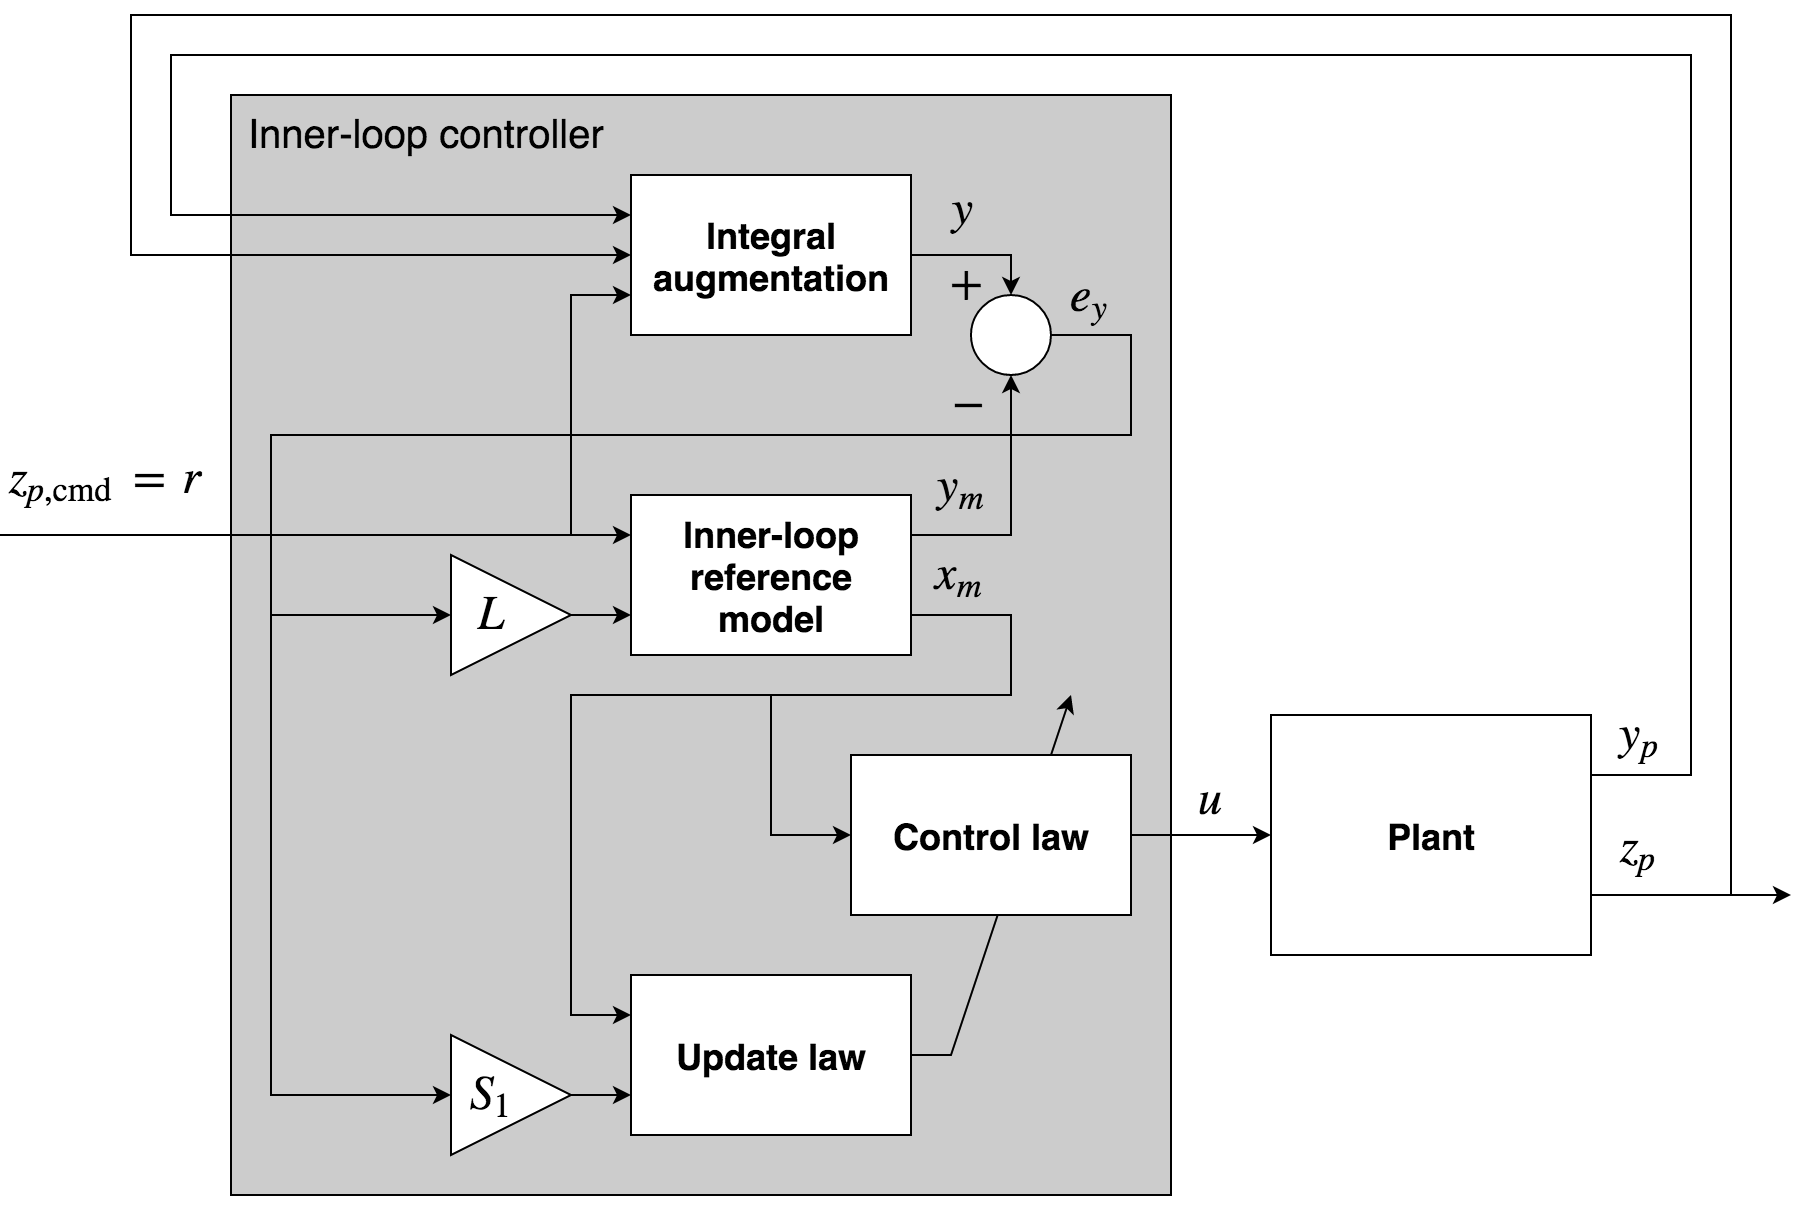
\includegraphics[width=6.5in]{\figurepath/innerLoop2.png}
    \vspace{-0.1in}
    \caption{Inner-loop adaptive control block diagram.\label{fig.innerLoop2}}
  \end{center}
\end{figure}

\begin{rem-dan}
  The calculation of $L$ should conclude with the verification that $A+LC+BK_{x}^{\top}$ is Hurwitz.
  While this is not a theoretical requirement, for practical implementation on systems such as the one presented in the numerical example in Chapter~\ref{ch.applicationHypersonic}, this requirement is enforced to ensure the reference model in\ \eqref{eqn.refmodel} is stable.
\end{rem-dan}

\subsection{Adaptive Law and Stability Proof}\label{sec.adaptivelaw}

Using the closed-loop reference model defined in\ \eqref{eqn.refmodel} with $L$ selected as described in Section~\ref{sec.findingS1andL}, the following update law is proposed:
\begin{equation}
  \label{eqn.updatelaw}
  \dot{\widetilde{\Theta}}(t) = -\Gamma x_{m}(t)\bigr(S_{1}e_{y}(t)\bigr)^{\top}\text{sgn}(\Lambda)
\end{equation}
where $S_{1}$ is chosen using\ \eqref{eqn.S1}.
The closed-loop system is represented using the block diagram shown in Figure~\ref{fig.innerLoop2}.
Alternatively, the inner-loop controller can be represented using the block diagram shown in Figure~\ref{fig.innerLoop3}.

\begin{figure}[H]
  \begin{center}
    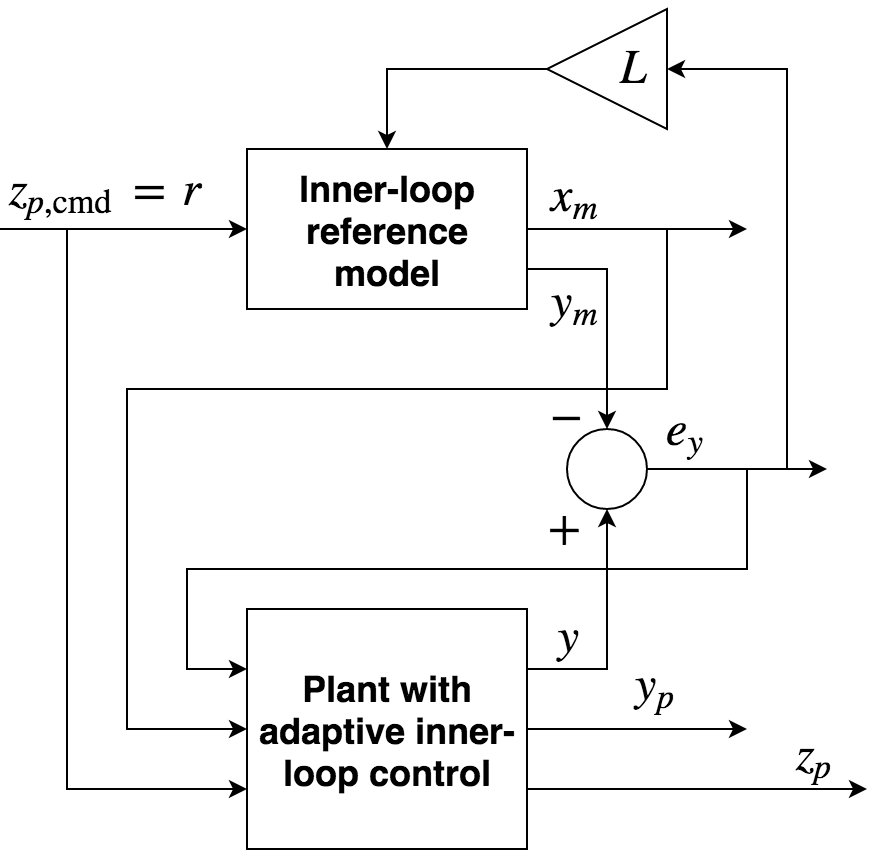
\includegraphics[width=3.5in]{\figurepath/innerLoop3.png}
    \vspace{-0.1in}
    \caption{Inner-loop control block diagram.\label{fig.innerLoop3}}
  \end{center}
\end{figure}

Global stability of the closed-loop system is guaranteed by the following theorem.

\begin{thm-dan}\label{thm.innerLoopStability}
  Given the uncertain linear system in\ \eqref{eqn.uncsystem} which satisfies Assumption~\ref{ass.uncsystem}, the reference model in\ \eqref{eqn.refmodel} with reference input selected as in\ \eqref{eqn.zcmd1}, control law as in\ \eqref{eqn.u}, and the update law in\ \eqref{eqn.updatelaw} results in global stability, with $\lim_{t\rightarrow\infty}e_{x}(t)=0$.
\end{thm-dan}

\begin{proof-dan}
  With a radially unbounded Lyapunov function candidate
  \begin{equation}
    \label{eqn.lyapfunction}
    V\bigr(e_{x}(t),\widetilde{\Theta}(t)\bigr) = e_{x}^{\top}(t)P_{x}e_{x}(t)+\text{tr}\bigr(|\Lambda|\widetilde{\Theta}^{\top}(t)\Gamma^{-1}\widetilde{\Theta}(t)\bigr)
  \end{equation}
  where the operation $|\cdot|$ takes the absolute value of each entry of the matrix argument, a time-derivative $\dot{V}\bigr(e_{x}(t),\widetilde{\Theta}(t)\bigr)$ is obtained as
  \begin{equation*}
    \dot{V}\bigr(e_{x}(t),\widetilde{\Theta}(t)\bigr) = \dot{e}_{x}^{\top}(t)P_{x}e_{x}(t)+e_{x}^{\top}(t)P_{x}\dot{e}_{x}(t)+\text{tr}\bigr(|\Lambda|\dot{\widetilde{\Theta}}^{\top}(t)\Gamma^{-1}\widetilde{\Theta}(t)\bigr)+\text{tr}\bigr(|\Lambda|\widetilde{\Theta}^{\top}(t)\Gamma^{-1}\dot{\widetilde{\Theta}}(t)\bigr)
  \end{equation*}
  Substituting in the error dynamics from\ \eqref{eqn.uncerrdyn} where $A_{L} = A + LC + B\Psi^{\top}$ the Lyapunov candidate derivative $\dot{V}\bigr(e_{x}(t),\widetilde{\Theta}(t)\bigr)$ is written
  \begin{equation*}
    \begin{split}
      \dot{V}\bigr(e_{x}(t),\widetilde{\Theta}(t)\bigr)
      &=
      \bigr(A_{L}e_{x}(t)+B\Lambda\widetilde{\Theta}^{\top}(t)x_{m}(t)\bigr)^{\top}P_{x}e_{x}(t)+e_{x}^{\top}(t)P_{x}\bigr(A_{L}e_{x}(t)+B\Lambda\widetilde{\Theta}^{\top}(t)x_{m}(t)\bigr) \\
      & \qquad + 2\text{tr}\bigr(|\Lambda|\widetilde{\Theta}^{\top}(t)\Gamma^{-1}\dot{\widetilde{\Theta}}(t)\bigr) \\
      %
      &=
      e_{x}^{\top}(t)A_{L}^{\top}P_{x}e_{x}(t) + e_{x}^{\top}(t)P_{x}A_{L}e_{x}(t)+2e_{x}^{\top}(t)PB\Lambda\widetilde{\Theta}^{\top}(t)x_{m}(t) \\
      & \qquad + 2\text{tr}\bigr(|\Lambda|\widetilde{\Theta}^{\top}(t)\Gamma^{-1}\dot{\widetilde{\Theta}}(t)\bigr) \\
      %
      &=
      e_{x}^{\top}(t)(A_{L}^{\top}P_{x}+P_{x}A_{L})e_{x}(t) + 2e_{x}^{\top}(t)P_{x}B\Lambda\widetilde{\Theta}^{\top}(t)x_{m}(t) \\
      & \qquad + 2\text{tr}\bigr(|\Lambda|\widetilde{\Theta}^{\top}(t)\Gamma^{-1}\dot{\widetilde{\Theta}}(t)\bigr) \\
    \end{split}
  \end{equation*}
  Let $A_{L}^{\top}P+PA_{L}=-Q_{x}<0$ as assured by the selection of $L$ satisfying\ \eqref{eqn.lyapal} giving
  \begin{equation*}
    \dot{V}\bigr(e_{x}(t),\widetilde{\Theta}(t)\bigr)
    =
    -e_{x}^{\top}(t)Q_{x}e_{x}(t) + 2e_{x}^{\top}(t)P_{x}B\Lambda\widetilde{\Theta}^{\top}(t)x_{m}(t)+2\text{tr}\bigr(|\Lambda|\widetilde{\Theta}^{\top}(t)\Gamma^{-1}\dot{\widetilde{\Theta}}(t)\bigr)
  \end{equation*}
  Substituting the update law given in\ \eqref{eqn.updatelaw} results in
  \begin{equation*}
    \begin{split}
      \dot{V}\bigr(e_{x}(t),\widetilde{\Theta}(t)\bigr)
      &=
      -e_{x}^{\top}(t)Q_{x}e_{x}(t) + 2e_{x}^{\top}(t)C^{\top}S_{1}^{\top}\Lambda\widetilde{\Theta}^{\top}(t)x_{m}(t) \\
      & \qquad + 2\text{tr}\bigr(|\Lambda|\widetilde{\Theta}^{\top}(t)\Gamma^{-1}\bigr(-\Gamma x_{m}(t)e_{y}^{\top}(t)S_{1}^{\top}\text{sgn}(\Lambda)\bigr)\bigr) \\
      &=
      -e_{x}^{\top}(t)Q_{x}e_{x}(t) + 2e_{s}^{\top}(t)\Lambda\widetilde{\Theta}^{\top}(t)x_{m}(t) - 2\text{tr}\bigr(|\Lambda|\widetilde{\Theta}^{\top}(t)x_{m}(t)e_{y}^{\top}(t)S_{1}^{\top}\text{sgn}(\Lambda)\bigr) \\
      &=
      -e_{x}^{\top}(t)Q_{x}e_{x}(t) + 2e_{s}^{\top}(t)\Lambda\widetilde{\Theta}^{\top}(t)x_{m}(t) - 2\text{tr}\bigr(e_{s}^{\top}(t)\Lambda\widetilde{\Theta}^{\top}(t)x_{m}(t)\bigr) \\
      &=
      -e_{x}^{\top}(t)Q_{x}e_{x}(t) \\
    \end{split}
  \end{equation*}
  Which implies that $V\bigr(e_{x}(t),\widetilde{\Theta}(t)\bigr)$ is a Lyapunov function.
  Since $V\bigr(e_{x}(t),\widetilde{\Theta}(t)\bigr)\succ0$ and $\dot{V}\bigr(e_{x}(t),\widetilde{\Theta}(t)\bigr)\preceq0$, it follows that $V(t)\leq V(0)<\infty$.
  Thus $V(t)\in\mathcal{L}_{\infty}$ which implies $e_{x}(t), \; \widetilde{\Theta}(t)\in\mathcal{L}_{\infty}$.
  Since $z_{p,\text{cmd}}(t),\;e_{x}(t)\in\mathcal{L}_{\infty}$ and the reference model is stable, $x_{m}(t)\in\mathcal{L}_{\infty}$, which implies that $x(t)\in\mathcal{L}_{\infty}$.
  Furthermore,
  \begin{equation*}
    \int_{0}^{t}\dot{V}(\tau)d\tau=V(t)-V(0)
  \end{equation*}
  and since $V\bigr(e_{x}(t),\widetilde{\Theta}(t)\bigr)$ is non increasing and positive definite, $V(0)-V(t)\leq V(0)$.
  This gives
  \begin{equation*}
    -\int_{0}^{t}\dot{V}(\tau)d\tau\leq V(0)
  \end{equation*}
  Substituting in the expression for
  \begin{equation*}
    \dot{V}\bigr(e_{x}(t),\widetilde{\Theta}(t)\bigr) = -e_{x}^{\top}(t)Q_{x}e_{x}(t)
  \end{equation*}
  gives
  \begin{equation*}
    \int_{0}^{t}e_{x}(\tau)^{\top}Q_{x}e_{x}(\tau)d\tau\leq V(0)
  \end{equation*}
  and in turn that $e_{x}(t)\in\mathcal{L}_{2}$.
  Finally, looking at\ \eqref{eqn.uncerrdyn} with $e_{x}(t), \; \widetilde{\Theta}(t), \;\text{and } x_{m}(t)\in\mathcal{L}_{\infty}$ it follows that $\dot{e}_{x}(t)\in\mathcal{L}_{\infty}$.
  With this, it can be concluded using Barbalat's Lemma\ \cite{narendra.stable.2005} that $\lim_{t\rightarrow\infty}e_{x}(t)=0$.
  Since\ \eqref{eqn.lyapfunction} is radially unbounded stability is global.
\end{proof-dan}

\begin{rem-dan}
  The use of the closed-loop reference model in\ \eqref{eqn.refmodel} in no way compromises stability of the closed-loop system.
  Furthermore, with $e_{x}(t)\rightarrow0$ asymptotically as $t\rightarrow\infty$, the term $L\bigr(y_{m}(t)-y(t)\bigr)$ in\ \eqref{eqn.refmodel} tends to zero asymptotically, which in turn indicates that the output of the closed-loop reference model in\ \eqref{eqn.refmodel} tracks that of an open loop reference model, given by\ \eqref{eqn.refmodel} with $L=0$, asymptotically.
  The transient response of the closed-loop reference model as compared with its open-loop counterpart have been discussed in\ \cite{gibson.acc.2013,gibson.ecc.2013,gibson.ieeeaccess.2013}.
  Bounded reference tracking of $z_{p,\text{cmd}}(t)$ by $z_{p}(t)$ follows from  the stability of the closed-loop system as described in the Corollary~\ref{cor.zpcmdtracking} below.
\end{rem-dan}

\begin{cor-dan}\label{cor.zpcmdtracking}
  The inner-loop regulated output $z_{p}(t)$ tracks the inner-loop reference model regulated output $z_{pm}(t)$ asymptotically.
  Furthermore, for piecewise constant commands $z_{p,\text{cmd}}(t)$, the regulated output $z_{p}(t)$ tracks $z_{p,\text{cmd}}(t)$ asymptotically.
\end{cor-dan}

\begin{proof-dan}
  From $\lim_{t\rightarrow\infty}e_{x}(t)=0$ it follows that $\lim_{t\rightarrow\infty}\bigr(x_{e}(t)-x_{em}(t)\bigr) = 0$ where $x_{e}(t)$ is defined in\ \eqref{eqn.xedot} and $x_{em}(t)$ is defined in\ \eqref{eqn.uncertainssRefModel} as $\dot{x}_{em}(t) = z_{p,\text{cmd}}(t) - z_{pm}(t) + L_{e}\bigr(y_{m}(t)-y(t)\bigr)$.
  With this, the following limit can be written
  \begin{equation*}
    \lim_{t\rightarrow\infty}
    \left(
    \int_{0}^{t} \bigr(z_{p,\text{cmd}}(\tau) - z_{p}(\tau)\bigr) d\tau - \int_{0}^{t} \bigr(z_{p,\text{cmd}} - z_{pm}(\tau) + L_{e}C\bigr(x_{m}(\tau)-x(\tau)\bigr)\bigr) d\tau
    \right) = 0
  \end{equation*}
  simplifying
  \begin{equation}
    \label{eqn.intezp}
    \lim_{t\rightarrow\infty}
    \int_{0}^{t} \bigr(z_{p}(\tau) - z_{pm}(\tau)\bigr) d\tau
    =
    \lim_{t\rightarrow\infty}
    L_{e}C \int_{0}^{t} e_{x}(\tau) d\tau < \infty
  \end{equation}
  where the error $e_{zp}(t)$ is given by
  \begin{equation*}
    e_{zp}(t) = z_{p}(t) - z_{pm}(t)
  \end{equation*}
  Recall now that the goal is to show $\lim_{t\rightarrow\infty}e_{zp}(t)=0$.
  Writing out the expression for $e_{zp}(t)$, it follows that
  \begin{equation*}
    e_{zp}(t) = C_{z}x(t) + D_{pz}\bigr(\Lambda u(t) + \Psi^{\top}x(t)\bigr) - C_{z}x_{m}(t) - D_{pz}u_{\text{bl}}(t)
  \end{equation*}
  with $u(t)$ in\ \eqref{eqn.u} and $u_{\text{bl}}(t)$ in\ \eqref{eqn.ubl} the error $e_{zp}(t)$ can be written as
  \begin{equation}
    \label{eqn.ezp}
    \begin{split}
      e_{zp}(t)
      &=
      C_{z}x(t) + D_{pz}\bigr(\Lambda \bigr(K_{x}+\Theta(t)\bigr)^{\top}x_{m}(t)+\Psi^{\top}x(t)\bigr) - C_{z}x_{m}(t) - D_{pz}K_{x}^{\top}x_{m}(t) \\
      &=
      C_{z}e_{x}(t) + D_{pz}\bigr(\Lambda \bigr(K_{x}+\widetilde{\Theta}(t)+\Theta^{*}\bigr)^{\top}x_{m}(t) + \Psi^{\top}x(t) - K_{x}^{\top}x_{m}(t)\bigr) \\
      &=
      C_{z}e_{x}(t) + D_{pz}\bigr(\Lambda \bigr(K_{x}+\Theta^{*}\bigr)^{\top}x_{m}(t) + \Lambda\widetilde{\Theta}^{\top}x_{m}(t)+\Psi^{\top}x(t) - K_{x}^{\top}x_{m}(t)\bigr) \\
    \end{split}
  \end{equation}
  Taking the time derivative of\ \eqref{eqn.ezp} gives
  \begin{equation}
    \label{eqn.ezpdot}
    \dot{e}_{zp}(t)
    =
    C_{z}\dot{e}_{x}(t) + D_{pz}\bigr(\Lambda\bigr(K_{x}+\Theta^{*}\bigr)^{\top}\dot{x}_{m}(t) + \Lambda(\dot{\widetilde{\Theta}}^{\top}(t)x_{m}(t)+\widetilde{\Theta}^{\top}(t)\dot{x}_{m}(t))+\Psi^{\top}\dot{x}(t) - K_{x}^{\top}\dot{x}_{m}(t)\bigr)
  \end{equation}
  Recall Barbalat's Lemma\ \cite{slotine.appliednonlinear.1991}: If a function $f(t)$ has a finite limit as $t\rightarrow\infty$ and if $\dot{f}(t)$ is uniformly continuous (which is equivalent to $\ddot{f}(t)$ being bounded) then $\lim_{t\rightarrow\infty}\dot{f}(t)=0$.
  For this application, let $f(t)=\int_{0}^{t} e_{zp}(\tau) d\tau$ and $\dot{f}(t)=e_{zp}(t)$ and $\ddot{f}(t)=\dot{e}_{zp}(t)$.
  From\ \eqref{eqn.intezp} the function $f(t)$ has a finite limit as $t\rightarrow\infty$.
  Looking at $\ddot{f}(t)=\dot{e}_{z}(t)$ in\ \eqref{eqn.ezpdot}, all of the arguments are bounded, so $\dot{e}_{zp}(t)$ is bounded.
  Thus $\lim_{t\rightarrow\infty}\dot{f}(t)=0$ which is equivalent to $\lim_{t\rightarrow\infty}e_{zp}(t)=0$ as desired.

  Furthermore, with the embedded integrator, the reference model in\ \eqref{eqn.refmodel}, is a type 1 system with respect to the command input.
  With this, the tracking error tending to zero asymptotically as $\lim_{t\rightarrow\infty}e_{x}(t)=0$, and the reference model input in\ \eqref{eqn.zcmd1}, it follows that $z_{pm}(t)\rightarrow z_{p,\text{cmd}}(t)$ as $t\rightarrow\infty$ for piecewise constant commands $z_{p,\text{cmd}}(t)$.
  From this, it follows that $z_{p}(t)\rightarrow z_{p,\text{cmd}}(t)$ asymptotically as $t\rightarrow\infty$, thus satisfying the control goal as desired.
\end{proof-dan}

\begin{rem-dan}
  Corollary~\ref{cor.zpcmdtracking} provides the expected tracking result, in that asymptotic tracking of an arbitrary bounded command $z_{p,\text{cmd}}(t)$ is not possible.
  For example, if the command is a square wave, the best tracking performance that can be achieved is by enforcing the plant to track a suitably filtered version of the command signal.
  In this way, the reference model is essentially serving as a command pre-filter.
\end{rem-dan}

\begin{rem-dan}
  When compared to the existing CRM based adaptive control approaches\ \cite{lavretsky.output.2010, lavretskywise.book.2013, qu.gnc.2013}, the  CRM based method presented in this thesis offers an approach which is computationally simpler, requiring primarily finding nullspaces of some matrices, as described in the step-by-step procedure in Section~\ref{sec.designprocedure}.
\end{rem-dan}

In the following section the applicability of the CRM based method as compared to the classical MIMO adaptive control method is examined.

\section{Comparison Between CRM Based and Classical MIMO Adaptive Control}\label{sec.AdaptiveComparison}

Given the classical approaches used in the  literature thus far, the obvious question that is raised is how the proposed MIMO controller fares compared to the classical ones.
The first point to note here is that the classical approaches are limited to square plants while the approach proposed here is not.
This is the most obvious advantage of this method.
The next question that arises is a comparison of the two approaches when the underlying plant is square.
This is addressed below.

As a first step, the relevant definitions are provided below:

\begin{defn-dan}[(Markov Parameters)]\cite{antsaklis.linearsystems.2006}\label{defn.markov}
  Given a transfer matrix $G(s)$, the \textit{Markov Parameters} are given by
  \begin{equation*}
    H_{0}=\lim_{s\rightarrow\infty}G(s),
    \qquad
    H_{1}=\lim_{s\rightarrow\infty}s(G(s)-H_{0}),
    \qquad
    H_{2}=\lim_{s\rightarrow\infty}s^{2}(G(s)-H_{0}-H_{1}s^{-1})
  \end{equation*}
  and so forth.
\end{defn-dan}

\begin{thm-dan}\label{thm.markov_realization}
  The set $(A,B,C,D)$ is a realization of $G(s)$ if and only if
  \begin{equation*}
    H_{0}=D
    \qquad
    H_{i}=CA^{i-1}B, \quad i=1,2,\dots
  \end{equation*}
\end{thm-dan}

\begin{proof-dan}
  The proof can be found in Reference\ \cite{antsaklis.linearsystems.2006}.
\end{proof-dan}

\begin{defn-dan}
  \textbf{(Relative Degree One)}\label{defn.relativedegreeone}
  The MIMO system $G(s)$ with realization $(A,B,C,D)$ is said to be Relative Degree One if $H_{0}=0$ and $H_{1}=CB$ is full rank.
\end{defn-dan}

\begin{lem-dan}\label{lem.E}
  Reference\ \cite{narendra.stable.2005}
  Given a square nonsingular strictly proper transfer matrix $W_{p}(s)\in\mathbb{R}_{p}^{m\times m}(s)$, its Hermite form is diagonal if and only if the constant matrix $E(W_{p}(s))$ is nonsingular, where $E$ is calculated as follows.
  Calculate $r_{i}$ as the minimum relative degree in the $i^{\text{th}}$ row of $W_{p}(s)$ and the rows of $E$ are
  \begin{equation}
    \label{eqn.Ei}
    E_{i}=\lim_{s\rightarrow\infty}s^{r_{i}}W_{p,i}(s)
  \end{equation}
  where $W_{p,i}(s)$ corresponds to the $i^{\text{th}}$ row of $W_{p}(s)$.
\end{lem-dan}

\begin{proof-dan}
  The proof can be found in Reference\ \cite{chen.introduction.1970}
\end{proof-dan}

Given $W_{p}(s)\in\mathbb{R}_{p}^{m\times m}(s)$, the assumptions that must be satisfied for a classical adaptive control solution to exist are as follows\ \cite{narendra.stable.2005}.

\begin{customthm}{2} $\;$\label{ass.classical}
  \begin{enumerate}[(\roman{enumi}), ref=\roman{enumi}]
    \itemsep0em
    \item{The high frequency gain matrix $K_{p}$ is of the form $K_{p}=\overline{K}_{p}\Lambda$ where $\overline{K}_{p}$ is known and $\text{sign}(\Lambda)$ is known.\label{ass.kp}}
    \item{The right Hermite normal form $H_{p}(s)$ of $W_{p}(s)$ is known.\label{ass.hermite}}
    \item{An upper bound $\nu$ on the observability index of $W_{p}(s)$ is known.\label{ass.nu}}
    \item{The zeros of $W_{p}(s)$ lie in $\mathbb{C}^{-}$.\label{ass.tzeroWp}}
  \end{enumerate}
\end{customthm}

\begin{thm-dan}\label{thm.CB}
  Given the square plant $W_{p}(s)\in\mathbb{R}_{p}^{m\times m}$ with realization $(A,B,C,0)$, the Hermite form $H_{p}(s)$ of $W_{p}(s)$ is diagonal if $CB$ is full rank.
  Furthermore, the high frequency gain matrix is given by $K_{p}=CB$.
\end{thm-dan}

\begin{proof-dan}
  Theorem~\ref{thm.markov_realization} connects the Markov Parameters of Relative Degree One systems to the realization of $W_{p}(s)$ with $H_{0}=0$ and $H_{1}=CB$.
  With this and Definition~\ref{defn.markov}, $\lim_{s\rightarrow\infty}sW_{p}(s)=CB$ is full rank, and so the minimum relative degree in each row of $W_{p}(s)$ is $r_{i}=1$.
  By Lemma~\ref{lem.E} $E(W_{p}(s))=CB$ and the Hermite form $H_{p}(s)$ of $W_{p}(s)$ is diagonal.
  In Reference\ \cite{narendra.stable.2005} it is shown that $E(W_{p}(s))=K_{p}$.
\end{proof-dan}

Using Definitions~\ref{defn.markov} and~\ref{defn.relativedegreeone} as well as Theorems~\ref{thm.markov_realization} and~\ref{thm.CB}, it is shown in Proposition~\ref{prop.mimoequiv} that the classical and the CRM based MIMO adaptive control solution in this paper are equally applicable when the system in\ \eqref{eqn.xdotpunc} is square.

\begin{prop-dan}\label{prop.mimoequiv}
  Consider the uncertain system in\ \eqref{eqn.xdotpunc} where $\ell=m$ and the plant transfer matrix is given by
  \begin{equation}
    \label{eqn.wpofs}
    W_{p}(s)=C_{p}(sI-A_{p}-B_{p} \Psi_{p}^{\top})^{-1}B_{p}\Lambda
  \end{equation}
  if the plant in\ \eqref{eqn.xdotpunc} satisfies Assumption~\ref{ass.plant}, then the corresponding $W_p(s)$ in\ \eqref{eqn.wpofs} satisfies Assumption~\ref{ass.classical}.
\end{prop-dan}

\begin{proof-dan}
  Assumption~\ref{ass.plant}\ref{ass.p.unc}-(\ref{ass.p.unc.lambda}) and Theorem~\ref{thm.CB} can be shown to imply that the corresponding $K_p$ satisfies Assumption~\ref{ass.classical}(\ref{ass.kp}).
  Assumption~\ref{ass.plant}\ref{ass.p.rank} together with Theorem~\ref{thm.CB} implies that the corresponding Hermite form is diagonal with known entries and is therefore known, which leads to Assumption~\ref{ass.classical}(\ref{ass.hermite}).
  Assumption~\ref{ass.classical}(\ref{ass.nu}) follows from the fact that $n_{p}$ is known.
  Finally Assumption~\ref{ass.plant}\ref{ass.p.tzero} is equivalent to Assumption~\ref{ass.classical}(\ref{ass.tzeroWp}).
\end{proof-dan}

In addition to the main advantage of the proposed method of applicability to non-square plants, the proposed controller is of lower order, requiring only $n$ controller states and $nm$ adjustable parameters, as compared with the classical solution which will introduce $2m\nu$ states and $2m^{2}\nu$ parameters.
This reduces the number of states and parameters necessary by at least two, since $n\leq\nu m$\ \cite{chen.linear.1999}.
Finally the proposed solution is based on a CRM, which has been shown to possess a superior transient performance\ \cite{gibson.aiaacrm.2012,gibson.acc.2013,gibson.ecc.2013,gibson.ieeeaccess.2013}.

It should be noted that of Assumptions~\ref{ass.plant}\ref{ass.p.cont}-\ref{ass.p.unc}, which are required to be satisfied for the proposed controller, the most restrictive one is Assumption~\ref{ass.plant}\ref{ass.p.rank}, which implies that the MIMO system must have Relative Degree One.
In most aerial platforms including hypersonic vehicles, this assumption is easy to satisfy as the relative degree of the transfer functions between the control surface deflections and aircraft angular rates is unity.
Additionally, the structure of the plant as in\ \eqref{eqn.xdotpunc} which has matched uncertainties is also commonly present in flight control applications where much of the plant uncertainty is in the aerodynamic moment coefficients and loss of control effectiveness, which are spanned by the columns of $B$.
It is however required that the uncertainty $\Psi_{p}$ satisfy Assumption~\ref{ass.plant}\ref{ass.p.unc}-(\ref{ass.p.unc.wp}), which is not required in the classical approach.
Note finally that the above comparison between the proposed controller and the classical ones was done for Relative Degree One plants only.
Clearly the classical methods such as those in Reference\ \cite{narendra.stable.2005} are applicable to plants with with larger relative degrees, where the proposed method is not.

\section{Numerical Examples}\label{sec.innerLoopNumericalExample}

\subsection{Example 1: Inverted Pendulum Cart}

Consider the inverted cart-pendulum system as given in Ref.\ \cite{astrom.feedbackintro.2010} and shown in Fig.~\ref{fig.pendulumCart}.

\begin{figure}[H]
  \begin{center}
    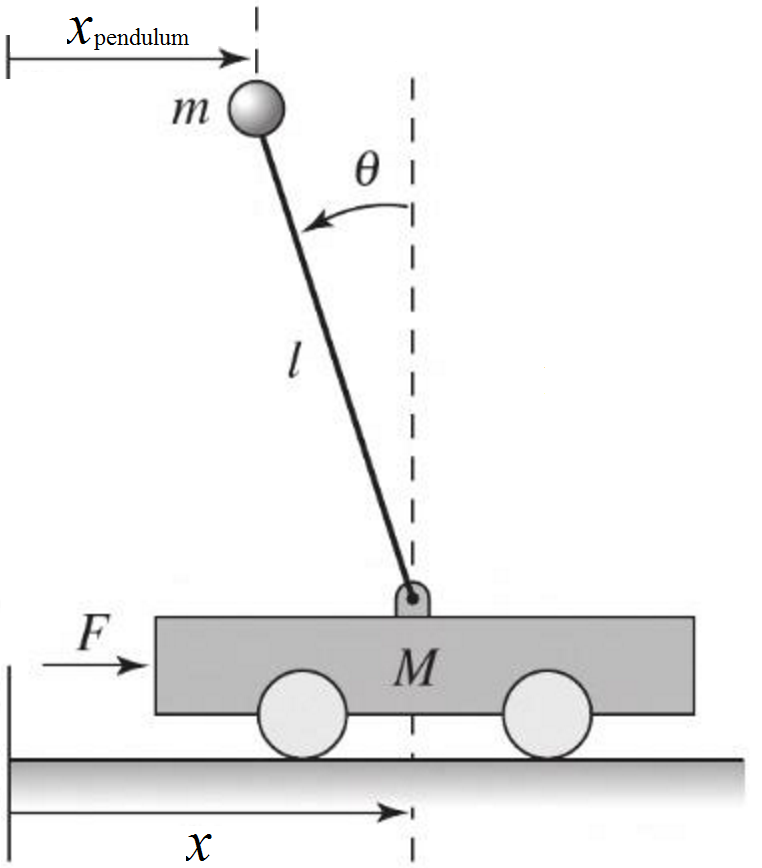
\includegraphics[width=2.8in]{\figurepath/pendulumCart.png}
    \vspace{-0.1in}
    \caption{Inverted pendulum on cart from Ref.\ \cite{astrom.feedbackintro.2010}.\label{fig.pendulumCart}}
  \end{center}
\end{figure}

The linearized equations of motion are given by the following, where $M$ is the mass of the cart, $m$ is the mass of the pendulum, $J$ is the moment of inertia of the pendulum, $l$ is the pendulum length, $c$ and $\gamma$ are coefficients of viscous friction, and $g$ is the acceleration due to gravity.
\begin{equation}
  \label{eqn.pendulumCartWhole}
  \begin{bmatrix}
    \ddot{\theta} \\
    \ddot{x} \\
    \dot{\theta} \\
    \dot{x}
  \end{bmatrix}
  =
  \begin{bmatrix}
    -\frac{\gamma M_{t}}{\mu} & -\frac{cl m}{\mu} & \frac{M_{t}mgl}{\mu} & 0 \\
    -\frac{\gamma J_{t}l m}{\mu} & -\frac{cJ_{t}}{\mu} & \frac{m^{2}g^{2}l}{\mu} & 0 \\
    1 & 0 & 0 & 0 \\
    0 & 1 & 0 & 0 \\
  \end{bmatrix}
  \begin{bmatrix}
    \dot{\theta} \\
    \dot{x} \\
    \theta \\
    x
  \end{bmatrix}
  +
  \begin{bmatrix}
    \frac{l m}{\mu} \\
    \frac{J_{t}}{\mu} \\
    0 \\
    0
  \end{bmatrix}
  F
\end{equation}
where the total mass $M_{t}$ and total moment of inertia $J_{t}$ are given by
\begin{equation*}
  \begin{aligned}
    M_{t} & = M + m \\
    J_{t} &= J + ml^{2}
  \end{aligned}
\end{equation*}
and where $\mu$ is given by
\begin{equation*}
  \mu = M_{t}J_{t} - m^{2}l^{2}
\end{equation*}
Considering uncertainty in the coefficients of viscous friction, this system is represented by Eq.\ \eqref{eqn.wholeSystemUncertain}.
Partitioning\ \eqref{eqn.pendulumCartWhole} as described in Chapter~\ref{ch.Introduction}, the inner-loop dynamics in the form of\ \eqref{eqn.innerLoopDynamicsUncertain} and outer-loop dynamics as in\ \eqref{eqn.outerLoopDynamics} are obtained.
The following numerical values were selected
\begin{equation}
  \label{eqn.pendulumNumericalValues}
  \begin{aligned}
    m &= 1 \text{~kg} \\
    M &= 1 \text{~kg} \\
    l &= 1 \text{~m} \\
    \gamma &= 1 \text{~Ns/m} \\
    c &= 1 \text{~Ns/m} \\
    g &= 9.8 \text{~m/s}^2
  \end{aligned}
\end{equation}
The inner-loop control goal is to stabilize the system using a single velocity measurement.
The velocity of the cart $\dot{x}$ is selected, with this output serving as both the measured and regulated outputs, leading to the following inner-loop dynamics
\begin{equation}
  \label{eqn.pendulumCartInnerLoop}
  \begin{split}
    \begin{bmatrix}
      \ddot{\theta} \\
      \ddot{x}
    \end{bmatrix}
    &=
    \begin{bmatrix}
      -\frac{\gamma M_{t}}{\mu} & -\frac{cl m}{\mu} \\
      -\frac{\gamma J_{t}l m}{\mu} & -\frac{cJ_{t}}{\mu}
    \end{bmatrix}
    \begin{bmatrix}
      \dot{\theta} \\
      \dot{x}
    \end{bmatrix}
    +
    \begin{bmatrix}
      \frac{l m}{\mu} \\
      \frac{J_{t}}{\mu}
    \end{bmatrix}
    F \\
    \dot{x}
    &=
    \begin{bmatrix}
      0 & 1
    \end{bmatrix}
    \begin{bmatrix}
      \dot{\theta} \\
      \dot{x}
    \end{bmatrix}
  \end{split}
\end{equation}
Using the numerical values in\ \eqref{eqn.pendulumNumericalValues}, the system in\ \eqref{eqn.pendulumCartInnerLoop} is given by
\begin{equation*}
  \begin{split}
    \begin{bmatrix}
      \ddot{\theta} \\
      \ddot{x}
    \end{bmatrix}
    &=
    \begin{bmatrix}
      -2 & -1 \\
      -1 & -1
    \end{bmatrix}
    \begin{bmatrix}
      \dot{\theta} \\
      \dot{x}
    \end{bmatrix}
    +
    \begin{bmatrix}
      1 \\
      1
    \end{bmatrix}
    F \\
    \dot{x}
    &=
    \begin{bmatrix}
      0 & 1
    \end{bmatrix}
    \begin{bmatrix}
      \dot{\theta} \\
      \dot{x}
    \end{bmatrix}
  \end{split}
\end{equation*}
The following uncertainty was selected, which is equivalent to the damping coefficient $c=0$, thus making the uncertain system marginally stable, as well as having a reduction in the input to 65\% the nominal control force applied to the cart.
\begin{equation*}
  \begin{split}
    \Psi_{p}
    &=
    \begin{bmatrix}
      0 & 1
    \end{bmatrix}^{\top} \\
    \Lambda
    &=
    0.65
  \end{split}
\end{equation*}
The following weighting matrices were used to design the LQR inner-loop baseline controller
\begin{equation*}
  \begin{split}
    Q_{\text{lqr}}
    &=
    \text{diag}\bigr(
    \begin{bmatrix}
    0 & 0 & 1
    \end{bmatrix}\bigr) \\
    R_{\text{lqr}}
    &=
    10{-6}
  \end{split}
\end{equation*}
The following upper-bound on the uncertainty was used
\begin{equation*}
  \Psi_{\text{max}} = 10
\end{equation*}
resulting in $X$ in\ \eqref{eqn.Px} given by
\begin{equation*}
  X =
  \begin{bmatrix}
    1.1 & 1 \\
    1 & 10
  \end{bmatrix}
\end{equation*}
This inner-loop adaptive controller was then implemented in a simulation of the pendulum model, resulting in the response shown in Fig.~\ref{fig.innerLoopPendulumCart}.
In the following simulations, the simulation begins with the baseline controller applied to the nominal system.
At $t=10$ seconds uncertainty is introduced, while still using only the baseline controller.
At $t=30$ seconds adaptive controller is turned on.
In these simulations, it is important to first note that the oscillations observed in the baseline response are due to the coupling of the kinematics, in this case the pendulum angle, into the dynamics.
While it is often assumed, as described above, that the term associated with this coupling, $B_{gd}$, is negligible, it will still have an impact on the closed-loop performance, except in cases when it is identically zero.
While the nominal response does contain oscillations, they are damped, and steady-state tracking of the piecewise constant cart velocity command is achieved.
When uncertainty is introduced, the oscillations become much larger, and begin to diverge, indicating the uncertainty has made the closed-loop system very lightly damped, and slightly unstable.
The adaptive controller, when turned on, quickly recovers the nominal performance.

\newpage
\begin{figure}[H]
  \hspace{-0.25in}
  \noindent\makebox[7.0in]{%
  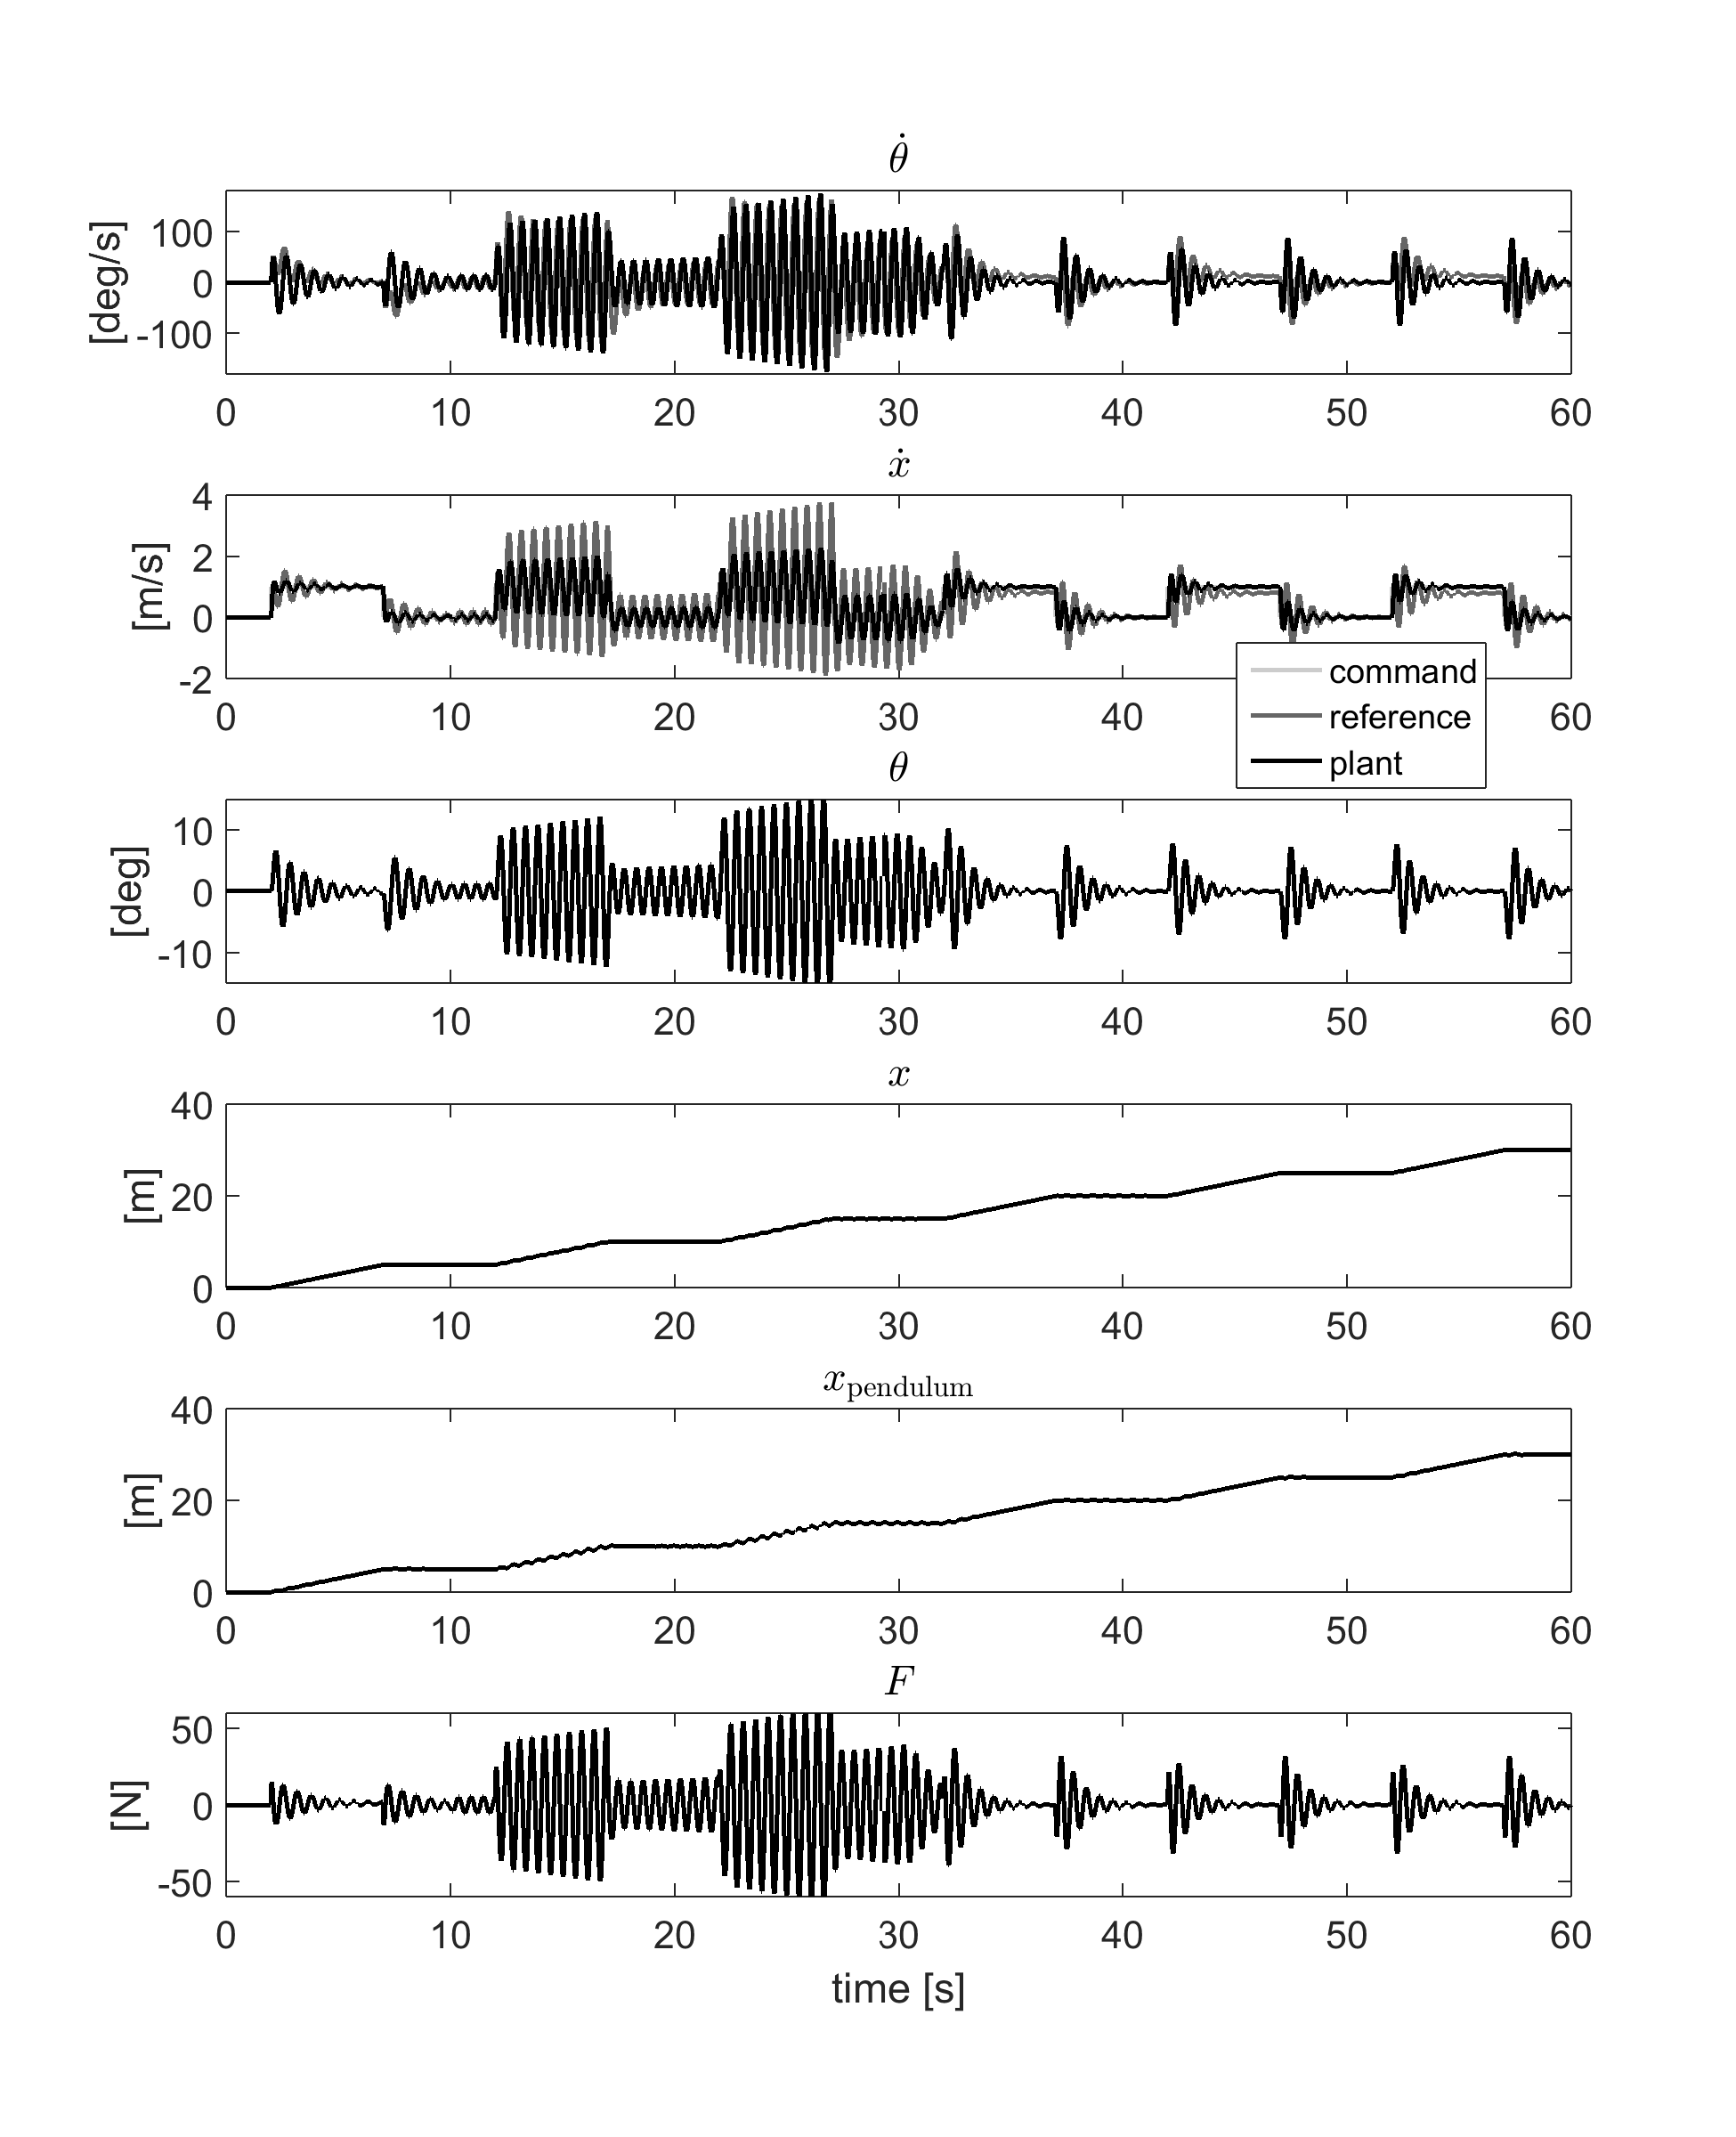
\includegraphics[width=7.0in]{\figurepath/innerLoopPendulumCart.png}}
  \vspace{-0.95in}
  \caption{Time response of pendulum cart with inner-loop controller.\label{fig.innerLoopPendulumCart}}
\end{figure}

\subsection{Example 2: Longitudinal Dynamics of a Transport Aircraft}

For this example, consider the longitudinal dynamics of a transport aircraft, in this case a 747--100.
\begin{figure}[H]
  \begin{center}
    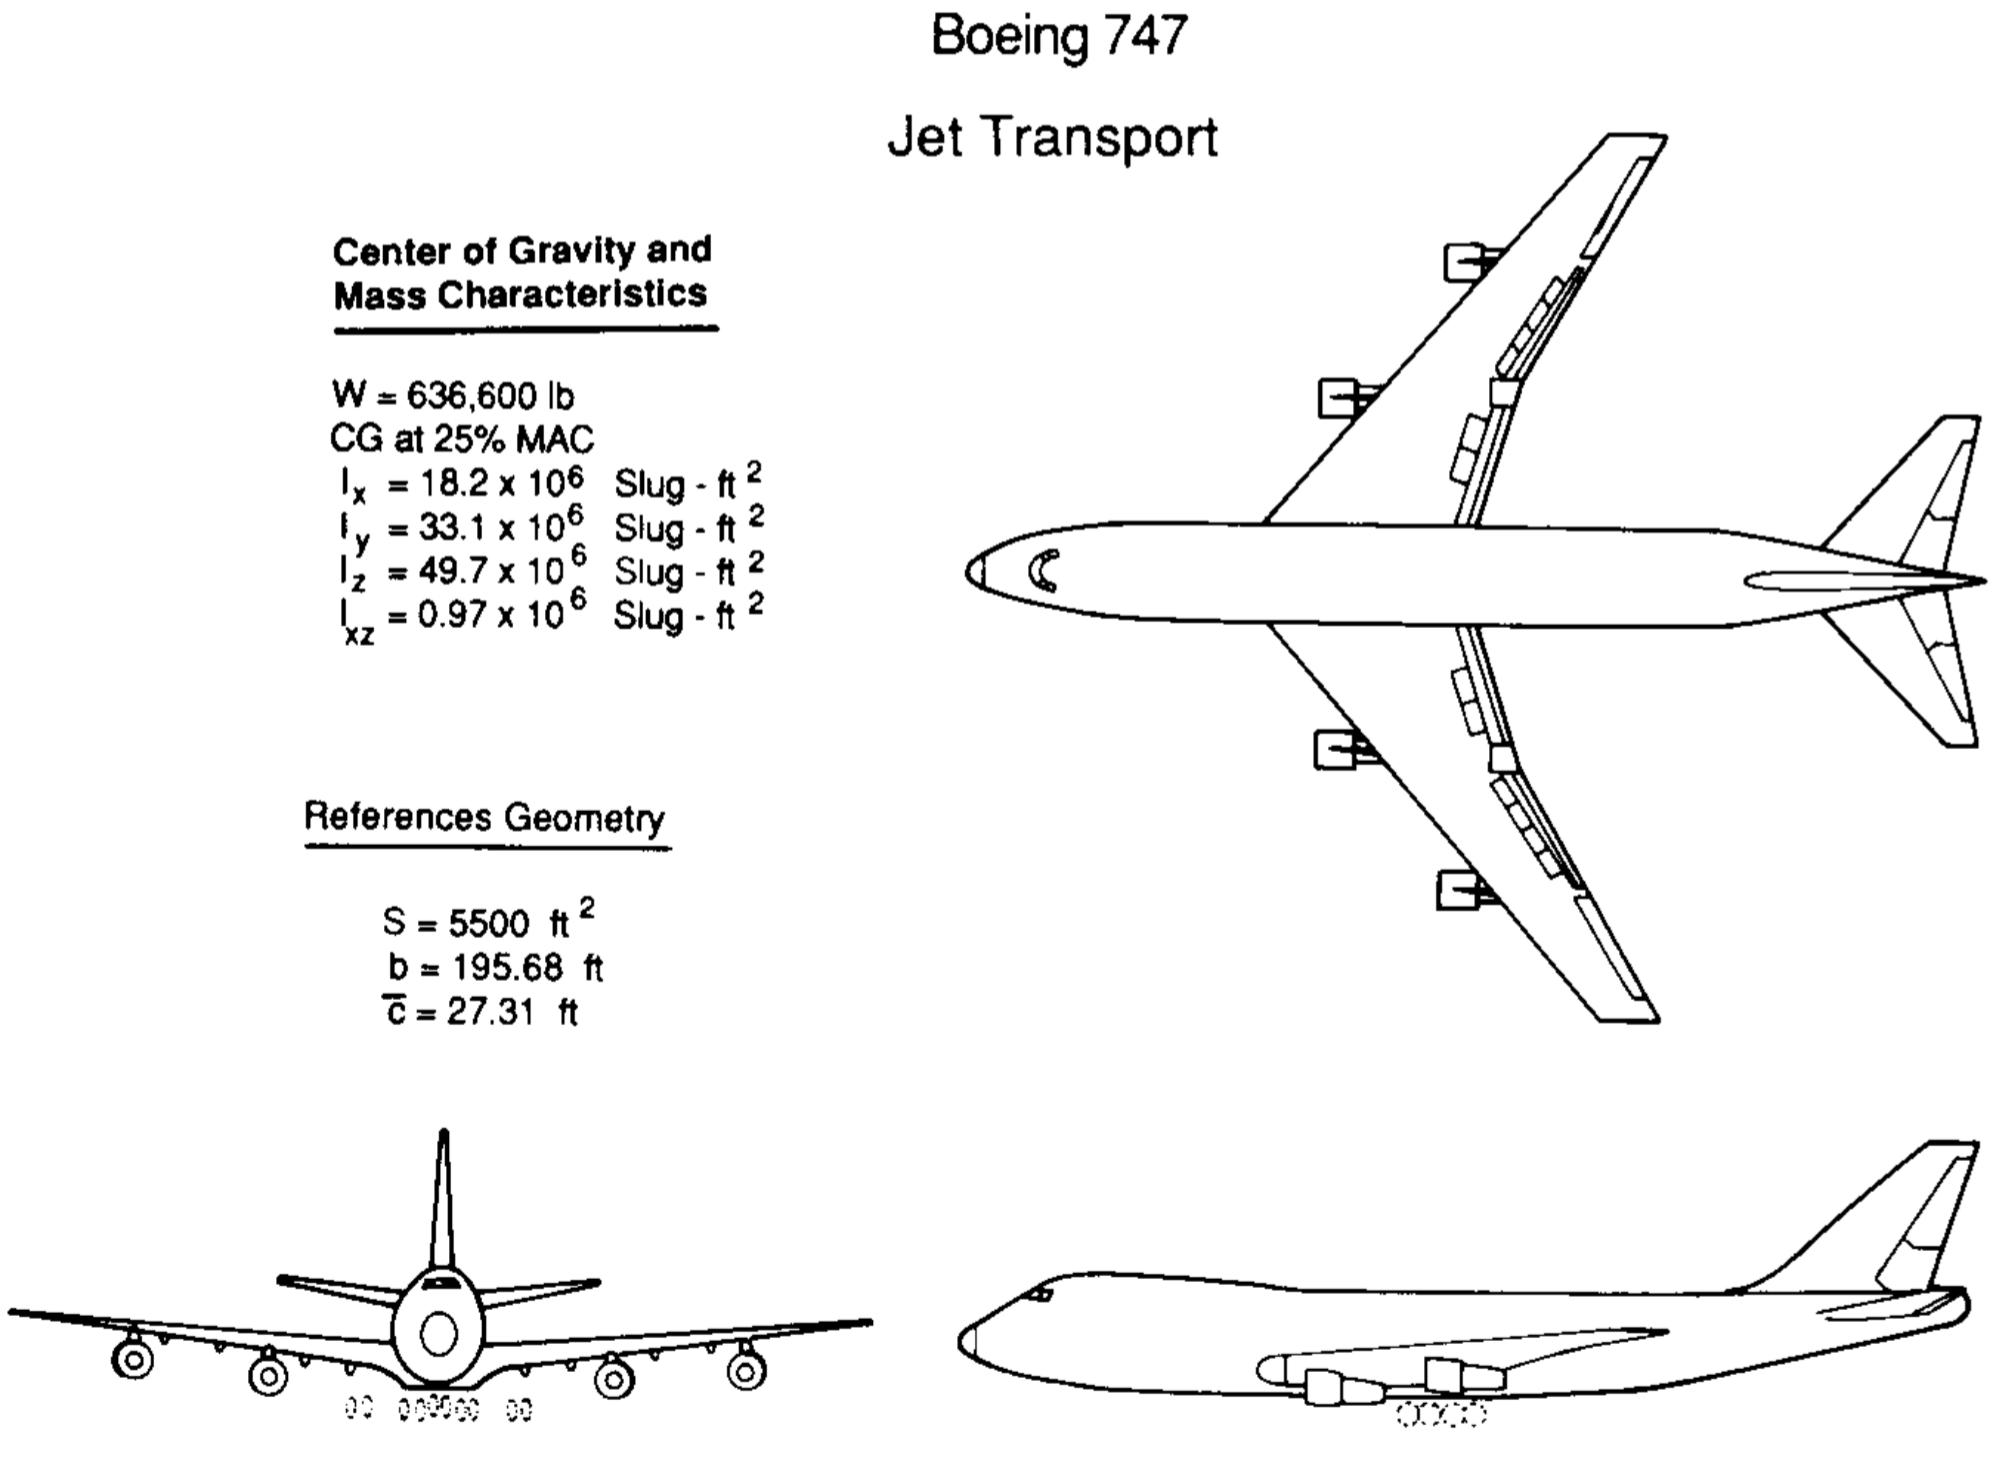
\includegraphics[width=4.5in]{\figurepath/transportLong.png}
    \vspace{-0.1in}
    \caption{Boeing 747--100 transport aircraft from Ref.\ \cite{nelson.flightcontrol.1998}.\label{fig.transportLong}}
  \end{center}
\end{figure}
The equations of motion describing the longitudinal dynamics of a transport aircraft such as the 747--100 during steady, level flight are given by the following
\begin{equation}
  \label{eqn.transportAircraftWhole}
  \begin{bmatrix}
    \dot{\alpha} \\
    \dot{q} \\
    \dot{\theta} \\
    \dot{h}
  \end{bmatrix}=
  \begin{bmatrix}
    \frac{Z_{\alpha}}{v_{\text{eq}}} & 1 & 0 & 0 \\
    M_{\alpha}+\frac{M_{\dot{\alpha}}Z_{\alpha}}{v_{\text{eq}}} & M_{q}+M_{\dot{\alpha}} & 0 & 0 \\
    0 & 1 & 0 & 0 \\
    -v_{\text{eq}} & 0 & v_{\text{eq}} & 0 \\
  \end{bmatrix}
  \begin{bmatrix}
    \alpha \\
    q \\
    \theta \\
    h
  \end{bmatrix}+
  \begin{bmatrix}
    \frac{Z_{\delta_{e}}}{v_{\text{eq}}} \\
    M_{\delta_{e}} \\
    0 \\
    0
  \end{bmatrix}
  \delta_{e}
\end{equation}
where $\alpha$ is the angle-of-attack, $q$ is the pitch rate, $\theta$ the pitch angle, $h$ is the altitude, and $\delta_{e}$ is the elevator deflection angle.
Considering uncertainty in the aerodynamic moment coefficients $M_{\alpha}$ and $M_{q}$, this system is represented by Eq.\ \eqref{eqn.wholeSystemUncertain}.
Partitioning\ \eqref{eqn.transportAircraftWhole} as described in Chapter~\ref{ch.Introduction}, the inner-loop dynamics in the form of\ \eqref{eqn.innerLoopDynamicsUncertain} and outer-loop dynamics as in\ \eqref{eqn.outerLoopDynamics} are obtained.
The following numerical values were selected from Ref.\ \cite{heffley.nasacr2144.1972, nelson.flightcontrol.1998}
\begin{equation*}
  \begin{aligned}
    v_{\text{eq}} &= 871 \text{~ft/s} \\
    Z_{\alpha} &= -349 \text{~ft/s}^{2} \\
    M_{\alpha} &= -1.65 \text{~rad/s}^{2} \\
    M_{\dot{\alpha}} &= -0.139 \text{~rad/s} \\
    M_{q} &= -0.401 \text{~rad/s} \\
    M_{\delta_{e}} &= -1.22 \text{~rad/s}^{2} \\
    Z_{\delta_{e}} &= -18.6 \text{~ft/s}^{2}
  \end{aligned}
\end{equation*}
The inner-loop control goal is to stabilize the system using only pitch rate measurement, with this output serving as both the measured and regulated outputs, leading to the following inner-loop dynamics
\begin{equation}
  \label{eqn.transportAircraftInnerLoop}
  \begin{split}
    \begin{bmatrix}
      \dot{\alpha} \\
      \dot{q}
    \end{bmatrix}
    &=
    \begin{bmatrix}
      \frac{Z_{\alpha}}{v_{\text{eq}}} & 1 \\
      M_{\alpha}+\frac{M_{\dot{\alpha}}Z_{\alpha}}{v_{\text{eq}}} & M_{q}+M_{\dot{\alpha}} \\
    \end{bmatrix}
    \begin{bmatrix}
    \alpha \\
    q
    \end{bmatrix}+
    \begin{bmatrix}
      \frac{Z_{\delta_{e}}}{v_{\text{eq}}} \\
      M_{\delta_{e}}
    \end{bmatrix}
    \delta_{e} \\
    q &=
    \begin{bmatrix}
      0 & 1
    \end{bmatrix}
    \begin{bmatrix}
    \alpha \\
    q
    \end{bmatrix}
  \end{split}
\end{equation}
The following uncertainty was selected, which is equivalent to uncertainty in the moment coefficients.
In addition, there is a reduction in the control effectiveness of the elevator to 50\% its nominal value.
\begin{equation*}
  \begin{split}
    \Psi_{p}
    &=
    \begin{bmatrix}
      4 & -4
    \end{bmatrix}^{\top} \\
    \Lambda
    &=
    0.5
  \end{split}
\end{equation*}
The following weighting matrices were used to design the LQR inner-loop baseline controller
\begin{equation*}
  \begin{split}
    Q_{\text{lqr}}
    &=
    \text{diag}\bigr(
    \begin{bmatrix}
      0 & 0 & 1000
    \end{bmatrix}\bigr) \\
    R_{\text{lqr}}
    &=
    1
  \end{split}
\end{equation*}
The following upper-bound on the uncertainty was used
\begin{equation*}
  \Psi_{\text{max}} = 1000
\end{equation*}
resulting in $X$ in\ \eqref{eqn.Px} given by
\begin{equation*}
  X =
  \begin{bmatrix}
    1.0005 & 1 \\
    1 & 2199
  \end{bmatrix}
\end{equation*}
This inner-loop adaptive controller was then implemented in a simulation of the aircraft model, resulting in the response shown in Fig.~\ref{fig.innerLoopTransportLong}.
Unlike the pendulum model, the kinematics of the aircraft, the pitch angle and altitude, do not couple into the inner-loop short-period dynamics at all.
Thus, the assumption that $B_{gd}=0$ in Eq.\ \eqref{eqn.wholeSystemUncertain} is satisfied exactly.
At $t=10$ seconds uncertainty is introduced, but the adaptive controller is not activated until $t=30$ seconds.

\newpage
\begin{figure}[H]
  \hspace{-0.0in}
  \noindent\makebox[6.5in]{%
  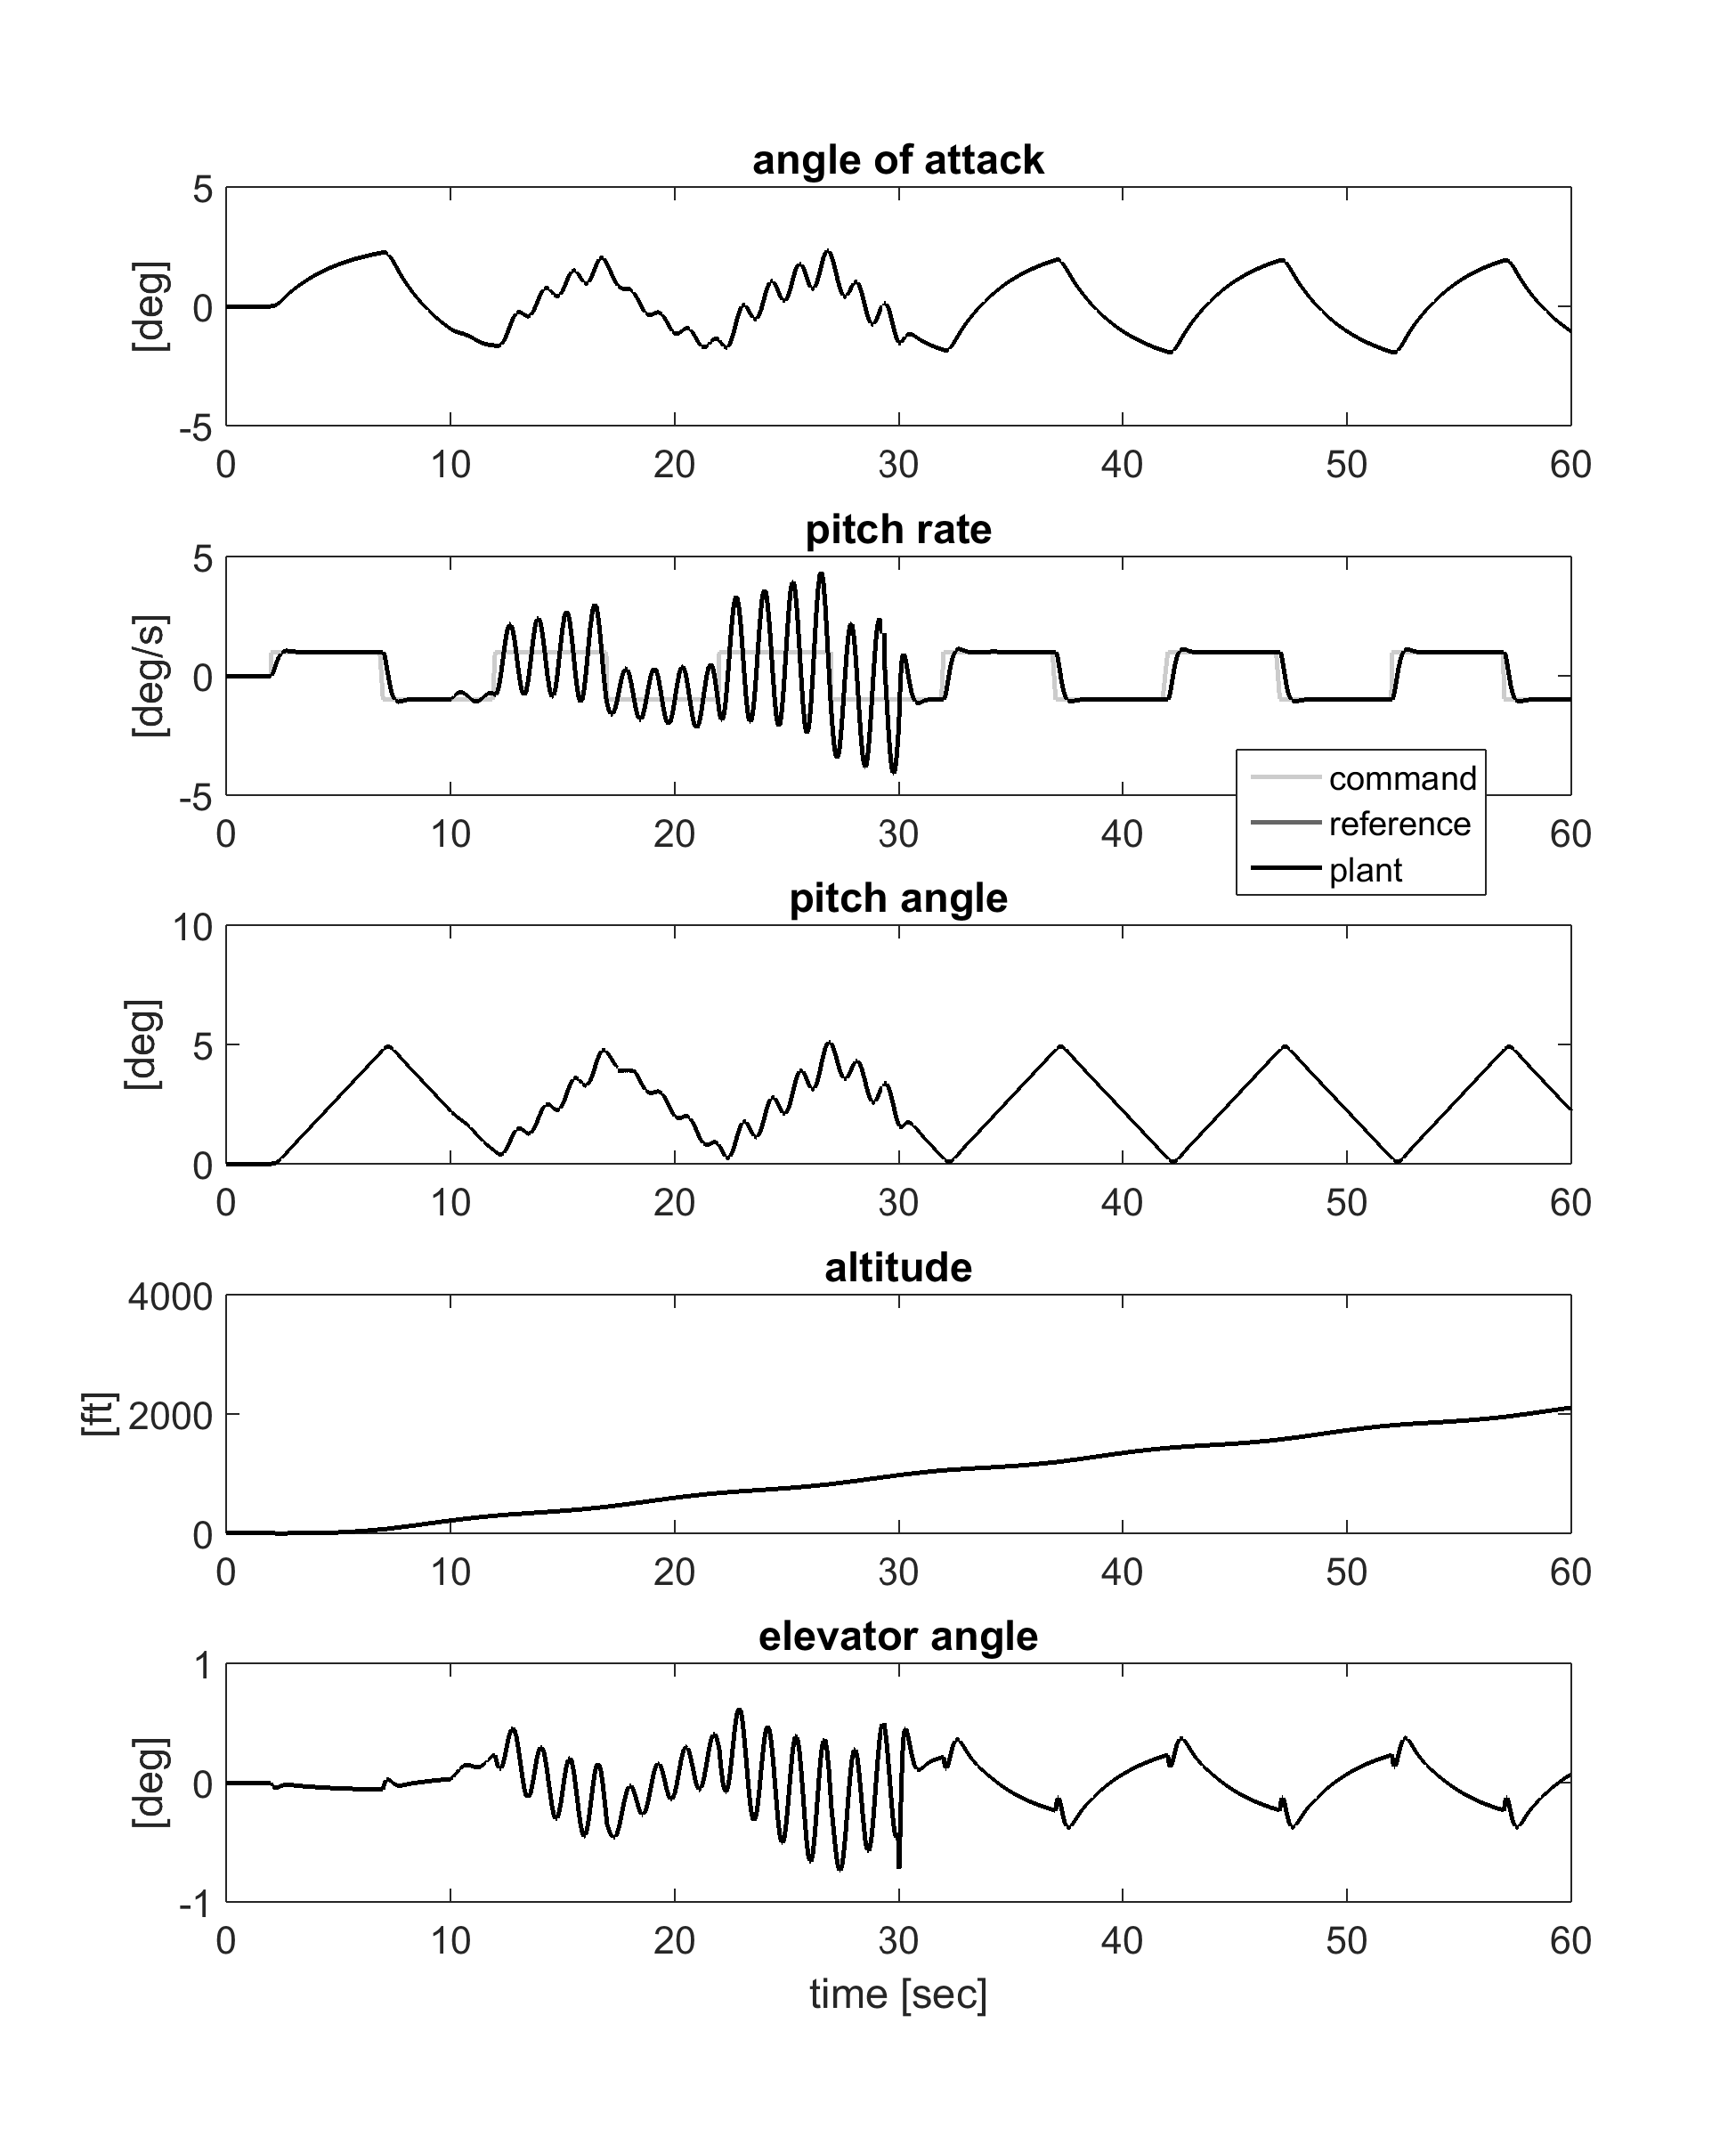
\includegraphics[width=6.5in]{\figurepath/innerLoopTransportLong.png}}
  \vspace{-0.95in}
  \caption{Time response of transport aircraft with inner-loop controller.\label{fig.innerLoopTransportLong}}
\end{figure}

\section{Conclusion}\label{sec.innerLoopConclusion}

This chapter presented a new alternative method for synthesizing a CRM based output feedback adaptive controller for a class of uncertain MIMO systems which do not have any unstable transmission zeros.
The controller is composed of a baseline control gain augmented with an adaptive component to accommodate control effectiveness uncertainty and matched plant uncertainty, and makes use of the closed-loop reference model to improve the transient properties of the overall adaptive system.
The adaptive controller requires the underlying error dynamics be made SPR through the synthesis of the postcompensator $S_{1}$ and CRM gain $L$.
The SPR relationship is enforced by reducing an underlying bilinear matrix inequality to a feasible linear matrix inequality through appropriate selection of a tuning matrix $X$.
The procedure does not require the plant first be squared-up.
It is computationally simple, and it requires only the calculation of some generalized inverses, the solution of the Lyapunov equation, and the solution of a reduced order state feedback problem.
This procedure is summarized in nine straightforward steps.
Furthermore, the degrees of freedom in the tuning matrix $X$ capture a large subset of all possible solutions which ensure the SPR property.
Using these degrees of freedom, $X$ can be tuned to provide the desired stability margins for the baseline system, as well as a globally stable update law.
The result is a baseline output feedback controller with good stability margins and adaptive augmentation capable of accommodating matched uncertainties.

This inner-loop design provided a controller capable of enforcing bounded reference tracking of $z_{p,\text{cmd}}(t)$ by $z_{p}(t)$, and accommodating uncertainties.
With the design of this inner-loop adaptive controller complete, the original control goal described in Chapter~\ref{ch.Introduction} has not yet been satisfied.
Recall that this control goal ultimately requires $u(t)$ in\ \eqref{eqn.wholeSystemUncertain} to be designed such that $z_{g}(t)$ tracks $z_{g,\text{cmd}}(t)$.
With the inner-loop designed providing $u(t)$ such that $z_{p}(t)$ tracks $z_{p,\text{cmd}}(t)$, the problem now becomes how to prescribe $z_{p,\text{cmd}}(t)$ such that $z_{g}(t)$ tracks $z_{g,\text{cmd}}(t)$.
The solution to this problem is described in Chapter~\ref{ch.outerLoop} which utilizes the existing inner-loop control design, but reintroduces the $B_{gd}$ term as in\ \eqref{eqn.innerLoopDynamicsUncertain} and considers the outer-loop dynamics in\ \eqref{eqn.outerLoopDynamics}.

\chapter{Outer-Loop Control Design}\label{ch.outerLoop}

This chapter presents an outer-loop control design for uncertain systems represented in\ \eqref{eqn.wholeSystemUncertain} which already have an adaptive inner-loop controller designed as described in Chapter~\ref{ch.innerLoop}.
The outer-loop controller presented in this chapter is designed around the system with closed adaptive inner loop, uses fixed-gains, and guarantees stability of the closed-loop system.
The outer-loop uses components of a closed-loop reference model, and generates the appropriate commands for the inner loop $z_{p,\text{cmd}}(t)$ such that the outer-loop regulated output $z_{g}(t)$ tracks the desired outer-loop command $z_{g,\text{cmd}}^{\prime}(t)$ with bounded errors.
The design of the outer-loop utilizes the existing inner-loop design, which has been designed to have good stability margins and the desired time-response characteristics.
While certain features are added to the inner-loop controller, this outer-loop design does not require any changes to any of the existing inner-loop control gains.
In addition, an state limiter is proposed in Section~\ref{sec.outerLoop.stateLimiting} which is incorporated into the outer-loop control design and limits the inner-loop command generated by the outer-loop controller.
This limiting is done so as to prevent state variables from exceeding certain limits, or to simply restrict the inner-loop command from becoming too large.
The proposed outer-loop controller is designed to be added around the existing inner-loop, and generate the inner-loop commands, as shown in Figure~\ref{fig.innerLoopWithStartOfOuterLoop} below.
In this figure, the unlabeled inputs to the inner and outer-loop controllers represent additional feedback signals that will be used to ensure stability and enforce command tracking, which have yet to be determined.
This architecture was first presented in Ref.\ \cite{wiese.sequential.2016} for the case of state feedback, that is systems in the form of Eq.\eqref{eqn.wholeSystemUncertain} where $C_{p}=I$ and $C_{g}=I$.

\begin{figure}[H]
  \begin{center}
    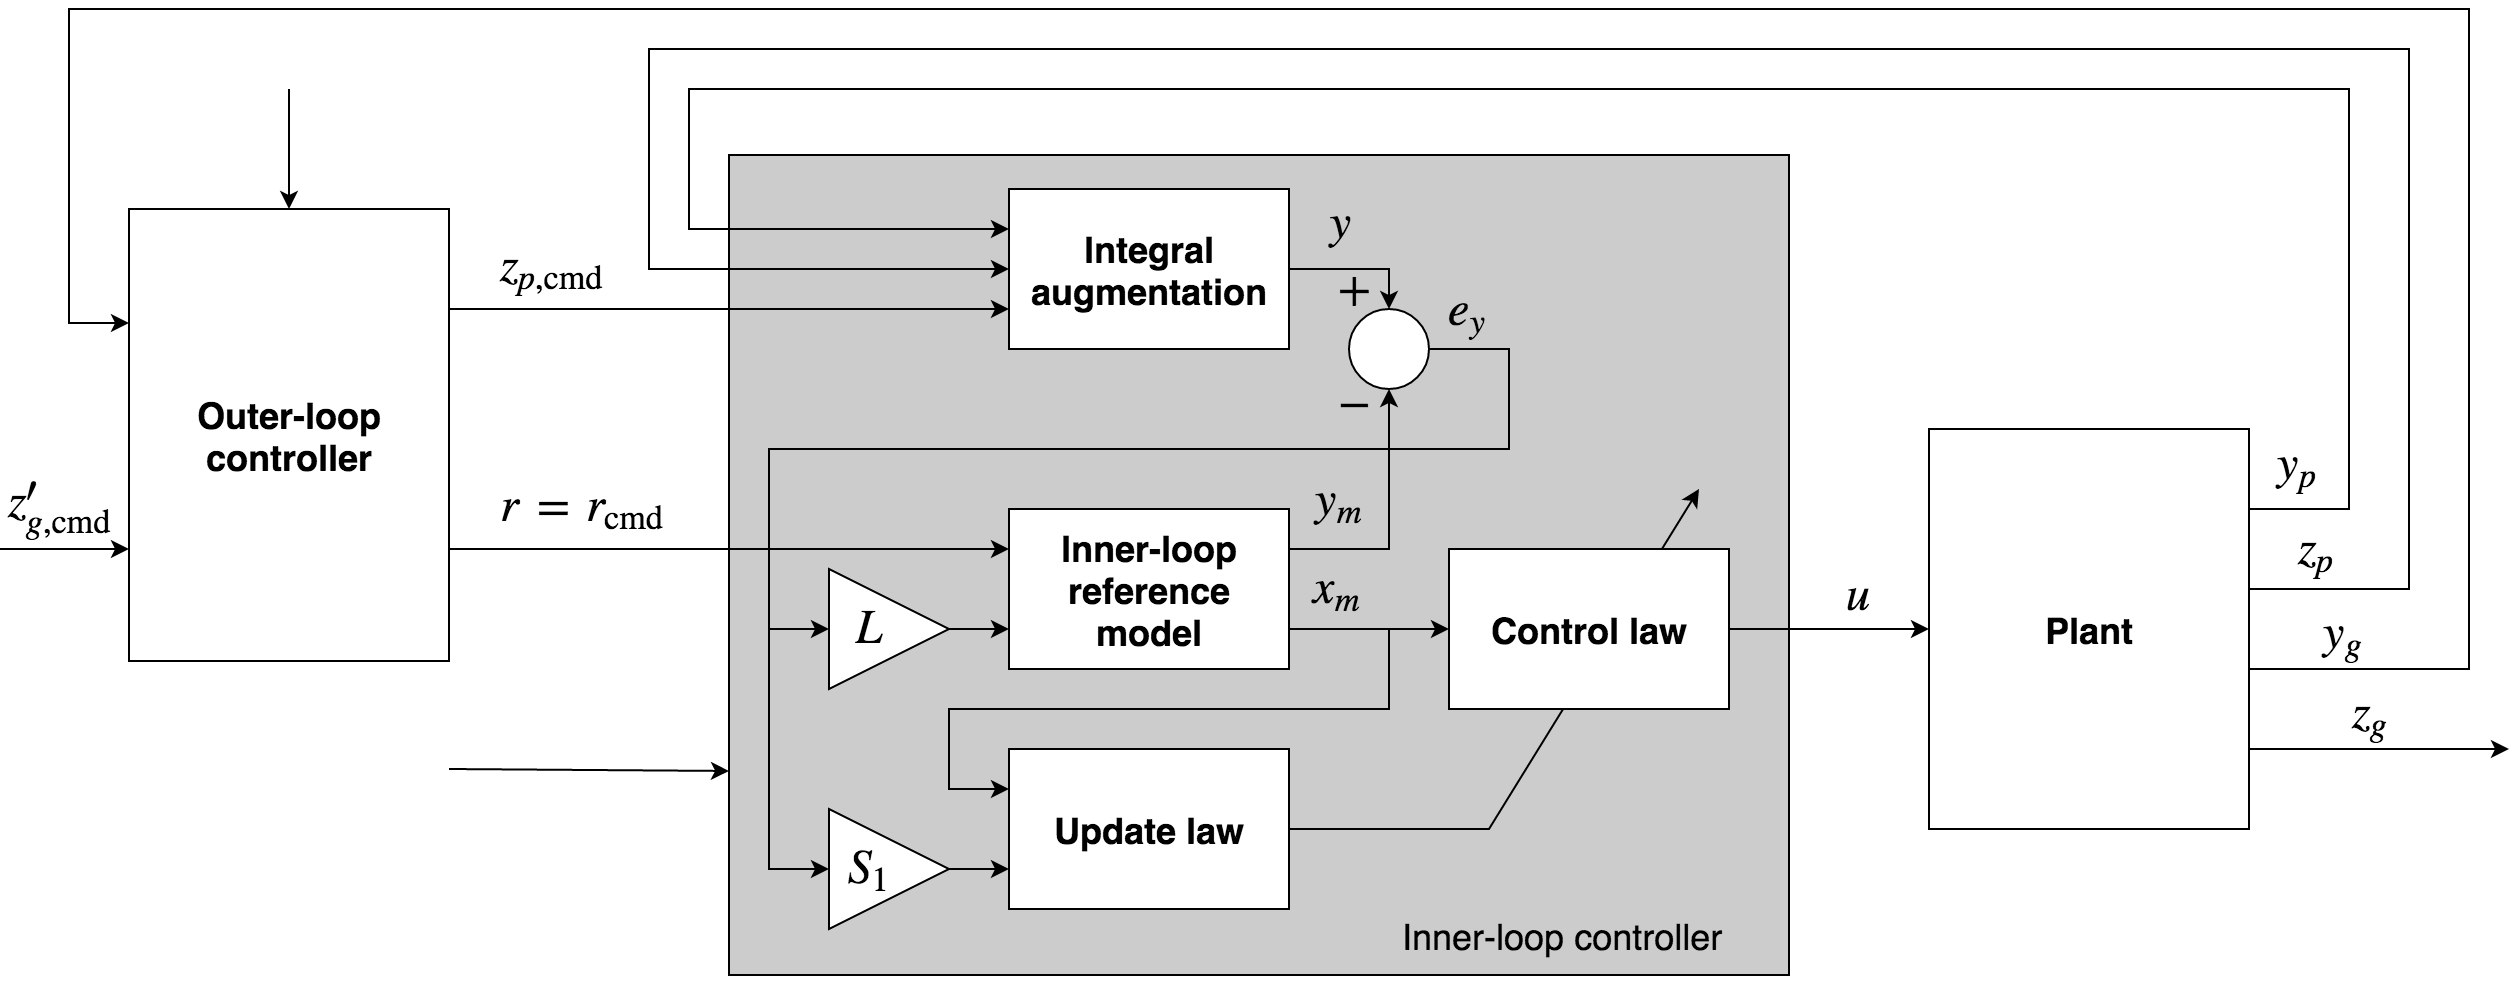
\includegraphics[width=6.5in]{\figurepath/innerLoopWithStartOfOuterLoop.png}
    \vspace{-0.1in}
    \caption{Outer-loop control architecture block diagram.\label{fig.innerLoopWithStartOfOuterLoop}}
  \end{center}
\end{figure}

\section{Outer-Loop Control Architecture}

In this section the outer-loop control architecture is proposed, which consists of two additional reference model components, and some additional outer-loop static feedback gains, two of which are CRM gains.
This architecture is presented, and conditions on the selection of the feedback gains to guarantee global stability of the closed-loop system is given.

In designing the outer-loop controller, the Assumption that $B_{gd}$ in\ \eqref{eqn.innerLoopDynamicsUncertain} is zero is relaxed.
By including the $B_{gd}$ term in\ \eqref{eqn.innerLoopDynamicsUncertain} and using the same integral augmentation, the system in\ \eqref{eqn.uncsystem} becomes
\begin{equation}
  \label{eqn.uncsystemWithBd}
  \begin{split}
    \dot{x}(t) &= Ax(t) + B\bigr(\Lambda u(t)+\Psi^{\top}x(t)\bigr)+B_{\text{cmd}}z_{p,\text{cmd}}(t) + B_{d}x_{g}(t) \\
    y(t) &= Cx(t) \\
  \end{split}
\end{equation}
where $B_{d}\in\mathbb{R}^{n\times n_{g}}$ is given by
\begin{equation*}
  B_{d} =
  \begin{bmatrix}
    B_{gd} \\
    0_{n_{ep}\times n_{g}} \\
  \end{bmatrix}
\end{equation*}
To accommodate the $B_{d}$ term in\ \eqref{eqn.uncsystemWithBd}, the inner-loop reference model in\ \eqref{eqn.refmodel} is modified as
\begin{equation}
  \label{eqn.refmodelWithBd}
  \begin{split}
    \dot{x}_{m}(t) &= A_{m}x_{m}(t) + B_{\text{cmd}}r(t) + L\bigr(y_{m}(t)-y(t)\bigr) + B_{d}x_{gm}(t) \\
    y_{m}(t) &= Cx_{m}(t)
  \end{split}
\end{equation}
This change with the addition of the $B_{d}$ term in the plant in\ \eqref{eqn.uncsystemWithBd} and reference model in\ \eqref{eqn.refmodelWithBd} modifies the inner-loop error dynamics in\ \eqref{eqn.errordynamics1} as follows
\begin{equation}
  \label{eqn.errordynamics4}
  \begin{split}
    \dot{e}_{x}(t) &= (A+LC+B\Psi^{\top})e_{x}(t)+B\Lambda\widetilde{\Theta}^{\top}(t)x_{m}(t) + B_{\text{cmd}}\bigr(z_{p,\text{cmd}}(t) - r(t)\bigr) + B_{d}e_{g}(t) \\
    e_{y}(t) &= Ce_{x}(t) \\
  \end{split}
\end{equation}
The next step is to consider the outer-loop dynamics in\ \eqref{eqn.outerLoopDynamics} and generate the reference signals $r(t)$ and $z_{p,\text{cmd}}(t)$ in\ \eqref{eqn.errordynamics4} so that $z_{g}(t)$ tracks $z_{g,\text{cmd}}(t)$ with bounded errors.
Asymptotic tracking of an arbitrary bounded command $z_{g,\text{cmd}}(t)$ by $z_{g}(t)$ is not possible.
However, in the same way that the inner-loop reference model essentially serves as a command pre-filter for $z_{p,\text{cmd}}(t)$ generating $z_{pm}(t)$ for which asymptotic tracking by $z_{p}(t)$ is possible, a similar filtered version of $z_{g,\text{cmd}}(t)$ for which asymptotic tracking is possible, is created.
For this, some additional outer-loop reference model components are required.

\subsection{Reference Model Design}

\subsubsection{Outer-Loop Reference Model}

An additional outer-loop reference model is introduced in addition to the inner-loop reference model in\ \eqref{eqn.refmodelWithBd} as
\begin{equation}
  \label{eqn.refmodelouter}
  \begin{split}
    \dot{x}_{gm}(t) &= A_{g}x_{gm}(t) + B_{g}x_{m}(t) + L_{y}\bigr(y_{m}(t)-y(t)\bigr) + L_{g}\bigr(y_{gm}(t)-y_{g}(t)\bigr) \\
    y_{gm}(t) &= C_{g}x_{gm}(t) \\
    z_{gm}(t) &= C_{gz}x_{gm}(t) \\
  \end{split}
\end{equation}
where $L_{y}\in\mathbb{R}^{n_{g}\times p}$, and $L_{g}\in\mathbb{R}^{n_{g}\times p_{g}}$.
The outer-loop tracking error is given by
\begin{equation*}
  e_{g}(t) = x_{g}(t) - x_{gm}(t)
\end{equation*}
and the measured outer-loop error by
\begin{equation*}
  e_{gy}(t) = y_{g}(t) - y_{gm}(t)
\end{equation*}
and the goal is to design an outer-loop controller such that $\lim_{t\rightarrow\infty}e_{g}(t)=0$, which will thus enforce the outer-loop tracking as desired.

\begin{rem-dan}\label{rem.ygmandzgm}
  With the structure of the measured and regulated outputs in the outer-loop reference model component\ \eqref{eqn.refmodelouter} where unlike the inner-loop reference model\ \eqref{eqn.refmodel} the regulated output has no direct feedthrough, the measured output matrix is selected so as to contain the regulated output as well.
  That is, the matrix $C_{g}$ in\ \eqref{eqn.refmodelouter} is expressed as
  \begin{equation*}
    C_{g} =
    \begin{bmatrix}
      C_{gy} \\
      C_{gz}
    \end{bmatrix}
  \end{equation*}
\end{rem-dan}

Subtracting the outer-loop dynamics\ \eqref{eqn.outerLoopDynamics} and the outer-loop reference model\ \eqref{eqn.refmodelouter} gives the following outer-loop error dynamics
\begin{equation*}
  \begin{split}
    \dot{e}_{g}(t) &=
    A_{g}x_{g}(t)
    + B_{g}x(t)
    - A_{g}x_{gm}(t)
    - B_{g}x_{m}(t)
    - L_{y}\bigr(y_{m}(t)-y(t)\bigr)
    - L_{g}\bigr(y_{gm}(t)-y_{g}(t)\bigr) \\
    &=
    A_{g}\bigr(x_{g}(t) - x_{gm}(t)\bigr)
    + B_{g}\bigr(x(t) - x_{m}(t)\bigr)
    + L_{y}C\bigr(x(t)-x_{m}(t)\bigr)
    + L_{g}C_{g}\bigr(x_{g}(t)-x_{gm}(t)\bigr) \\
    &=
    A_{g}e_{g}(t)
    + B_{g}e_{x}(t)
    + L_{y}Ce_{x}(t)
    + L_{g}C_{g}e_{g}(t)
  \end{split}
\end{equation*}
giving
\begin{equation}
  \label{eqn.outerlooperrordynamics}
  \begin{split}
    \dot{e}_{g}(t) &= \bigr(A_{g} + L_{g}C_{g}\bigr)e_{g}(t) + \bigr(B_{g} + L_{y}C\bigr)e_{x}(t) \\
    e_{gy}(t) &= C_{g}e_{g}(t) \\
  \end{split}
\end{equation}

\subsubsection{Forward-loop Reference Model}

Combining the inner-loop reference model in\ \eqref{eqn.refmodelWithBd} and the outer-loop reference model in\ \eqref{eqn.refmodelouter}, the combined reference model is obtained as
\begin{equation}
  \label{eqn.refmodelcombined}
  \begin{split}
    \begin{bmatrix}
      \dot{x}_{m}(t) \\
      \dot{x}_{gm}(t) \\
    \end{bmatrix}
    &=
    \begin{bmatrix}
      A_{m} & B_{d} \\
      B_{g} & A_{g} \\
    \end{bmatrix}
    \begin{bmatrix}
      x_{m}(t) \\
      x_{gm}(t) \\
    \end{bmatrix}
    +
    \begin{bmatrix}
      B_{\text{cmd}} \\
      0
    \end{bmatrix} r(t)
    +
    \begin{bmatrix}
      L \\
      L_{y}
    \end{bmatrix}\bigr(y_{m}(t)-y(t)\bigr)
    +
    \begin{bmatrix}
      0 \\
      L_{g}
    \end{bmatrix}\bigr(y_{gm}(t)-y_{g}(t)\bigr) \\
    z_{gm}(t) &=
    \begin{bmatrix}
      0 & C_{gz}
    \end{bmatrix}
    \begin{bmatrix}
      x_{m}(t) \\
      x_{gm}(t) \\
    \end{bmatrix}
  \end{split}
\end{equation}
The forward-loop controller which generates the reference model input command $r(t)$ from the outer-loop command signal $z_{g,\text{cmd}}^{\prime}(t)$ is now designed.
Furthermore, this forward-loop reference model must ensure the complete resulting reference model, given by Eq.\ \eqref{eqn.refmodelcombined} with the forward-loop reference model, is stable.
A control of the follow form is selected
\begin{equation}
  \label{eqn.forwardloopcontroller}
  \begin{split}
    \dot{x}_{fm}(t) &= A_{fm}x_{fm}(t) + B_{f1}z_{g,\text{cmd}}(t) + B_{f2}x_{gm}(t) + B_{f3}x_{m}(t) \\
    r_{\text{cmd}}(t) &= C_{fm}x_{fm}(t) + D_{f1}z_{g,\text{cmd}}(t) + D_{f2}x_{gm}(t) + D_{f3} x_{m}(t) \\
  \end{split}
\end{equation}
where the matrices $A_{fm}\in\mathbb{R}^{n_{f}\times n_{f}}$, $B_{f1}\in\mathbb{R}^{n_{f}\times n_{eg}}$, $B_{f2}\in\mathbb{R}^{n_{f}\times n_{g}}$, $B_{f3}\in\mathbb{R}^{n_{f}\times n}$, $C_{fm}\in\mathbb{R}^{n_{ep}\times n_{f}}$, $D_{f1}\in\mathbb{R}^{n_{ep}\times n_{eg}}$, $D_{f2}\in\mathbb{R}^{n_{ep}\times n_{g}}$, and $D_{f3}\in\mathbb{R}^{n_{ep}\times n}$ are selected so the closed loop system given by combining\ \eqref{eqn.forwardloopcontroller} and\ \eqref{eqn.refmodelcombined} provides steady-state command tracking of $z_{g,\text{cmd}}(t)$ by $z_{gm}(t)$ when the errors $e_{y}(t)$ and $e_{gy}(t)$ are zero.
Furthermore, we set the outer-loop command $z_{g,\text{cmd}}(t)$ in\ \eqref{eqn.forwardloopcontroller} equal to the desired outer-loop command $z_{g,\text{cmd}}^{\prime}(t)$ as
\begin{equation}
  \label{eqn.zgcmdzgcmdprime}
  z_{g,\text{cmd}}(t) = z_{g,\text{cmd}}^{\prime}(t)
\end{equation}
Set $r(t)$ in\ \eqref{eqn.refmodelcombined} using the output from the forward-loop reference model component in\ \eqref{eqn.forwardloopcontroller} as
\begin{equation}
  \label{eqn.rrcmd}
  r(t) = r_{\text{cmd}}(t)
\end{equation}
Substituting the forward-loop controller\ \eqref{eqn.forwardloopcontroller} into\ \eqref{eqn.refmodelcombined} gives the following
\begin{equation}
  \label{eqn.fullOpenLoopReferenceModel}
  \begin{split}
    \begin{bmatrix}
      \dot{x}_{m}(t) \\
      \dot{x}_{gm}(t) \\
      \dot{x}_{fm}(t) \\
    \end{bmatrix}
    &=
    \begin{bmatrix}
      A_{m} & B_{d} & 0 \\
      B_{g} & A_{g} & 0 \\
      B_{f3} & B_{f2} & A_{fm} \\
    \end{bmatrix}
    \begin{bmatrix}
      x_{m}(t) \\
      x_{gm}(t) \\
      x_{fm}(t) \\
    \end{bmatrix}
    +
    \begin{bmatrix}
      B_{\text{cmd}} \\
      0 \\
      0 \\
    \end{bmatrix} r(t)
    +
    \begin{bmatrix}
      L \\
      L_{y} \\
      0 \\
    \end{bmatrix}\bigr(y_{m}(t)-y(t)\bigr) \\
    & \qquad +
    \begin{bmatrix}
      0 \\
      L_{g} \\
      0 \\
    \end{bmatrix}\bigr(y_{gm}(t)-y_{g}(t)\bigr)
    +
    \begin{bmatrix}
      0 \\
      0 \\
      B_{f1} \\
    \end{bmatrix}z_{g,\text{cmd}}(t) \\
    r_{\text{cmd}}(t)
    &=
    \begin{bmatrix}
      D_{f3} & D_{f2} & C_{fm}
    \end{bmatrix}
    \begin{bmatrix}
      x_{m}(t) \\
      x_{gm}(t) \\
      x_{fm}(t) \\
    \end{bmatrix}
    + D_{f1}z_{g,\text{cmd}}(t) \\
  \end{split}
\end{equation}
The entire complete reference model\ \eqref{eqn.fullOpenLoopReferenceModel} can be written more compactly as
\begin{equation}
  \label{eqn.xbareqnopenloop}
  \begin{split}
    \dot{\bar{x}}_{m}(t) &= \bar{A}\bar{x}_{m}(t) + \bar{B}r(t) - \bar{L}_{y}e_{y}(t) - \bar{L}_{g}e_{gy}(t) + \bar{B}_{m}z_{g,\text{cmd}}(t) \\
    r_{\text{cmd}}(t) &= \bar{C}_{m}\bar{x}_{m}(t) + D_{f1}z_{g,\text{cmd}}(t) \\
  \end{split}
\end{equation}
where the entire reference model state $\bar{x}_{m}(t)\in\mathbb{R}^{n+n_{g}+n_{f}}$ is given by
\begin{equation*}
  \bar{x}_{m}(t) =
  \begin{bmatrix}
    x_{m}^{\top}(t) & x_{gm}^{\top}(t) & x_{fm}^{\top}(t)
  \end{bmatrix}^{\top}
\end{equation*}
and where $\bar{A}\in\mathbb{R}^{n+n_{g}+n_{f}\times n+n_{g}+n_{f}}$, $\bar{B}\in\mathbb{R}^{n+n_{g}+n_{f}\times n_{ep}}$, $\bar{L}_{y}\in\mathbb{R}^{n+n_{g}+n_{f}\times p}$, $\bar{L}_{g}\in\mathbb{R}^{n+n_{g}+n_{f}\times p_{g}}$, $\bar{B}_{m}\in\mathbb{R}^{n+n_{g}+n_{f}\times n_{eg}}$, and $\bar{C}_{m}\in\mathbb{R}^{n_{ep} \times n+n_{g}+n_{f}}$ are given by
\begin{equation*}
  \begin{gathered}
    \bar{A} =
    \begin{bmatrix}
      A_{m} & B_{d} & 0 \\
      B_{g} & A_{g} & 0 \\
      B_{f3} & B_{f2} & A_{fm} \\
    \end{bmatrix}
    \quad
    \bar{B} =
    \begin{bmatrix}
      B_{\text{cmd}} \\
      0 \\
      0 \\
    \end{bmatrix}
    \quad
    \bar{L}_{y} =
    \begin{bmatrix}
      L \\
      L_{y} \\
      0 \\
    \end{bmatrix}
    \quad
    \bar{L}_{g} =
    \begin{bmatrix}
      0 \\
      L_{g} \\
      0 \\
    \end{bmatrix}
    \quad
    \bar{B}_{m} =
    \begin{bmatrix}
      0 \\
      0 \\
      B_{f1} \\
    \end{bmatrix} \\
    \bar{C}_{m} =
    \begin{bmatrix}
      D_{f3} & D_{f2} & C_{fm}
    \end{bmatrix}
  \end{gathered}
\end{equation*}
Setting the inner-loop reference model command $r(t)$ as in\ \eqref{eqn.rrcmd} and simplifying\ \eqref{eqn.fullOpenLoopReferenceModel} gives
\begin{equation}
  \label{eqn.refmodelcombinedwithforwardloop}
  \begin{split}
    \begin{bmatrix}
      \dot{x}_{m}(t) \\
      \dot{x}_{gm}(t) \\
      \dot{x}_{fm}(t) \\
    \end{bmatrix}
    &=
    \begin{bmatrix}
      A_{m}+B_{\text{cmd}}D_{f3} & B_{d} + B_{\text{cmd}}D_{f2} & B_{\text{cmd}}C_{fm} \\
      B_{g} & A_{g} & 0 \\
      B_{f3} & B_{f2} & A_{fm} \\
    \end{bmatrix}
    \begin{bmatrix}
      x_{m}(t) \\
      x_{gm}(t) \\
      x_{fm}(t)
    \end{bmatrix}
    +
    \begin{bmatrix}
      B_{\text{cmd}}D_{f1} \\
      0 \\
      B_{f1} \\
    \end{bmatrix} z_{g,\text{cmd}}(t) \\
    &\quad+
    \begin{bmatrix}
      L \\
      L_{y} \\
      0 \\
    \end{bmatrix}\bigr(y_{m}(t)-y(t)\bigr)
    +
    \begin{bmatrix}
      0 \\
      L_{g} \\
      0 \\
    \end{bmatrix}\bigr(y_{gm}(t)-y_{g}(t)\bigr) \\
    r(t)
    &=
    \begin{bmatrix}
      D_{f3} & D_{f2} & C_{fm}
    \end{bmatrix}
    \begin{bmatrix}
      x_{m}(t) \\
      x_{gm}(t) \\
      x_{fm}(t) \\
    \end{bmatrix}
    + D_{f1}z_{g,\text{cmd}}(t) \\
  \end{split}
\end{equation}
which can be represented more compactly as
\begin{equation}
  \label{eqn.compactreferencemodel}
  \begin{split}
    \dot{\bar{x}}_{m}(t) &= \bar{A}_{m}\bar{x}_{m}(t) + \bar{B}_{\text{cmd}}z_{g,\text{cmd}}(t) - \bar{L}_{y}e_{y}(t) - \bar{L}_{g}e_{gy}(t) \\
    r_{\text{cmd}}(t) &= \bar{C}_{m}\bar{x}_{m}(t) + D_{f1}z_{g,\text{cmd}}(t) \\
  \end{split}
\end{equation}
where $\bar{A}_{m}\in\mathbb{R}^{n+n_{g}+n_{f}\times n+n_{g}+n_{f}}$ and $\bar{B}_{\text{cmd}}\in\mathbb{R}^{n+n_{g}+n_{f}\times n_{eg}}$ are given by
\begin{equation}
  \bar{A}_{m} =
  \begin{bmatrix}
    A_{m}+B_{\text{cmd}}D_{f3} & B_{d} + B_{\text{cmd}}D_{f2} & B_{\text{cmd}}C_{fm} \\
    B_{g} & A_{g} & 0 \\
    B_{f3} & B_{f2} & A_{fm} \\
  \end{bmatrix}
  \qquad
  \bar{B}_{\text{cmd}} =
  \begin{bmatrix}
    B_{\text{cmd}}D_{f1} \\
    0 \\
    B_{f1} \\
  \end{bmatrix}
\end{equation}
where $\bar{A}_{m} = \bar{A}+\bar{B}\bar{C}_{m}$.
Appropriate selection of the controller in\ \eqref{eqn.forwardloopcontroller} ensures that $\bar{A}_{m}$ in\ \eqref{eqn.compactreferencemodel} is Hurwitz.
Combining the integral augmented, uncertain inner-loop dynamics in\ \eqref{eqn.uncsystemWithBd} with the outer-loop guidance dynamics\ \eqref{eqn.outerLoopDynamics} and reference model\ \eqref{eqn.compactreferencemodel} the following system is obtained
\begin{equation}
  \label{eqn.plantAndCompactReferenceModel}
  \begin{aligned}
    \dot{x}(t)
    &=
    Ax(t) + B\bigr(\Lambda u(t)+\Psi^{\top}x(t)\bigr) + B_{\text{cmd}}z_{p,\text{cmd}}(t) + B_{d}x_{g}(t) \\
    y(t)
    &=
    Cx(t) \\
    \dot{x}_{g}(t)
    &=
    A_{g}x_{g}(t) + B_{g}x(t) \\
    y_{g}(t)
    &=
    C_{g}x_{g}(t) \\
    \dot{\bar{x}}_{m}
    &=
    \bar{A}_{m}\bar{x}_{m}(t) + \bar{B}_{\text{cmd}}z_{g,\text{cmd}}(t) - \bar{L}_{y}e_{y}(t) - \bar{L}_{g}e_{gy}(t) \\
    r_{\text{cmd}}
    &=
    \bar{C}_{m}\bar{x}_{m}(t) + D_{f1}z_{g,\text{cmd}}(t)
  \end{aligned}
\end{equation}
where only the specification of $z_{p,\text{cmd}}(t)$ remains to completely specify the control architecture.

\begin{rem-dan}
  One possible selection for the forward-loop reference model in\ \eqref{eqn.forwardloopcontroller} is that of an LQR-PI controller as used in the inner-loop design.
  When using such a controller,\ \eqref{eqn.forwardloopcontroller} becomes
  \begin{equation}
    \label{eqn.rKbar}
    \begin{split}
      \dot{x}_{fm}(t) &= z_{g,\text{cmd}}(t) - z_{gm}(t) \\
      r_{\text{cmd}}(t) &= \bar{K}^{\top}\bar{x}_{m}(t) \\
    \end{split}
  \end{equation}
  where $\bar{K}\in\mathbb{R}^{n+n_{g}+n_{f} \times n_{ep}}$ is given by
  \begin{equation}
    \label{eqn.Kbar}
    \bar{K} =
    \begin{bmatrix}
      D_{f3} & D_{f2} & C_{fm}
    \end{bmatrix}^{\top}
  \end{equation}
  with $n_{f} = n_{eg}$ and where the remaining matrices which define the forward-loop reference model in\ \eqref{eqn.forwardloopcontroller} are selected as follows
  \begin{equation}
    A_{fm} = 0
    \qquad
    B_{f1} = I
    \qquad
    B_{f2} = C_{gz}
    \qquad
    B_{f3} = 0
    \qquad
    D_{f1} = 0
  \end{equation}
  and $C_{fm}$, $D_{f2}$, and $D_{f3}$ in\ \eqref{eqn.Kbar} are selected using LQR.\@
\end{rem-dan}

\subsection{Generating the Inner-Loop Command}

The command input to the plant $z_{p,\text{cmd}}(t)$ in\ \eqref{eqn.zcmd1}, with the inner-loop reference model input given by $r(t)=r_{\text{cmd}}(t)$ as in\ \eqref{eqn.rrcmd}, is modified with an outer-loop error feedback term as follows
\begin{equation}
  \label{eqn.zpcmd}
  z_{p,\text{cmd}}(t) = r (t)+ e_{gs}(t)
\end{equation}
where
\begin{equation}
  \label{eqn.egs}
  e_{gs}(t) = S_{g}e_{gy}(t)
\end{equation}
and $S_{g}\in\mathbb{R}^{n_{ep}\times p_{g}}$.
This choice of $z_{p,\text{cmd}}(t)$ modifies the inner-loop error dynamics in\ \eqref{eqn.errordynamics4} as
\begin{equation}
  \label{eqn.errordynamics5}
  \begin{split}
    \dot{e}_{x}(t)
    &=
    \bigr(A+LC+B\Psi^{\top}\bigr)e_{x}(t) + B\Lambda\widetilde{\Theta}^{\top}(t)x_{m}(t) + \bigr(B_{\text{cmd}}S_{g}C_{g} + B_{d}\bigr)e_{g}(t) \\
    e_{y}(t)
    &=
    Ce_{x}(t) \\
  \end{split}
\end{equation}
The proposed control architecture can be represented by the block diagram in Figure~\ref{fig.innerAndOuterLoopDansOutputFeedback}, which groups the components as in\ \eqref{eqn.plantAndCompactReferenceModel} with the reference model separate from the plant, and shows the two additional CRM feedback gains $L_{g}$ and $L_{y}$ in addition to the inner-loop CRM gain $L$.
Alternatively, the architecture can be represented as in Figure~\ref{fig.innerAndOuterLoopExplicit} which better shows the grouping of both reference model and control into their inner and outer-loop components.

\begin{figure}[H]
  \begin{center}
    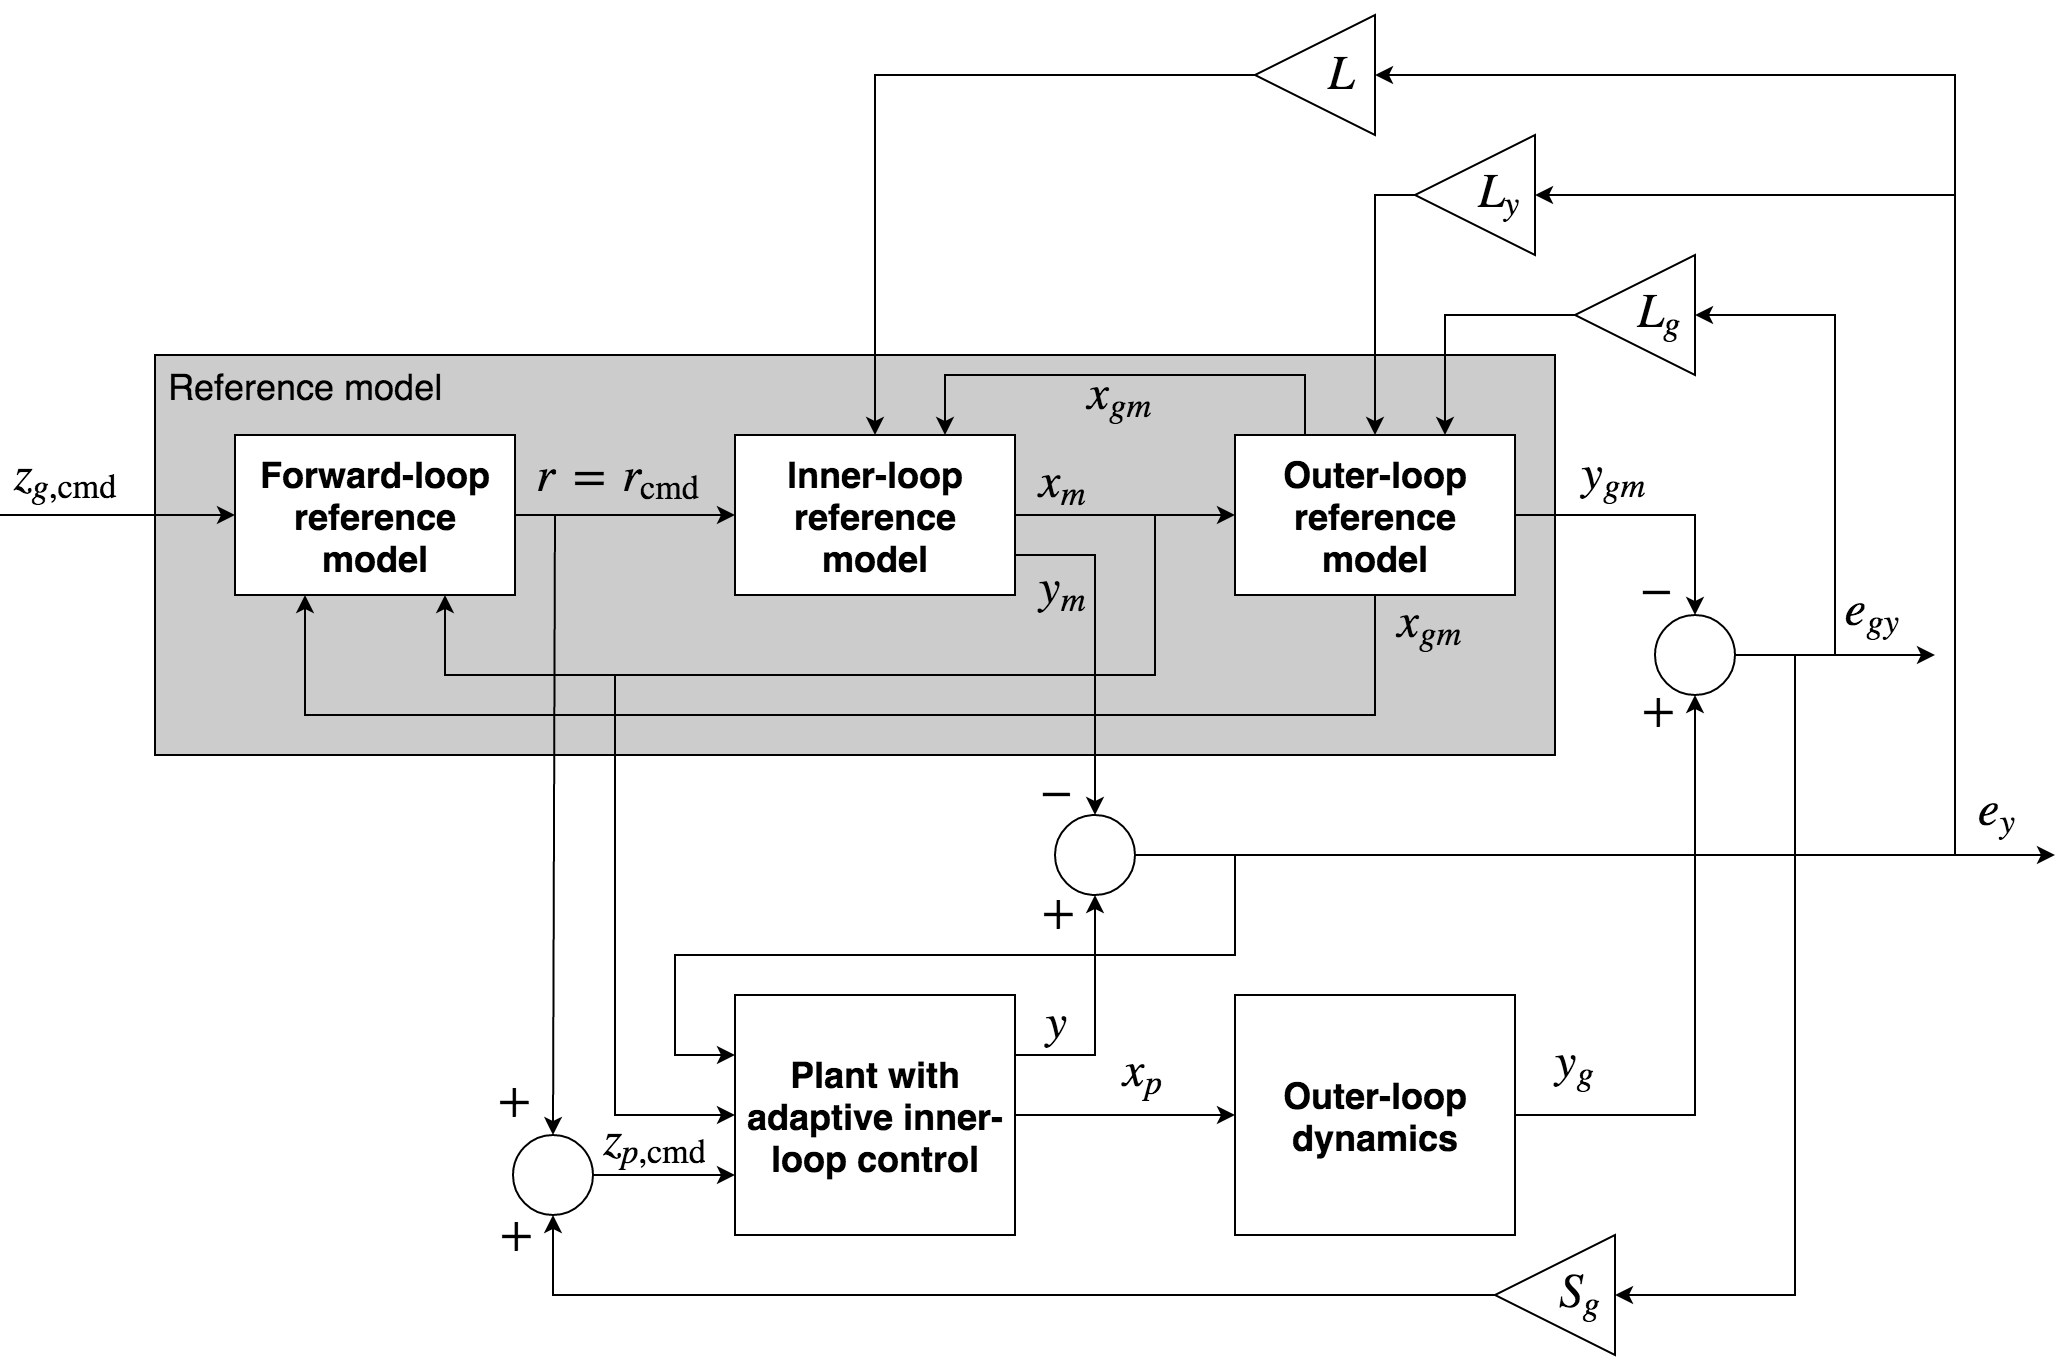
\includegraphics[width=6.5in]{\figurepath/innerAndOuterLoopDansOutputFeedback2.png}
    \vspace{-0.1in}
    \caption{Complete integrated inner and outer-loop design block diagram.\label{fig.innerAndOuterLoopDansOutputFeedback}}
  \end{center}
\end{figure}

\begin{figure}[H]
  \begin{center}
    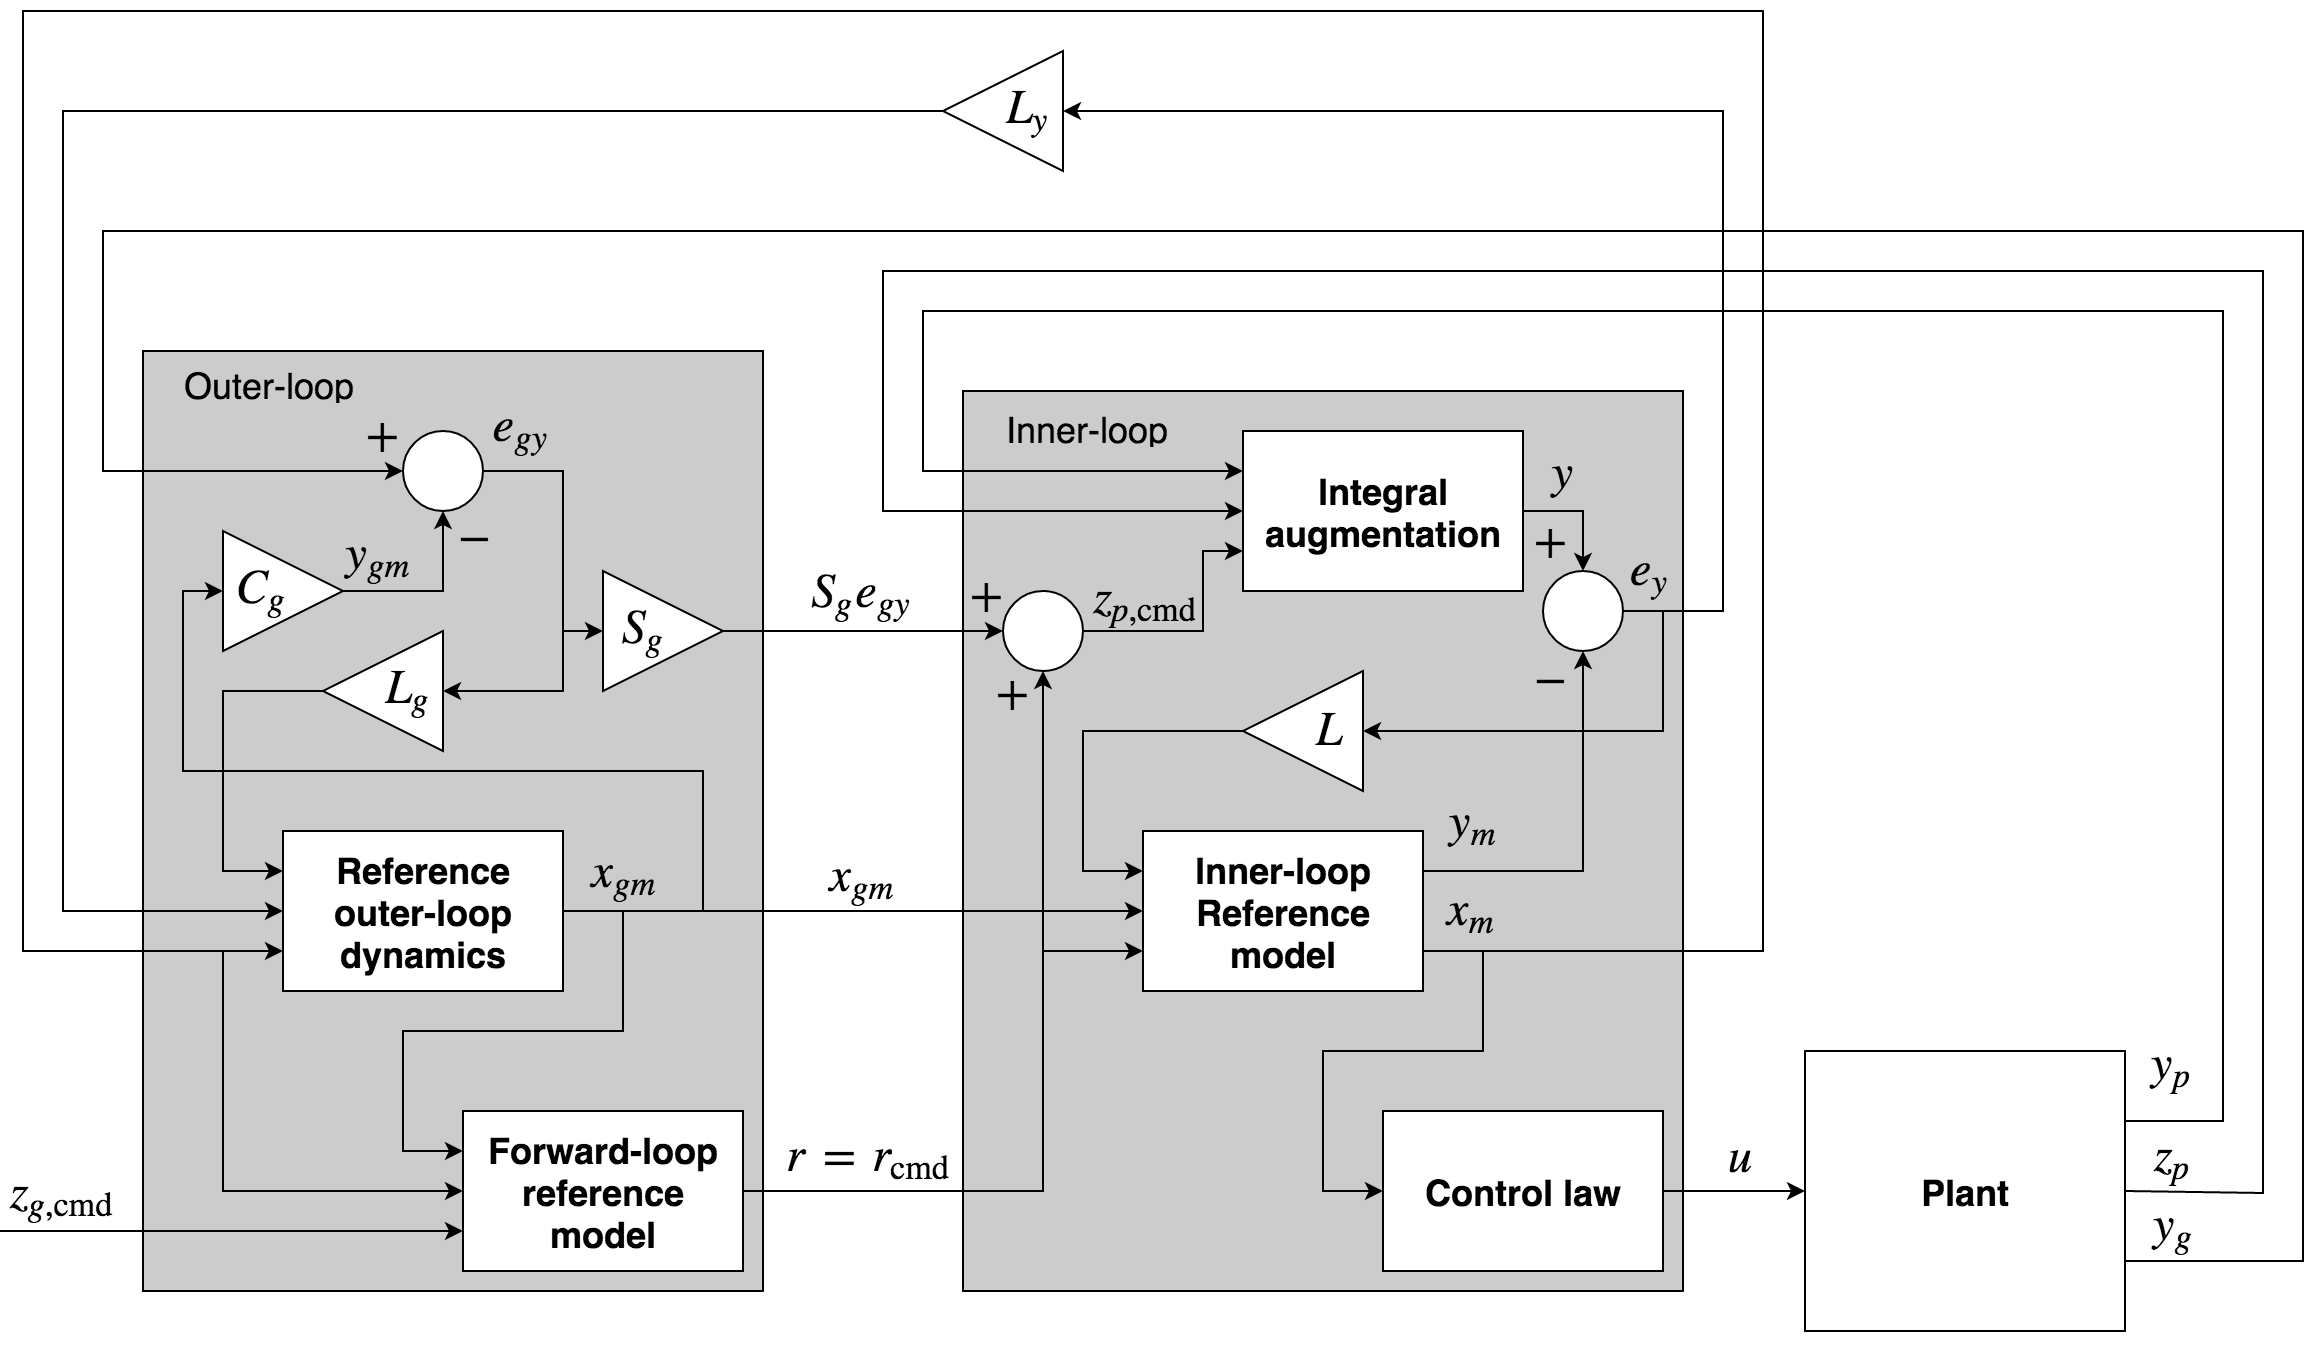
\includegraphics[width=6.5in]{\figurepath/innerAndOuterLoopExplicit.png}
    \vspace{-0.1in}
    \caption{Complete integrated inner and outer-loop design block diagram.\label{fig.innerAndOuterLoopExplicit}}
  \end{center}
\end{figure}

In the most simple form, the block diagram in Figure~\ref{fig.innerAndOuterLoopExplicit} can be represented using the block diagram in Figure~\ref{fig.simpleBlockWithoutLimiter} where $x(t)$ represents the feedback of the plant and inner-loop reference model outputs and contains $y_{g}(t)$, $e_{y}(t)$, and $x_{m}(t)$.
The signal $e(t)$ contains the outer-loop error $e_{gs}(t)$ and the outer-loop reference model state $x_{gm}(t)$.

\begin{figure}[H]
  \begin{center}
    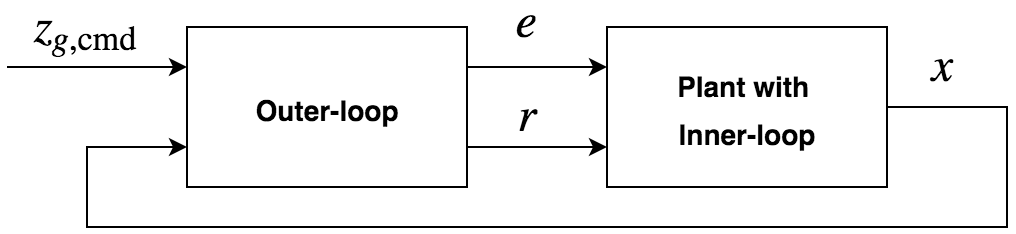
\includegraphics[width=4.5in]{\figurepath/simpleBlockWithoutLimiter.png}
    \vspace{-0.1in}
    \caption{Simplified inner and outer-loop block diagram.\label{fig.simpleBlockWithoutLimiter}}
  \end{center}
\end{figure}

The above sections have presented the inner-loop control design and the outer-loop architecture including the forward-loop reference model.
Combining the inner-loop error dynamics in\ \eqref{eqn.errordynamics4} with the outer-loop error dynamics in\ \eqref{eqn.outerlooperrordynamics} with $z_{p,\text{cmd}}(t)$ given by\ \eqref{eqn.zpcmd} and\ \eqref{eqn.egs} the following inner and outer-loop error dynamics are obtained
\begin{equation}
  \label{eqn.innerAndOuterLoopErrorDynamics1}
  \begin{split}
    \dot{e}_{x}(t)
    &=
    \bigr(A+LC+B\Psi^{\top}\bigr)e_{x}(t) + B\Lambda\widetilde{\Theta}^{\top}(t)x_{m}(t) + \bigr(B_{\text{cmd}}S_{g}C_{g} + B_{d}\bigr)e_{g}(t) \\
    \dot{e}_{g}(t)
    &=
    \bigr(A_{g} + L_{g}C_{g}\bigr)e_{g}(t) + \bigr(B_{g} + L_{y}C\bigr)e_{x}(t) \\
  \end{split}
\end{equation}
The CRM feedback gains $L_{y}$, $L_{g}$, and $S_{g}$ in\ \eqref{eqn.innerAndOuterLoopErrorDynamics1} need to be selected to guarantee global stability of the closed-loop system.
Looking at these error dynamics provied a cue as to how stability may be achieved, with $L_{g}$ being used to stabilize the outer-loop error dynamics, and $S_{g}$ and $L_{y}$ used to cancel the error cross-coupling terms.
By selecting these outer-loop reference model gains in this way, the error dynamics are essentially reduced to standard adaptive error dynamics on the inner-loop, and stable outer-loop error dynamics.
The specific requirements for stability of the error dynamics in\ \eqref{eqn.innerAndOuterLoopErrorDynamics1} and the resulting conditions leading to the solutions for $S_{g}$, $L_{g}$ and $L_{y}$ are provided in the following subsection.

\subsection{Conditions for Stability}

The complete control architecture is specified by the plant and reference model\ \eqref{eqn.plantAndCompactReferenceModel}, inner-loop command specified by\ \eqref{eqn.zpcmd} and\ \eqref{eqn.egs}, control input\ \eqref{eqn.u}, and update law in\ \eqref{eqn.updatelaw}.
All that remains to complete the control design is to specify solutions to $L_{y}$, $L_{g}$, and $S_{g}$ such that the closed-loop system is stable and the control goal of command tracking is satisfied.
In order to prove stability of the closed-loop system, the matrices $L_{y}$, $S_{g}$, and $P_{g}=P_{g}^{\top}>0$ need to be found satisfying the following condition
\begin{equation}
  \label{eqn.condition1}
  (B_{g}+L_{y}C)^{\top}P_{g} + P_{x}B_{\text{cmd}}S_{g}C_{g} + B_{d} = 0
\end{equation}
where $L_{g}$ must be picked together with $P_{g}$ so that, in addition, the following Lyapunov inequality is satisfied
  \begin{equation}
  \label{eqn.condition2}
  (A_{g}+L_{g}C_{g})^{\top}P_{g}+P_{g}(A_{g}+L_{g}C_{g}) < -Q_{g}
\end{equation}
where $Q_{g}=Q_{g}^{\top}>0$.
Together, the conditions in\ \eqref{eqn.condition1} and\ \eqref{eqn.condition2} can be combined, and the problem restated as: Find the matrices $L_{y}$, $S_{g}$, $L_{g}$ and $P_{g}$ that together satisfy the following conditions
\begin{align}
  \label{eqn.condition3a}
  (B_{g}+L_{y}C)^{\top}P_{g} + P_{x}B_{\text{cmd}}S_{g}C_{g} + B_{d} &= 0 \\
  \label{eqn.condition3b}
  (A_{g}+L_{g}C_{g})^{\top}P_{g}+P_{g}(A_{g}+L_{g}C_{g}) &< -Q_{g}
\end{align}
The condition in Eq.\ \eqref{eqn.condition3a} can be rearranged as
\begin{equation}
  \label{eqn.theEquation}
  C^{\top}L_{y}^{\top} = - P_{x}B_{\text{cmd}}S_{g}C_{g}P_{g}^{-1} - B_{g}^{\top} - B_{d}P_{g}^{-1}
\end{equation}
Examining the condition in\ \eqref{eqn.theEquation} it can be seen that the CRM gain $L_{y}^{\top}$ on the left hand side rotates and scale the columns of $C^{\top}$, but cannot do anything such that the columns of the matrix $C^{\top}L_{y}^{\top}$ are orthogonal to columns of $C^{\top}$.
This means that, in general, $L_{y}$ would not be enough to direct the columns of $C^{\top}$ so as to match the right hand side of\ \eqref{eqn.theEquation}.
Thus $S_{g}$ together with $P_{g}$ must be used to ensure the columns of the right hand side in are in the space spanned by the columns of $C^{\top}$.
That is, $S_{g}$ and $P_{g}$ must be selected such that when\ \eqref{eqn.theEquation} is left-multiplied by $M^{\top}$, that the quantity on the right hand side vanishes, where $M$ is the inner-loop measured output annihilator matrix from\ \eqref{eqn.NB0CM0} that satisfies $CM=0$.
Left multiplying\ \eqref{eqn.theEquation} by $M^{\top}$ and substituting in the expression for $P_{x}$ from\ \eqref{eqn.Px} the following is obtained
\begin{equation}
  \label{eqn.makeMeZero}
  -M^{\top}N^{\top}XNB_{\text{cmd}}S_{g}C_{g}P_{g}^{-1} = M^{\top}(B_{g}^{\top} + B_{d}P_{g}^{-1})
\end{equation}
Furthermore, recall from Lemma~\ref{lem.elimination}, the Matrix Elimination Lemma, for an $L_{g}$ to exist satisfying\ \eqref{eqn.condition3b}, a $P_{g}$ must exist satisfying
\begin{equation}
  \label{eqn.reducedPgInequality}
  C_{g}^{\top\perp\top} (A_{g}^{\top}P_{g} + P_{g}A_{g}) C_{g}^{\top\perp} < 0
\end{equation}
Thus in order to find $L_{y}$, $S_{g}$, and $P_{g}$ satisfying\ \eqref{eqn.theEquation}, and thus\ \eqref{eqn.condition3a}, with the additional constraint that $P_{g}$ solves\ \eqref{eqn.reducedPgInequality}, thus guaranteeing an $L_{g}$ exists that solves\ \eqref{eqn.condition3b}, the matrices $P_{g}$ and $S_{g}$ must be found satisfying
\begin{align}
  \label{eqn.condition4a}
  -M^{\top}N^{\top}XNB_{\text{cmd}}S_{g}C_{g}P_{g}^{-1} &= M^{\top}(B_{g}^{\top} + B_{d}P_{g}^{-1}) \\
  \label{eqn.condition4b}
  C_{g}^{\top\perp\top} (A_{g}^{\top}P_{g} + P_{g}A_{g}) C_{g}^{\top\perp} &< 0
\end{align}
If $S_{g}$ and $P_{g}$ exist satisfying\ \eqref{eqn.condition4a} and\ \eqref{eqn.condition4b}, then the solution to the outer-loop control problem exists.
Once solutions $S_{g}$ and $P_{g}$ are found analytically, an $L_{g}$ satisfying\ \eqref{eqn.condition3b} is guaranteed to exist, which can be simply found it by solving\ \eqref{eqn.condition3b} numerically, as was done to obtain $L$ in the inner-loop design in Chapter~\ref{ch.innerLoop}.
With the solutions $S_{g}$ and $P_{g}$, the solution $L_{y}$ from\ \eqref{eqn.theEquation} is calculated.
So the problem that remains is to find $S_{g}$ and $P_{g}$ satisfying\ \eqref{eqn.condition4a} and\ \eqref{eqn.condition4b}.

\begin{rem-dan}
  If the requirement that the inequality in\ \eqref{eqn.condition3b} be strict is relaxed, then the condition given by\ \eqref{eqn.condition4b} is changed so as not to be a strict inequality either.
\end{rem-dan}

The existence of solutions to\ \eqref{eqn.condition4a} is dependent on the sizes of the matrices.
Based on these different sizes will affect how\ \eqref{eqn.condition4a} is manipulated to get it in a form which can be solved.

\subsubsection{Case I:~$n-p=n_{ep}$}

This case corresponds to the number of inner-loop regulated outputs $n_{ep}$, being equal to the number of unmeasured inner-loop states, given by $n-p$.
In this case, $M^{\top}N^{\top}XNB_{\text{cmd}}$ in\ \eqref{eqn.condition4a} is square, and full rank as specified in Remark~\ref{rem.X12FullRank}, so left-multiply\ \eqref{eqn.condition4a} by $(M^{\top}N^{\top}XNB_{\text{cmd}})^{-1}$ and right-multiply by $P_{g}$ to obtain
\begin{equation}
  \label{eqn.SgCg}
  S_{g}C_{g} = - (M^{\top}N^{\top}XNB_{\text{cmd}})^{-1}M^{\top}(B_{g}^{\top}+B_{d}P_{g}^{-1})P_{g}
\end{equation}
It can be seen from\ \eqref{eqn.SgCg} that $S_{g}$ can only rotate the vectors that make up the rows of $C_{g}$ to other directions within their span.
Thus, it is necessary to make sure that the right hand side of\ \eqref{eqn.SgCg} lies in the same span as the rows of $C_{g}$, then $S_{g}$ can be used to rotate them as required.
For the right hand side to be in the same span as the rows of $C_{g}$, it has to have the same nullspace.
That is, if\ \eqref{eqn.SgCg} is multiplied on the right hand side by $C_{g}^{\top\perp}$ the resulting quantity must be zero.
Thus the goal is to find $P_{g}$ satisfying the following
\begin{equation}
  \label{eqn.PgMustSatisfyCaseI}
  (M^{\top}N^{\top}XNB_{\text{cmd}})^{-1}M^{\top}(B_{g}^{\top}+B_{d}P_{g}^{-1})P_{g}C_{g}^{\top\perp} = 0
\end{equation}
But since $M^{\top}N^{\top}XNB_{\text{cmd}}$ is square and full rank, finding $P_{g}$ satisfying\ \eqref{eqn.PgMustSatisfyCaseI} is equivalent to finding $P_{g}$ satisfying the following equation
\begin{equation}
  \label{eqn.AXBCcase1}
  M^{\top}B_{g}^{\top}P_{g}C_{g}^{\top\perp} = -M^{\top}B_{d}C_{g}^{\top\perp}
\end{equation}
with $M^{\top}B_{g}^{\top}\in\mathbb{R}^{n-p\times n_{g}}$ and $C_{g}^{\top\perp}\in\mathbb{R}^{n_{g}\times n_{g}-p_{g}}$.
Since $C_{g}$ is always wide, $S_{g}$ from\ \eqref{eqn.SgCg} can be solved for using a right inverse of $C_{g}$ to get
\begin{equation}
  \label{eqn.SgCaseI}
  S_{g} = - (M^{\top}N^{\top}XNB_{\text{cmd}})^{-1}M^{\top}(B_{g}^{\top}+B_{d}P_{g}^{-1})P_{g}C_{g}^{-1_{\text{right}}}
\end{equation}

\subsubsection{Case II:~$n-p<n_{ep}$}

This case corresponds to the number of inner-loop regulated outputs $n_{ep}$, being greater than the number of unmeasured inner-loop states, given by $n-p$.
In this case $M^{\top}N^{\top}XNB_{\text{cmd}}$ in\ \eqref{eqn.condition4a} is wide.
A right inverse is used to simplify\ \eqref{eqn.condition4a} as
\begin{equation*}
  S_{g}C_{g}
  =
  -(M^{\top}N^{\top}XNB_{\text{cmd}})^{-1_{\text{right}}}M^{\top}(B_{g}^{\top}+B_{d}P_{g}^{-1})P_{g}
\end{equation*}
As in Case I, $S_{g}$ can only match the right hand side in the span of $C_{g}$, so need to make sure that the right hand side is within the span of $C_{g}$.
So $P_{g}$ must satisfy
\begin{equation}
  \label{eqn.PgMustSatisfyCaseII}
  (M^{\top}N^{\top}XNB_{\text{cmd}})^{-1_{\text{right}}}M^{\top}(B_{g}^{\top}+B_{d}P_{g}^{-1})P_{g}C_{g}^{\top\perp} = 0
\end{equation}
But because $(M^{\top}N^{\top}XNB_{\text{cmd}})^{-1_{\text{right}}}$ is tall and full rank, finding $P_{g}$ satisfying\ \eqref{eqn.PgMustSatisfyCaseII} is equivalent to finding $P_{g}$ satisfying the following equation
\begin{equation}
  \label{eqn.AXBCcase2}
  M^{\top}B_{g}^{\top}P_{g}C_{g}^{\top\perp} = - M^{\top}B_{d}C_{g}^{\top\perp}
\end{equation}
Once $P_{g}$ satisfying\ \eqref{eqn.AXBCcase2} is found, $S_{g}$ is determined by
\begin{equation}
  \label{eqn.SgCaseII}
  S_{g} = - (M^{\top}N^{\top}XNB_{\text{cmd}})^{-1_{\text{right}}}M^{\top}(B_{g}^{\top}+B_{d}P_{g}^{-1})P_{g}C_{g}^{-1_{\text{right}}}
\end{equation}

\subsubsection{Case III:~$n-p>n_{ep}$}

This case corresponds to the number of inner-loop regulated outputs $n_{ep}$, being less than the number of unmeasured inner-loop states, given by $n-p$.
In this case $M^{\top}N^{\top}XNB_{\text{cmd}}$ in\ \eqref{eqn.condition4a} is tall, so $S_{g}$ doesn't have the degrees of freedom to satisfy\ \eqref{eqn.condition4a}.

The conditions for the existence of $S_{g}$ and $P_{g}$ exist satisfying\ \eqref{eqn.condition4a} and\ \eqref{eqn.condition4b} is stated in the following theorem.

\begin{thm-dan}\label{thm.existenceOuterLoop}
  For the existence of $S_{g}$ and $P_{g}$ satisfying\ \eqref{eqn.condition4a} and\ \eqref{eqn.condition4b} for a stable outer-loop controller, the plant must satisfy $n-p\leq n_{ep}$, $n-p<n_{g}$, as well as the following inequality
  \begin{equation}
    \label{eqn.outerLoopTheoremInequality}
    C_{g}^{\top\perp\top}A_{g}^{\top}(B_{g}M)^{\perp}\bigr(C_{g}^{\top\perp\top}(B_{g}M)^{\perp}\bigr)^{-1_{\textnormal{right}}}
    <0
  \end{equation}
\end{thm-dan}

\begin{proof-dan}
  Finding $S_{g}$ and $P_{g}$ satisfying\ \eqref{eqn.condition4a} involves first manipulating\ \eqref{eqn.condition4a} by selecting $P_{g}$ to ensure that $S_{g}$, which acts through the rows of $C_{g}$, will be sufficient to satisfy\ \eqref{eqn.condition4a}.
  This results in a finding the set of all $P_{g}=P_{g}^{\top}>0$ which satisfy $\Pi_{A}P_{g}\Pi_{B}=\Pi_{C}$, where $\Pi_{A}$, $\Pi_{B}$, and $\Pi_{C}$ are matrices which depend on the state-space plant matrices.
  Finding $P_{g}$ involves using a generalized singular value decomposition, and fixes certain elements of $P_{g}$ based on $\Pi_{A}$, $\Pi_{B}$, and $\Pi_{C}$.
  Then, from this set of $P_{g}$, those which also satisfy\ \eqref{eqn.condition4b} are found.
  This involves substituting the form of $P_{g}$ into\ \eqref{eqn.condition4b} and manipulating to obtain\ \eqref{eqn.outerLoopTheoremInequality}.
  These steps are outlined in detail in the following sections.
\end{proof-dan}

\begin{rem-dan}
  The control solution is still possible when the inequality in\ \eqref{eqn.outerLoopTheoremInequality} is not strict, which results in\ \eqref{eqn.condition4b} not being strict as well.
  The implications this has on tracking are discussed following the stability proof, but it is noted that outer-loop command tracking is still achieved as desired.
\end{rem-dan}

\begin{rem-dan}
  For the existence of a stable outer loop as described in Theorem~\ref{thm.existenceOuterLoop} for the case when $n-p\geq n_{g}$, a solution is still possible, but requires additional constraints to be satisfied.
  See Appendix~\ref{app.proofs}.
\end{rem-dan}

\section{Solving $P_{g}$: Symmetric Solutions to the Matrix Equation $\Pi_{A}P_{g}\Pi_{B}=\Pi_{C}$}

Solving for $P_{g}$ in\ \eqref{eqn.AXBCcase1} and\ \eqref{eqn.AXBCcase2} for $P_{g}=P_{g}^{\top}>0$ are in the form $\Pi_{A}P_{g}\Pi_{B}=\Pi_{C}$, and $P_{g}$ must also satisfy\ \eqref{eqn.condition4b}.
In the two cases above, the matrices $\Pi_{A}$, $\Pi_{B}$, and $\Pi_{C}$ in\ \eqref{eqn.AXBCcase1} and\ \eqref{eqn.AXBCcase2} are given by
\begin{equation}
  \label{eqn.AXBandCCaseI}
  \begin{split}
    \Pi_{A} &= M^{\top}B_{g}^{\top} \\
    \Pi_{B} &= C_{g}^{\top\perp} \\
    \Pi_{C} &= -M^{\top}B_{d}C_{g}^{\top\perp} \\
  \end{split}
\end{equation}
where $\Pi_{A}\in\mathbb{R}^{n-p\times n_{g}}$, $P_{g}\in\mathbb{R}^{n_{g}\times n_{g}}$, $\Pi_{B}\in\mathbb{R}^{n_{g}\times n_{g}-p_{g}}$ and $\Pi_{C}\in\mathbb{R}^{n-p\times n_{g}-p_{g}}$.
Using the definitions in\ \eqref{eqn.AXBandCCaseI}, the inequality\ \eqref{eqn.condition4b} is rewritten and the problem once again restated as: Find $P_{g}=P_{g}^{\top}>0$ satisfying
\begin{align}
  \label{eqn.PiAPgPiBPiC}
  \Pi_{A}P_{g}\Pi_{B} &= \Pi_{C} \\
  \label{eqn.condition4bCaseI}
  \Pi_{B}^{\top} (A_{g}^{\top}P_{g} + P_{g}A_{g}) \Pi_{B} &< 0
\end{align}
where $\Pi_{A}$, $\Pi_{B}$, and $\Pi_{C}$ are defined in\ \eqref{eqn.AXBandCCaseI}.

\subsection{A Generalized Singular Value Decomposition}

Determining solutions $P_{g}$ to Eq.\ \eqref{eqn.PiAPgPiBPiC} involves first decompose the matrices $\Pi_{A}$ and $\Pi_{B}$ in\ \eqref{eqn.AXBandCCaseI} using a generalized singular value decomposition (GSVD)\ \cite{golub.matrix.1996,dai.symmetric.1996,paige.towardsgsvd.1981,hua.symmetric.1990} as follows
\begin{equation}
  \label{eqn.AandBGSVD}
  \begin{split}
    \Pi_{A} &= U\Sigma_{A}P \\
    \Pi_{B}^{\top} &= V\Sigma_{B}P
  \end{split}
\end{equation}
where $U\in\mathbb{R}^{n-p\times n-p}$ and $V\in\mathbb{R}^{n_{g}-p_{g}\times n_{g}-p_{g}}$, $P\in\mathbb{R}^{n_{g}\times n_{g}}$, and $\Sigma_{A}\in\mathbb{R}^{n-p\times n_{g}}$ and $\Sigma_{B}\in\mathbb{R}^{n_{g}-p_{g}\times n_{g}}$.
This decomposition is provided in detail in the above references, and described here for the case where the rank of the following matrix is full.
\begin{equation}
  \label{eqn.gsvdmatrixfullrank}
  \begin{bmatrix}
    \Pi_{A} \\
    \Pi_{B}^{\top}
  \end{bmatrix}
\end{equation}
As the matrices $\Pi_{A}$ and $\Pi_{B}$ in\ \eqref{eqn.gsvdmatrixfullrank} essentially capture the unmeasurable system outputs, the requirement that\ \eqref{eqn.gsvdmatrixfullrank} be full rank can be easily satisfied for most systems by appropriate selection of the sensors used.
A simplified way this full rank condition can be interpreted is that if the system in\ \eqref{eqn.wholeSystemUncertain} is not observable using only the inner-loop output $y_{p}(t)$, then using outer-loop measurements that are simply pure integrations of the inner-loop measurements will not make the system observable.
Instead, the outer-loop measurements must contain additional information about the outer-loop states.
The matrices describing the decomposition in Eq.\ \eqref{eqn.AandBGSVD} when\ \eqref{eqn.gsvdmatrixfullrank} is full rank are given by
\begin{equation}
  \label{eqn.SigmaASigmaB}
  \begin{split}
    \Sigma_{A}
    &=
    \begin{bmatrix}
      I_{n-p\times n-p} & 0_{n-p\times n_{g}-p_{g}} & 0_{n-p\times p-n+p_{g}}
    \end{bmatrix} \\
    \Sigma_{B}
    &=
    \begin{bmatrix}
      0_{n_{g}-p_{g}\times n-p} & I_{n_{g}-p_{g}\times n_{g}-p_{g}} & 0_{n_{g}-p_{g}\times p-n+p_{g}}
    \end{bmatrix} \\
  \end{split}
\end{equation}
and
\begin{equation}
  \label{eqn.P}
  P = P_{\Lambda}
  \begin{bmatrix}
    \Pi_{A} \\
    \Pi_{B}^{\top} \\
    \begin{bmatrix}
      \Pi_{A}^{\top} & \Pi_{B}
    \end{bmatrix}^{\perp\top} \\
  \end{bmatrix}
\end{equation}
where $P_{\Lambda}$ is an arbitrary block diagonal matrix, with full rank, given by
\begin{equation}
  \label{eqn.PLambda}
  P_{\Lambda} =
  \begin{bmatrix}
    P_{A} & 0 & 0 \\
    0 & P_{B} & 0 \\
    0 & 0 & P_{N}
  \end{bmatrix}
\end{equation}
where $P_{A}\in\mathbb{R}^{n-p\times n-p}$, $P_{B}\in\mathbb{R}^{n_{g}-p_{g}\times n_{g}-p_{g}}$, and $P_{N}\in\mathbb{R}^{p+p_{g}-n \times p+p_{g}-n}$ are each matrices of full rank.
Substituting\ \eqref{eqn.PLambda} into\ \eqref{eqn.P} gives
\begin{equation}
  \label{eqn.PP}
  P
  =
  \begin{bmatrix}
    P_{A}\Pi_{A} \\
    P_{B}\Pi_{B}^{\top} \\
    P_{N}
    \begin{bmatrix}
      \Pi_{A}^{\top} & \Pi_{B}
    \end{bmatrix}^{\perp\top} \\
  \end{bmatrix}
\end{equation}
Select $U$ and $V$ in\ \eqref{eqn.AandBGSVD} as
\begin{equation*}
  \begin{split}
    U &= P_{A}^{-1} \\
    V &= P_{B}^{-1}
  \end{split}
\end{equation*}
ensures that the decomposition\ \eqref{eqn.AandBGSVD} holds.

\subsection{Satisfying $\Pi_{A}P_{g}\Pi_{B}=\Pi_{C}$ with $P_{g}=P_{g}^{\top}>0$}

With $\Pi_{A}$ and $\Pi_{B}$ decomposed as in\ \eqref{eqn.AandBGSVD} and plugging these expressions into the equation $\Pi_{A}P_{g}\Pi_{B}=\Pi_{C}$ gives
\begin{equation}
  \label{eqn.USigmaAPXPSigmaBVC}
  U\Sigma_{A}PP_{g}P^{\top}\Sigma_{B}^{\top}V^{\top} = \Pi_{C}
\end{equation}
Propose the following solution $P_{g}$ to\ \eqref{eqn.USigmaAPXPSigmaBVC}
\begin{equation}
  \label{eqn.Pg}
  P_{g} = P^{-1}X_{D}P^{-\top}
\end{equation}
where $X_{D}=X_{D}^{\top}>0$ ensures that $P_{g}=P_{g}^{\top}>0$.
Plugging the form of $P_{g}$ from\ \eqref{eqn.Pg} into\ \eqref{eqn.USigmaAPXPSigmaBVC} results in
\begin{equation*}
  U\Sigma_{A}PP^{-1}X_{D}P^{-\top} P^{\top}\Sigma_{B}^{\top}V^{\top}
  =
  \Pi_{C}
\end{equation*}
which can be simplified as
\begin{equation}
  \label{eqn.USigmaAXDSigmaBV}
  U\Sigma_{A}X_{D}\Sigma_{B}^{\top}V^{\top} = \Pi_{C}
\end{equation}
The matrix $X_{D}=X_{D}^{\top}>0$ is written as
\begin{equation}
  \label{eqn.XD}
  X_{D} =
  \begin{bmatrix}
    X_{D11} & X_{D12} & X_{D13} \\
    X_{D12}^{\top} & X_{D22} & X_{D23} \\
    X_{D13}^{\top} & X_{D23}^{\top} & X_{D33} \\
  \end{bmatrix}
\end{equation}
where $X_{D11}\in\mathbb{R}^{n-p\times n-p}$, $X_{D12}\in\mathbb{R}^{n-p\times n_{g}-p_{g}}$, $X_{D13}\in\mathbb{R}^{n-p\times p-n+p_{g}}$, $X_{D22}\in\mathbb{R}^{n_{g}-p_{g}\times n_{g}-p_{g}}$, $X_{D23}\in\mathbb{R}^{n_{g}-p_{g}\times p-n+p_{g}}$, and $X_{D33}\in\mathbb{R}^{p-n+p_{g}\times p-n+p_{g}}$.
Plugging in the form of $X_{D}$ from\ \eqref{eqn.XD} and $\Sigma_{A}$ and $\Sigma_{B}$ from\ \eqref{eqn.SigmaASigmaB} into\ \eqref{eqn.USigmaAXDSigmaBV} gives
\begin{equation*}
  U
  \begin{bmatrix}
    I & 0 & 0
  \end{bmatrix}
  \begin{bmatrix}
    X_{D11} & X_{D12} & X_{D13} \\
    X_{D12}^{\top} & X_{D22} & X_{D23} \\
    X_{D13}^{\top} & X_{D23}^{\top} & X_{D33} \\
  \end{bmatrix}
  \begin{bmatrix}
    0 \\
    I \\
    0
  \end{bmatrix}
  V^{\top}
  = \Pi_{C}
\end{equation*}
which simplifies to
\begin{equation*}
  U
  X_{D12}
  V^{\top}
  = \Pi_{C}
\end{equation*}
Solve for $X_{D12}$ as
\begin{equation}
  \label{eqn.XD12}
  \begin{split}
    X_{D12}
    &= U^{-1}CV^{-\top} \\
    &= P_{A}\Pi_{C}P_{B}^{\top}
  \end{split}
\end{equation}
The choice of $X_{D12}$ in\ \eqref{eqn.XD12}, ensures that $P_{g}$ given by\ \eqref{eqn.Pg} with $X_{D}$ given by\ \eqref{eqn.XD} satisfies the equation $\Pi_{A}P_{g}\Pi_{B}=\Pi_{C}$.
However, the remaining degrees of freedom in $X_{D}$ must be selected to ensure also that $P_{g}>0$, and that $P_{g}$ also satisfies the inequality\ \eqref{eqn.condition4bCaseI}.

\subsection{Satisfying $\Pi_{B}^{\top} (A_{g}^{\top}P_{g} + P_{g}A_{g}) \Pi_{B} < 0$}

With the form of $P_{g}$ given by\ \eqref{eqn.Pg} dependent on $X_{D}$ given in\ \eqref{eqn.XD} with $X_{D12}$ given in\ \eqref{eqn.XD12} and $P$ given in\ \eqref{eqn.PP}, the goal now is to find the remaining elements of $X_{D}$ so that the resulting $P_{g}$ satisfies the inequality\ \eqref{eqn.condition4bCaseI} and ensures $P_{g}>0$.
Plugging the form of $X$ from\ \eqref{eqn.Pg} into the matrix elimination lemma inequality from\ \eqref{eqn.condition4bCaseI} gives
\begin{equation}
  \label{eqn.condition4bCaseI2}
  \Pi_{B}^{\top}(A_{g}^{\top}P^{-1}X_{D}P^{-\top} + P^{-1}X_{D}P^{-\top}A_{g})\Pi_{B} < 0
\end{equation}
rearrange as
\begin{equation}
  \label{eqn.condition4bCaseI3}
  \Pi_{B}^{\top}P^{-1} (PA_{g}^{\top}P^{-1}X_{D} + X_{D}P^{-\top}A_{g}P^{\top}) P^{-\top}\Pi_{B} < 0
\end{equation}
To try to find an analytical expression for $P^{-1}$ given the expression for $P$, its inverse $P^{-1}$ must satisfy
\begin{equation}
  \label{eqn.PexpandedTimesPinv}
  \begin{bmatrix}
    P_{A}\Pi_{A} \\
    P_{B}\Pi_{B}^{\top} \\
    P_{N}
    \begin{bmatrix}
      \Pi_{A}^{\top} & \Pi_{B}
    \end{bmatrix}^{\perp\top} \\
  \end{bmatrix}
  P^{-1}
  =
  \begin{bmatrix}
  I & 0 & 0 \\
  0 & I & 0 \\
  0 & 0 & I \\
  \end{bmatrix}
\end{equation}
It can be seen from this that
\begin{equation}
  P_{B}\Pi_{B}^{\top}P^{-1} =
  \begin{bmatrix}
    0 & I & 0
  \end{bmatrix}
\end{equation}
from which it can be seen
\begin{equation}
  \label{eqn.BTPinv}
  \Pi_{B}^{\top}P^{-1} =
  \begin{bmatrix}
    0 & P_{B}^{-1} & 0
  \end{bmatrix}
\end{equation}
Using\ \eqref{eqn.BTPinv}, the inequality\ \eqref{eqn.condition4bCaseI3} becomes
\begin{equation}
  \label{eqn.condition4bCaseI4}
  \begin{bmatrix}
    0 & P_{B}^{-1} & 0
  \end{bmatrix}
  (PA_{g}^{\top}P^{-1}X_{D} + X_{D}P^{-\top}A_{g}P^{\top})
  \begin{bmatrix}
    0 \\
    P_{B}^{-\top} \\
    0 \\
  \end{bmatrix}
  < 0
\end{equation}
Defining $\bar{P}$ as
\begin{equation}
  \label{eqn.Pbar}
  \bar{P} = PA_{g}^{\top}P^{-1}
\end{equation}
the inequality\ \eqref{eqn.condition4bCaseI4} can be written as
\begin{equation}
  \label{eqn.condition4bCaseI5}
  \begin{bmatrix}
    0 & P_{B}^{-1} & 0
  \end{bmatrix}
  (\bar{P}X_{D} + X_{D}\bar{P}^{\top})
  \begin{bmatrix}
    0 \\
    P_{B}^{-\top} \\
    0 \\
  \end{bmatrix}
  < 0
\end{equation}
It is now necessary to examine the structure of the matrix $\bar{P}$ in the inequality\ \eqref{eqn.condition4bCaseI5}, which requires an expression for $P^{-1}$ so as to determine $\bar{P}$ as given by\ \eqref{eqn.Pbar}.
Given $P$ in\ \eqref{eqn.PP}, its inverse $P^{-1}$ must obviously satisfy $PP^{-1}=I$ as in\ \eqref{eqn.PexpandedTimesPinv}.
Examining\ \eqref{eqn.PexpandedTimesPinv} it can be seen that the columns of $P^{-1}$ are given by
\begin{equation}
  \label{eqn.PPinv}
  P^{-1} =
  \begin{bmatrix}
    \Pi_{B}^{\perp}\bigr(P_{A}\Pi_{A}\Pi_{B}^{\perp}\bigr)^{-1_{\text{right}}}
    &
    \Pi_{A}^{\top\perp}\bigr(P_{B}\Pi_{B}^{\top}\Pi_{A}^{\top\perp}\bigr)^{-1_{\text{right}}}
    &
    \times
  \end{bmatrix}
\end{equation}
where $\times$ indicates a column of $P^{-1}$ which is to remain unspecified.
Expanding $P$ and $P^{-1}$, the requirement that $PP^{-1}=I$ requires the following conditions be satisfied
\begin{equation}
  \label{eqn.firstColumnOfPinv}
  \begin{split}
    P_{A}\Pi_{A}\Pi_{B}^{\perp}\bigr(P_{A}\Pi_{A}\Pi_{B}^{\perp}\bigr)^{-1_{\text{right}}} &= I \\
    P_{B}\Pi_{B}^{\top}\Pi_{B}^{\perp}\bigr(P_{A}\Pi_{A}\Pi_{B}^{\perp}\bigr)^{-1_{\text{right}}} &= 0 \\
    P_{N}
    \begin{bmatrix}
      \Pi_{A}^{\top} & \Pi_{B}
    \end{bmatrix}^{\perp\top}
    \Pi_{B}^{\perp}\bigr(P_{A}\Pi_{A}\Pi_{B}^{\perp}\bigr)^{-1_{\text{right}}} &= 0
  \end{split}
\end{equation}
and
\begin{equation}
  \label{eqn.secondColumnOfPinv}
  \begin{split}
    P_{A}\Pi_{A}\Pi_{A}^{\top\perp}\bigr(P_{B}\Pi_{B}^{\top}\Pi_{A}^{\top\perp}\bigr)^{-1_{\text{right}}}
    &= 0 \\
    P_{B}\Pi_{B}^{\top}\Pi_{A}^{\top\perp}\bigr(P_{B}\Pi_{B}^{\top}\Pi_{A}^{\top\perp}\bigr)^{-1_{\text{right}}}
    &= I \\
    P_{N}
    \begin{bmatrix}
      \Pi_{A}^{\top} & \Pi_{B}
    \end{bmatrix}^{\perp\top}
    \Pi_{A}^{\top\perp}\bigr(P_{B}\Pi_{B}^{\top}\Pi_{A}^{\top\perp}\bigr)^{-1_{\text{right}}}
    &= 0 \\
  \end{split}
\end{equation}
The first two conditions in\ \eqref{eqn.firstColumnOfPinv} and\ \eqref{eqn.secondColumnOfPinv} are obvious, following from the definition of the right inverse, and properties of the annihilator matrices.
That each of the third conditions is true is less obvious, and is contained in Appendix~\ref{app.proofs}.
With $P^{-1}$ given by\ \eqref{eqn.PPinv}, $\bar{P}$ in\ \eqref{eqn.Pbar} can be written as
\begin{equation}
  \label{eqn.Pbar2}
  \bar{P} =
  \begin{bmatrix}
    P_{A}\Pi_{A} \\
    P_{B}\Pi_{B}^{\top} \\
    P_{N}
    \begin{bmatrix}
      \Pi_{A}^{\top} & \Pi_{B}
    \end{bmatrix}^{\perp\top} \\
  \end{bmatrix}
  A_{g}^{\top}
  \begin{bmatrix}
    \Pi_{B}^{\perp}\bigr(P_{A}\Pi_{A}\Pi_{B}^{\perp}\bigr)^{-1_{\text{right}}}
    &
    \Pi_{A}^{\top\perp}\bigr(P_{B}\Pi_{B}^{\top}\Pi_{A}^{\top\perp}\bigr)^{-1_{\text{right}}}
    &
    \times
  \end{bmatrix}
\end{equation}
where $\times$ in\ \eqref{eqn.Pbar2} again represents a column of $\bar{P}$ which remains unspecified.
$\bar{P}$ can also be partitioned into a block matrix given by
\begin{equation}
  \label{eqn.PbarPartitioned}
  \bar{P} =
  \begin{bmatrix}
    \bar{P}_{11} & \bar{P}_{12} & \bar{P}_{13} \\
    \bar{P}_{21} & \bar{P}_{22} & \bar{P}_{23}\\
    \bar{P}_{31} & \bar{P}_{32} & \bar{P}_{33}\\
  \end{bmatrix}
\end{equation}
where $P_{11}\in\mathbb{R}^{n-p \times n-p}$, $P_{12}\in\mathbb{R}^{n-p \times n_{g}-p_{g}}$, $P_{13}\in\mathbb{R}^{n-p \times p-n+p_{g}}$, $P_{21}\in\mathbb{R}^{n_{g}-p_{g} \times n-p}$, $P_{22}\in\mathbb{R}^{n_{g}-p_{g} \times n_{g}-p{g}}$, $P_{23}\in\mathbb{R}^{n_{g}-p_{g} \times p-n+p_{g}}$, $P_{31}\in\mathbb{R}^{p-n+p_{g} \times n-p}$, $P_{32}\in\mathbb{R}^{p-n+p_{g} \times n_{g}-p_{g}}$, and $P_{33}\in\mathbb{R}^{p-n+p_{g} \times p-n+p_{g}}$ with $\bar{P}_{21}$ and $\bar{P}_{22}$ given by
\begin{equation}
  \label{eqn.Pbar21andPbar22}
  \begin{split}
    \bar{P}_{21}
    &=
    P_{B}\Pi_{B}^{\top}A_{g}^{\top}\Pi_{B}^{\perp}
    \bigr(P_{A}\Pi_{A}\Pi_{B}^{\perp}\bigr)^{-1_{\text{right}}} \\
    \bar{P}_{22}
    &=
    P_{B}\Pi_{B}^{\top}A_{g}^{\top}\Pi_{A}^{\top\perp}\bigr(P_{B}\Pi_{B}^{\top}\Pi_{A}^{\top\perp}\bigr)^{-1_{\text{right}}}
  \end{split}
\end{equation}
The inequality in\ \eqref{eqn.condition4bCaseI5} with $\bar{P}$ given by\ \eqref{eqn.PbarPartitioned}, where $\bar{P}_{21}$ and $\bar{P}_{22}$ are given by\ \eqref{eqn.Pbar21andPbar22}, and $X_{D}$ given by\eqref{eqn.XD} must be satisfied by the selection of the remaining elements of $X_{D}$.
Plugging these expressions for $\bar{P}$ in\ \eqref{eqn.PbarPartitioned} and $X_{D}$ in\ \eqref{eqn.XD} into the inequality in\ \eqref{eqn.condition4bCaseI5} gives
\begin{equation}
  \label{eqn.condition4bCaseI6}
  \begin{split}
    \begin{bmatrix}
      0 & P_{B}^{-1} & 0
    \end{bmatrix}
    &
    \left(
    \begin{bmatrix}
      \bar{P}_{11} & \bar{P}_{12} & \bar{P}_{13} \\
      \bar{P}_{21} & \bar{P}_{22} & \bar{P}_{23}\\
      \bar{P}_{31} & \bar{P}_{32} & \bar{P}_{33}\\
    \end{bmatrix}
    \right.
    \begin{bmatrix}
      X_{D11} & X_{D12} & X_{D13} \\
      X_{D12}^{\top} & X_{D22} & X_{D23} \\
      X_{D13}^{\top} & X_{D23}^{\top} & X_{D33} \\
    \end{bmatrix} \\
    &+
    \begin{bmatrix}
      X_{D11} & X_{D12} & X_{D13} \\
      X_{D12}^{\top} & X_{D22} & X_{D23} \\
      X_{D13}^{\top} & X_{D23}^{\top} & X_{D33} \\
    \end{bmatrix}
    \left.
    \begin{bmatrix}
      \bar{P}_{11}^{\top} & \bar{P}_{21}^{\top} & \bar{P}_{31}^{\top} \\
      \bar{P}_{12}^{\top} & \bar{P}_{22}^{\top} & \bar{P}_{32}^{\top}\\
      \bar{P}_{13}^{\top} & \bar{P}_{23}^{\top} & \bar{P}_{33}^{\top}\\
    \end{bmatrix}
    \right)
    \begin{bmatrix}
      0 \\
      P_{B}^{-\top} \\
      0 \\
    \end{bmatrix}
    < 0
  \end{split}
\end{equation}
which is equivalent to
\begin{equation}
  \label{eqn.condition4bCaseI7}
  \bar{P}_{21}X_{D12} + \bar{P}_{22}X_{D22} + \bar{P}_{23}X_{D23}^{\top}
  +
  X_{D12}^{\top}\bar{P}_{21}^{\top} + X_{D22}\bar{P}_{22}^{\top} + X_{D23}^{\top}\bar{P}_{23}^{\top}
  < 0
\end{equation}
The $P_{B}$ terms in\ \eqref{eqn.condition4bCaseI6} can be dropped, as they are full rank matrices, and thus have no influence on the satisfaction of the inequality.
$X_{D12}$ in\ \eqref{eqn.condition4bCaseI7} is fixed based on the solution to\ \eqref{eqn.XD12} thus ensuring $\Pi_{A}P_{g}\Pi_{B}=\Pi_{C}$, and the remaining elements of $X_{D}$ must be selected so that $X_{D}>0$ and so as to satisfy the inequality in Eq.\ \eqref{eqn.condition4bCaseI7}.
This will ensure that $X_{D}>0$ in\ \eqref{eqn.Pg} and that the resulting $P_{g}$ satisfies\ \eqref{eqn.condition4bCaseI}.
Rearranging the terms in\ \eqref{eqn.condition4bCaseI7} gives
\begin{equation}
  \label{eqn.condition4bCaseI8}
  (\bar{P}_{22}X_{D22} + X_{D22}\bar{P}_{22}^{\top})
  +(\bar{P}_{21}X_{D12} + X_{D12}^{\top}\bar{P}_{21}^{\top})
  <
  -(\bar{P}_{23}X_{D23}^{\top} + X_{D23}^{\top}\bar{P}_{23}^{\top})
\end{equation}
Recall that $X_{D12}$ was given in\ \eqref{eqn.XD12}.
The challenge now is selecting the remaining elements of $X_{D}$ so as to satisfy\ \eqref{eqn.condition4bCaseI8}, while also ensuring $X_{D}>0$.

\subsection{Solving for $X_{D}$}

To satisfy\ \eqref{eqn.condition4bCaseI8} and ensure $X_{D}>0$ in\ \eqref{eqn.XD}, the solution $X_{D12}$ from\ \eqref{eqn.XD12} is used, and set
\begin{equation*}
  X_{D13} = 0
  \qquad
  X_{D23} = 0
  \qquad
  X_{D33} > 0
\end{equation*}
which simplifies\ \eqref{eqn.condition4bCaseI8} to
\begin{equation}
  \label{eqn.condition4bCaseI9}
  (\bar{P}_{22}X_{D22} + X_{D22}\bar{P}_{22}^{\top})
  +(\bar{P}_{21}X_{D12} + X_{D12}^{\top}\bar{P}_{21}^{\top})
  <0
\end{equation}
and $X_{D}$ in\ \eqref{eqn.XD} to
\begin{equation}
  \label{eqn.XDblock}
  X_{D} =
  \begin{bmatrix}
    X_{D11} & X_{D12} & 0 \\
    X_{D12}^{\top} & X_{D22} & 0 \\
    0 & 0 & X_{D33} \\
  \end{bmatrix}
\end{equation}
If $\bar{P}_{22}$ in\ \eqref{eqn.condition4bCaseI9} is stable, this Lyapunov equation\ \eqref{eqn.condition4bCaseI9} can be solved to obtain $X_{D22}$.
Then with $X_{D12}$, $X_{D22}$, and $X_{D33}$ fixed, the Schur Complement is then used to selected $X_{D11}$ to ensure $X_{D}>0$ in\ \eqref{eqn.XDblock}.
With $\bar{P}_{22}$ given by\ \eqref{eqn.Pbar21andPbar22}, this provides an easy way to check if the outer-loop control solution exists.
However, if $\bar{P}_{22}$ in\ \eqref{eqn.condition4bCaseI9} is not stable, this inequality may still be satisfied, based on the properties of $\bar{P}_{21}$ and $X_{D12}$.
Thus, in this case, these properties must be examined to determine whether the outer-loop control solution exists.
These two cases are considered in the following subsections.

\subsubsection{Case i: $\bar{P}_{22}$ is Stable}

If $\bar{P}_{22}$ in\ \eqref{eqn.condition4bCaseI9} is stable, this Lyapunov equation can be solved to obtain $X_{D22}$.
Then, $X_{D11}>0$ can be selected satisfying the following Schur complement
\begin{equation}
  \label{eqn.XD11}
  X_{D11} > X_{D12}X_{D22}^{-1}X_{D12}^{\top}
\end{equation}
which ensures that $P_{g}$ satisfies $\Pi_{A}P_{g}\Pi_{B}=\Pi_{C}$ with $P_{g}=P_{g}^{\top}>0$, and also satisfies the inequality\ \eqref{eqn.condition4bCaseI}.
Thus, satisfaction of the inequality\ \eqref{eqn.condition4bCaseI} and existence of the outer-loop controller is dependent on $\bar{P}_{22}$ in\ \eqref{eqn.Pbar21andPbar22} being stable, where $\bar{P}_{22}$ in\ \eqref{eqn.Pbar21andPbar22} is repeated below for convenience.
\begin{equation}
  \label{eqn.P22bar}
  \bar{P}_{22}
  =
  P_{B}\Pi_{B}^{\top}A_{g}^{\top}\Pi_{A}^{\top\perp}\bigr(P_{B}\Pi_{B}^{\top}\Pi_{A}^{\top\perp}\bigr)^{-1_{\text{right}}}
\end{equation}
Stability of $\bar{P}_{22}$ in\ \eqref{eqn.P22bar} is equivalent to the following
\begin{equation}
  \label{eqn.CaseITheoremInequality}
  \Pi_{B}^{\top}A_{g}^{\top}\Pi_{A}^{\top\perp}\bigr(\Pi_{B}^{\top}\Pi_{A}^{\top\perp}\bigr)^{-1_{\text{right}}} < 0
\end{equation}
Using the notation in\ \eqref{eqn.AXBandCCaseI}, the requirement in\ \eqref{eqn.CaseITheoremInequality} can be written as
\begin{equation}
  \label{eqn.theConditionForStabilityOfPbar22}
  C_{g}^{\top\perp\top}A_{g}^{\top}(B_{g}M)^{\perp}\bigr(C_{g}^{\top\perp\top}(B_{g}M)^{\perp}\bigr)^{-1_{\text{right}}} < 0
\end{equation}
If\ \eqref{eqn.theConditionForStabilityOfPbar22} is satisfied, then $X_{D}=X_{D}^{\top}>0$ exists which defines $P_{g}$ and ensures that $P_{g}=P_{g}^{\top}>0$, $\Pi_{A}P_{g}\Pi_{B}=\Pi_{C}$ as in\ \eqref{eqn.PiAPgPiBPiC}, and $\Pi_{B}^{\top}(A_{g}^{\top}P_{g}+P_{g}A_{g})\Pi_{B}<0$ as in\ \eqref{eqn.condition4bCaseI}.

\subsubsection{Case ii: $\bar{P}_{22}$ is Not Stable}

If $\bar{P}_{22}$ is not stable, the inequality\ \eqref{eqn.condition4bCaseI9} can still be satisfied if
\begin{equation}
  \label{eqn.SecondLyapunovEquation}
  (\bar{P}_{21}X_{D12} + X_{D12}^{\top}\bar{P}_{21}^{\top}) < 0
\end{equation}
In this case, $X_{D22}$ can be selected sufficiently small so that the negative term\ \eqref{eqn.SecondLyapunovEquation} in\ \eqref{eqn.condition4bCaseI9} ensures the inequality is satisfied.
Using the expressions for $\bar{P}_{12}$ from\ \eqref{eqn.Pbar21andPbar22} and $X_{D12}$ from\ \eqref{eqn.XD12} to evaluate the quantity $\bar{P}_{21}X_{D12}$ in\ \eqref{eqn.SecondLyapunovEquation} gives
\begin{equation}
  \label{eqn.Pbar21XD12}
  \bar{P}_{21}X_{D12}
  =
  P_{B}\Pi_{B}^{\top}A_{g}^{\top}\Pi_{B}^{\perp}
  \bigr(P_{A}\Pi_{A}\Pi_{B}^{\perp}\bigr)^{-1_{\text{right}}}
  P_{A}\Pi_{C}P_{B}^{\top}
\end{equation}
The matrix $\bar{P}_{21}X_{D12}$ in\ \eqref{eqn.Pbar21XD12} is square, with dimensions $n_{g}-p_{g}\times n_{g}-p_{g}$.
Using the expression for $\bar{P}_{21}X_{D12}$ in\ \eqref{eqn.Pbar21XD12} allows the inequality in\ \eqref{eqn.SecondLyapunovEquation} to be expressed as
\begin{equation}
  \label{eqn.Pbar21XD12lyapInequality}
  \begin{split}
    &
    P_{B}\Pi_{B}^{\top}A_{g}^{\top}\Pi_{B}^{\perp}
    \bigr(P_{A}\Pi_{A}\Pi_{B}^{\perp}\bigr)^{-1_{\text{right}}}
    P_{A}\Pi_{C}P_{B}^{\top}  \\
    & \qquad
    +
    \bigr(
    P_{B}\Pi_{B}^{\top}A_{g}^{\top}\Pi_{B}^{\perp}
    \bigr(P_{A}\Pi_{A}\Pi_{B}^{\perp}\bigr)^{-1_{\text{right}}}
    P_{A}\Pi_{C}P_{B}^{\top}
    \bigr)^{\top}
    <0
  \end{split}
\end{equation}
Satisfying the inequality in\ \eqref{eqn.Pbar21XD12lyapInequality} is independent of the selection of the matrices $P_{A}$ and $P_{B}$.
The proof of this is provided in Appendix~\ref{app.proofs}.
Thus, satisfying the inequality in\ \eqref{eqn.Pbar21XD12lyapInequality} is equivalent to satisfying
\begin{equation}
  \label{eqn.Pbar21XD12lyapInequality3}
  \begin{split}
    &
    \Pi_{B}^{\top}A_{g}^{\top}\Pi_{B}^{\perp}
    \bigr(\Pi_{A}\Pi_{B}^{\perp}\bigr)^{-1_{\text{right}}}
    \Pi_{C}  \\
    +
    \bigr(
    &
    \Pi_{B}^{\top}A_{g}^{\top}\Pi_{B}^{\perp}
    \bigr(\Pi_{A}\Pi_{B}^{\perp}\bigr)^{-1_{\text{right}}}
    \Pi_{C}
    \bigr)^{\top}
    <0
  \end{split}
\end{equation}
The equivalence of the inequalities\ \eqref{eqn.Pbar21XD12lyapInequality} and\ \eqref{eqn.Pbar21XD12lyapInequality3} is shown in Appendix~\ref{app.proofs}.
Plugging in expressions for $\Pi_{A}$, $\Pi_{B}$ and $\Pi_{C}$ from\ \eqref{eqn.AXBandCCaseI} in terms of the plant state-space matrices into\ \eqref{eqn.Pbar21XD12lyapInequality3} gives
\begin{equation}
  \label{eqn.otherConditionForStability}
  -(C_{g}^{\top\perp\top}A_{g}^{\top}C_{g}^{\top}C_{g}B_{g}MM^{\top}B_{d}C_{g}^{\top\perp})
  -
  (C_{g}^{\top\perp\top}A_{g}^{\top}C_{g}^{\top}C_{g}B_{g}MM^{\top}B_{d}C_{g}^{\top\perp})^{\top}
  <0
\end{equation}
Thus, when $\bar{P}_{22}$ in\ \eqref{eqn.condition4bCaseI9} is not stable, a solution still exists if\ \eqref{eqn.otherConditionForStability} is satisfied.
In this case, $X_{D22}$ can be selected sufficiently small so that the negative term\ \eqref{eqn.SecondLyapunovEquation} in\ \eqref{eqn.condition4bCaseI9} ensures the inequality is satisfied.

\subsubsection{Degrees of Freedom}

The degrees of freedom available to the control designer are the matrices $P_{A}$, $P_{B}$, and $P_{N}$ in $P_{\Lambda}$ and thus $P$ as in\ \eqref{eqn.PP}, that can be selected arbitrarily as long as they are full rank.
In addition $X_{D}>0$ contains several degrees as follows.
The matrix $X_{D33}=X_{D33}^{\top}>0$ is arbitrary, $X_{D22}$ can be selected as desired, satisfying the inequality in\ \eqref{eqn.condition4bCaseI9}, and finally $X_{D11}$ can be selected using the Schur complement to ensure $X_{D}>0$.

\section{Solving for Remaining Outer-Loop Controller Gains}

With the solution $P_{g}$ determined, $S_{g}$ can now be determined from\ \eqref{eqn.SgCaseI} or\ \eqref{eqn.SgCaseII}, depending on the dimensions.
With this $P_{g}$, an $L_{g}$ satisfying the inequality in\ \eqref{eqn.condition4a} is guaranteed to exist and can be solved for numerically.
The CRM gain $L_{y}$ can then be solved for by first taking the transpose of\ \eqref{eqn.theEquation} as
\begin{equation*}
  L_{y}C=
  - (P_{x}B_{\text{cmd}}S_{g}C_{g}P_{g}^{-1})^{\top} - B_{g} - P_{g}^{-\top}B_{d}^{\top}
\end{equation*}
and then using a right inverse to obtain $L_{y}$ as
\begin{equation}
  \label{eqn.Ly}
  L_{y}=
  -\bigr((P_{x}B_{\text{cmd}}S_{g}C_{g}P_{g}^{-1})^{\top} + B_{g} + P_{g}^{-\top}B_{d}^{\top}\bigr)C^{-1_{\text{right}}}
\end{equation}
The matrix $L_{y}$ modifies the outer-loop guidance portion of the reference model in response to errors within the inner loop.
It is this feature which enables stability of the combined inner and outer loops, and provides command tracking of altitude at the outer loop.
The stability of the complete system using the adaptive inner-loop and sequential loop closure procedure to close the outer loop is given in Theorem~\ref{thm.outerloop}.

\begin{rem-dan}
  When the outer-loop kinematics do not affect the inner-loop dynamics at all, that is when $B_{d}=0$, then $P_{g}$ changes the solution to $S_{g}$ as given by\ \eqref{eqn.SgCaseI} and\ \eqref{eqn.SgCaseI}, but has no effect on $L_{y}$.
  This can see this by plugging in the solution $S_{g}$ from\ \eqref{eqn.SgCaseI} or\ \eqref{eqn.SgCaseII} into\ \eqref{eqn.Ly}, resulting in $P_{g}$ canceling out.
  This is important to note when tuning the outer-loop controller.
\end{rem-dan}

\section{Stability}

The inner-loop error dynamics were given in\ \eqref{eqn.errordynamics1} and a Lyapunov function provided in\ \eqref{eqn.lyapfunction}, which showed stability of the closed loop system with update law in\ \eqref{eqn.updatelaw}.
When the outer-loop dynamics were considered, the assumption that $B_{d}=0$ when designing the inner-loop controller was relaxed, giving the modified inner-loop dynamics in\ \eqref{eqn.uncsystemWithBd}.
This change to the inner-loop plant dynamics modified the inner-loop error dynamics in\ \eqref{eqn.errordynamics1} to those in\ \eqref{eqn.errordynamics4}.
The inner and outer-loop error dynamics in\ \eqref{eqn.innerAndOuterLoopErrorDynamics1} can be written in matrix form as
\begin{equation}
  \label{eqn.innerAndOuterLoopErrorDynamics2}
  \begin{bmatrix}
    \dot{e}_{x}(t) \\
    \dot{e}_{g}(t)
  \end{bmatrix}
  =
  \begin{bmatrix}
    A+LC+B\Psi^{\top} & B_{\text{cmd}}S_{g}C_{g} + B_{d} \\
    B_{g}+L_{y}C & A_{g}+L_{g}C_{g}
  \end{bmatrix}
  \begin{bmatrix}
    e_{x}(t) \\
    e_{g}(t)
  \end{bmatrix}
  +
  \begin{bmatrix}
    B \\
    0
  \end{bmatrix}
  \Lambda\widetilde{\Theta}^{\top}(t)x_{m}(t)
\end{equation}
The stability of the closed-loop system with the error dynamics in\ \eqref{eqn.innerAndOuterLoopErrorDynamics2} is proved in the following theorem.

\begin{thm-dan}\label{thm.outerloop}
  The uncertain system in\ \eqref{eqn.wholeSystemUncertain} with inner-loop controller specified by the control law in\ \eqref{eqn.u}, update law in\ \eqref{eqn.updatelaw}, and the reference model in\ \eqref{eqn.refmodelWithBd} where $S_{1}$ and $L$ are chosen as described in Chapter~\ref{ch.innerLoop}, and the outer-loop controller specified by the outer-loop reference model in\ \eqref{eqn.refmodelouter}, forward-loop reference model component in\ \eqref{eqn.forwardloopcontroller}, with inner-loop command input prescribed by\ \eqref{eqn.rrcmd},\ \eqref{eqn.zpcmd} and\ \eqref{eqn.egs}, with $S_{g}$, $L_{g}$, and $L_{y}$ selected as described above results in global stability, with $\lim_{t\rightarrow\infty}e_{x}(t)=0$ and $\lim_{t\rightarrow\infty}e_{g}(t)=0$.
\end{thm-dan}

\begin{proof-dan}
  With a radially unbounded Lyapunov function candidate
  \begin{equation}
    \label{eqn.lyapfunction_2}
    V\bigr(e_{x}(t), e_{g}(t), \widetilde{\Theta}(t)\bigr) = e_{x}^{\top}(t)P_{x}e_{x}(t)
    + e_{g}^{\top}(t)P_{g}e_{g}(t)
    + |\Lambda|\widetilde{\Theta}^{\top}(t)\Gamma^{-1}\widetilde{\Theta}(t)
  \end{equation}
  where $P_{x}$ is given by\ \eqref{eqn.Px} and where $P_{g}$ is the solution to the Lyapunov equation in\ \eqref{eqn.condition3b}, which is satisfied by the selection of $L_{g}$ and $P_{g}$ as described above.
  The time-derivative $\dot{V}\bigr(e_{x}(t), e_{g}(t), \widetilde{\Theta}(t)\bigr)$ is given by
  \begin{equation}
    \label{eqn.lyap2dot}
    \begin{split}
      \dot{V}\bigr(e_{x}(t), e_{g}(t), \widetilde{\Theta}(t)\bigr)
      &=
      \dot{e}_{x}^{\top}(t)P_{x}e_{x}(t)
      + e_{x}^{\top}(t)P_{x}\dot{e}_{x}(t) \\
      & \qquad
      + \dot{e_{g}}^{\top}(t)P_{g}e_{g}(t)
      + e_{g}^{\top}(t)P_{g}\dot{e_{g}}(t)
      + 2|\Lambda|\widetilde{\Theta}^{\top}(t)\Gamma^{-1}\dot{\widetilde{\Theta}}(t)
    \end{split}
  \end{equation}
  Substituting the inner-loop error dynamics\ \eqref{eqn.errordynamics5} and outer-loop error dynamics from\ \eqref{eqn.outerlooperrordynamics} into $\dot{V}\bigr(e_{x}(t), e_{g}(t), \widetilde{\Theta}(t)\bigr)$ in\ \eqref{eqn.lyap2dot} gives
  \begin{equation}
    \label{eqn.lyap2dot2}
    \begin{split}
      \dot{V}\bigr(e_{x}(t), e_{g}(t), \widetilde{\Theta}(t)\bigr)
      &=
      \bigr(A_{L}e_{x}(t)+B\Lambda\widetilde{\Theta}^{\top}(t)x_{m}(t) + B_{\text{cmd}}S_{g}C_{g}e_{g}(t) + B_{d}e_{g}(t)\bigr)^{\top}P_{x}e_{x}(t) \\
      & \qquad
      + e_{x}^{\top}(t)P_{x} \bigr(A_{L}e_{x}(t) + B\Lambda\widetilde{\Theta}^{\top}(t)x_{m}(t) + B_{\text{cmd}}S_{g}C_{g}e_{g}(t)  + B_{d}e_{g}(t) \bigr) \\
      & \qquad
      + \bigr((A_{g}+L_{g}C_{g})e_{g}(t) + (B_{g}+L_{y}C)e_{x}(t)\bigr)^{\top}P_{g}e_{g}(t) \\
      & \qquad
      + e_{g}^{\top}(t)P_{g}\bigr((A_{g}+L_{g}C_{g})e_{g}(t)+(B_{g}+L_{y}C)e_{x}(t)\bigr) \\
      & \qquad
      + 2|\Lambda|\widetilde{\Theta}^{\top}(t)\Gamma^{-1}\dot{\widetilde{\Theta}}(t) \\
      &=
      e_{x}^{\top}(t)\bigr(A_{L}^{\top}P_{x}  + P_{x} A_{L}\bigr)e_{x}(t) \\
      & \qquad
      + 2e_{x}^{\top}(t)P_{x}\bigr(B\Lambda\widetilde{\Theta}^{\top}(t)x_{m}(t)+ B_{\text{cmd}}S_{g}e_{g}(t) + B_{d}e_{g}(t) \bigr) \\
      & \qquad
      + e_{g}^{\top}(t)\bigr(A_{g}+L_{g}C_{g}\bigr)^{\top}P_{g}e_{g}(t)
      + e_{x}^{\top}(t)\bigr(B_{g}+L_{y}C\bigr)^{\top}P_{g}e_{g}(t) \\
      & \qquad
      + e_{g}^{\top}(t)P_{g}\bigr(A_{g}+L_{g}C_{g}\bigr)e_{g}(t)
      + e_{g}^{\top}(t)P_{g}\bigr(B_{g}+L_{y}C\bigr)e_{x}(t) \\
      & \qquad
      + 2|\Lambda|\widetilde{\Theta}^{\top}(t)\Gamma^{-1}\dot{\widetilde{\Theta}}(t) \\
    \end{split}
  \end{equation}
  where $A_{L} = A+LC+B\Psi^{\top}$.
  Let $A_{L}^{\top}P_{x}+P_{x}A_{L}=-Q_{x}<0$ as assured by the selection of $L$ satisfying Eq.\ \eqref{eqn.lyapalQ} giving
  \begin{equation}
    \label{eqn.lyap2dot3}
    \begin{split}
      \dot{V}\bigr(e_{x}(t), e_{g}(t), \widetilde{\Theta}(t)\bigr)
      &=
      - e_{x}^{\top}(t)Q_{x}e_{x}(t) \\
      & \qquad
      + 2e_{x}^{\top}(t)P_{x}\bigr(B\Lambda\widetilde{\Theta}^{\top}(t)x_{m}(t)
      + B_{\text{cmd}}S_{g}C_{g}e_{g}(t) + B_{d}e_{g}(t) \bigr) \\
      & \qquad
      + e_{g}^{\top}(t)\bigr((A_{g}+L_{g}C_{g})^{\top}P_{g}+P_{g}(A_{g}+L_{g}C_{g})\bigr)e_{g}(t) \\
      & \qquad
      + 2e_{x}^{\top}(t)\bigr(B_{g}+L_{y}C\bigr)^{\top}P_{g}e_{g}(t)
      + 2|\Lambda|\widetilde{\Theta}^{\top}(t)\Gamma^{-1}\dot{\widetilde{\Theta}}(t) \\
    \end{split}
  \end{equation}
  Substituting the update law\ \eqref{eqn.updatelaw} into\ \eqref{eqn.lyap2dot3} and using the Lyapunov equation\ \eqref{eqn.condition3b} gives
  \begin{equation*}
    \begin{split}
      \dot{V}\bigr(e_{x}(t), e_{g}(t), \widetilde{\Theta}(t)\bigr)
      &=
      - e_{x}^{\top}(t)Q_{x}e_{x}(t)
      - e_{g}^{\top}(t)Q_{g}e_{g}(t)
      + 2e_{x}^{\top}(t)P_{x}B\Lambda\widetilde{\Theta}^{\top}(t)x_{m}(t) \\
      & \qquad
      + 2e_{x}^{\top}(t)\bigr((B_{g}+L_{y}C)^{\top}P_{g} + P_{x}B_{\text{cmd}}S_{g}C_{g} + B_{d} \bigr)e_{g}(t) \\
      & \qquad
      - 2|\Lambda|\widetilde{\Theta}^{\top}x_{m}(t)\bigr(S_{1}e_{y}(t)\bigr)^{\top}\text{sgn}(\Lambda) \\
      &=
      - e_{x}^{\top}(t)Q_{x}e_{x}(t)
      - e_{g}^{\top}(t)Q_{g}e_{g}(t) \\
      & \qquad
      + 2e_{x}^{\top}(t)\bigr((B_{g}+L_{y}C)^{\top}P_{g} + P_{x}B_{\text{cmd}}S_{g}C_{g} + B_{d} \bigr)e_{g}(t) \\
    \end{split}
  \end{equation*}
  The choice of $L_{y}$ in\ \eqref{eqn.Ly} simplifies the Lyapunov derivative to
  \begin{equation}
    \label{eqn.outerlooplyapderivative}
    \dot{V}\bigr(e_{x}(t), e_{g}(t), \widetilde{\Theta}(t)\bigr)
    =
    - e_{x}^{\top}(t)Q_{x}e_{x}(t)
    - e_{g}^{\top}(t)Q_{g}e_{g}(t)
  \end{equation}
  which implies that $V\bigr(e_{x}(t), e_{g}(t), \widetilde{\Theta}(t)\bigr)$ is a Lyapunov function.
  Since $V\bigr(e_{x}(t), e_{g}(t), \widetilde{\Theta}(t)\bigr)\succ0$ and $\dot{V}\bigr(e_{x}(t), e_{g}(t), \widetilde{\Theta}(t)\bigr)\preceq0$, it follows that $V(t)\leq V(0)<\infty$.
  Thus $V(t)\in\mathcal{L}_{\infty}$ which implies $e_{x}(t), \; e_{g}(t), \; \widetilde{\Theta}\in\mathcal{L}_{\infty}$.
  Since $z_{g,\text{cmd}}(t), \; e_{x}(t), \; e_{g}(t) \in\mathcal{L}_{\infty}$ and $\bar{A}_{m}$ in\ \eqref{eqn.compactreferencemodel} is Hurwitz, $x_{m}(t), \; x_{gm}(t), \; x_{fm}(t) \in\mathcal{L}_{\infty}$, which implies that $x(t), \; x_{g}(t) \in\mathcal{L}_{\infty}$.
  With the input $x_{m}(t)$ and $\widetilde{\Theta}(t)$ to the error dynamics\ \eqref{eqn.innerAndOuterLoopErrorDynamics2} bounded, this implies that $\dot{e}_{x}(t), \; \dot{e}_{g}(t)\in\mathcal{L}_{\infty}$.
  Finally, $\int_{0}^{t}\dot{V}(\tau)d\tau=V(t)-V(0)$ and since $V(t)$ is non increasing and positive definite, $V(0)-V(t)\leq V(0)$.
  This gives $-\int_{0}^{t}\dot{V}(\tau)d\tau\leq V(0)$.
  Substituting in the expression for $\dot{V}= - e_{x}^{\top}(t)Q_{x}e_{x}(t) - e_{g}^{\top}(t)Q_{g}e_{g}(t)$ gives $\int_{0}^{t}e_{x}(\tau)^{\top}Q_{x}e_{x}(\tau) + e_{g}(\tau)^{\top}Q_{g}e_{g}(\tau)d\tau\leq V(0)$ and in turn that $e_{x}(t), \; e_{g}(t) \in\mathcal{L}_{2}$.
  With this, it can be concluded using Barbalat's Lemma\ \cite{narendra.stable.2005} that $\lim_{t\rightarrow\infty}e_{x}(t)=0$ and $\lim_{t\rightarrow\infty}e_{g}(t)=0$.
  Since\ \eqref{eqn.lyapfunction_2} is radially unbounded stability is global.
\end{proof-dan}

\begin{cor-dan}\label{cor.zgcmdtracking}
  The outer-loop regulated output $z_{g}(t)$ tracks the reference regulated output $z_{gm}(t)$ asymptotically.
  Furthermore, for piecewise constant outer-loop commands, $z_{g}(t)$ tracks $z_{g,\text{cmd}}(t)$ asymptotically.
\end{cor-dan}

\begin{proof-dan}
  The proof of Theorem~\ref{thm.outerloop} provides that $x_{g}(t)\rightarrow x_{gm}(t)$ as $t\rightarrow\infty$ and thus $z_{g}(t)\rightarrow z_{gm}(t)$ as $t\rightarrow\infty$ as $z_{g}(t) = C_{gz}x_{g}(t)$ and $z_{gm}(t) = C_{gz}x_{gm}(t)$.

  By appropriate selection of the forward-loop reference model\ \eqref{eqn.forwardloopcontroller}, for example as in\ \eqref{eqn.rKbar}, the reference model in\ \eqref{eqn.compactreferencemodel} with output $z_{gm}(t)$ is made a type 1 system with respect to the command $z_{g,\text{cmd}}(t)$.
  Thus, for piecewise constant $z_{g,\text{cmd}}(t)$ it follows that $z_{gm}(t)\rightarrow z_{g,\text{cmd}}(t)$ as $t\rightarrow\infty$, from which it follows that $z_{g}(t)\rightarrow z_{g,\text{cmd}}(t)$ as $t\rightarrow\infty$, as desired.
\end{proof-dan}

\begin{rem-dan}
  In the case when the inequality in\ \eqref{eqn.outerLoopTheoremInequality} is no longer strict result is the inability to show $e_{g}(t)\in\mathcal{L}_{2}$ and thus it cannot be show that $\lim_{t\rightarrow\infty}e_{g}(t)=0$.
  However it holds that $\lim_{t\rightarrow\infty}e_{gy}(t)=0$ in this case, which gives $y_{g}(t)\rightarrow y_{gm}(t)$ as $t\rightarrow\infty$ and with the selection of $C_{g}$ defining the measured output to contain the regulated output as described in Remark~\ref{rem.ygmandzgm} this gives $z_{g}(t)\rightarrow z_{gm}(t)$ as $t\rightarrow\infty$ providing outer-loop command tracking as desired.
  Thus the loss of the the unmeasured outer-loop error going to zero does not affect the ability of the closed-loop system to achieve the control goal.
\end{rem-dan}

\section{Outer-loop Controller Summary}

This section provides an overview of the outer-loop controller described above.
The control design procedure is summarized, assuming an adaptive inner-loop control as described in Chapter~\ref{ch.innerLoop} has already been designed.
The function of each of the outer-loop controller parameters $S_{g}$, $L_{g}$, and $L_{y}$ is provided, and insight given as to how, in addition to compromising stability, the controller is affect in the absence of any of these components.
Lastly, an overview of the complete control design is provided, providing a summary of the equations describing the uncertain inner and outer-loop plant dynamics, reference model, control law, update law, inner-loop command, and outputs.

\subsection{Summary of Outer-Loop Design Procedure}\label{sec.outerLoopDesignProcedureSummary}

\begin{enumerate}[1.]
  \setlength{\itemsep}{0pt}
  \item{Design an inner-loop controller as outlined in Chapter~\ref{ch.innerLoop}.}
  \item{Add the $B_{d}$ term to the inner-loop reference model in\ \eqref{eqn.refmodel} resulting in\ \eqref{eqn.refmodelWithBd}}
  \item{Define the outer-loop reference model in\ \eqref{eqn.refmodelouter}, the forward-loop reference model in\ \eqref{eqn.forwardloopcontroller}, and the inner-loop command input as in\ \eqref{eqn.zpcmd}}
  \item{Calculate $\bar{P}_{22}$ from\ \eqref{eqn.P22bar} where $P_{B}$ is an arbitrary full rank matrix.}
  \item{Calculate $X_{D12}$ from\ \eqref{eqn.XD12} where $P_{A}$ is an arbitrary full rank matrix.}
  \item{Solve the Lyapunov equation\ \eqref{eqn.condition4bCaseI9} to obtain $X_{D22}$.}
  \item{Assemble $X_{D}$ in\ \eqref{eqn.XDblock}, where $X_{D33}>0$ is arbitrary, $X_{D12}$ is given by\ \eqref{eqn.XD12}, $X_{D22}$ satisfies the inequality\ \eqref{eqn.condition4bCaseI9}, and $X_{D11}$ satisfies\ \eqref{eqn.XD11}}
  \item{Assemble\ \eqref{eqn.PLambda} where $P_{N}$ is an arbitrary full rank matrix and then calculate $P$ as in\ \eqref{eqn.P}.}
  \item{Using $P$ in\ \eqref{eqn.PP} and $X_{D}$ in\ \eqref{eqn.XDblock},  calculate $P_{g}$ from\ \eqref{eqn.Pg}.}
  \item{With the solution $P_{g}$ determined, $S_{g}$ from\ \eqref{eqn.SgCaseI} or\ \eqref{eqn.SgCaseII} is then solved for, depending on the dimensions.}
  \item{With this $P_{g}$, an $L_{g}$ satisfying the inequality in\ \eqref{eqn.condition4a} is guaranteed to exist and can be solved for numerically.}
  \item{Then solve for $L_{y}$ as in\ \eqref{eqn.Ly}.}
\end{enumerate}

\subsection{Function of the Outer-Loop Controller Parameters}

The primary function of the closed-loop reference model gain $L_{g}$ term is to feed the outer-loop error into the outer-loop reference model to provide stability for the outer-loop error dynamics in cases where $A_{g}$ is not stable.
However, it has the additional function, whether $A_{g}$ is stable or not, of being used to tailor the solutions $P_{g}$ to\ \eqref{eqn.condition3b}.
This is so that a particular $P_{g}$ can be found which ensures the existence of an $S_{g}$ satisfying\ \eqref{eqn.condition4a}.
Overall, $S_{g}$ acts along the directions of $C_{g}$, $L_{y}$ along the directions of $C$, and and $P_{g}$ needs to be selected so as with these restrictions on $S_{g}$ and $L_{y}$, that\ \eqref{eqn.theEquation} can still be satisfied.
Without $L_{g}$, in cases when $A_{g}$ is unstable, a divergence in the outer-loop dynamics is expected.
In cases when $A_{g}$ is stable, compromised stability should still be expected.

The closed-loop reference model gain $L_{y}$ feeds the inner-loop error into the outer-loop reference model.
This is to modify the outer-loop reference trajectory as necessary to account for the the fact that the uncertain plant with adaptive controller, while it will somewhat ``look'' like the inner-loop reference model, it necessarily be identical in that there is no guarantee that the closed-loop poles of the plant with inner-loop controller will be the same as the inner-loop reference model.

This difference in pole location doesn't matter in steady-state, but during transients will cause an error, and this $L_{y}$ term decouples the inner and outer-loop errors.

Lastly, the $S_{g}$ term feeds the outer-loop error into the command input of the plant with inner-loop adaptive controller.
This term is necessary in addition to $L_{y}$ to decouple the inner and outer-loop errors.
Without $S_{g}$, the inner-loop error dynamics are the same as those used for the inner-loop design given in\ \eqref{eqn.errordynamics1} with the exception of the $B_{d}$ term.
This is given by\ \eqref{eqn.innerAndOuterLoopErrorDynamics1} where $z_{p,\text{cmd}}(t) = r(t)$.
Thus it is expected that the inner-loop error will go to zero, except for any perturbation due to the $B_{d}$ term.
However this means that the necessary adjustment to the inner-loop command will not be made so as to track the outer-loop command.
So in addition to compromising stability, without $S_{g}$ it can be expected that the steady-state tracking error of the outer-loop command does not go to zero.

\subsection{Complete Controller Summary}

The entire closed-loop system, consisting of the plant and controller, can be summarized with the following set of equations.
The uncertain plant\ \eqref{eqn.uncsystemWithBd}, the outer-loop dynamics\ \eqref{eqn.outerLoopDynamics}, the inner-loop reference model\ \eqref{eqn.refmodelWithBd}, outer-loop reference model\ \eqref{eqn.refmodelouter}, forward-loop reference model component\eqref{eqn.forwardloopcontroller}, inner and outer-loop measured errors, control\ \eqref{eqn.u}, inner-loop command input\ \eqref{eqn.zpcmd} and\ \eqref{eqn.egs}, and update law\ \eqref{eqn.updatelaw} combined are given by
\begin{equation*}
  \begin{aligned}
    \textbf{Plant:}
    && \dot{x}(t) &= Ax(t) + B\bigr(\Lambda u(t)+\Psi^{\top}x(t)\bigr) + B_{\text{cmd}}z_{p,\text{cmd}}(t) + B_{d}x_{g}(t) \\
    && \dot{x}_{g}(t) &= A_{g}x_{g}(t) + B_{g}x(t) \\
    \textbf{Reference model:}
    && \dot{x}_{m}(t) &= A_{m}x_{m}(t) + B_{\text{cmd}}r(t) - Le_{y}(t) + B_{d}x_{gm}(t) \\
    && \dot{x}_{gm}(t) &= B_{g}x_{m}(t) + A_{g}x_{gm}(t) - L_{y}e_{y}(t) - L_{g}e_{gy}(t) \\
    && \dot{x}_{fm}(t) &= B_{f3}x_{m}(t) + B_{f2}x_{gm}(t) + A_{fm}x_{fm}(t) + B_{f1}z_{g,\text{cmd}}(t) \\
    \textbf{Command:}
    && r_{\text{cmd}}(t) &= C_{fm}x_{fm}(t) + D_{f1}z_{g,\text{cmd}}(t) + D_{f2}x_{gm}(t) + D_{f3} x_{m}(t) \\
    && r(t) &= r_{\text{cmd}}(t) \\
    && z_{p,\text{cmd}}(t) &= r(t) + S_{g}e_{gy}(t) \\
    && z_{g,\text{cmd}}(t) &= z_{g,\text{cmd}}^{\prime}(t) \\
    \textbf{Errors:}
    && e_{y}(t) &= C\bigr(x(t)-x_{m}(t)\bigr) \\
    && e_{gy}(t) &= C_{g}\bigr(x_{g}(t) - x_{gm}(t)\bigr) \\
    \textbf{Control:}
    && u(t) &= \bigr(K_{x}+\Theta(t)\bigr)^{\top}x_{m}(t) \\
    && \dot{\Theta}(t) &= -\Gamma x_{m}(t)\bigr(S_{1}e_{y}(t)\bigr)^{\top}\text{sgn}(\Lambda) \\
  \end{aligned}
\end{equation*}

\section{State Limiter}\label{sec.outerLoop.stateLimiting}

The above sections have presented the design of an outer-loop controller around a plant with an adaptive inner-loop as designed in Ch.~\ref{ch.innerLoop}.
The result is a globally system capable of accommodating a class of uncertainties and tracking outer-loop commands.
While there are other control architectures that could have been used to control the system in\ \eqref{eqn.wholeSystem} and enforce tracking of outer-loop commands, one of the benefits of the proposed architecture is in the explicit calculation of the inner-loop command $r_{\text{cmd}}(t)$, which is used as the input to the inner-loop reference model and plant $r(t)$ as given in\ \eqref{eqn.rrcmd}.
Furthermore, the $r_{\text{cmd}}(t)$ is described by the output of the known, linear, time invariant system in\ \eqref{eqn.xbareqnopenloop}.
The benefit of such an architecture is that it facilitates the ability to limit the inner-loop command as necessary.
With the inner-loop command for systems such as aircraft typically being vehicle angular rates or accelerations, placing limits on these commands is highly important so as to avoid generating inner-loop commands which may otherwise cause the aircraft to maneuver in a way which may exceed its structural limitations.
Alternatively, in many situations it may be desirable to limit the inner-loop command based on limits on other state variables.
For instance, during aggressive maneuvering of an aircraft, maintaining coordinated flight may be difficult, and so excursions in the vehicle sideslip angle may occur.
In this case it may be desirable to reduce the inner-loop commands so as to respect limits on the sideslip angle.

In this section a limiter is designed which will generate the inner-loop command $r(t)$ in a different way than in\ \eqref{eqn.rrcmd} so as to accommodate these desired state or command limits.
This approach is inspired by the work in\ \cite{gadient.statelimter.2011, lavretsky.statelimiting.2010, lavretskywise.book.2013} and originally developed in\ \cite{sanner.gaussian.1992}.
The primary difference is that the limiter proposed here is for the output feedback case, whereas the references above as well as Refs.\ \cite{famularo.stateconstraints.2016, muse.statecontstraints.2011} are for the case of state feedback.
Enforcing limits on the plant state are made more difficult when the state is not measurable.
In addition, because the proposed limiter is used within the reference model, a known, linear, and time-invariant system, the proof of stability is considerably more simple, and does not rely on any parameters be selected sufficiently large so as to guarantee stability.
Lastly, the proposed limiter reduces the inner-loop command $r_{\text{cmd}}(t)$, as opposed to modifying the control input $u(t)$ in order to accommodate state constraints.
However, in this case, the control input $u(t)$ is implicitly limited in that the output feedback control law depends only on the reference model state, so limiting the reference model state thus limits the control input $u(t)$.
However, unlike in\ \cite{lavretskywise.book.2013} where the state limiter is designed to accommodate an bounded, unknown, time-varying disturbance, such disturbances are not considered in this thesis.

\subsection{Overview}

This proposed limiting method modifies the simplified block diagram in Figure~\ref{fig.simpleBlockWithoutLimiter} as shown in Figure~\ref{fig.simpleBlockWithLimiter}.
This approach will generate the inner-loop reference model and plant input $r(t)$ by scaling the inner-loop command $r_{\text{cmd}}(t)$, as well as the generating the outer-loop command $z_{g,\text{cmd}}(t)$ by scaling the desired outer-loop command $z_{g,\text{cmd}}^{\prime}(t)$ based on limits placed on the reference model states.
Should the system be command to enter a region in the state-space which would invoke the limiter, these modifications will then affect the outer-loop tracking performance, which is expected.
Sacrificing tracking performance to limit the inner-loop command or the system states is an expected trade-off, and also a necessary one.
In the event that the aircraft cannot track the desired outer-loop command without exceeding these limits, it is better to reduce tracking performance, as exceeding the limits may in many cases lead to the loss of the aircraft.
However, for cases where the system is not forced to invoke the limiter, tracking performance will be unaffected.

\begin{figure}[H]
  \begin{center}
    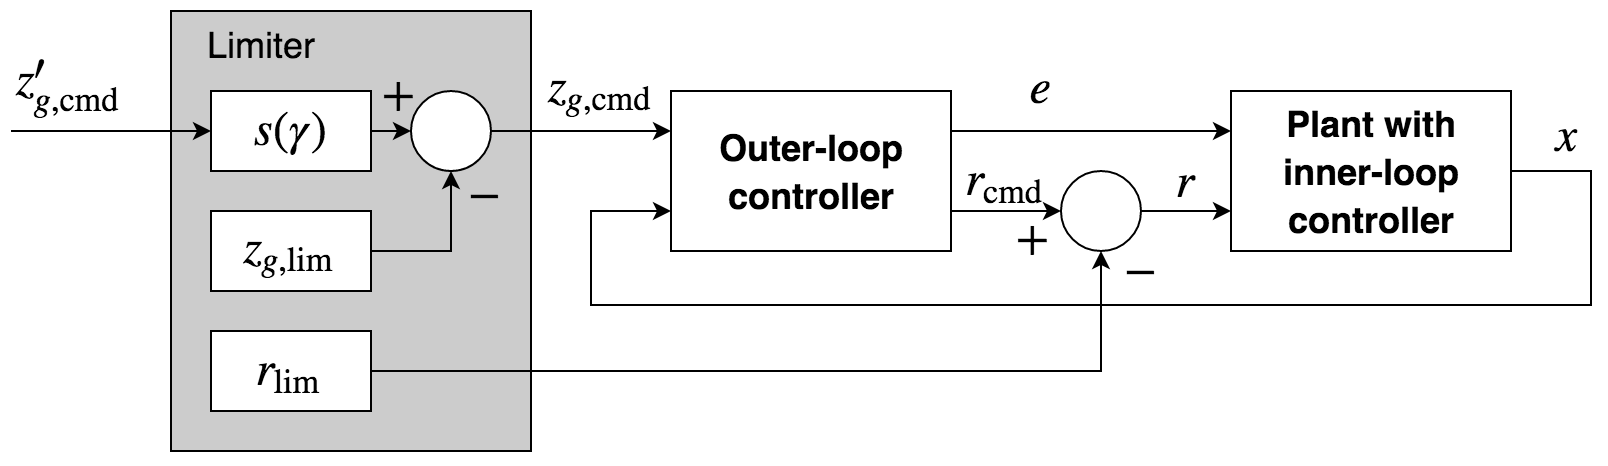
\includegraphics[width=5.5in]{\figurepath/simpleBlockWithLimiter.png}
    \vspace{-0.1in}
    \caption{Simplified outer-loop block diagram with limiter.\label{fig.simpleBlockWithLimiter}}
  \end{center}
\end{figure}

This modifies the block diagram in Figure~\ref{fig.innerAndOuterLoopDansOutputFeedback} as shown in Figure~\ref{fig.innerAndOuterLoopDansOutputFeedbackWithLimiter}.

\begin{figure}[H]
  \begin{center}
    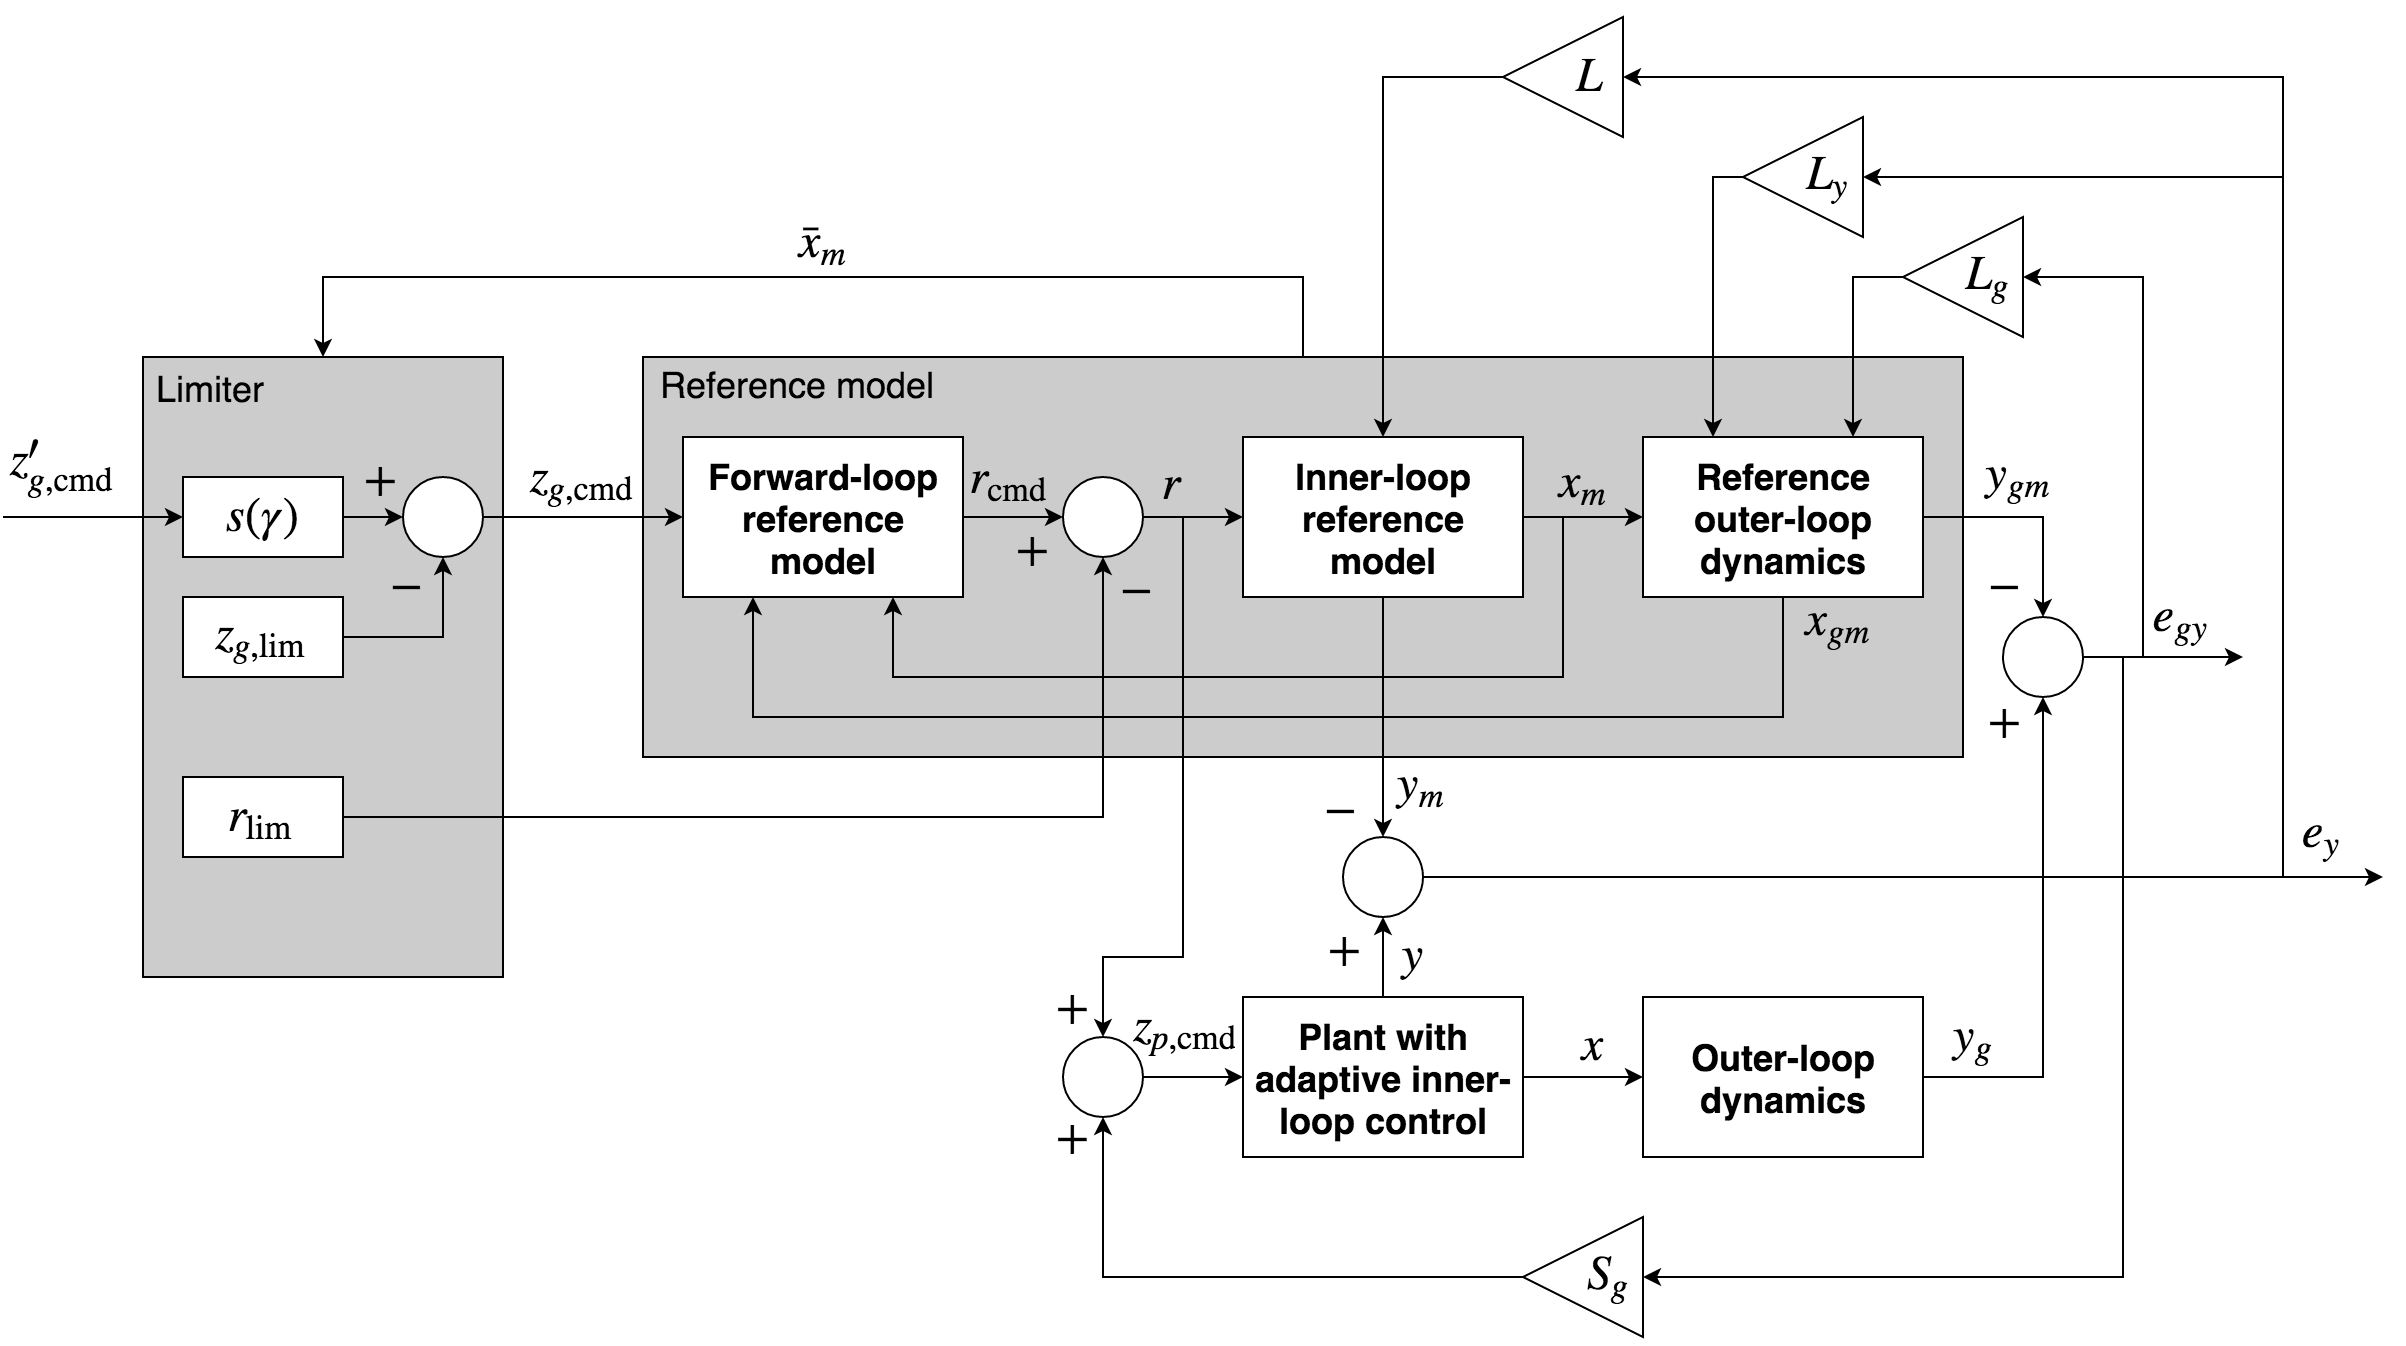
\includegraphics[width=6.5in]{\figurepath/innerAndOuterLoopDansOutputFeedbackWithLimiter.png}
    \vspace{-0.1in}
    \caption{Expanded outer-loop block diagram with limiter.\label{fig.innerAndOuterLoopDansOutputFeedbackWithLimiter}}
  \end{center}
\end{figure}

The entire reference model containing the inner-loop, the outer-loop, and forward-loop components is given in\ \eqref{eqn.xbareqnopenloop}.
When a controller as in\ \eqref{eqn.rKbar} is designed, with $\bar{K}$ as in\ \eqref{eqn.Kbar}, the entire reference model\ \eqref{eqn.xbareqnopenloop} is modified as
\begin{equation}
  \label{eqn.compactreferencemodel2}
  \begin{split}
    \dot{\bar{x}}_{m}(t)
    &=
    \bar{A}\bar{x}_{m}(t) + \bar{B}r(t) - \bar{L}_{y}e_{y}(t) - \bar{L}_{g}e_{gy}(t) + \bar{B}_{m}z_{g,\text{cmd}}^{\prime}(t) \\
    r_{\text{cmd}}(t)
    &=
    \bar{C}_{m}\bar{x}_{m}(t) \\
  \end{split}
\end{equation}
However, to facilitate command and state limiting the inner-loop command $r(t)$ and the outer-loop command $z_{g,\text{cmd}}(t)$ in\ \eqref{eqn.compactreferencemodel2} should be modified when certain reference model states become too large.
Thus inner-loop command $r(t)$ is no longer set as in\ \eqref{eqn.rrcmd} but instead as
\begin{equation}
  \label{eqn.rrcmdrlim}
  r(t) = r_{\text{cmd}}(t) - r_{\text{lim}}(t)
\end{equation}
where the inner-loop reference model command limiter $r_{\text{lim}}(t)$ is given by
\begin{equation}
  \label{eqn.rlim}
  r_{\text{lim}}(t) = -k_{r}\gamma K_{\text{lim}}\bar{x}_{m}(t)
\end{equation}
where $k_{r}\geq0$ has dimensions $k_{r}\in\mathbb{R}^{n_{ep}\times n_{ep}}$ and $K_{\text{lim}}\in\mathbb{R}^{n_{ep}\times n+n_{g}+n_{f}}$ is given by
\begin{equation}
  \label{eqn.Klim}
  K_{\text{lim}} = - R_{\text{lim}}(\bar{B}_{m}+\bar{B}k_{r})^{\top}\bar{P}
\end{equation}
where $R_{\text{lim}} = R_{\text{lim}}^{\top}\geq0$ has dimensions $R_{\text{lim}}\in\mathbb{R}^{n_{ep}\times n_{ep}}$ and $\bar{P}$ is the solution to the Lyapunov equation
\begin{equation}
  \label{eqn.LyapEqnPbar}
  \bar{A}_{m}^{\top}\bar{P}+\bar{P}\bar{A}_{m} = -\bar{Q}
\end{equation}
where $\bar{Q}=\bar{Q}^{\top}>0$.
The outer-loop command $z_{g,\text{cmd}}(t)$ is no longer selected as in\ \eqref{eqn.zgcmdzgcmdprime}, but is instead generated from the desired outer-loop command $z_{g,\text{cmd}}^{\prime}(t)$ as
\begin{equation}
  \label{eqn.zcmdlimited}
  z_{g,\text{cmd}}(t) = s\bigr(\gamma(\bar{x}_{m}(t))\bigr)z_{g,\text{cmd}}^{\prime}(t) - z_{g,\text{lim}}(t)
\end{equation}
where
\begin{equation}
  \label{eqn.sofgamma}
  s\bigr(\gamma(\bar{x}_{m}(t))\bigr) = 1-\gamma(\bar{x}_{m}(t))
\end{equation}
 and $z_{g,\text{lim}}(t)$ is given by
\begin{equation}
  \label{eqn.zglim}
  z_{g,\text{lim}}(t) = -\gamma K_{\text{lim}}\bar{x}_{m}(t)
\end{equation}
The scalar quantity $\gamma(\bar{x}_{m}(t))$ is the modulation function, which is a function of the entire reference model state $\bar{x}_{m}(t)$, and is selected such that $\gamma(\bar{x}_{m}(t))\in[0,1]$.
When $\gamma(\bar{x}_{m}(t))=0$ this corresponds to no state limiting, and when $\gamma(\bar{x}_{m}(t))=1$ this corresponds to the state limiter being fully active.
Thus, $\gamma(\bar{x}_{m}(t))$ is selected using several regions within the reference model state space such that within an inner region $\gamma(\bar{x}_{m}(t))=0$, an annulus region within which $\gamma(\bar{x}_{m}(t))$ varies between $0$ and $1$, and an outer region for which $\gamma(\bar{x}_{m}(t))=1$ as shown in Figure~\ref{fig.modulationFunction}.
See, for example the modulation function in Ref.\ \cite{lavretskywise.book.2013}.

\begin{figure}[H]
  \begin{center}
    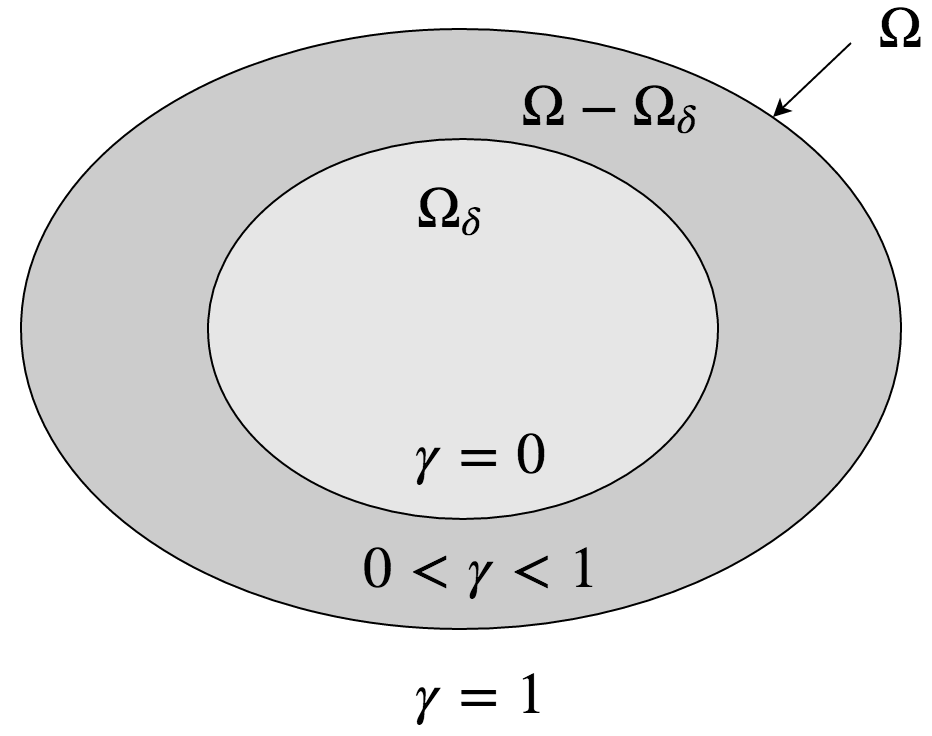
\includegraphics[width=2.5in]{\figurepath/limiterSets1.png}
    \vspace{-0.1in}
    \caption{State limiter modulation function regions from Ref.\cite{lavretsky.statelimiting.2010}\label{fig.modulationFunction}}
  \end{center}
\end{figure}

Using the outer-loop command $z_{g,\text{cmd}}(t)$ as generated by\ \eqref{eqn.zcmdlimited} into\ \eqref{eqn.compactreferencemodel2} gives
\begin{equation}
  \label{compactrefmodelwithlimiter}
  \begin{split}
    \dot{\bar{x}}_{m}(t)
    &=
    \bar{A}_{m}\bar{x}_{m}(t) + \bar{B}k_{r}\gamma(\bar{x}_{m}(t)) K_{\text{lim}}\bar{x}_{m} + \bar{B}_{m}\bigr(1-\gamma(\bar{x}_{m}(t))\bigr)z_{g,\text{cmd}}^{\prime}(t) \\
    & \qquad
    + \bar{B}_{m}\gamma(\bar{x}_{m}(t)) K_{\text{lim}}\bar{x}_{m}(t)-\bar{L}_{y}e_{y}(t) - \bar{L}_{g}e_{gy}(t) \\
    r_{\text{cmd}}(t)
    &=
    \bar{C}_{m}\bar{x}_{m}(t)
  \end{split}
\end{equation}
which can be further simplified as
\begin{equation}
  \label{compactrefmodelwithlimiter2}
  \begin{split}
    \dot{\bar{x}}_{m}(t)
    &=
    \bigr(\bar{A}_{m} + \bar{B}k_{r}\gamma(\bar{x}_{m}(t)) K_{\text{lim}} + \bar{B}_{m}\gamma(\bar{x}_{m}(t)) K_{\text{lim}}\bigr)\bar{x}_{m}(t) \\
    & \qquad
    + \bar{B}_{m}\bigr(1-\gamma(\bar{x}_{m}(t))\bigr)z_{g,\text{cmd}}^{\prime}(t) - \bar{L}_{y}e_{y}(t) - \bar{L}_{g}e_{gy}(t) \\
    r_{\text{cmd}}(t)
    &=
    \bar{C}_{m}\bar{x}_{m}(t)
  \end{split}
\end{equation}

\subsection{Stability}

Because the inner-loop reference model input $r(t)$ cancels out in the error dynamics in\ \eqref{eqn.errordynamics5}, and $z_{g,\text{cmd}}(t)$ is not present either, the state-limiter modification does not require any change to the Lyapunov function in\ \eqref{eqn.lyapfunction_2} to prove boundedness of the errors $e_{x}(t)$ and $e_{g}(t)$.
However, in the stability proof without the state limiter, the boundedness of $z_{g,\text{cmd}}(t)$, $e_{y}(t)$, and $e_{gy}(t)$ and stability of $\bar{A}_{m}$ in\ \eqref{eqn.compactreferencemodel} imply boundedness of the reference model states $x_{m}(t)$, $x_{gm}(t)$, and $x_{fm}(t)$, from which boundedness of the plant states $x(t)$ and $x_{g}(t)$ is concluded.
However, showing boundedness of the reference model states is less obvious when using the state limiter, which modifies the entire reference model dynamics in\ \eqref{eqn.compactreferencemodel} to obtain the limited reference model dynamics in\ \eqref{compactrefmodelwithlimiter}.
Thus it is necessary to ensure that with the limiting modifications the reference model state $\bar{x}_{m}(t)$ is still bounded, and global stability is still proved, as stated in the following theorem.

\begin{thm-dan}\label{thm.outerlooplimiter}
  The uncertain system in\ \eqref{eqn.wholeSystemUncertain} with inner-loop controller specified by the control law in\ \eqref{eqn.u}, update law in\ \eqref{eqn.updatelaw}, and the reference model in\ \eqref{eqn.refmodelWithBd} where $S_{1}$ and $L$ are chosen as described in Chapter~\ref{ch.innerLoop}, and the outer-loop controller specified by the outer-loop reference model in\ \eqref{eqn.refmodelouter}, forward-loop reference model component in\ \eqref{eqn.forwardloopcontroller}, with inner-loop command input $z_{p,\text{cmd}}(t)$ is prescribed by\ \eqref{eqn.zpcmd} and\ \eqref{eqn.egs}, where $r(t)$ is given by\ \eqref{compactrefmodelwithlimiter2},\ \eqref{eqn.rrcmdrlim}, and\ \eqref{eqn.rlim}, and outer-loop command generated by\ \eqref{eqn.zcmdlimited},\ \eqref{eqn.sofgamma}, and\ \eqref{eqn.zglim}, with $S_{g}$, $L_{g}$, and $L_{y}$ selected as described above, results in global stability, with $\lim_{t\rightarrow\infty}e_{x}(t)=0$ and $\lim_{t\rightarrow\infty}e_{g}(t)=0$.
\end{thm-dan}

\begin{proof-dan}
  This proof follows from the proof of Theorem~\ref{thm.outerloop} by proposing the same candidate Lyapunov function as in\ \eqref{eqn.lyapfunction_2} and differentiating to obtain\ \eqref{eqn.outerlooplyapderivative} from which it can be concluded that $e_{x}(t), \; e_{g}(t) , \;\widetilde{\Theta}(t)\in\mathcal{L}_{\infty}$.
  Bounds on $e_{x}(t)$ and $e_{g}(t)$ can be found as follows
  \begin{equation}
    \label{eqn.boundaonexandeg}
    \begin{split}
      \|e_{x}(t)\|
      & \leq
      \sqrt{\frac{V(0)}{\lambda_{\text{min}}(P_{x})}} \\
      \|e_{g}(t)\|
      & \leq
      \sqrt{\frac{V(0)}{\lambda_{\text{min}}(P_{g})}}
    \end{split}
  \end{equation}
  giving the following bounds on their respective measured output errors $e_{y}(t)$ and $e_{gy}(t)$ as
  \begin{equation}
    \label{eqn.boundaoneyandegy}
    \begin{split}
      \|e_{y}(t)\|
      & \leq
      e_{y,\text{max}}
      =
      \|C\|
      \sqrt{\frac{V(0)}{\lambda_{\text{min}}(P_{x})}} \\
      \|e_{gy}(t)\|
      & \leq
      e_{gy,\text{max}}
      =
      \|C_{g}\|
      \sqrt{\frac{V(0)}{\lambda_{\text{min}}(P_{g})}}
    \end{split}
  \end{equation}
  Propose the following additional candidate Lyapunov function to prove boundedness of the reference model state
  \begin{equation}
    \label{eqn.Lyapxmbar}
    \bar{V}\bigr(\bar{x}_{m}(t)\bigr) = \bar{x}_{m}^{\top}(t)\bar{P}\bar{x}_{m}(t)
  \end{equation}
  Differentiating\ \eqref{eqn.Lyapxmbar} gives
  \begin{equation}
    \label{eqn.Lyapxmbardot1}
    \dot{\bar{V}}\bigr(\bar{x}_{m}(t)\bigr)
    =
    \dot{\bar{x}}_{m}^{\top}(t)\bar{P}\bar{x}_{m}(t)
    + \bar{x}_{m}^{\top}(t)\bar{P}\dot{\bar{x}}_{m}(t)
  \end{equation}
  Substituting the limited reference model dynamics\ \eqref{compactrefmodelwithlimiter} into\ \eqref{eqn.Lyapxmbardot1} gives
  \begin{equation}
    \label{eqn.Lyapxmbardot2}
    \begin{split}
      \dot{\bar{V}}\bigr(\bar{x}_{m}(t)\bigr)
      &=
      \bigr(\bar{A}_{m}\bar{x}_{m}(t) + \bar{B}k_{r}\gamma(\bar{x}_{m}(t)) K_{\text{lim}}\bar{x}_{m}(t) + \bar{B}_{m}(1-\gamma(\bar{x}_{m}(t)))z_{g,\text{cmd}}^{\prime}(t) \\
      &\qquad
      +\bar{B}_{m}\gamma K_{\text{lim}}\bar{x}_{m}(t) - \bar{L}_{y}e_{y}(t) - \bar{L}_{g}e_{gy}(t)\bigr)^{\top}\bar{P}\bar{x}_{m}(t) \\
      &\qquad
      + \bar{x}_{m}^{\top}(t)\bar{P}\bigr(\bar{A}_{m}\bar{x}_{m}(t) + \bar{B}k_{r}\gamma(\bar{x}_{m}(t)) K_{\text{lim}}\bar{x}_{m}(t) + \bar{B}_{m}(1-\gamma(\bar{x}_{m}(t)))z_{g,\text{cmd}}^{\prime}(t) \\
      &\qquad
      + \bar{B}_{m}\gamma K_{\text{lim}}\bar{x}_{m}(t) - \bar{L}_{y}e_{y}(t) - \bar{L}_{g}e_{gy}(t)\bigr) \\
      &=
      \bar{x}_{m}^{\top}(t)\bigr(\bar{A}_{m}^{\top}\bar{P}+\bar{P}\bar{A}_{m}\bigr)\bar{x}_{m}(t)
      +\bar{x}_{m}^{\top}(t)K_{\text{lim}}^{\top}\gamma(\bar{x}_{m}(t)) k_{r}^{\top}\bar{B}^{\top}\bar{P}\bar{x}_{m}(t) \\
      &\qquad
      +\bar{x}_{m}^{\top}(t)\bar{P}\bar{B}k_{r}\gamma(\bar{x}_{m}(t)) K_{\text{lim}}\bar{x}_{m}(t)
      +\bar{x}_{m}^{\top}(t)K_{\text{lim}}^{\top}\gamma(\bar{x}_{m}(t))\bar{B}_{m}^{\top}\bar{P}\bar{x}_{m}(t) \\
      & \qquad
      +\bar{x}_{m}^{\top}(t)\bar{P}\bar{B}_{m}\gamma(\bar{x}_{m}(t)) K_{\text{lim}}\bar{x}_{m}(t)
      + 2\bar{x}_{m}^{\top}(t)\bar{P}\bar{B}_{m}(1-\gamma(\bar{x}_{m}(t)))z_{g,\text{cmd}}^{\prime}(t) \\
      & \qquad
      - 2\bar{x}_{m}^{\top}(t)\bar{P}(\bar{L}_{y}e_{y}(t) + \bar{L}_{g}e_{gy}(t)) \\
      &=
      \bar{x}_{m}^{\top}(t)\bigr(\bar{A}_{m}^{\top}\bar{P}+\bar{P}\bar{A}_{m}\bigr)\bar{x}_{m}(t)
      + \bar{x}_{m}^{\top}\bigr(K_{\text{lim}}^{\top}\gamma(\bar{x}_{m}(t)) k_{r}^{\top}\bar{B}^{\top}\bar{P}
      + \bar{P}\bar{B}k_{r}\gamma(\bar{x}_{m}(t)) K_{\text{lim}} \\
      &\qquad
      + K_{\text{lim}}^{\top}\gamma(\bar{x}_{m}(t))\bar{B}_{m}^{\top}\bar{P}
      +\bar{P}\bar{B}_{m}\gamma(\bar{x}_{m}(t)) K_{\text{lim}}\bigr) \bar{x}_{m}(t) \\
      & \qquad
      + 2\bar{x}_{m}^{\top}(t)\bar{P}\bar{B}_{m}\bigr(1-\gamma(\bar{x}_{m}(t))\bigr)z_{g,\text{cmd}}^{\prime}(t)
      - 2\bar{x}_{m}^{\top}(t)\bar{P}\bigr(\bar{L}_{y}e_{y}(t) + \bar{L}_{g}e_{gy}(t)\bigr) \\
      &=
      \bar{x}_{m}^{\top}(t)\bigr(\bar{A}_{m}^{\top}\bar{P}+\bar{P}\bar{A}_{m}\bigr)\bar{x}_{m}(t)
      +\bar{x}_{m}^{\top}(t)
      \bigr(K_{\text{lim}}^{\top}\gamma(\bar{x}_{m}(t)) (k_{r}^{\top}\bar{B}^{\top}+\bar{B}_{m}^{\top})\bar{P} \\
      &\qquad
      + \bar{P}(\bar{B}k_{r}+\bar{B}_{m})\gamma(\bar{x}_{m}(t)) K_{\text{lim}}\bigr) \bar{x}_{m}(t) \\
      & \qquad
      + 2\bar{x}_{m}^{\top}(t)\bar{P}\bar{B}_{m}\bigr(1-\gamma(\bar{x}_{m}(t))\bigr)z_{g,\text{cmd}}^{\prime}(t)
      - 2\bar{x}_{m}^{\top}(t)\bar{P}\bigr(\bar{L}_{y}e_{y}(t)+\bar{L}_{g}e_{gy}(t)\bigr) \\
    \end{split}
  \end{equation}
  Using $K_{\text{lim}}$ as in\ \eqref{eqn.Klim} where $\bar{P}$ is the solution to the Lyapunov equation\ \eqref{eqn.LyapEqnPbar}, the derivative in\ \eqref{eqn.Lyapxmbardot2} becomes
  \begin{equation}
    \label{eqn.Lyapxmbardot3}
    \begin{split}
      \dot{\bar{V}}\bigr(\bar{x}_{m}(t)\bigr)
      &=
      \bar{x}_{m}^{\top}(t)\bigr(\bar{A}_{m}^{\top}\bar{P}+\bar{P}\bar{A}_{m}\bigr)\bar{x}_{m}(t)
      -
      \bar{x}_{m}^{\top}(t)
      \bigr(
      \bar{P}(\bar{B}_{m}+\bar{B}k_{r})R_{\text{lim}}^{\top}\gamma(\bar{x}_{m}(t)) (k_{r}^{\top}\bar{B}^{\top}+\bar{B}_{m}^{\top})\bar{P} \\
      & \qquad
      +\bar{P}(\bar{B}k_{r}+\bar{B}_{m})R_{\text{lim}}(\bar{B}_{m}+\bar{B}k_{r})^{\top}\bar{P}
      \bigr) \bar{x}_{m}(t) \\
      & \qquad
      + 2\bar{x}_{m}^{\top}(t)\bar{P}\bar{B}_{m}\bigr(1-\gamma(\bar{x}_{m}(t))\bigr)z_{g,\text{cmd}}^{\prime}(t)
      - 2\bar{x}_{m}^{\top}(t)\bar{P}\bigr(\bar{L}_{y}e_{y}(t)+\bar{L}_{g}e_{gy}(t)\bigr) \\
      &=
      \bar{x}_{m}^{\top}(t)\bigr(\bar{A}_{m}^{\top}\bar{P}+\bar{P}\bar{A}_{m}\bigr)\bar{x}_{m}(t) \\
      &\qquad
      -\bar{x}_{m}^{\top}(t)
      \bigr(
      2\bar{P}(\bar{B}_{m}+\bar{B}k_{r})R_{\text{lim}}^{\top}\gamma(\bar{x}_{m}(t)) (k_{r}^{\top}\bar{B}^{\top}+\bar{B}_{m}^{\top})\bar{P}
      \bigr) \bar{x}_{m}(t) \\
      & \qquad
      + 2\bar{x}_{m}^{\top}(t)\bar{P}\bar{B}_{m}\bigr(1-\gamma(\bar{x}_{m}(t))\bigr)z_{g,\text{cmd}}^{\prime}(t)
      - 2\bar{x}_{m}^{\top}(t)\bar{P}\bigr(\bar{L}_{y}e_{y}(t)+\bar{L}_{g}e_{gy}(t)\bigr) \\
    \end{split}
  \end{equation}
  Using $\bar{Q}$ from\ \eqref{eqn.LyapEqnPbar} and defining the following
  \begin{equation}
    \label{eqn.qbarlim}
    \bar{Q}_{\rm{\lim}}(\gamma)
    =
    2\bar{P}(\bar{B}_{m}+\bar{B}k_{r})R_{\text{lim}}^{\top}\gamma (k_{r}^{\top}\bar{B}^{\top}+\bar{B}_{m}^{\top})\bar{P}
    \geq
    0
  \end{equation}
  allowing\ \eqref{eqn.Lyapxmbardot3} to be rewritten as
  \begin{equation}
    \label{eqn.vbardot}
    \begin{split}
      \dot{\bar{V}}\bigr(\bar{x}_{m}(t)\bigr)
      &=
      -\bar{x}_{m}^{\top}(t)(\bar{Q}+\bar{Q}_{\rm{\lim}}(\gamma))\bar{x}_{m}(t) + 2\bar{x}_{m}^{\top}(t)\bar{P}\bar{B}_{m}(1-\gamma)z_{g,\text{cmd}}^{\prime}(t) \\
      &\qquad
      - 2\bar{x}_{m}^{\top}(t)\bar{P}\bigr(\bar{L}_{y}e_{y}(t)+\bar{L}_{g}e_{gy}(t)\bigr) \\
      &=
      -\bar{x}_{m}^{\top}(\bar{Q}+\bar{Q}_{\rm{\lim}}(\gamma))\bar{x}_{m}(t) + 2\bar{x}_{m}^{\top}(t)\bar{P}\bigr(\bar{B}_{m}(1-\gamma)z_{g,\text{cmd}}^{\prime}(t) - \bar{L}_{y}e_{y}(t) - \bar{L}_{g}e_{gy}(t)\bigr)
    \end{split}
  \end{equation}
  Note that the bounds on $e_{y}(t)$ and $e_{gy}(t)$ in\ \eqref{eqn.boundaoneyandegy} are independent of $\bar{x}_{m}(t)$.
  Eq.\ \eqref{eqn.vbardot} contains a negative quadratic term in $\bar{x}_{m}(t)$, and a sign indefinite term which is linear in $\bar{x}_{m}(t)$.
  Thus, for sufficiently large $\bar{x}_{m}(t)$, the derivative $\dot{\bar{V}}\bigr(x_{m}(t)\bigr)$ in\ \eqref{eqn.vbardot} becomes strictly negative.
  This is quantified precisely by the following statement: $\dot{\bar{V}}\bigr(\bar{x}_{m}(t)\bigr)<0$ outside the compact set
  \begin{equation}
    \label{eqn.limiterCompactSet}
    E_{\delta}=
    \biggr\{
    \bar{x}_{m}(t)\in\mathbb{R}^{n} \; : \;
    \|\bar{x}_{m}(t)\|
    \leq
    \frac{2\lambda_{\text{max}}(\bar{P})\bigr(
    \|\bar{B}_{m}\|(1-\gamma)z_{g,\text{cmd,max}}^{\prime}+
    \|\bar{L}_{y}\|e_{y,\text{max}}+\|\bar{L}_{g}\|e_{gy,\text{max}}
    \bigr)}{\lambda_{\text{min}}(\bar{Q}+\bar{Q}_{\text{lim}}(\gamma))}
    \biggr\}
  \end{equation}
  for all $\gamma(\bar{x}_{m}(t))\in[0,1]$.
  Thus the entire reference model state $\bar{x}_{m}(t)$ is bounded\ \cite{narendra.stable.2005} which, with the boundedness of the errors $e_{x}(t)$ and $e_{g}(t)$, implies that $x(t),\;x_{g}(t)\in\mathcal{L}_{\infty}$.
  With $e_{x}(t),\;e_{g}(t),\;x_{m}(t),\;\widetilde{\Theta}\in\mathcal{L}_{\infty}$, and the the error dynamics in\ \eqref{eqn.innerAndOuterLoopErrorDynamics2}, this implies that $\dot{e}_{x}(t), \; \dot{e}_{g}(t)\in\mathcal{L}_{\infty}$.
  Finally, $\int_{0}^{t}\dot{V}(\tau)d\tau=V(t)-V(0)$ and since $V(t)$ is non-increasing and positive definite, $V(0)-V(t)\leq V(0)$.
  This gives $-\int_{0}^{t}\dot{V}(\tau)d\tau\leq V(0)$.
  Substituting in the expression for $\dot{V}= - e_{x}^{\top}(t)Q_{x}e_{x}(t) - e_{g}^{\top}(t)Q_{g}e_{g}(t)$ gives $\int_{0}^{t}e_{x}(\tau)^{\top}Q_{x}e_{x}(\tau) + e_{g}(\tau)^{\top}Q_{g}e_{g}(\tau)d\tau\leq V(0)$ and in turn that $e_{x}(t),\;e_{g}(t)\in\mathcal{L}_{2}$.
  With this, it can be concluded using Barbalat's Lemma\ \cite{narendra.stable.2005} that $\lim_{t\rightarrow\infty}e_{x}(t)=0$ and $\lim_{t\rightarrow\infty}e_{g}(t)=0$.
\end{proof-dan}

Theorem~\ref{thm.outerlooplimiter} proves stability of the closed-loop system with state limiter, with asymptotic tracking of the reference model states $x_{m}(t)$ and $x_{gm}(t)$ by the plant states $x(t)$ and $x_{g}(t)$, respectively.
In the absence of the state limiter, satisfaction of the control goal of outer-loop command tracking was discussed in Corollary~\ref{cor.zgcmdtracking}.
When using the state limiter, Theorem~\ref{thm.outerloop}, like Theorem~\ref{thm.outerlooplimiter}, provided $z_{g}(t)\rightarrow z_{gm}(t)$ as $t\rightarrow\infty$.
However, without the limiter, the reference model in\ \eqref{eqn.compactreferencemodel} was selected so that $z_{gm}(t)$ was a filtered version of the outer-loop command, so that asymptotic tracking of constant commands was achieved, as given by Corollary~\ref{cor.zgcmdtracking}.
When using the limiter, the reference model dynamics in\ \eqref{compactrefmodelwithlimiter} are modified such that $z_{gm}(t)$ is no longer simply a filtered version of the outer-loop command $z_{g,\text{cmd}}^{\prime}(t)$.
Thus asymptotic tracking of $z_{g,\text{cmd}}^{\prime}(t)$ by $z_{g}(t)$ doesn't hold in general, due to the scaling of the outer-loop command by the limiter.
However, if a desired outer-loop command $z_{g,\text{cmd}}^{\prime}(t)$ is given such that the limiter is inactive and $\gamma\bigr(\bar{x}_{m}(t)\bigr)=0$, the same conclusion as in Corollary~\ref{cor.zgcmdtracking} can be made, with $z_{g,\text{cmd}}(t) = z_{g,\text{cmd}}^{\prime}(t)$.
This statement is formalized in the following corollary to Theorem~\ref{thm.outerlooplimiter}.

\begin{cor-dan}\label{cor.notForcingLimiting}
  For all piecewise constant outer-loop command inputs $z_{g,\text{\rm{cmd}}}^{\prime}(t)$ which satisfy $\|z_{g,\text{\rm{cmd}}}^{\prime}(t)\|_{\infty}\leq z_{g,\text{\rm{cmd,max}}}^{\prime}$, the outer-loop regulated output $z_{g}(t)$ tracks $z_{g,\text{\rm{cmd}}}^{\prime}(t)$ asymptotically, where $z_{g,\text{\rm{cmd,max}}}^{\prime}$ is given by
  \begin{equation}
    \label{eqn.zgcmdprimemax}
    z_{g,\text{\rm{cmd,max}}}^{\prime}=
    \frac{\bar{x}_{m,\text{\rm{max}}}}{\|h_{m}\|_{1}}
  \end{equation}
  where $h_{m}$ is the impulse response of the nominal reference model, given by\ \eqref{compactrefmodelwithlimiter2} with $\gamma(\bar{x}_{m}(t))=0$, $\bar{L}_{y}=0$ and $\bar{L}_{g}=0$, and $\bar{x}_{m,\text{\rm{max}}}=\text{\rm{max}}_{\bar{x}_{m}(t)\in\Omega_{\delta}}\|\bar{x}_{m}(t)\|$.
\end{cor-dan}

\begin{proof-dan}
  For all $\bar{x}_{m}(t)\in\Omega_{\delta}$ the state limiter is inactive, and the evolution of the reference model state $\bar{x}_{m}(t)$ is governed by\ \eqref{compactrefmodelwithlimiter2} with $\gamma(\bar{x}_{m}(t))=0$, while $e_{y}(t)$ and $e_{gy}(t)$ tend to zero asymptotically.
  Thus, the reference model state $\bar{x}_{m}(t)$ ultimately depends only on the command input $z_{g,\text{cmd}}^{\prime}(t)$.
  The following bound on the reference model state holds, where $h_{m}$ is the impulse response of the nominal reference model,\ \eqref{compactrefmodelwithlimiter2} with $\gamma(\bar{x}_{m}(t))=0$.
  \begin{equation*}
    \|\bar{x}_{m}(t)\|_{\infty}=\bar{x}_{m,\text{max}} \leq \|h_{m}\|_{1}\|z_{g,\text{cmd}}^{\prime}(t)\|_{\infty}
  \end{equation*}
  From this, the bound on the command input can be found as in\ \eqref{eqn.zgcmdprimemax} that ensures the reference model state $\bar{x}_{m}(t)\in\Omega_{\delta}$, thus not invoking the state limiter, and providing the tracking properties given in Corollary~\ref{cor.zgcmdtracking}.
\end{proof-dan}

\begin{rem-dan}
  Corollary~\ref{cor.notForcingLimiting} states that if the desired outer-loop command $z_{g,\text{cmd}}^{\prime}(t)$ is such that the system is not driven to enter the limiting region, that the limiter will not impact tracking performance of the system.
  This is due to the fact that the convergence of the tracking errors $e_{y}(t)$ and $e_{gy}(t)$ to zero is obtained regardless of whether the limiter is invoked or not.
  In other words, as these errors tend to zero, only the desired outer-loop command $z_{g,\text{cmd}}^{\prime}(t)$ can drive the reference model state $\bar{x}_{m}(t)$ out of $\Omega_{\delta}$, as governed by\ \eqref{eqn.compactreferencemodel}.
  Thus, if the desired outer-loop command is such that it does not force $\bar{x}_{m}(t)$ outside of $\Omega_{\delta}$, the limiter will become inactive.
  Corollary~\ref{cor.notForcingLimiting} then finds the maximum value of $z_{g,\text{cmd}}^{\prime}(t)$ such that $\bar{x}_{m}(t)\in\Omega_{\delta}$ using the impulse response of the reference model.
\end{rem-dan}

\begin{rem-dan}
  The benefits of the state limiter are apparent from the compact set in\ \eqref{eqn.limiterCompactSet} outside of which $\dot{\bar{V}}(\bar{x}_{m}(t))<0$.
  The size of $E_{\delta}$ monotonically decreases in size as $\gamma(\bar{x}_{m}(t))$ increases, hence shrinking the bound on $\bar{x}_{m}(t)$ when the limiter is invoked, versus without the limiter.
\end{rem-dan}

\subsubsection{Degrees of Freedom}

The limiter described above has several degrees of freedom which can be chosen by the designer to achieve the desired performance.
These degrees of freedom are the gains $k_{r}$, $R_{\text{lim}}$, $\bar{Q}$, and the modulation function $\gamma(\bar{x}_{m}(t))$ and the corresponding sets $\Omega$ and $\Omega_{\delta}$.
The limiter components $r_{\text{lim}}(t)$ and $z_{g,\text{lim}}(t)$ enter through the input matrices $\bar{B}$ and $\bar{B}_{m}$, respectively, of the reference model in\ \eqref{eqn.compactreferencemodel2}.
The matrix $R_{\text{lim}}$ scales $K_{\text{lim}}$ in\ \eqref{eqn.Klim}, which is the gain used in both of the limiting components $r_{\text{lim}}(t)$ and $z_{g,\text{lim}}(t)$, whereas $k_{r}$ scales only $r_{\text{lim}}(t)$.
Thus, by adjusting $R_{\text{lim}}$ and $k_{r}$, the relative influence of the limiter through $\bar{B}$ and $\bar{B}_{m}$ can be changed.
This alters the the effective reference model matrix in\ \eqref{compactrefmodelwithlimiter2} when the limiter becomes active, and thus $\bar{Q}_{\rm{\lim}}(\gamma(\bar{x}_{m}(t)))$ in\ \eqref{eqn.qbarlim}.
This, along with the matrix $\bar{Q}$, alters the region outside of which $\dot{\bar{V}}<0$, and thus affects the time response of the system when the state limiter is active.
With $k_{r}=0$ and $R_{\text{lim}}=0$ the limiter would still be stable, however the only adjustment would come through the reduction of the outer-loop command $z_{g,\text{cmd}}^{\prime}(t)$ in\ \eqref{eqn.vbardot}.
The modulation function $\gamma(\bar{x}_{m}(t))$ simply defines based on $\bar{x}_{m}$ when the limiter becomes active, and can be selected so as to depend on the various elements of $\bar{x}_{m}(t)$ as desired.

\subsection{Complete Controller Summary with Limiter}

The entire system closed-loop system, consisting of the plant and controller, can be summarized with the following set of equations.
The uncertain plant\ \eqref{eqn.uncsystemWithBd}, the outer-loop dynamics\ \eqref{eqn.outerLoopDynamics}, the inner-loop reference model\ \eqref{eqn.refmodelWithBd}, outer-loop reference model\ \eqref{eqn.refmodelouter}, forward-loop reference model component\eqref{eqn.forwardloopcontroller}, with inner-loop command input prescribed by\ \eqref{eqn.rrcmdrlim},\ \eqref{eqn.zpcmd} and\ \eqref{eqn.egs},\ \eqref{eqn.rlim} and outer-loop command generated by\ \eqref{eqn.zcmdlimited},\ \eqref{eqn.sofgamma}, and\ \eqref{eqn.zglim}, control law\eqref{eqn.u}, inner-loop command input\ \eqref{eqn.zpcmd} and\ \eqref{eqn.egs}, and update law\ \eqref{eqn.updatelaw} together are summarized as follows.

\begin{equation*}
  \begin{aligned}
    \textbf{Plant:}
    && \dot{x}(t) &= Ax(t) + B\bigr(\Lambda u(t) + \Psi^{\top}x(t)\bigr) + B_{\text{cmd}}z_{p,\text{cmd}}(t) + B_{d}x_{g}(t) \\
    && \dot{x}_{g}(t) &= A_{g}x_{g}(t) + B_{g}x(t) \\
    \textbf{Reference model:}
    && \dot{x}_{m}(t) &= A_{m}x_{m}(t) + B_{\text{cmd}}r(t) - Le_{y}(t) + B_{d}x_{gm}(t) \\
    && \dot{x}_{gm}(t) &= B_{g}x_{m}(t) + A_{g}x_{gm}(t) - L_{y}e_{y}(t) - L_{g}e_{gy}(t) \\
    && \dot{x}_{fm}(t) &= B_{f3}x_{m}(t) + B_{f2}x_{gm}(t) + A_{fm}x_{fm}(t) + B_{f1}z_{g,\text{cmd}}(t) \\
    \textbf{Command:}
    && r_{\text{cmd}}(t) &= C_{fm}x_{fm}(t) + D_{f1}z_{g,\text{cmd}}(t) + D_{f2}x_{gm}(t) + D_{f3} x_{m}(t) \\
    && r(t) &= r_{\text{cmd}}(t) - r_{\text{lim}}(t) \\
    && r_{\text{lim}}(t) &= -k_{r}\gamma\bigr(\bar{x}_{m}(t)\bigr) K_{\text{lim}}\bar{x}_{m}(t) \\
    && z_{g,\text{cmd}}(t) &= s(\gamma)z_{g,\text{cmd}}^{\prime}(t) - z_{g,\text{lim}}(t) \\
    && z_{p,\text{cmd}}(t) &= r(t) + S_{g}e_{gy}(t) \\
    \textbf{Errors:}
    && e_{y}(t) &= C\bigr(x(t)-x_{m}(t)\bigr) \\
    && e_{gy}(t) &= C_{g}\bigr(x_{g}(t) - x_{gm}(t)\bigr) \\
    \textbf{Control:}
    && u(t) &= \bigr(K_{x}+\Theta(t)\bigr)^{\top}x_{m}(t) \\
    && \dot{\Theta}(t) &= -\Gamma x_{m}(t)\bigr(S_{1}e_{y}(t)\bigr)^{\top}\text{sgn}(\Lambda) \\
  \end{aligned}
\end{equation*}

\section{Numerical Examples}\label{sec.outerLoopNumericalExample}

\subsection{Example 1: Inverted Pendulum Cart}

The inverted pendulum on a cart example from Section~\ref{sec.innerLoopNumericalExample} is continued here.
In the first part of this example, the inner-loop adaptive controller was used to accommodate uncertainties in the viscous damping coefficients and force input, and enforced tracking of the commanded cart velocity.
The example is continued here using the plant with this adaptive inner-loop, and the outer-loop controller prescribe the necessary cart velocity command so as to track pendulum position commands.
The pendulum position was selected as the output so as to satisfy the rank condition in\ \eqref{eqn.gsvdmatrixfullrank}, requiring that the outer-loop output supply sufficient information about the system beyond simply an integration of the inner-loop output.
This is essentially the statement that if the entire system as in the form\ \eqref{eqn.wholeSystemUncertain} is not observable through only $y_{p}(t)$, that integrating this output will not make it observable.

\begin{figure}[H]
  \begin{center}
    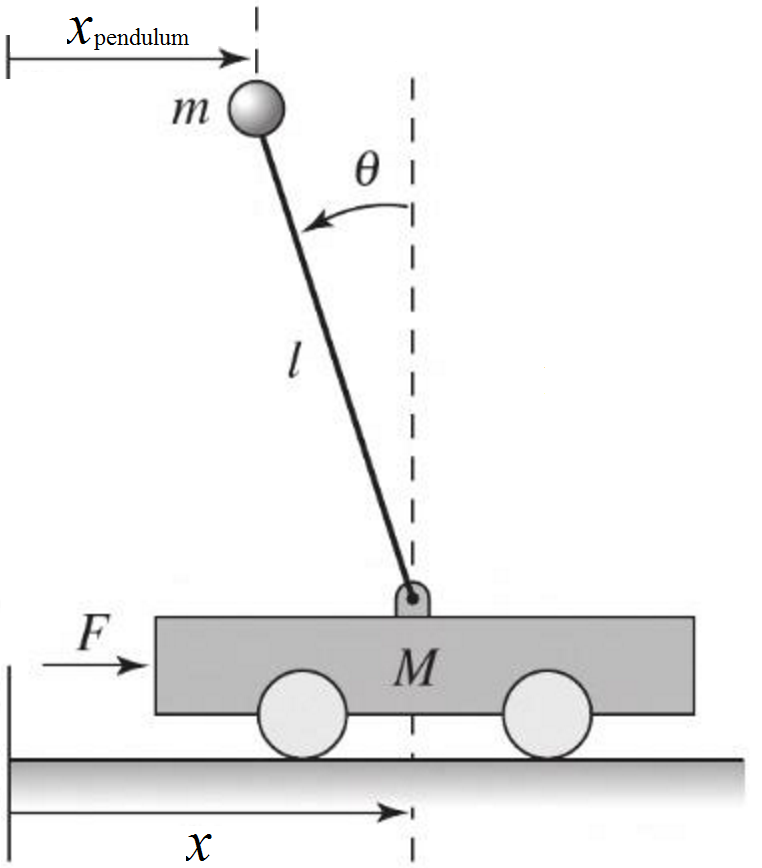
\includegraphics[width=2.8in]{\figurepath/pendulumCart.png}
    \vspace{-0.1in}
    \caption{Inverted pendulum on cart from Ref.\ \cite{astrom.feedbackintro.2010}.\label{fig.pendulumCart}}
  \end{center}
\end{figure}

The pendulum cart dynamics in\ \eqref{eqn.pendulumCartWhole} were partitioned into the inner-loop dynamics in\ \eqref{eqn.pendulumCartInnerLoop} and the outer-loop dynamics in the form of\ \eqref{eqn.outerLoopDynamics} given in\ \eqref{eqn.pendulumCartOuterLoop} below
\begin{equation}
  \label{eqn.pendulumCartOuterLoop}
  \begin{split}
    \begin{bmatrix}
      \dot{\theta} \\
      \dot{x}
    \end{bmatrix}
    &=
    \begin{bmatrix}
      0 & 0 \\
      0 & 0 \\
    \end{bmatrix}
    \begin{bmatrix}
      \theta \\
      x
    \end{bmatrix}
    +
    \begin{bmatrix}
      1 & 0 \\
      0 & 1 \\
    \end{bmatrix}
    \begin{bmatrix}
      \dot{\theta} \\
      \dot{x} \\
    \end{bmatrix} \\
    x_{\text{pendulum}}
    &=
    \begin{bmatrix}
      l & 1
    \end{bmatrix}
    \begin{bmatrix}
      \theta \\
      x
    \end{bmatrix}
  \end{split}
\end{equation}
The matrix $B_{gd}$ which couples outer-loop kinematics into the inner-loop dynamics is given by the following
\begin{equation*}
  B_{gd}
  =
  \begin{bmatrix}
    \frac{M_{t}mgl}{\mu} & 0 \\
    \frac{m^{2}g^{2}l}{\mu} & 0
  \end{bmatrix}
\end{equation*}
Using the numerical values for the pendulum given in Section\ref{sec.innerLoopNumericalExample}, the relevant matrices are given by
\begin{equation*}
  A_{g} =
  \begin{bmatrix}
    0 & 0 \\
    0 & 0
  \end{bmatrix}
  \qquad
  B_{gp} =
  \begin{bmatrix}
    1 & 0 \\
    0 & 1
  \end{bmatrix}
  \qquad
  C_{g} =
  \begin{bmatrix}
    1 \\
    1
  \end{bmatrix}^{\top}
  \qquad
  C_{gz} =
  \begin{bmatrix}
    1 \\
    1
  \end{bmatrix}^{\top}
  \qquad
  B_{gd} =
  \begin{bmatrix}
    19.6 & 0 \\
    96.04 & 0
  \end{bmatrix}^{\top}
\end{equation*}
The forward-loop reference model was designed using integral action on the regulated output as in\ \eqref{eqn.rKbar} using the following weighting matrices
\begin{equation*}
  \begin{split}
    Q_{\text{lqr}}
    &=
    \text{diag}\bigr(
    \begin{bmatrix}
      0 & 0 & 0 & 0 & 0 & 1
    \end{bmatrix}
    \bigr) \\
    R_{\text{lqr}}
    &=
    0.01
  \end{split}
\end{equation*}
Using the outer-loop design procedure summarized in Section~\ref{sec.outerLoopDesignProcedureSummary}, $P_{g}$ was calculated as in\ \eqref{eqn.Pg} using $P$ calculated as in\ \eqref{eqn.P} and $X_{D}$, where $P_{\Lambda}$ in\ \eqref{eqn.P}, and $X_{D}$ was selected as
\begin{equation*}
  X_{D}
  =
  \begin{bmatrix}
    1.0001 & 0.0086621 \\
    0.0086621 & 1
  \end{bmatrix}
  \qquad
  P_{\Lambda}
  =
  \begin{bmatrix}
    0.025 & 0 \\
    0 & 0.025
  \end{bmatrix}
\end{equation*}
With the resulting $P_{g}$, $S_{g}$ was determined using\ \eqref{eqn.SgCaseI}, and $L_{g}$ obtained numerically satisfying\ \eqref{eqn.condition4a}.
Finally $L_{y}$ was computed using\ \eqref{eqn.Ly} thus completing the outer-loop control design.

The following plot in Fig.~\ref{fig.outerLoopPendulumCart} shows the response of the closed-loop system to track pendulum position commands, when subject to the same uncertainties described in Section\ref{sec.innerLoopNumericalExample}.
As in the first example, the plot shows the baseline controller applied to the nominal plant until $t=10$ seconds when the uncertainty is introduced.
At $t=30$ seconds the adaptive controller is turned on.
As in the inner-loop example, the adaptive element ensures stability in the presence of the uncertainty, and outer-loop command tracking is provided.
However, there are significant oscillations in the response due to the uncertainty, with the pendulum reaching angular velocities of 200 deg/s.
Fig.~\ref{fig.outerLoopStateLimiterPendulumCart} shows the response of the same system, but with the limiter used to limit the angular velocity of the pendulum to within 80 deg/s.

\newpage
\begin{figure}[H]
  \hspace{-0.25in}
  \noindent\makebox[7.0in]{%
  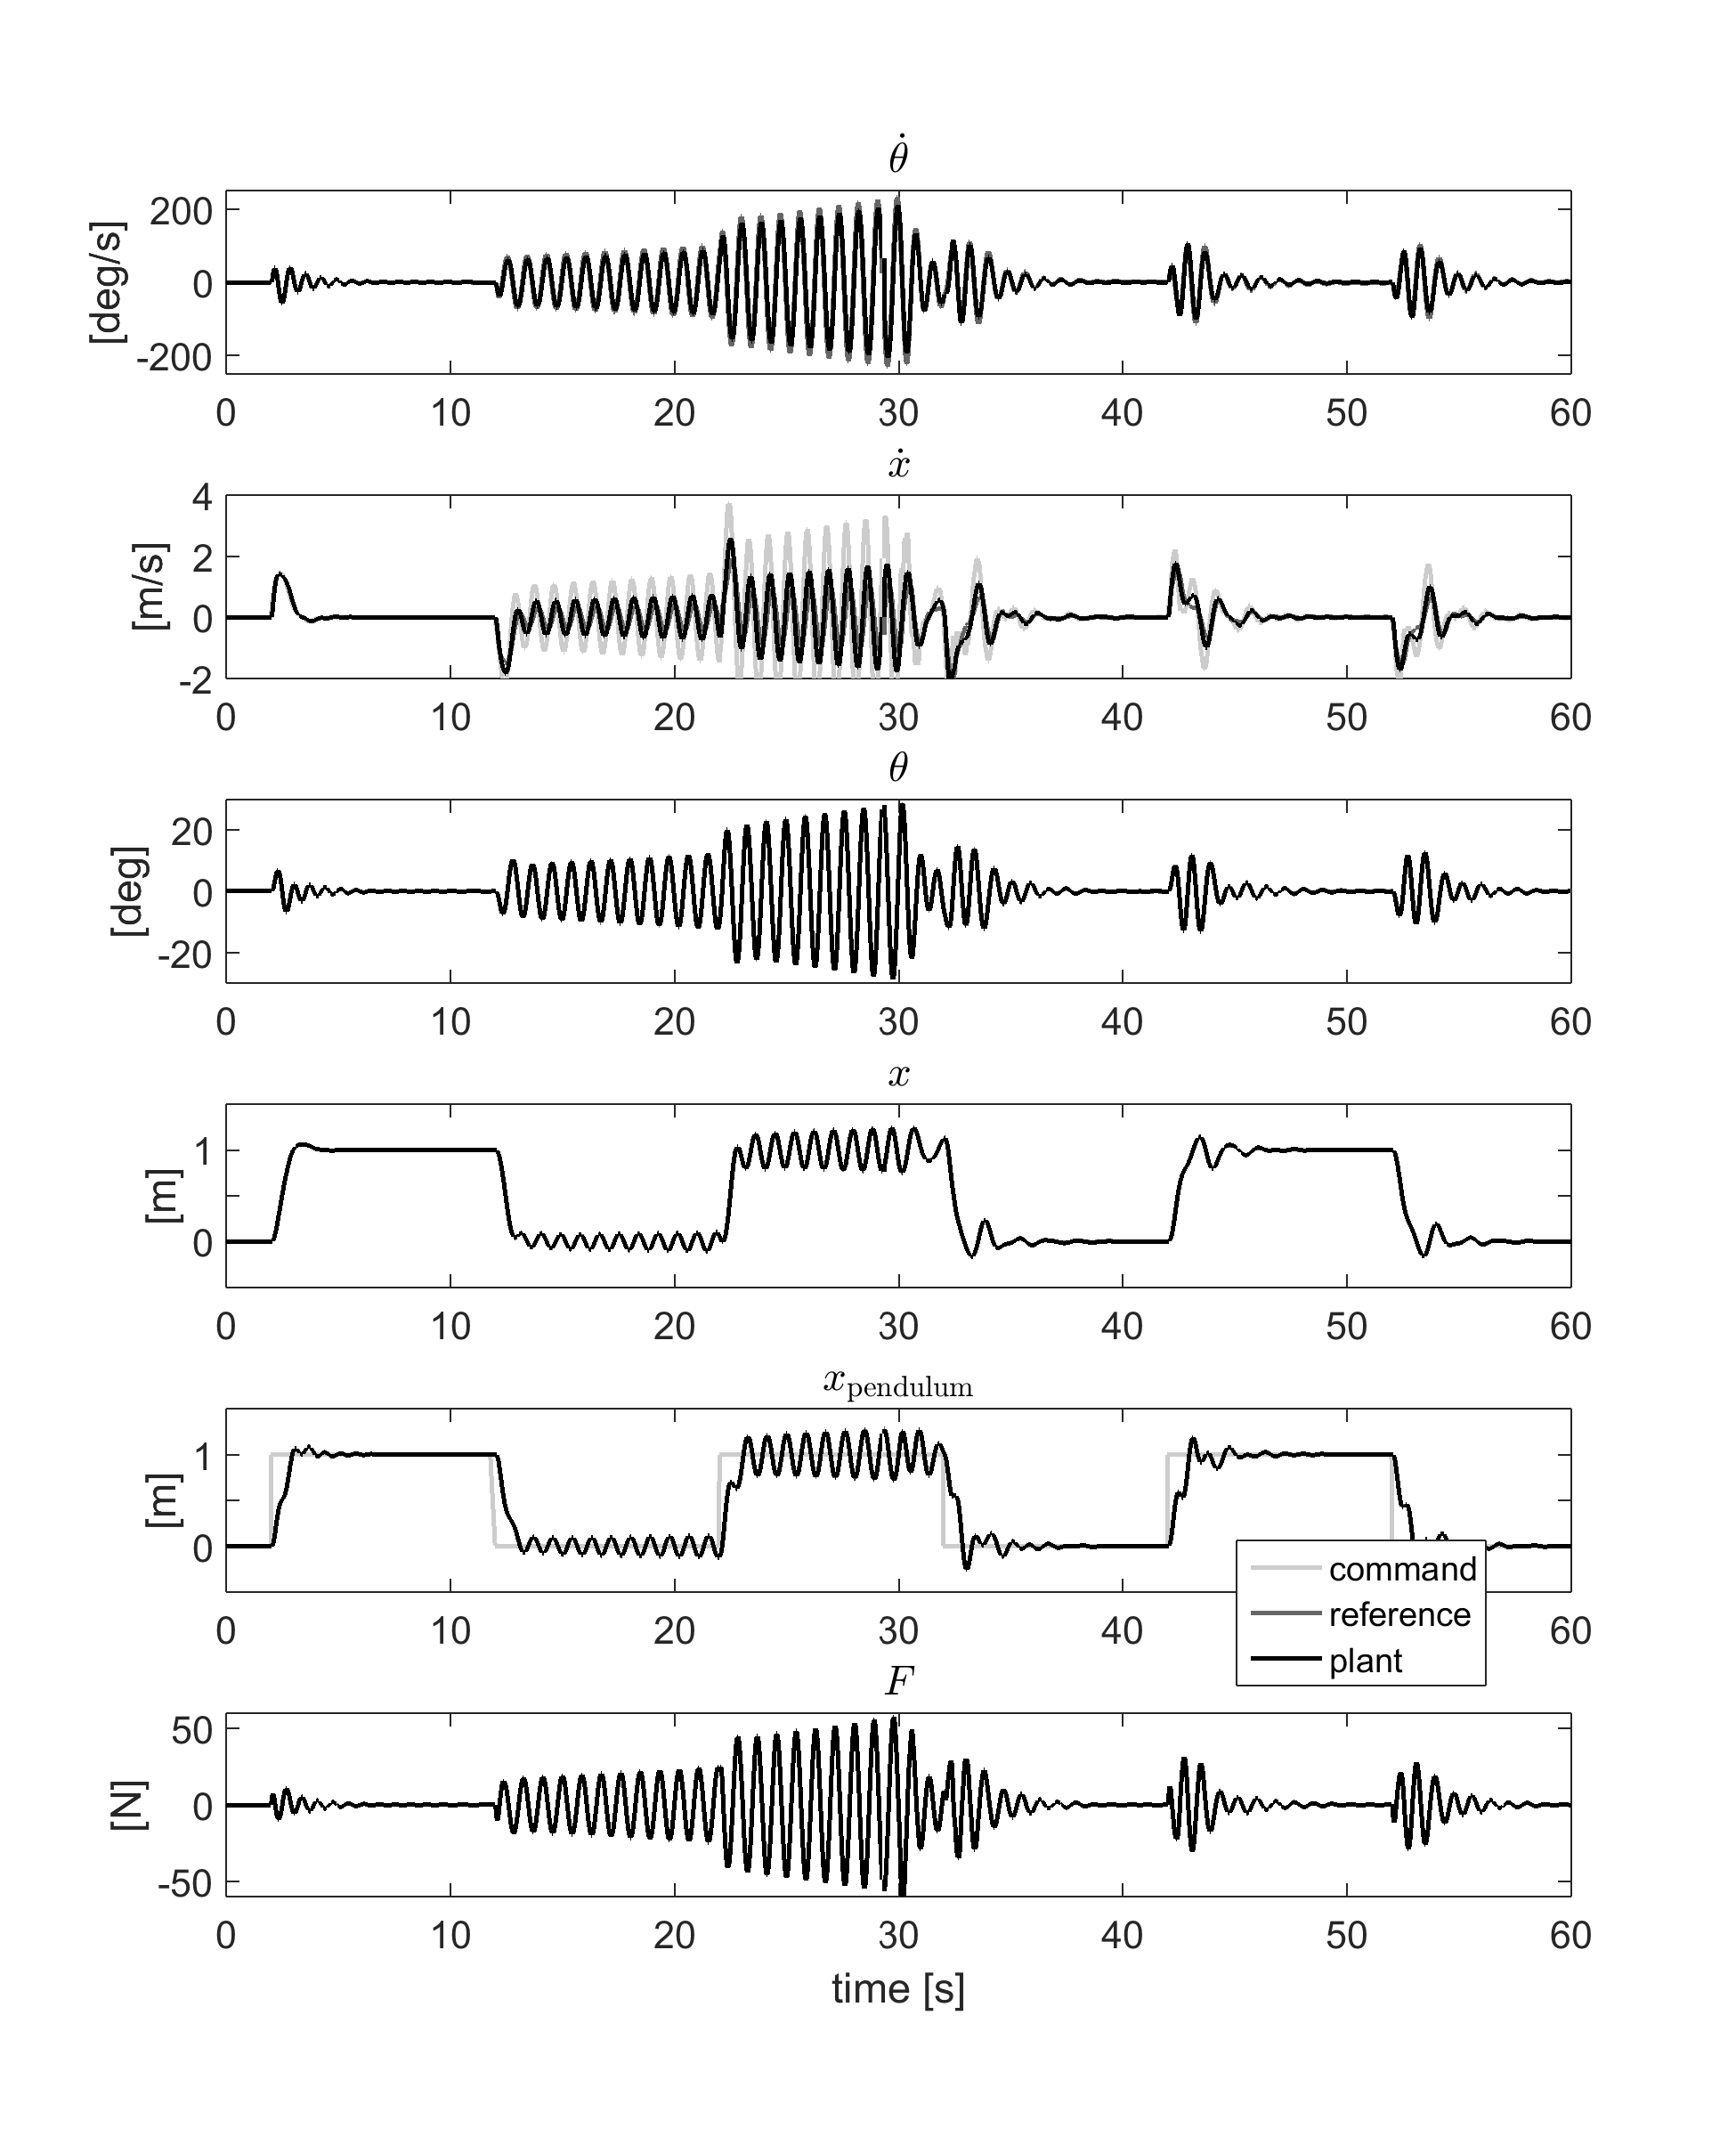
\includegraphics[width=7.0in]{\figurepath/outerLoopPendulumCart.png}}
  \vspace{-0.95in}
  \caption{Time response of pendulum cart with inner and outer-loop controller.\label{fig.outerLoopPendulumCart}}
\end{figure}

\newpage
\begin{figure}[H]
  \hspace{-0.25in}
  \noindent\makebox[7.0in]{%
  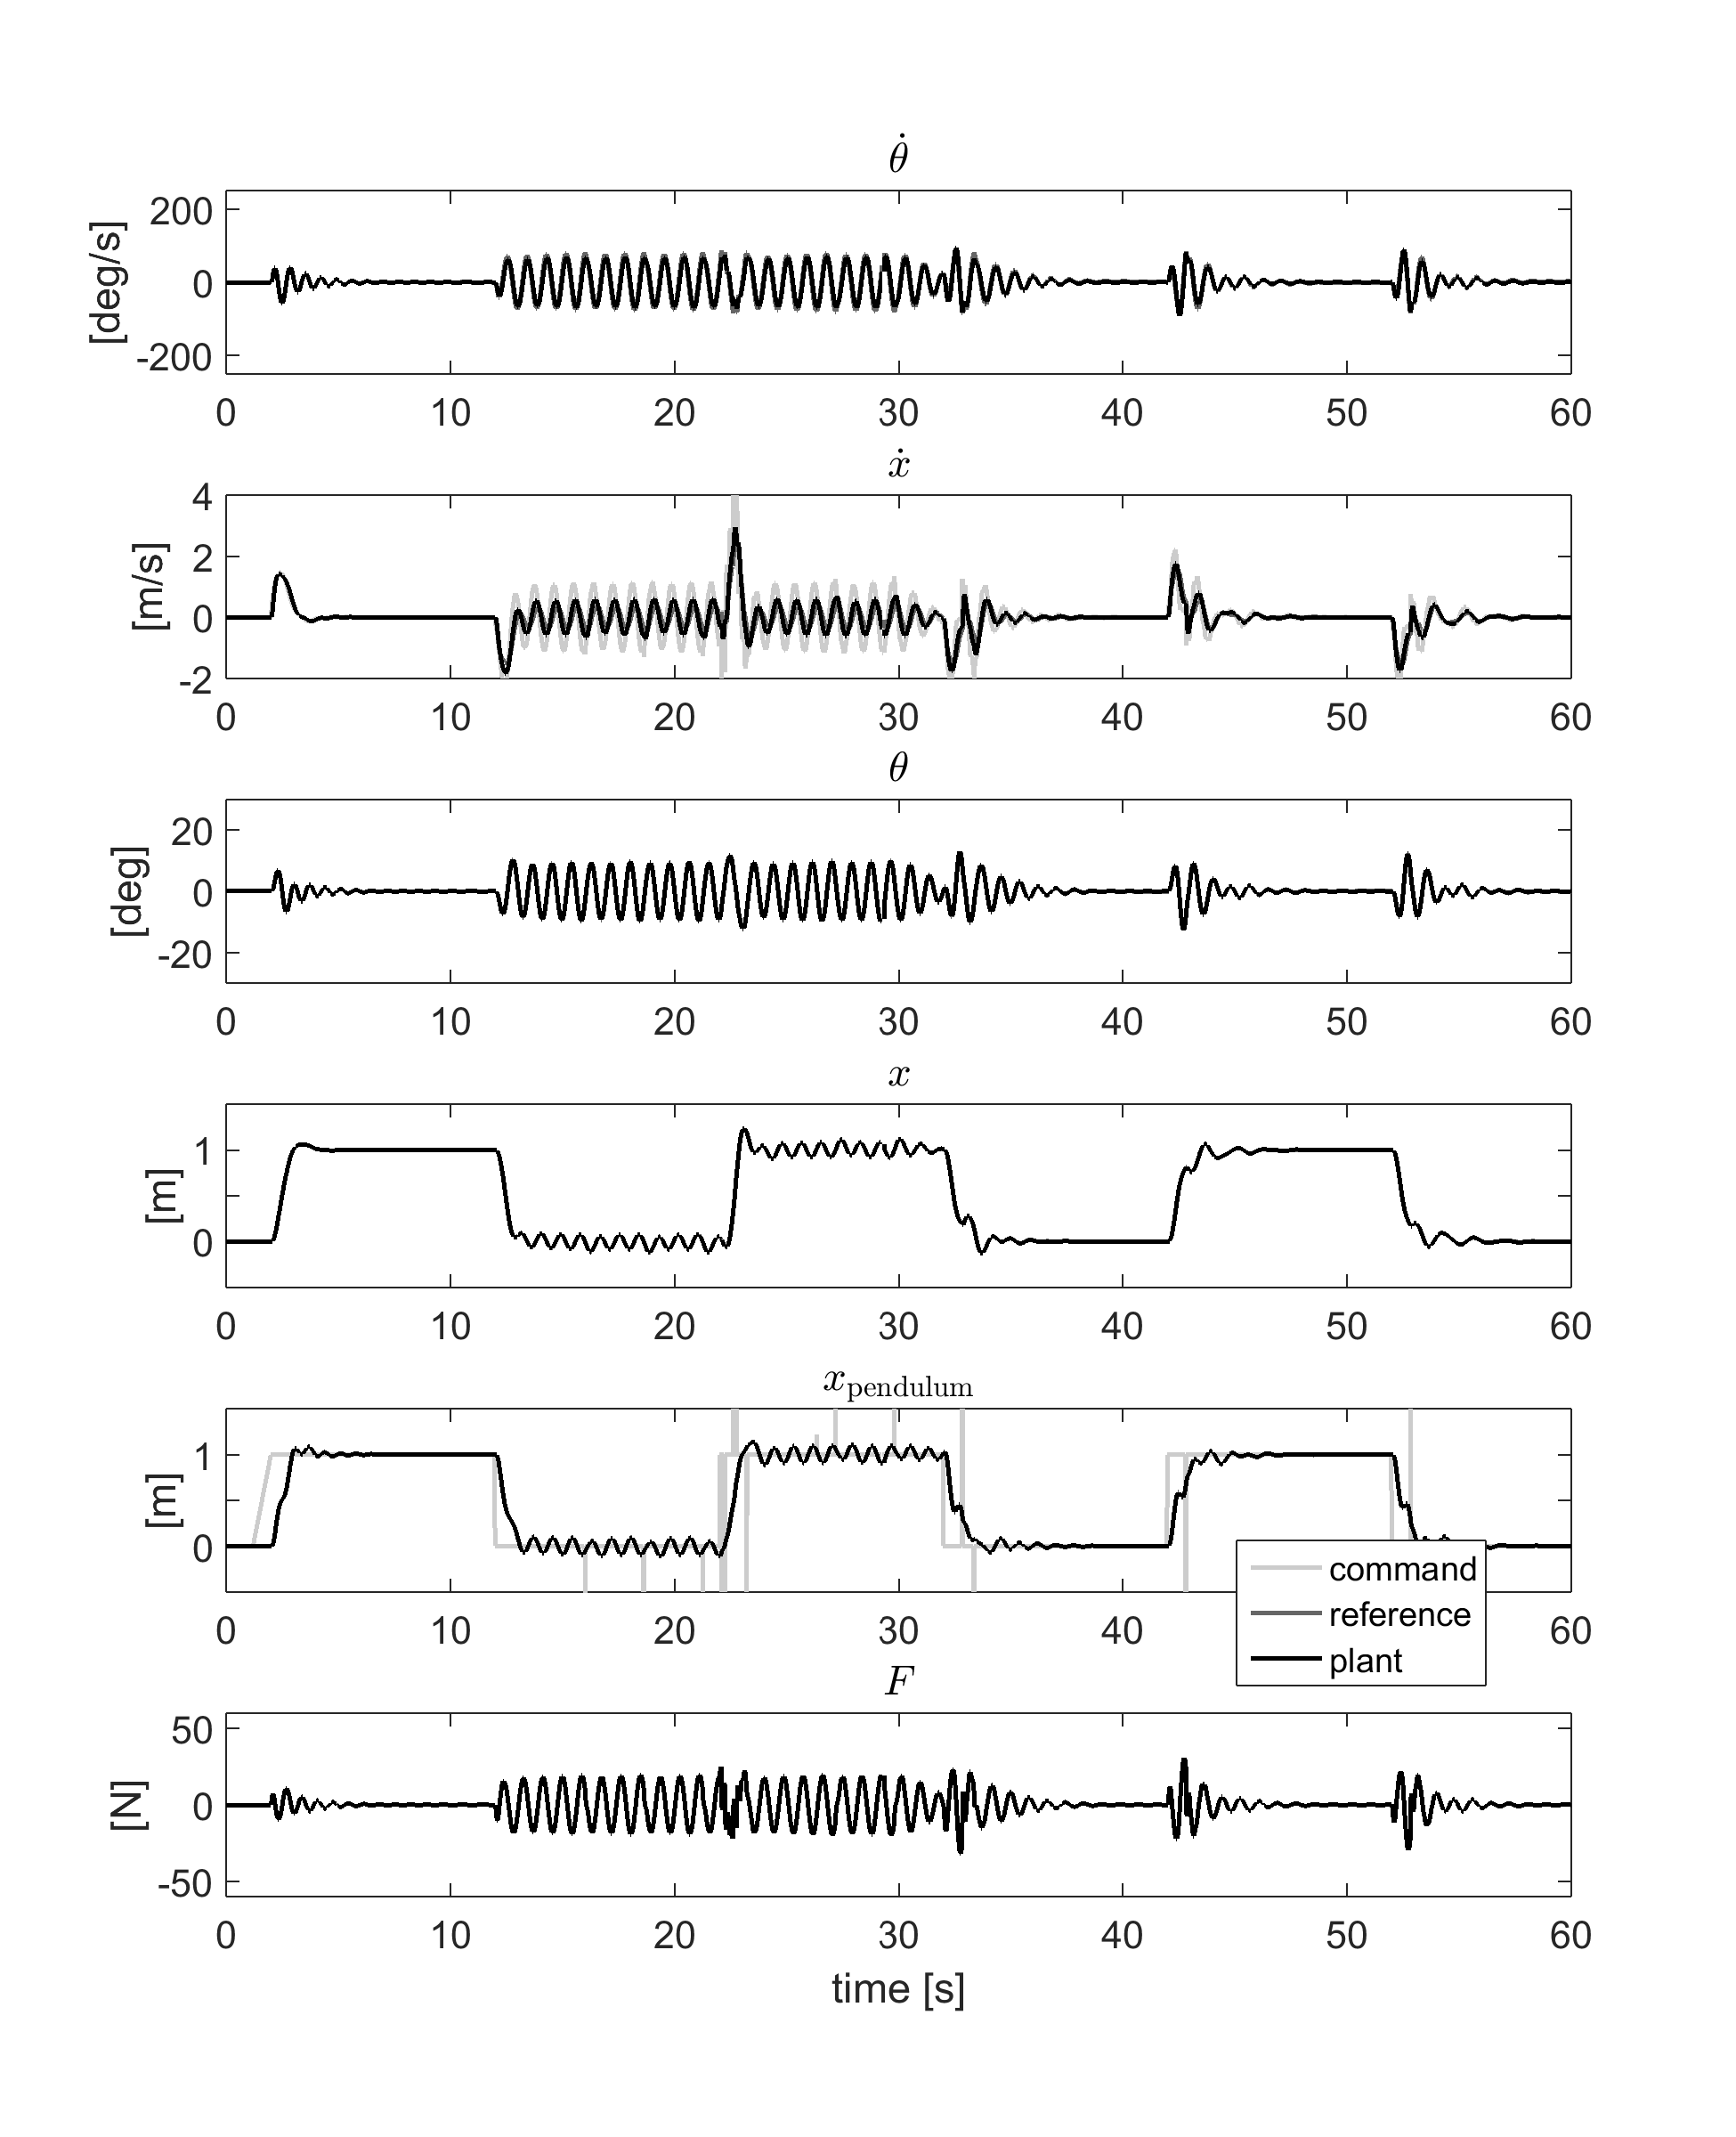
\includegraphics[width=7.0in]{\figurepath/outerLoopStateLimiterPendulumCart.png}}
  \vspace{-0.95in}
  \caption{Time response of pendulum cart with inner and outer-loop controller and state limiter.\label{fig.outerLoopStateLimiterPendulumCart}}
\end{figure}

\subsection{Example 2: Longitudinal Dynamics of a Transport Aircraft}

\begin{figure}[H]
  \begin{center}
    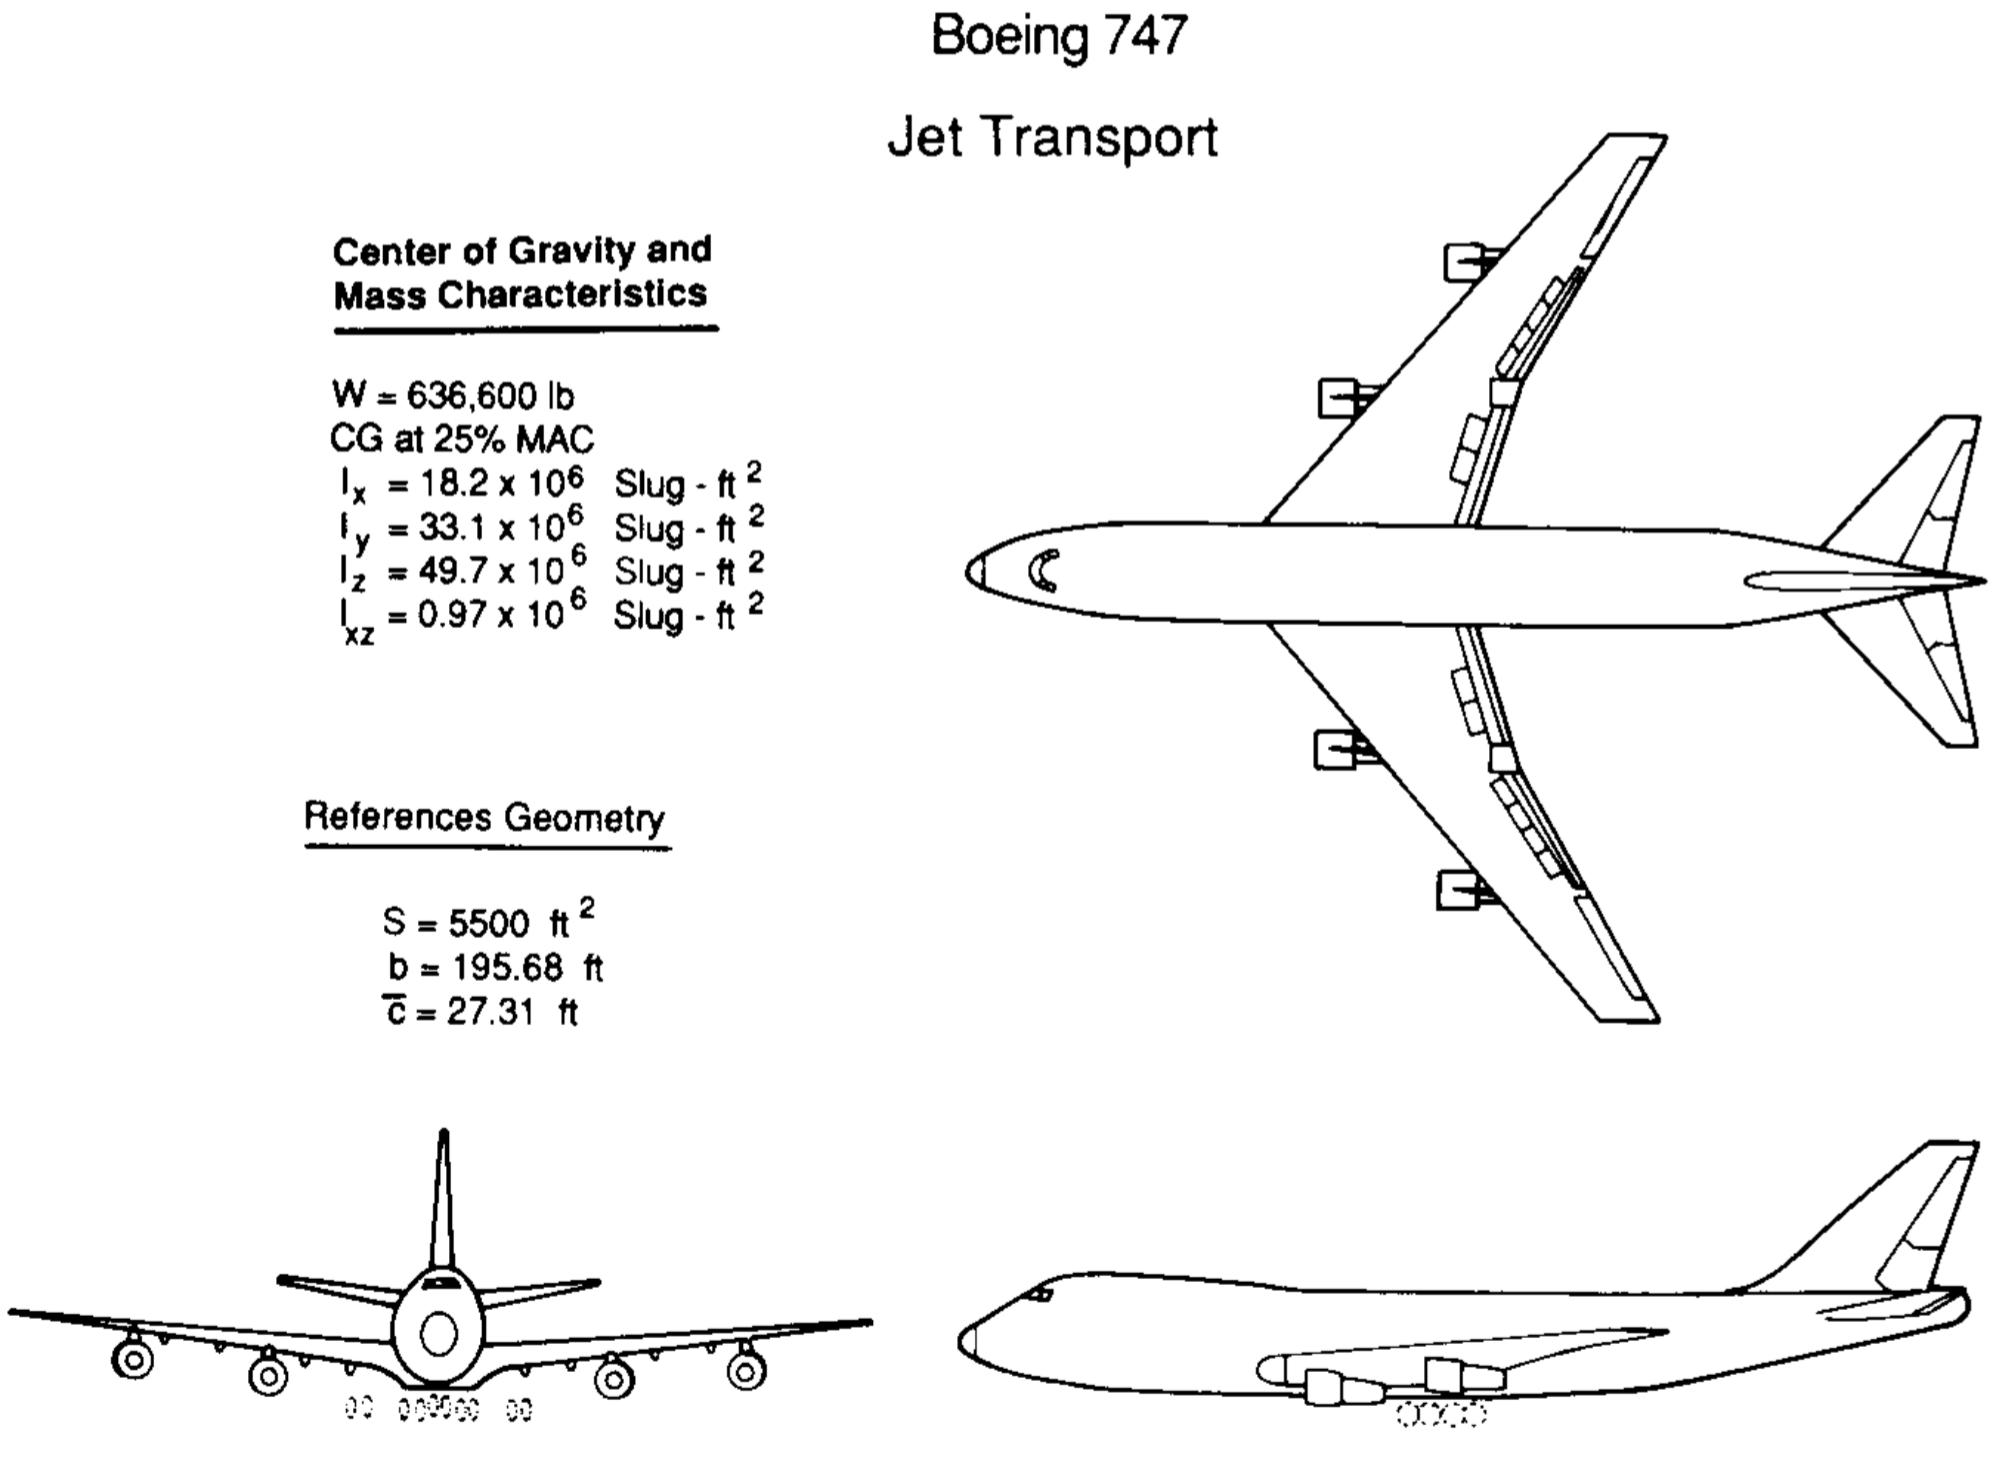
\includegraphics[width=4.5in]{\figurepath/transportLong.png}
    \vspace{-0.1in}
    \caption{Boeing 747--100 transport aircraft from Ref.\ \cite{nelson.flightcontrol.1998}.\label{fig.transportLong}}
  \end{center}
\end{figure}

The longitudinal dynamics of a transport aircraft example from Section~\ref{sec.innerLoopNumericalExample} is continued here.
In the first part of this example, the inner-loop adaptive controller was used to accommodate uncertainties in the moment coefficients and elevator effectiveness, and enforced tracking of the pitch rate commands.
The example is continued here using the plant with this adaptive inner-loop, and the outer-loop controller prescribe the necessary pitch rate command so as to track altitude commands.

The longitudinal aircraft dynamics in\ \eqref{eqn.transportAircraftWhole} were partitioned into the inner-loop dynamics in\ \eqref{eqn.transportAircraftInnerLoop} and the outer-loop dynamics in the form of\ \eqref{eqn.outerLoopDynamics} given in\ \eqref{eqn.transportAircraftOuterLoop} below
\begin{equation}
  \label{eqn.transportAircraftOuterLoop}
  \begin{split}
    \begin{bmatrix}
      \dot{\theta} \\
      \dot{h}
    \end{bmatrix}
    &=
    \begin{bmatrix}
      0 & 0 \\
      v_{\text{eq}} & 0 \\
    \end{bmatrix}
    \begin{bmatrix}
      \theta \\
      h
    \end{bmatrix}
    +
    \begin{bmatrix}
      0 & 1 \\
      -v_{\text{eq}} & 0 \\
    \end{bmatrix}
    \begin{bmatrix}
      \alpha \\
      q
    \end{bmatrix} \\
    h
    &=
    \begin{bmatrix}
      0 & 1
    \end{bmatrix}
    \begin{bmatrix}
    \theta \\
    h
    \end{bmatrix}
  \end{split}
\end{equation}
The matrix $B_{gd}$ which couples the outer-loop kinematics into the inner-loop dynamics in this example is identically zero.
Using the numerical values for the aircraft given in Section~\ref{sec.innerLoopNumericalExample}, the relevant matrices are given by
\begin{equation*}
  A_{g} =
  \begin{bmatrix}
    0 & 0 \\
    871 & 0
  \end{bmatrix}
  \qquad
  B_{gp} =
  \begin{bmatrix}
    0 & 1 \\
    -871 & 0
  \end{bmatrix}
  \qquad
  C_{g} =
  \begin{bmatrix}
    0 \\
    1
  \end{bmatrix}^{\top}
  \qquad
  C_{gz} =
  \begin{bmatrix}
    0 \\
    1
  \end{bmatrix}^{\top}
\end{equation*}
The forward-loop reference model was designed using integral action on the regulated output as in\ \eqref{eqn.rKbar} using the following weighting matrices
\begin{equation*}
  \begin{split}
    Q_{\text{lqr}}
    &=
    \text{diag}\bigr(
    \begin{bmatrix}
      0 & 10 & 0 & 0 & 10 & 10
    \end{bmatrix}
    \bigr) \\
    R_{\text{lqr}}
    &=
    10^{8}
  \end{split}
\end{equation*}
Using the outer-loop design procedure summarized in Section~\ref{sec.outerLoopDesignProcedureSummary}, $P_{g}$ was calculated as in\ \eqref{eqn.Pg} using $P$ calculated as in\ \eqref{eqn.P} and $X_{D}$, where $P_{\Lambda}$ in\ \eqref{eqn.P}, and $X_{D}$ was selected as
\begin{equation*}
  X_{D}
  =
  \begin{bmatrix}
    100 & 0 \\
    0 & 100
  \end{bmatrix}
  \qquad
  P_{\Lambda}
  =
  \begin{bmatrix}
    1 & 0 \\
    0 & 1
  \end{bmatrix}
\end{equation*}
With the resulting $P_{g}$, $S_{g}$ was determined using\ \eqref{eqn.SgCaseI}, and $L_{g}$ obtained numerically satisfying\ \eqref{eqn.condition4a}.
Finally $L_{y}$ was computed using\ \eqref{eqn.Ly} thus completing the outer-loop control design.

The following plot in Fig.~\ref{fig.outerLoopTransportLong} shows the response of the closed-loop system to track altitude commands, when subject to the same uncertainties described in Section\ref{sec.innerLoopNumericalExample}.
The plot shows the baseline controller applied to the nominal plant until $t=90$ seconds when the uncertainty is introduced.
At $t=110$ seconds the adaptive controller is turned on.
As in the inner-loop example, the adaptive element ensures stability in the presence of the uncertainty, and outer-loop command tracking is provided.
However, in Fig.~\ref{fig.outerLoopTransportLong} during the transients a pitch rate of 30 deg/s is experience.
In Fig.~\ref{fig.outerLoopStateLimiterTransportLong} the state limiter is used to enforce the pitch rate to within 15 deg/s.

\newpage
\begin{figure}[H]
  \hspace{-0.0in}
  \noindent\makebox[6.5in]{%
  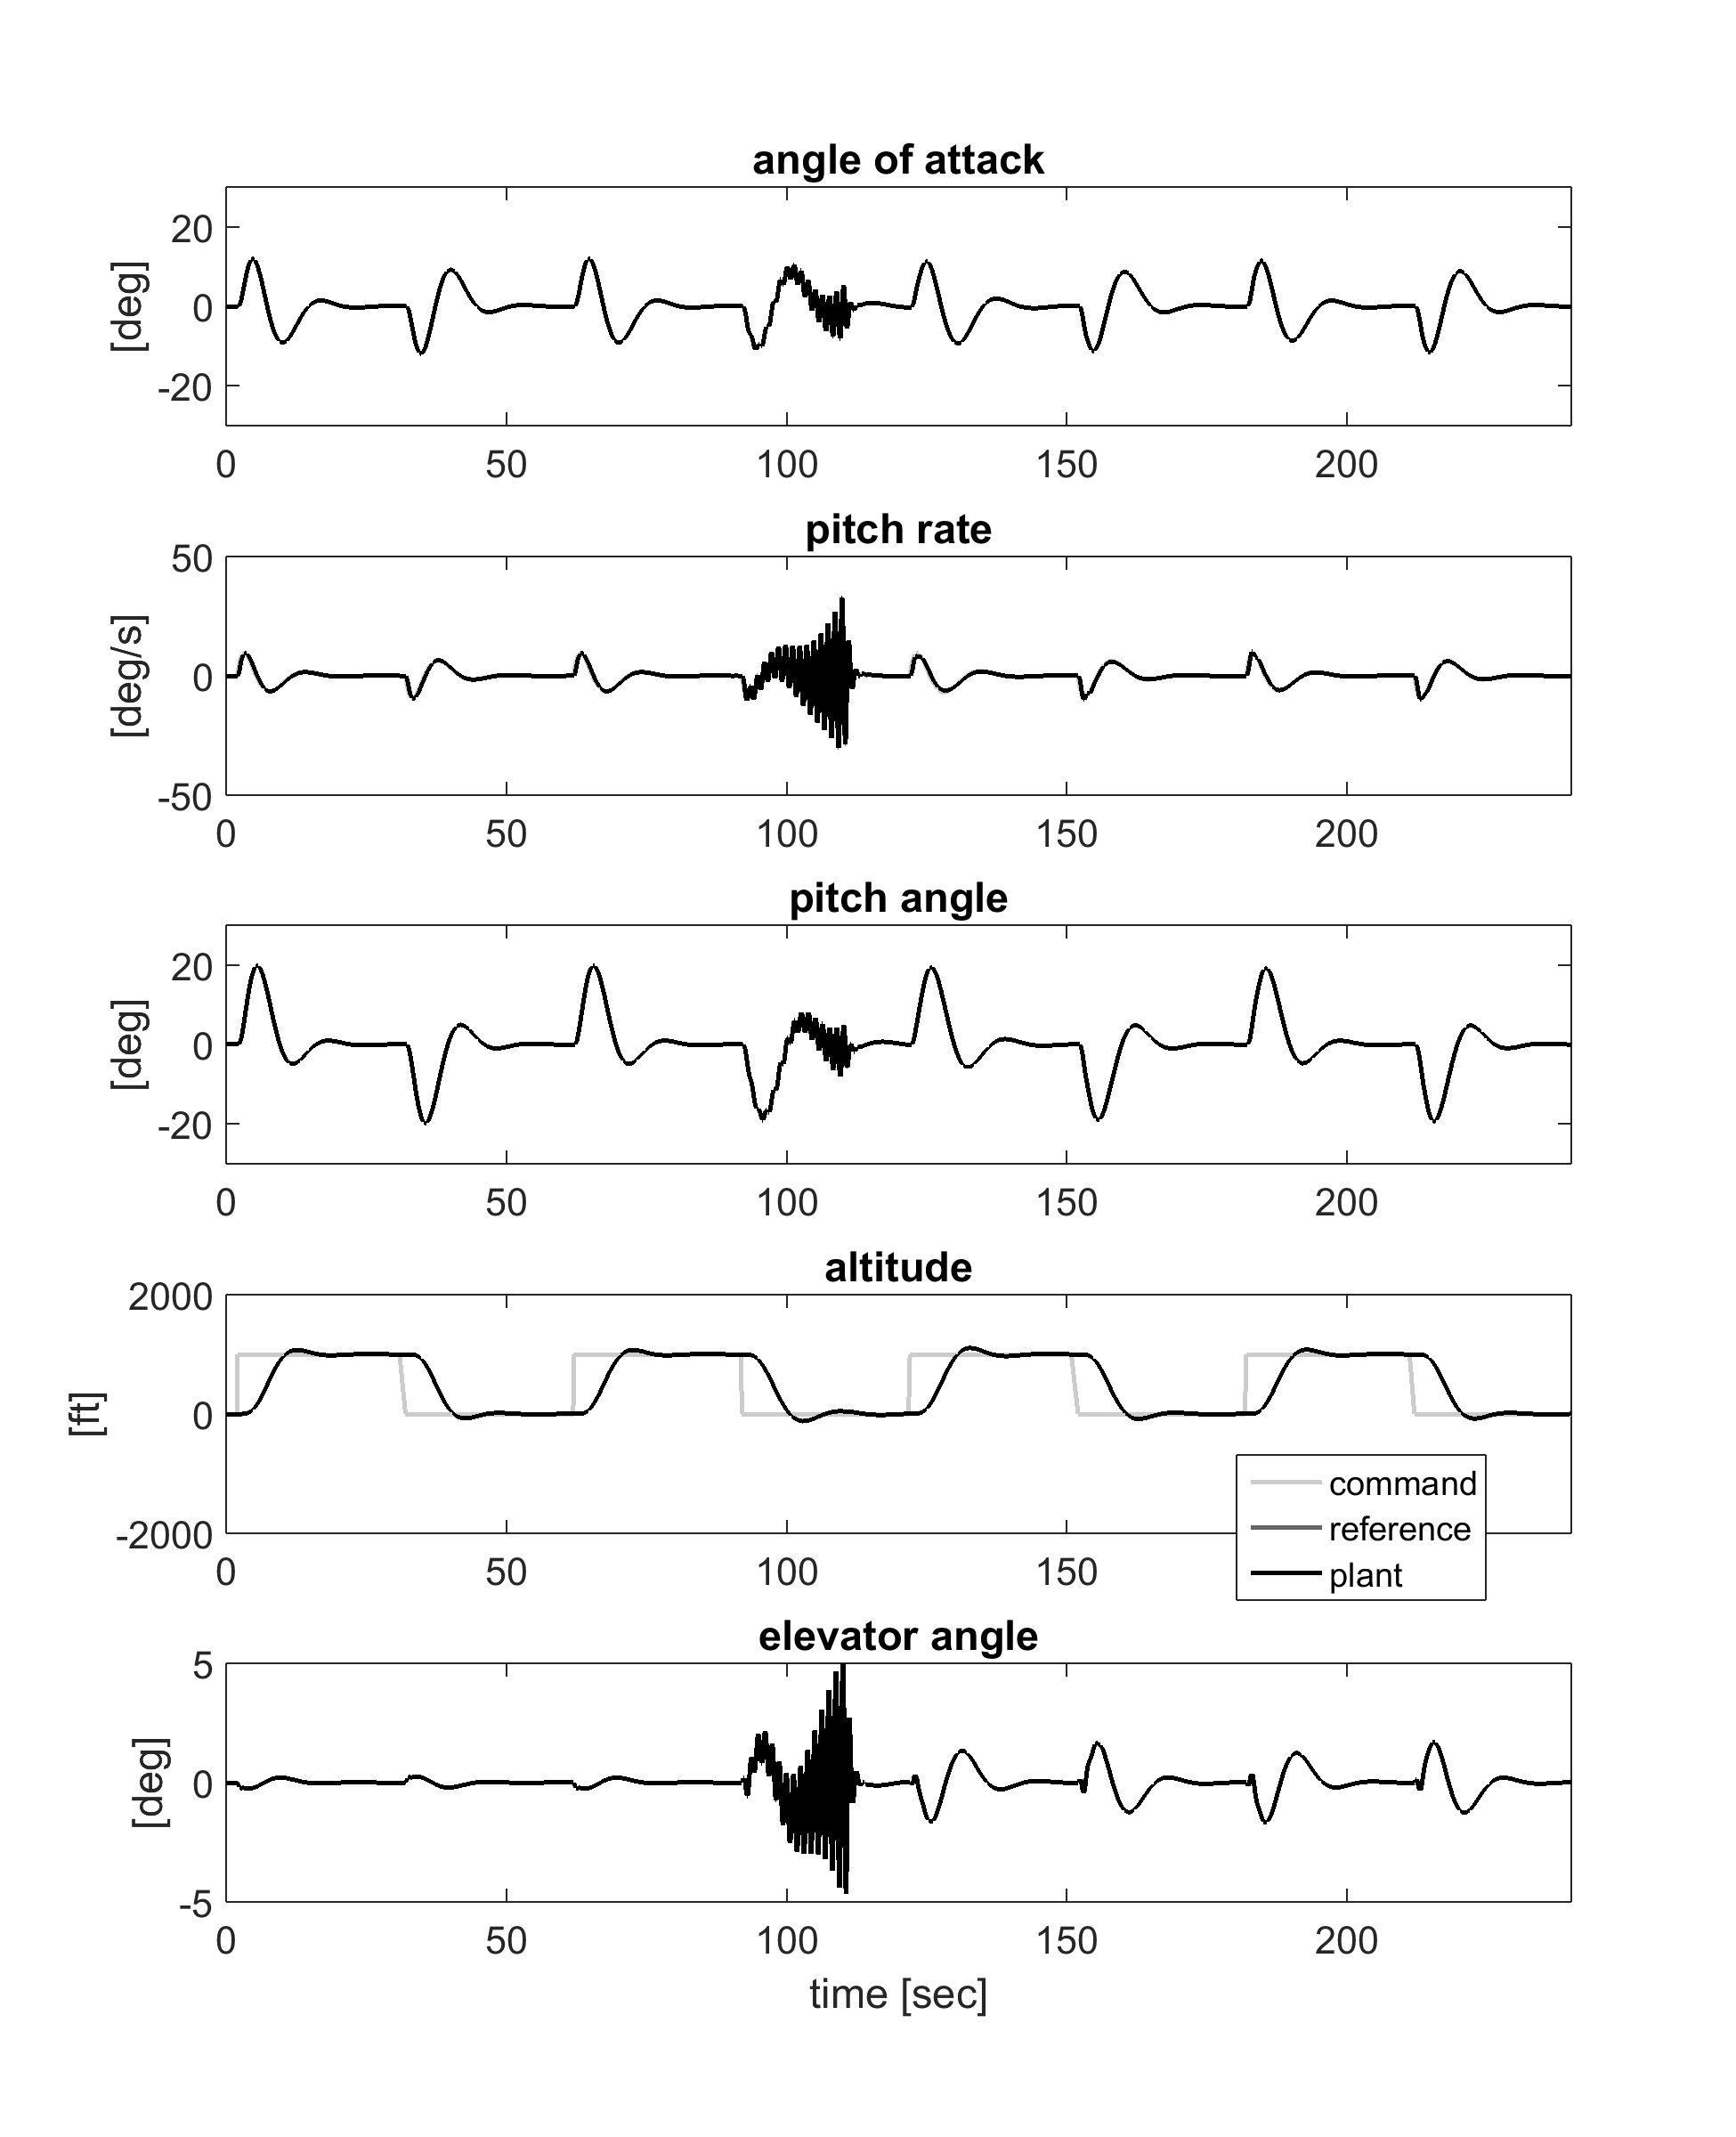
\includegraphics[width=6.5in]{\figurepath/outerLoopTransportLong.png}}
  \vspace{-0.95in}
  \caption{Time response of transport aircraft with inner and outer-loop controller.\label{fig.outerLoopTransportLong}}
\end{figure}

\newpage
\begin{figure}[H]
  \hspace{-0.0in}
  \noindent\makebox[6.5in]{%
  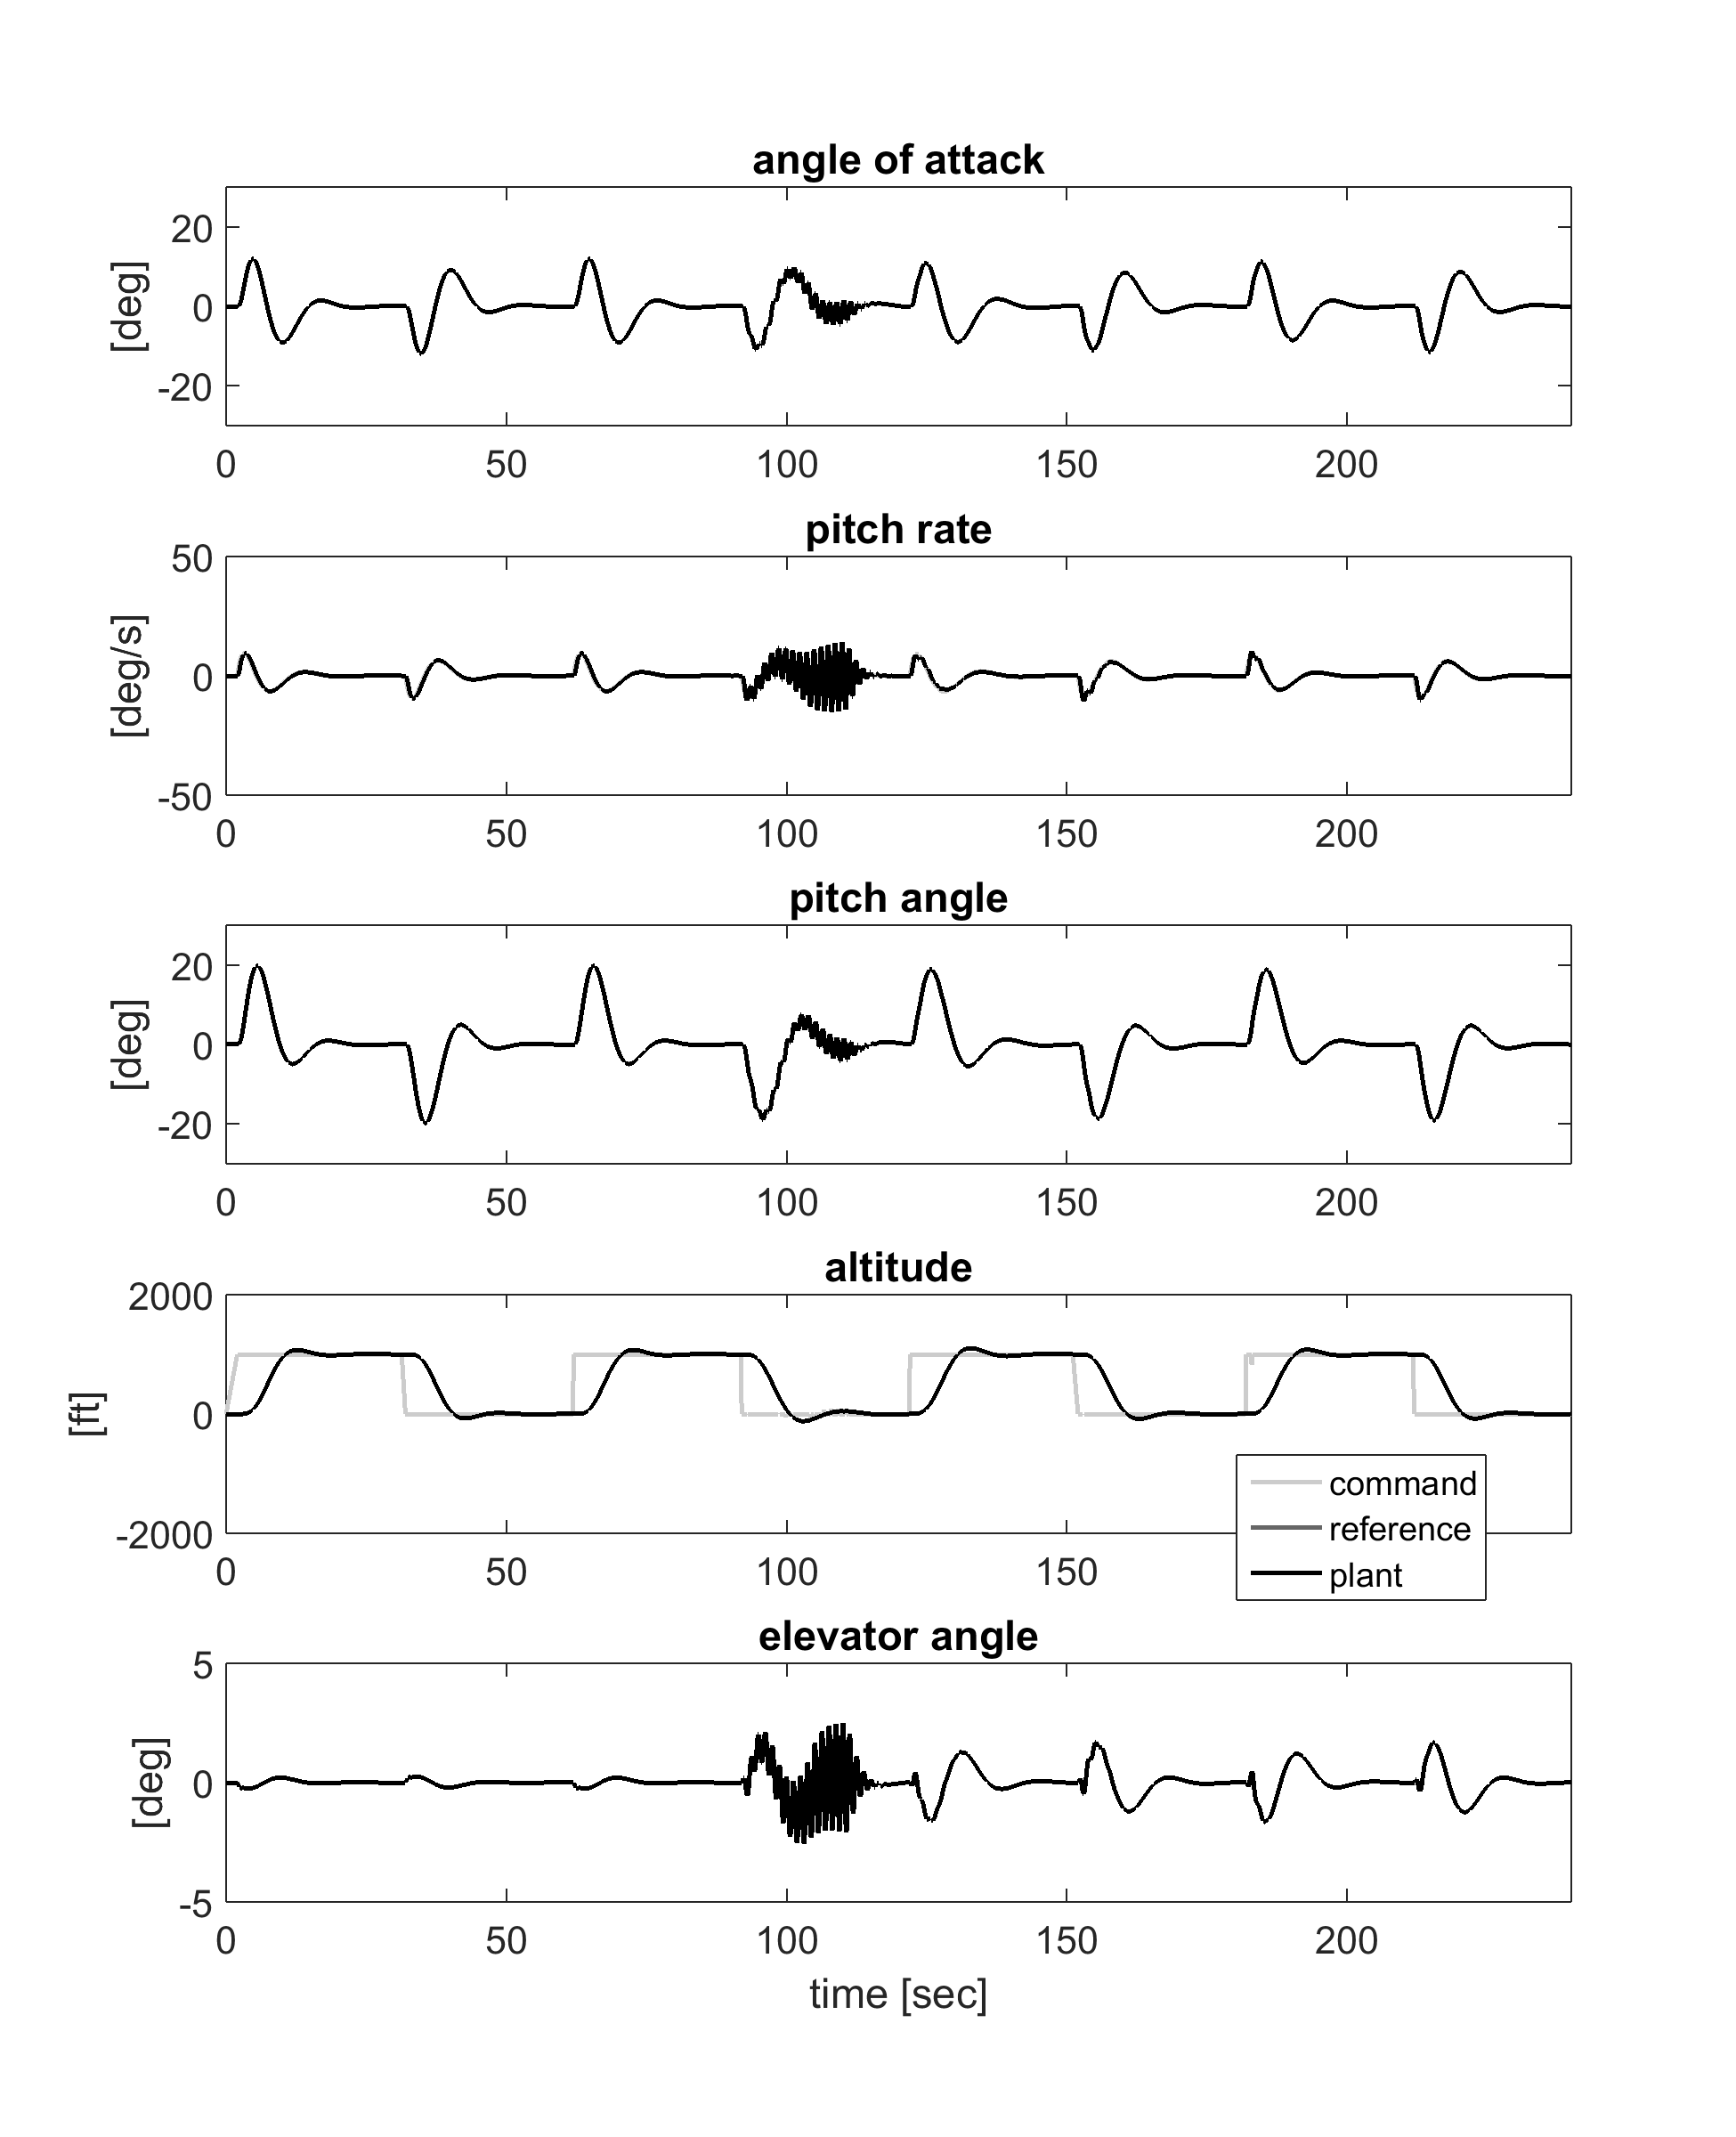
\includegraphics[width=6.5in]{\figurepath/outerLoopStateLimiterTransportLong.png}}
  \vspace{-0.95in}
  \caption{Time response of transport aircraft with inner and outer-loop controller and state limiter.\label{fig.outerLoopStateLimiterTransportLong}}
\end{figure}

\section{Conclusion}

This chapter presented a new method for developing an outer-loop controller for a class of uncertain MIMO systems.
Using the existing inner-loop adaptive control design presented in Ch.~\ref{ch.innerLoop}, this chapter described how to specify the command $z_{p,\text{cmd}}(t)$ to the inner-loop such that $z_{g}(t)$ tracks $z_{g,\text{cmd}}^{\prime}(t)$.
The controller is composed of additional reference model dynamics corresponding to the outer-loop dynamics, and additional CRM gains to suitably modify the outer-loop reference model trajectories to ensure global stability, and provide command tracking of the outer-loop command.
Specifically, these CRM gains were chosen so as to stabilize the outer-loop reference model, and then decouple the inner and outer-loop error dynamics.
Synthesis of the CRM gains involved satisfying a matrix equality and an bilinear inequality, to provide the desired error decoupling, and outer-loop reference model stability.
Using the matrix elimination lemma as in Ch.~\ref{ch.innerLoop}, the BMI was reduced to an LMI, and the problem of determining the CRM gains was reduced to finding a positive definite matrix $P_{g}$ which satisfied the LMI, with the additional constraint that $P_{g}$ also satisfy the matrix equation $\Pi_{A}P_{g}\Pi_{B}=\Pi_{C}$.
The set of all solutions which satisfied these constraints was given in terms of an arbitrary matrix $X_{D}$.
The set of all $X_{D}$ which ensured a stable outer-loop controller was large, allowing the extra degrees of freedom of $X_{D}$ to be selected to provide the desired level of performance and robustness to the closed-loop system, in addition to stability.
The result is a hierarchical MIMO adaptive output-feedback controller which can be designed to have good stability margins, contains an adaptive element to accommodate uncertainty, and provides the desired command tracking.
Furthermore, the architecture of the hierarchical approach allowed the addition of a state-limiter to the controller, to limit the plant state to certain regions in the state space.

In Ch.~\ref{ch.applicationHypersonic} this hierarchical, MIMO adaptive output feedback controller consisting of the inner-loop controller from Ch.~\ref{ch.innerLoop} and the outer-loop controller from Ch.~\ref{ch.outerLoop} is applied to a hypersonic vehicle model.

\chapter{Application to a Hypersonic Vehicle}\label{ch.applicationHypersonic}

\section{Introduction}

Some of the challenges associated with the control of hypersonic vehicles include the limited wind tunnel data available to determine accurate models for control design, large flight envelopes with significant uncertainty in the operating environment, and need to cope with engine unstart, in addition to problems such as actuator failure, flexibility effects, and time delays.
This section provides some background and historical context to hypersonic flight, discusses some of the existing methods developed to control hypersonic vehicles and cope with these challenges, and why the adaptive control structure used in this thesis was chosen.

In this chapter the efficacy of the proposed combined inner and outer-loop control design method described in Chapters~\ref{ch.innerLoop} and~\ref{ch.outerLoop} is examined by providing a numerical example.
An adaptive output feedback controller following this sequential loop closure process is designed and applied to the a 6-DOF Generic Hypersonic Vehicle model\ \cite{wiese.adaptive.2013, rollins.nonlinear.2013, wiese.gnc.2015, wiese.jgcd.2015}.
The GHV is a small blended wing-body vehicle, with 3-D inlet and nozzle, and axisymmetric through-flow scramjet engine.
The nonlinear equations of motion describing the GHV are linearized about a nominal flight condition of Mach 5 at an altitude of 80,000 feet, corresponding to a dynamic pressure of 1,474 lb/ft$^2$.
Modal analysis allowed the linearized equations of motion to be decoupled, and the resulting uncertain longitudinal and lateral-directional plant subsystems are represented as in Eq.\ \eqref{eqn.wholeSystemUncertain}, and velocity dynamics represented as in\ \eqref{eqn.xdotpunc}.
These uncertain linear subsystems compose the design model which is used to synthesize the controller.

In Reference\ \cite{wiese.adaptive.2013} a \textit{state feedback} LQR baseline controller with integral action and augmented with an adaptive component was applied to design three independent CRM based adaptive controllers\textemdash{}one for the each of the longitudinal, lateral-directional, and velocity subsystems.
In Ref.\ \cite{wiese.sequential.2016} the outer-loop design described in Ch.~\ref{ch.outerLoop} was presented for the state-feedback case as well, given by\ \eqref{eqn.wholeSystemUncertain} where $C_{p}=I$ and $C_{g}=I$, and implemented on the linear longitudinal dynamics of the GHV with a state-feedback inner-loop as in\ \cite{wiese.adaptive.2013}.
This approach was very effective at maintaining stability and tracking performance in the presence of uncertainty, but required the availability of angle-of-attack and sideslip angle measurements.

In the following example, it is no longer required that these incidence angles are measurable, which is more realistic for this class of vehicle, thus turning the problem into one of output feedback.
That is, $C_{p}\neq I$ and $C_{g}\neq I$ in\ \eqref{eqn.wholeSystemUncertain}.
The adaptive control design procedure described in Chapter~\ref{ch.innerLoop} was used to design two independent CRM based inner-loop \textit{output feedback} adaptive controllers, one for each of the longitudinal and lateral-directional subsystems, with a state-feedback controller used for the velocity subsystem.
The outer-loop output feedback controller described in Ch.~\ref{ch.outerLoop} was used around the longitudinal and lateral subsystems with inner-loop controller.
This sequential loop closure based adaptive output feedback controller is then applied to the evaluation model, which is nonlinear, coupled, and includes actuator dynamics, and is shown to result in stable tracking in the presence of uncertainties that destabilize the baseline linear output feedback controller.

\subsection{Background}

With a history spanning well over a half century, hypersonic flight continues to be a topic of significant research interest\ \cite{brocanelli.unstartrecovery.2012, dalle.envelope.2011, gibson.adaptive.2009, kothari.reusable.2010, parker.control.2007}.
Air-breathing hypersonic vehicles are particularly attractive due to their potential to serve as high speed passenger transports and long range weapon delivery systems, and provide cost-effective access to space.
Hypersonic vehicles are likely to be inherently unstable\ \cite{bolender.hypersonicmodel.2007, mcruer.hypersonic.1991, mirmirani.airbreathing.2005} and the integration of the airframe and engine in an air-breathing hypersonic vehicle contributes to additional modeling and control challenges.
With limited wind tunnel data, harsh and uncertain operating environments, poorly known physical models, and largely varying operating conditions, it is of great importance to ensure that any control scheme will be significantly robust to ensure safe operation during flight.

Unlike the transition from subsonic to supersonic flow, the physics of hypersonic flow do not differ from that of supersonic flow.
Instead, the distinction of hypersonic flow is made to stress the importance of certain physical phenomena which exist in all supersonic flows that become dominant at hypersonic speeds, typically defined to be flow at a Mach number of 5 or greater\ \cite{anderson.aerodynamics.2010}.
It wasn't until 1946, well into the study of such flow regimes, that this term was finally coined\ \cite{Tsien2012443}.
The high flight Mach numbers experienced by a hypersonic vehicle result in significant aerodynamic heating.
This aerodynamic heating can have a great impact on the material properties of the vehicle.
In addition to this coupling of aerodynamic and structural effects, the engines of air-breathing hypersonic vehicles are tightly integrated into the airframe of the vehicle, where long fore and aft sections of the vehicle make up large portions of the engine inlet and nozzle, respectively.
This tightly couples the engine dynamics with the airframe and structural dynamics as well as the aerodynamics\ \cite{chavez.flightdynamics.1994}.
The physics of hypersonic flow and these resulting interactions between all the components of the vehicle make the control of hypersonic vehicles very challenging.

A major challenge associated with the control of hypersonic vehicles, in addition to the interactions between airframe, engine, and structural dynamics, is the limited ability to accurately determine the aerodynamics characteristics\ \cite{chavez.analytical.1994, coleman.hypersonic.2009, maughmer.prediction.1989, schmidt.dynamics.1991}.
With the presence of such tight coupling between all aspects of a hypersonic vehicle, the ability to collect wind tunnel and flight data to study these interactions would be highly useful.
However, these tests are very difficult to do, and so much of the knowledge about a hypersonic vehicle's aerodynamics must come from physics-based models.
This makes accurate determination of the aerodynamic characteristics very difficult, making the design of a controller more difficult as well.

Another control challenge associated specifically with air breathing hypersonic vehicles is that of engine unstart.
Unstart is a phenomenon caused by several factors including thermal choking and insufficient air recovery at the inlet.
This ultimately leads to the upstream propagation of the shock train out of the inlet, effectively preventing air from entering the engine due to a standing normal shock in front of the isolator entrance\ \cite{curran.scramjet.2000}.
This causes an abrupt change in the pitching moment, an increase in drag, decrease in lift, loss of thrust, and potentially changes in vehicle yawing and rolling moments as well\ \cite{bolender.unstart.2009}.
If the flight path is such that it requires the air-breathing hypersonic vehicles to encounter periods of unstart, the control law must be such that it can accommodate these large and sudden changes, thus ensuring stable flight can be maintained.

With all of the complex interactions between the different aircraft components, and high level of uncertainty in the models, the control of a hypersonic vehicle is very challenging.
These challenges have led to many advances in the design of flight control.

\subsection{History}

The science of aerodynamics was first invented in the early 1900s by Ludwig Prandtl in Germany.
The field of aerodynamics matured considerably over the next half-century, and during World War II, the Germans were beginning to approach hypersonic speeds in laboratory wind  tunnel tests at Mach 4.4, and with weapons such as the V-2 rocket approaching similar speeds\ \cite{heppenheimer.heatbarrier.2009}.
The hypersonic technology of the United States was substantially behind that of the Germans at the time, until the war ended and Wernher von Braun and his team of rocket scientists came to the United States.
Just over eleven years after the end of World War II, history was made when the X-2 became the fastest airplane ever, reaching a speed of almost Mach 3.2.
Moments after the record was broken, the plane lost control and began tumbling downwards toward Earth, destroying the plane and killing the pilot due to a mechanism known as inertial coupling\ \cite{nelson.flightcontrol.1998}.
This disaster made the consequences of not maintaining stability during high speed flight very real.

The study of hypersonics in the 1950s was also being propelled by the United States' interest in intercontinental ballistic missiles, which began with the X-17 rocket.
The accurate guidance of such missiles over long ranges was of particular importance, but it was the challenges associated with significant aerodynamic heating upon atmospheric re-entry that dominated research in this area during this time.
The first test of the X-17 took place in 1956 to investigate the re-entry of a hemispherical nose-cone, and reached a speed of Mach 12.4.
This research provided valuable information used in the Mercury program, which succeeded in putting the first American in space in 1961.
The inherently stable design of the Mercury capsule allowed safe atmospheric re-entry even without an effective control system.
While guidance, navigation and control (GNC) challenges of later hypersonic re-entry vehicles were more difficult, the effective control of atmospheric hypersonic vehicles such as the X-2 was a major problem that needed to be solved.

Following the testing of the X-2, the X-planes program continued in the late 1950s, with much of the knowledge gained through research to be used in the development of high performance fighter aircraft of the time.
One of the most notable hypersonic airplanes to ever fly, the X-15 pictured in Figure~\ref{fig:x15flying}, made its first flight in 1959.
The designers of the X-15 overcame many of the challenges associated with hypersonic flight.
The X-15 had to be very heat resistant to withstand the temperatures encountered during flight at nearly Mach 7, and the engine needed the power to propel the plane to these high speeds.
The flight envelope of the X-15 was so broad that reaction controls were used in addition to the aerodynamic control surfaces, which lost effectiveness above 100,000 feet altitude.
Transitioning between these two control systems was difficult as well.
In addition to these challenges, and more, the only significant source of aerodynamic data used in the development of the X-15 came from a single small hypersonic wind tunnel, making modeling for control especially challenging.
Despite these challenges, three variants of the X-15 made a combined total of nearly 200 flights over the next ten years following its first flight.
The third variant of the X-15 was the only of the three craft to include an adaptive controller as part of its stability augmentation system.
This adaptive controller attempted to adjust feedback gains to provide optimum angular rates as commanded by the pilot, and also provided a means to transition from aerodynamic to reaction controls.
Conventional aerodynamic control surfaces were used to create the moments necessary to control the vehicle when the atmosphere was sufficiently dense, but at high altitudes these surfaces lost their effectiveness, and a reaction control system using thrusters was required to create the necessary moments.
It was critical to allow the command of both control systems from a single control stick in the cockpit.
While the X-15 allowed hours of valuable flight data to be obtained, engineers were once again reminded of the consequences of faulty designs when the MH-96 adaptive controller aboard the X-15 failed to reduce the feedback gains upon re-entry, setting up a violent pitch oscillation which destroyed the aircraft and killed the pilot.

 \begin{figure}[h]
  \begin{center}
    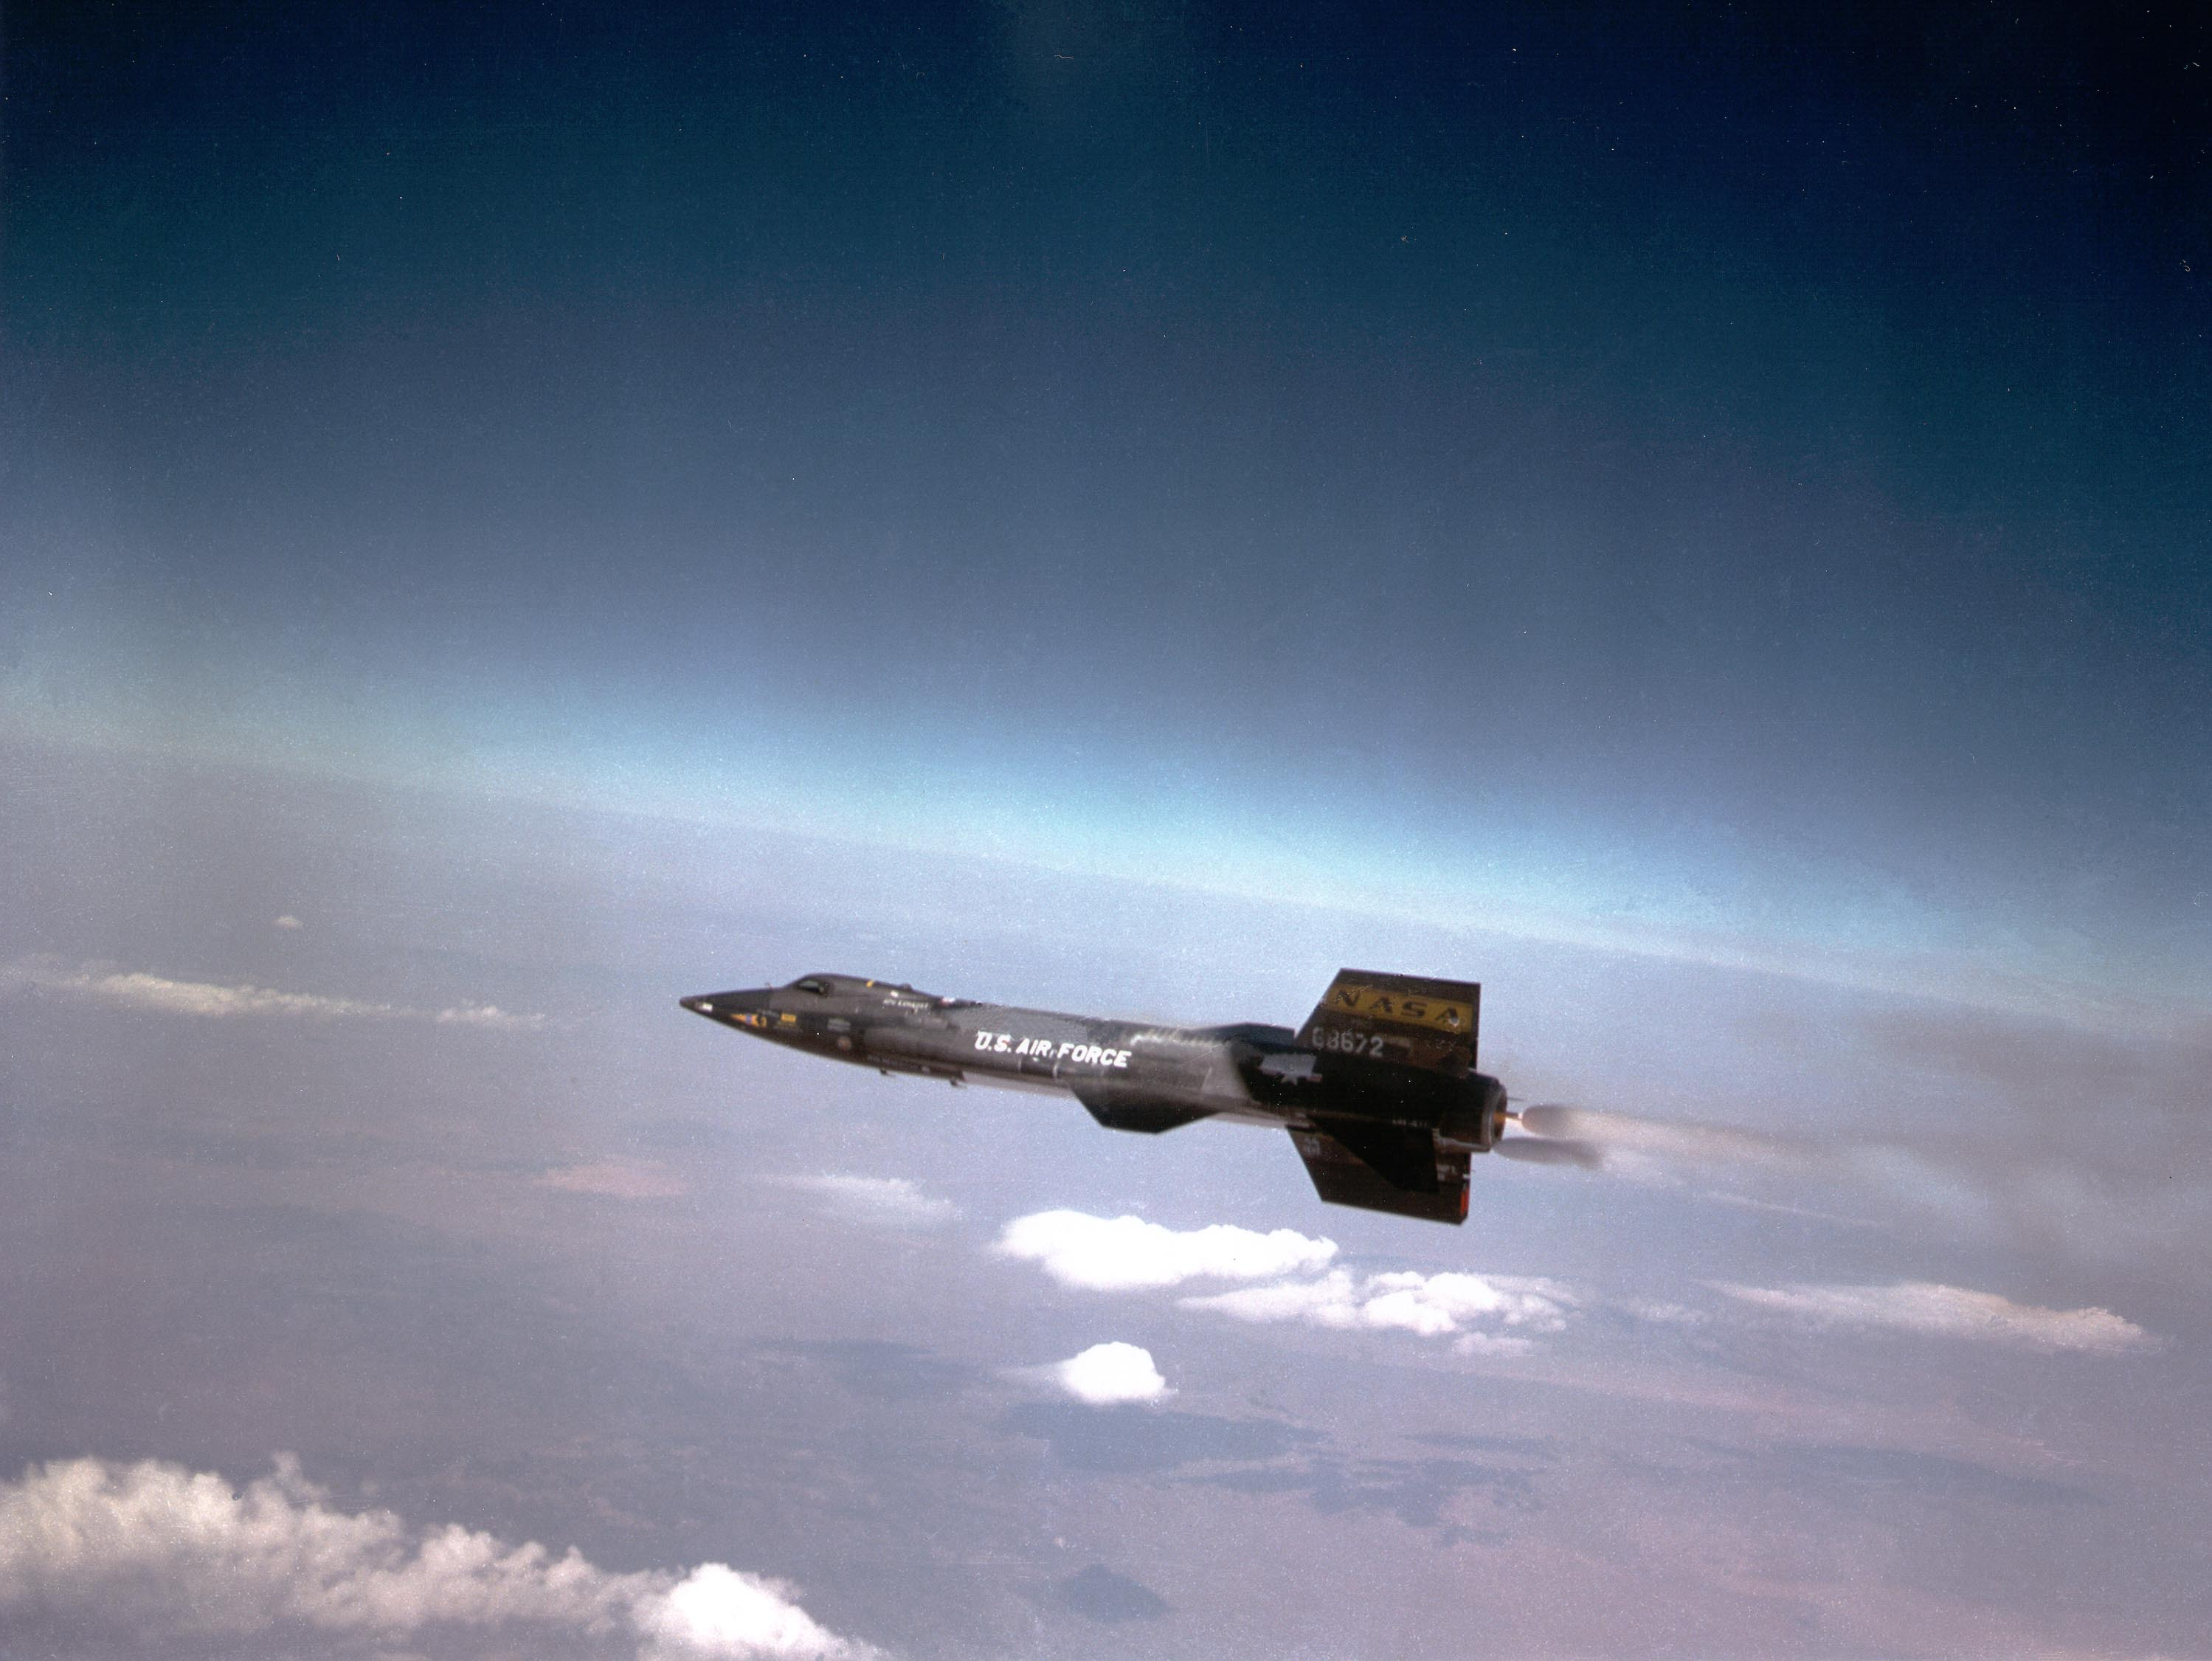
\includegraphics[width=3.5in]{\figurepath/x15flying.jpg}
    \caption{North American X-15 from Ref.\ \cite{x15picture}.\label{fig:x15flying}}
  \end{center}
\end{figure}

Toward the end of the X-15's career, there was a building interest in a new, advanced air-breathing propulsion system for hypersonic flight, as opposed to the rocket propulsion used on the X-15 and its predecessors.
This Hypersonic Research Engine (HRE) was to utilize concepts first disclosed by The Johns Hopkins Universities' Applied Physics Lab in 1959, as part of a project known as Supersonic Combustion Ramjet Missle (SCRAM).
The scramjet engines were initialy designed as pods, much like conventional turbofans on commercial and transport aircraft.
Early plans called for a podded scramjet to be fitted on the X-15, but it was quickly realized that this would not be possible.
To make scramjets practical for use in flight, the engine would have to be integrated intimately with the airframe, using the fore and aft sections of the vehicle as part of the inlet and nozzle of the scramjet.
Development of scramjet technology was pushed forward in the early 1980s in part by the U.S. Air Force, in order to develop a single-stage-to-orbit vehicle to deliver military weapons systems to space.
This ultimately led to the National Aero-Space Plane (NASP) program, and the design of the 160 foot long Rockwell X-30.
This program lasted over ten years and lead to many advances in scramjet propulsion research and the study of flexible hypersonic vehicles, but none of these vehicles were ever built.

\begin{figure}[h]
  \begin{center}
    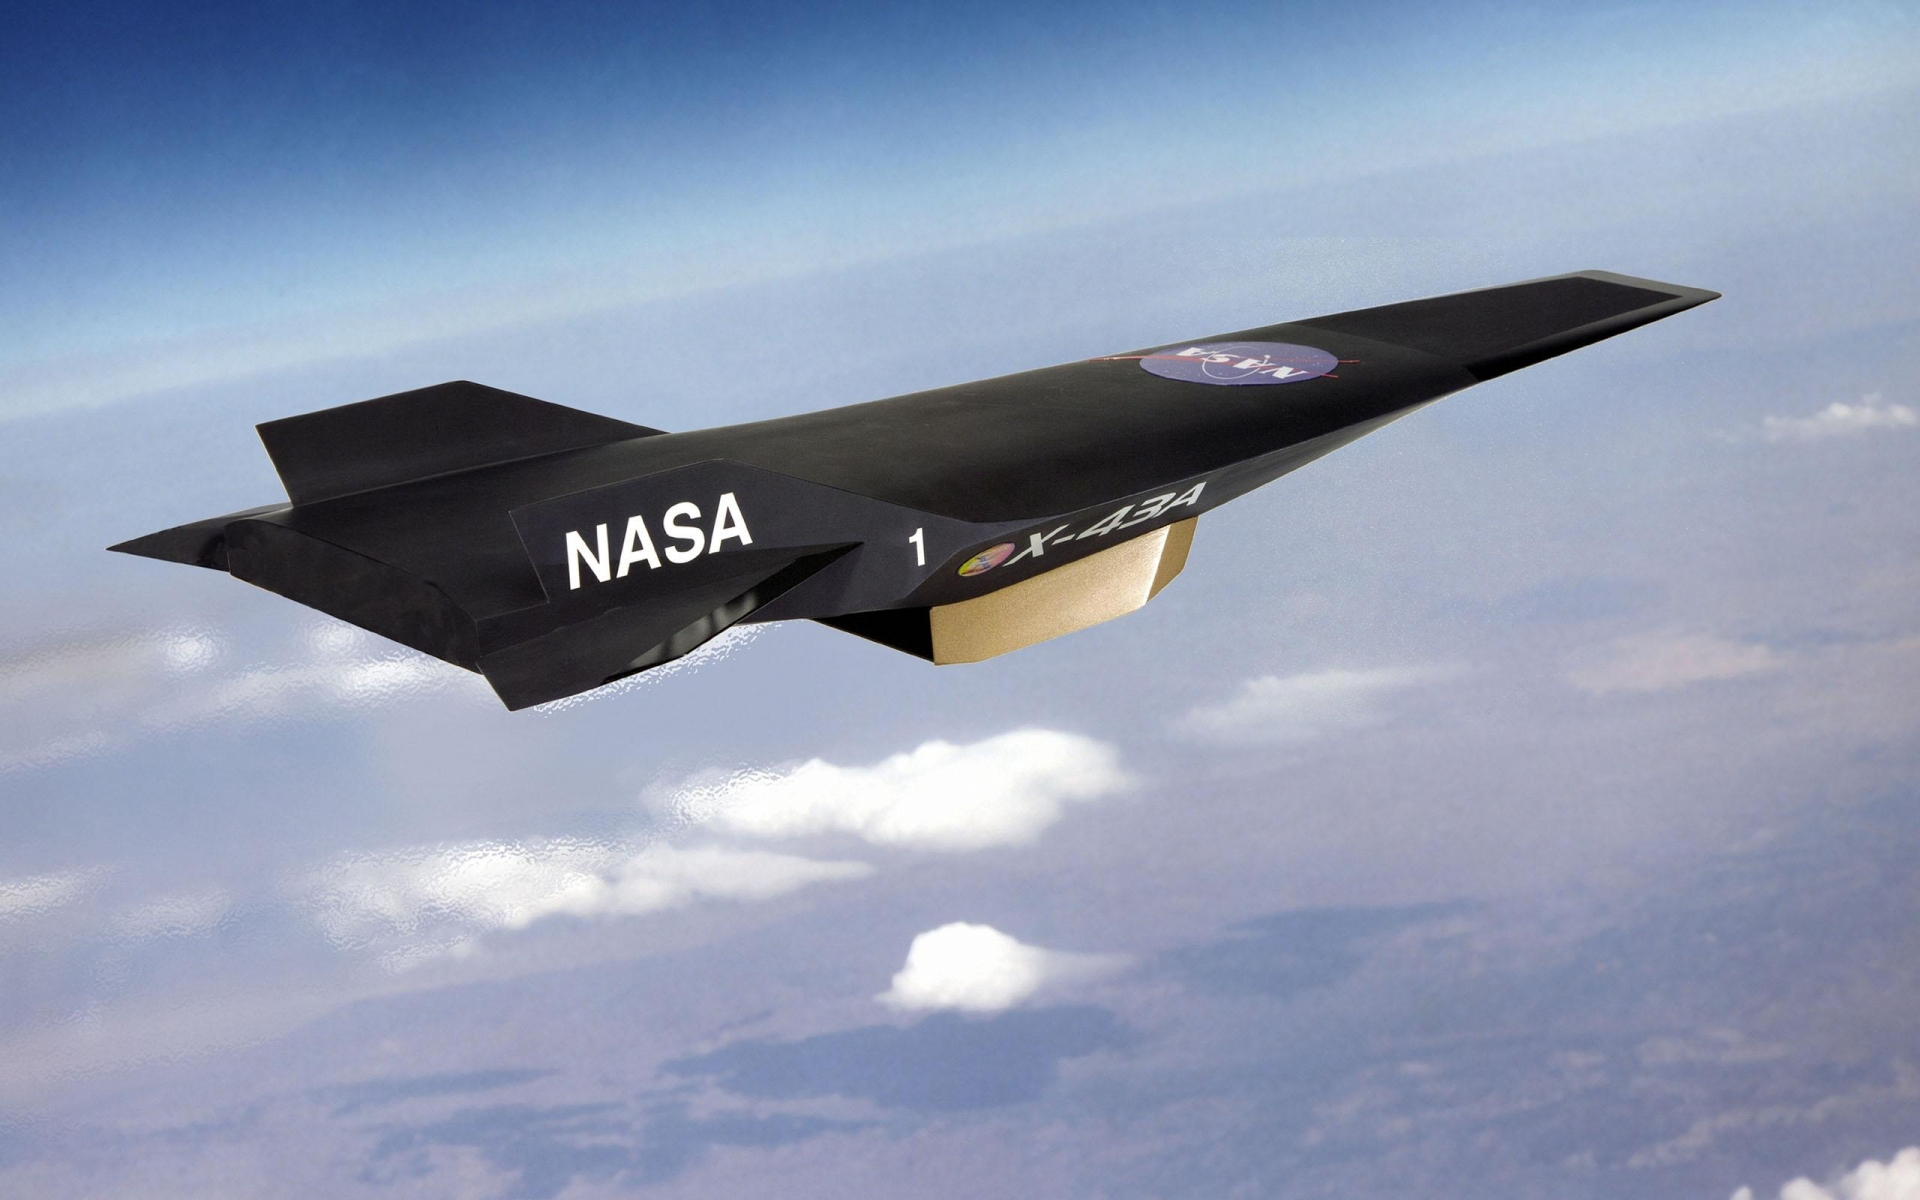
\includegraphics[width=3.5in]{\figurepath/nasa_x43.jpg}
    \caption{NASA X-43A from Ref.\ \cite{x43picture}.}
  \end{center}
\end{figure}

Hypersonic research slowed for some years, until scramjet research emerged again in the early 1990s as part of a collaboration between the United States and Russia.
This collaboration saw scramjets mounted aboard rockets being tested in flight.
Control again became a critical challenge in hypersonic flight, this time in the control of the engines.
Fuel delivery had to be controlled precisely to keep the engines operating in supersonic combustion mode, and avoid a condition known as unstart.
Control systems aboard these rocket-mounted scramjets were designed to monitor pressures within the engines and adjust fuel flow to prevent unstart, but the early control systems were not yet ready for this demanding challenges.
An all-American effort at practical scramjet powered hypersonic flight was born in 1996 under the name Hyper-X\ \cite{freeman.hyperx.1997}.
Hyper-X was an eight year NASA program with the goal of demonstrating the viability of air-breathing hypersonic flight.
The demonstrator vehicle for this program, the X-43, was 12 feet long, and 5 feet wide.
The first flight took place in June 2001 and failed, but in March 2004 the X-43A became the first vehicle to ever be propelled during hypersonic flight by an air-breathing engine, reaching a speed of Mach 6.8 for 11 seconds.
The third flight in November 2004 lasted 10 seconds and reached a speed of Mach 9.6.
These ground breaking flights demonstrated the practicability of a scramjet powered hypersonic vehicle, and are alongside the X-15 in terms of importance in the history of hypersonic flight.

In the 1990s and 2000s, many hypersonics programs have been introduced, including HyTECH, HyShot, HyCause, HIFiRE, and more.
The most notable platform since the X-43A was the X-51, built by Boeing and managed by the U.S. Air Force Research Lab (AFRL).
While the X-43A demonstrated the feasibility of scramjet powered flight, a new record was set by the X-51 in 2010 by maintaining scramjet powered flight at Mach 5 for 140 seconds.
The second X-51 flight took place in 2011 and ended early due to unstart, and during the third test flight the X-51 lost control and fell into the ocean.
History was made once again in May 2013, when the X-51 made the longest air-breathing hypersonic flight, maintaining Mach 5.1 for 240 seconds under its own power.

\begin{figure}[h]
  \begin{center}
    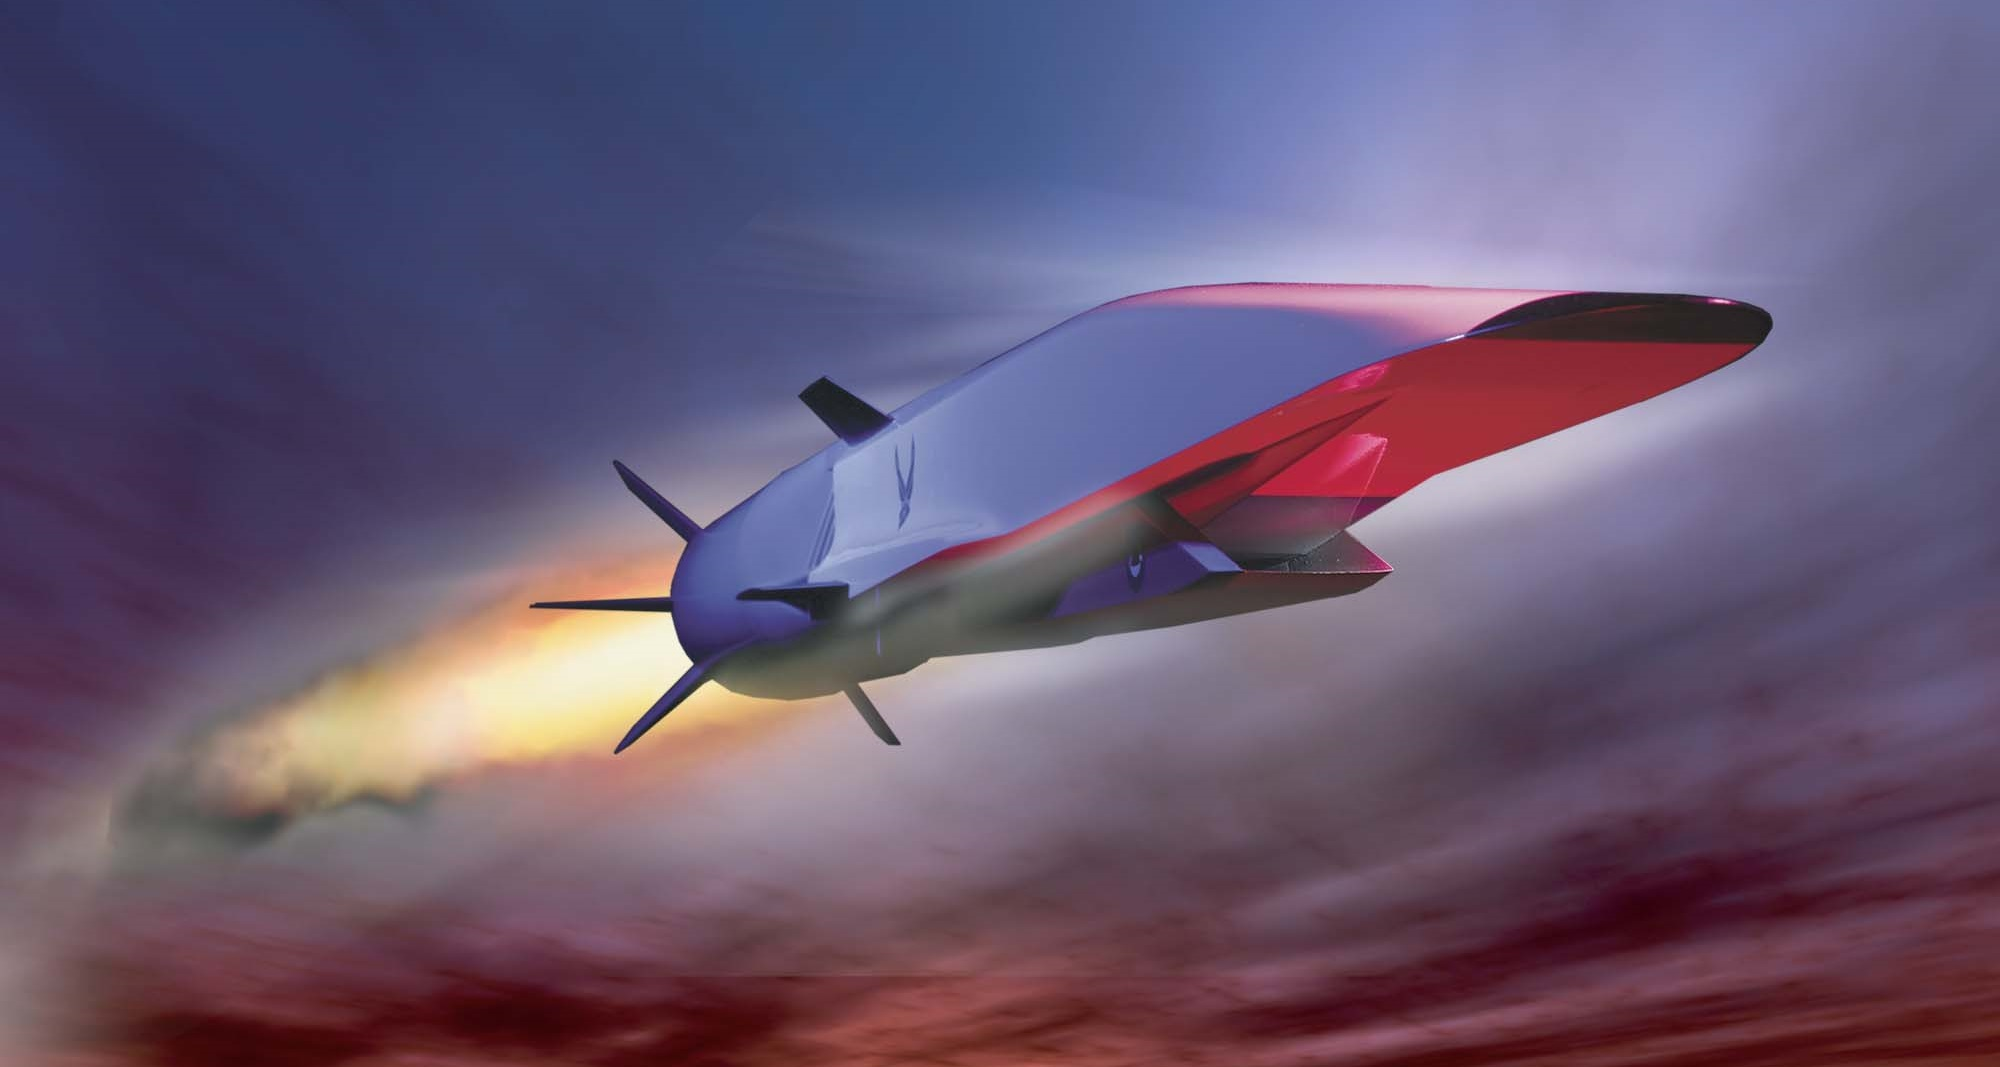
\includegraphics[width=3.5in]{\figurepath/boeing_x51_v3.jpg}
    \caption{Boeing X-51 waverider from Ref.\ \cite{x51picture}.}
  \end{center}
\end{figure}

The history of hypersonic flight is still in the making, with current research centered around the sustained flight of air-breathing vehicles.
The previous trajectories flown by aircraft such as the X-15, X-43 and X-51 were fairly benign in that abrupt and sudden maneuvers were generally avoided, and the goal was to demonstrate primarily the ability of these experimental aircraft to maintain hypersonic flight under their own power.
As technology grows the demands of these vehicles will grow too.
Current research is being performed to develop new materials and engine designs for these vehicles, as well as advanced control systems which will allow complex maneuvers to be performed while maintaining stability even in situations where unstart conditions are encountered.
One project in particular is the HIFiRE program, which is a collaboration between the U.S. Air Force Research Laboratory and the Defence Science Technology Organisation in Australia.
In particular, the HIFiRE 6 flight vehicle shown in Figure~\ref{fig.hifire6vehicle} is designed to evaluate the tracking performance of an adaptive flight control system on a representative hypersonic vehicle that is executing a set of predefined maneuvers\ \cite{adamczak.hifire6.2015, bolender.hifire6.2012, dauby.hifire6overview.2015}.

\begin{figure}[H]
  \begin{center}
    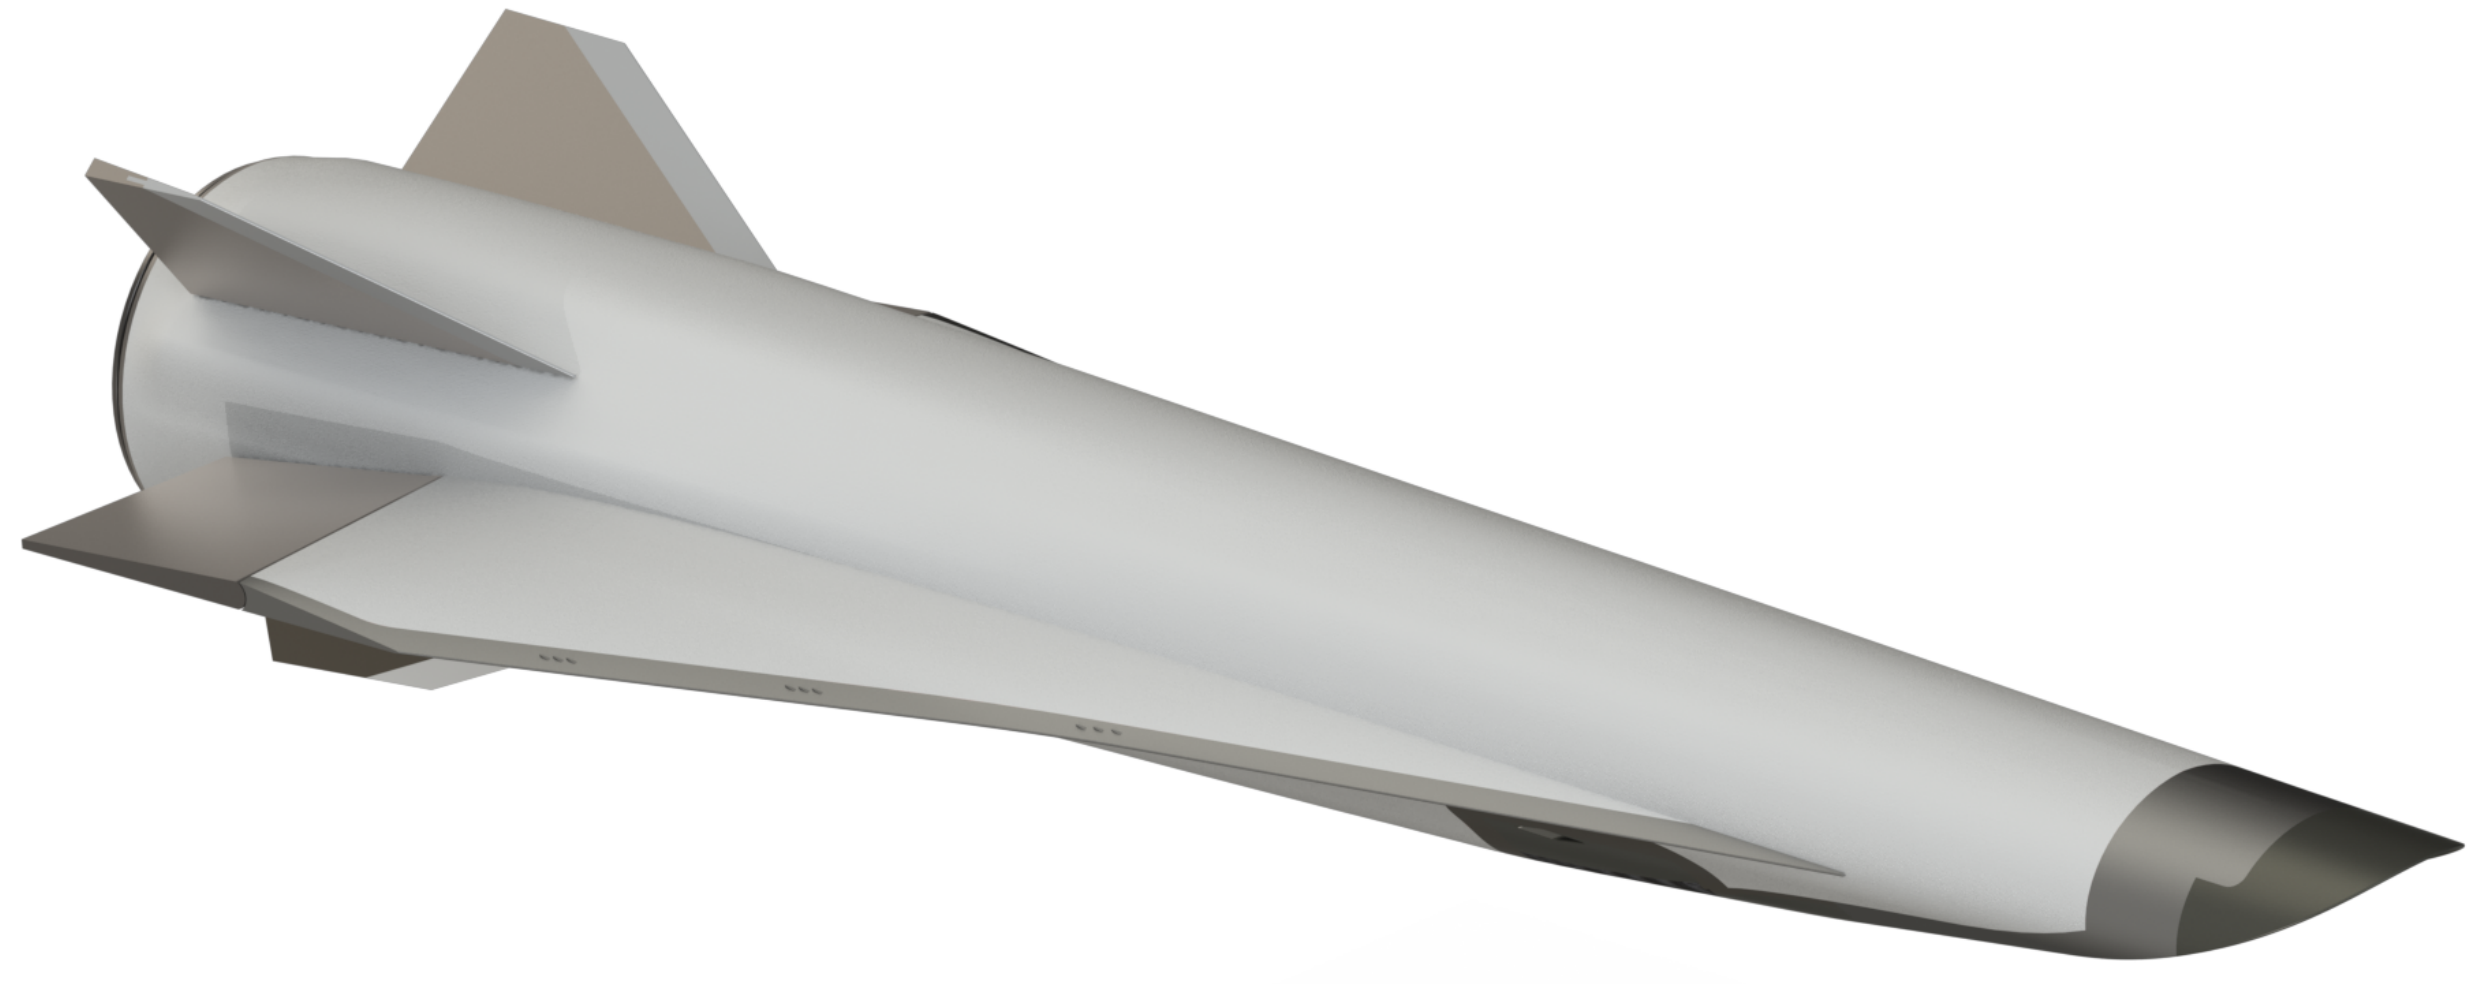
\includegraphics[width=3.5in]{\figurepath/hifire6.png}
    \caption{HIFiRE 6 flight vehicle from Ref.\ \cite{dauby.hifire6overview.2015}.\label{fig.hifire6vehicle}}
  \end{center}
\end{figure}

\subsection{Control of Hypersonic Vehicles}

The equations of motion which describe an aircraft are nonlinear, but in most cases it is acceptable to linearize these equations to facilitate control design and analysis.
This led to the description of aircraft dynamics using the transfer function, and to simple stability augmentation systems such as roll and yaw dampers\ \cite{cook.flightdynamics.2007}.
These flight control systems were simple, low-order, linear dynamic feedback compensators such as lead-lag and PID, and typically used small feedback gains\ \cite{dazzo.linearcontrol.2003, mclean.flightcontrol.1990, yechout.flightmechanics.2003}.
Thorough frequency domain analysis was critical to ensure a robust design.
Optimal control techniques slowly began seeing use in flight control in the early 1980s with limited success, but have now become more widely used\ \cite{abzug.stability.2005, chandler.lqrshortcomings.1983, stengel.flightdynamics.2004, stevenslewis.aircraftcontrol.2003}.
Many robust, nonlinear, and adaptive control solutions are proposed in recent literature\ \cite{bolender.hifire6.2012, gibson.adaptive.2008, huang.robust.2012, hughes.hinfinity.2010,   rollins.nonlinear.2013, xu.adaptive.2004} which include sliding mode, H$_{2}$/H$_{\infty}$, dynamic inversion, and neural network control, as well as many other techniques.

\section{Hypersonic Vehicle Modeling}

The Generic Hypersonic Vehicle (GHV) which is used as a platform for analysis and control design is shown in Figure~\ref{fig.ghvclouds}.
The GHV is a small, pilotless, blended wing-body vehicle, with 3-D inlet and nozzle, and axisymmetric through-flow scramjet engine.
There are four aerodynamic control surfaces which can be moved independently, consisting of two elevons and two rudders.
The relevant vehicle properties are listed in Table~\ref{tab:vehicle_properties}.

\begin{figure}[h]
  \begin{center}
    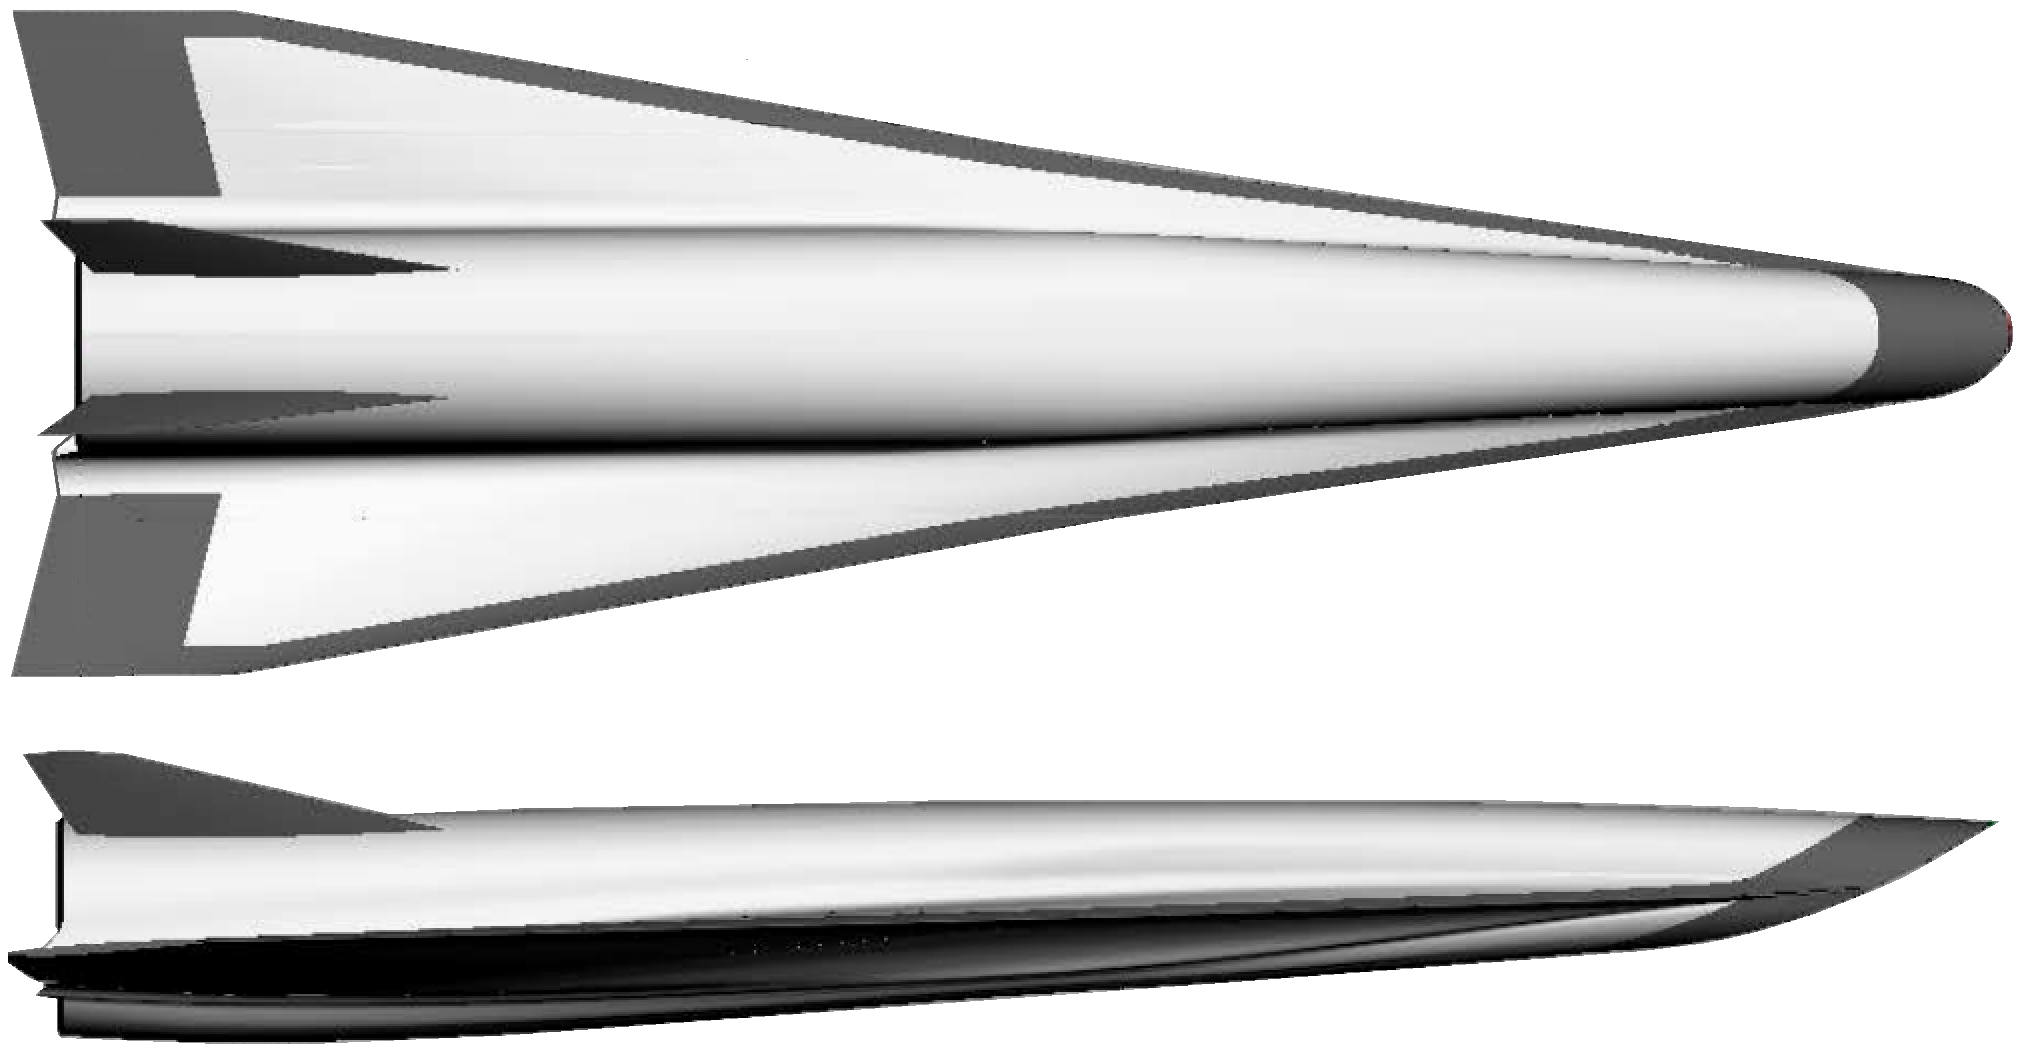
\includegraphics[width=4.5in]{\figurepath/ghvmodelview4.png}
    \caption{AFRL Generic Hypersonic Vehicle from Ref.\ \cite{ruttle.ghv.2012}.\label{fig.ghvclouds}}
  \end{center}
\end{figure}

The GHV was developed by the Air Force Research Lab in an effort to create a publicly releasable hypersonic vehicle model for studies of operability, controllability, and aero-propulsion integration as described in Reference\ \cite{ruttle.ghv.2012}.
The objective was to design a common vehicle which would be relevant to the technical efforts of current hypersonic projects, including the HIFiRE 6 vehicle, which the GHV closely resembles, as can be seen in Reference\ \cite{bolender.hifire6.2012}.
This GHV was designed be launched on rocket to accelerate to cruise at Mach 6, at a dynamic pressure of between 1000--2000 lb/ft$^{2}$.
The mission profile for the GHV then required maneuvers to be performed during the middle of the cruise phase before descending and decelerating, and making an unpowered maneuver to evaluate the potential to make a controlled landing.
The GHV has the capability to perform sustained maneuvers up to a load factor of up to approximately 2G.

\begin{table}[H]
  \centering
  \caption{Vehicle properties}
  \begin{tabular}{llr}
    \toprule
    Parameter & Unit & Value \\ \midrule
    Gross weight & [lbm] & $1220.3$ \\
    Empty weight & [lbm] & $993.3$ \\
    Vehicle length & [in] & $175.9$ \\
    Span & [in] & $58.6$ \\
    Nose diameter & [in] & $11.0$ \\
    Tail diameter & [in] & $18.8$ \\
    \bottomrule
  \end{tabular}\label{tab:vehicle_properties}
\end{table}

The aerodynamic data for the GHV was calculated using Hypersonic Engineering Aerothermodynamic Trajectory Tool Kit (HEAT-TK), developed for the Air Force by Boeing\ \cite{carter.heattk.2005}, and the engine data is calculated using the Ramjet Performance Analysis (RJPA) code, developed at Johns Hopkins University's Applied Physics Lab.

The equations of motion describing many aircraft can be derived assuming a flat, non-rotating Earth.
Due to the high flight speed of a hypersonic vehicle in the atmosphere, the rotation and curvature of the Earth are typically significant, and should not be neglected.
Thus, the governing equations of motion for the GHV are derived assuming the vehicle is a rigid body flying through the atmosphere of a spherical, rotating Earth.
The equations of motion describing the GHV are given in References\ \cite{billamoria.eom.1995, etkin.atmosphericflight.1972}, and will be presented in this chapter for completeness.

\subsubsection{Notation}
In deriving and applying the equations of motion which govern the motion of an aircraft, care must be taken to carefully book-keep the various vector quantities which describe the position, velocity and orientation of the aircraft.
For instance, when considering the velocity of an aircraft, it must be kept clear both with which frame the velocity is with respect to, and in which frame the velocity vector is described.
Some of the standard notation describing the expression of vectors in various reference frames is outlined below.
\begin{itemize}
  \item{$f_{a}$ denotes reference frame $a$.}
  \item{$O_{a}$ denotes the origin of reference frame $a$.}
  \item{$V^{a}_{b}$ describes the velocity of the origin of reference frame $b$ relative to the axes of reference frame $a$, described using the coordinate system of reference frame $b$.}
  \item{$\omega^{a,b}_{c}$ describes the angular velocity of reference frame $a$ relative to reference frame $b$ described using the axes of reference frame $c$. Omission of the second superscript implies the angular velocity of coordinate system $a$ is with respect to inertial axes. When the subscript is omitted, it is implied this quantity is described in the coordinates of frame $a$. For example $\omega^{B}$ is the inertial angular velocity of frame $f_{B}$, described using the axes of frame $f_{B}$.}
  \item{The transformation $R_{ab}$ describes a vector transformation from being expressed in reference frame $b$ to being expressed in reference frame $a$.}
  \item{$\frac{dV_{a}}{dt}\bigr|_{b}$ denotes the rate of change of $V_{a}$ with respect to frame $b$.}
  \item{All vectors are describing a relation of frame $a$ to frame $b$ are described along the axes of frame $a$.}
\end{itemize}

In many cases, the equations of motion can be greatly simplified when studying the dynamics of an aircraft.
Such simplifications often center around assuming the Earth is flat, but this may be an oversimplification for problems of hypersonic atmospheric flight.
While this simplification still might be acceptable for calculations involving the attitude dynamics where the rotating earth terms are typically very small, in trajectory calculations the rotating earth terms for a hypersonic vehicle become non-negligible.
This section presents the equations of motion that describe the GHV.\@

\subsection{Equations of Motion}

The equations of motion are developed using an Earth-centered, Earth-frame $f_{EC}$ with origin at the center of a spherical, rotating Earth.
It is assumed that the atmosphere travels uniformly with Earth as it rotates with angular velocity $\omega_{\text{earth}}$ in inertial space, and that the aircraft is sufficiently rigid that flexible structural effects can be neglected.
The position of the GHV around Earth and relative to $f_{EC}$ is described by its latitude $\lambda$, longitude $\tau$, and distance from the center of the Earth, $\mathscr{R}$.
These three coordinates give the location of the vehicle-carried frame $f_{V}$, defined with $z$-axis always pointing toward the origin of $f_{EC}$.

\begin{figure}[H]
  \begin{center}
    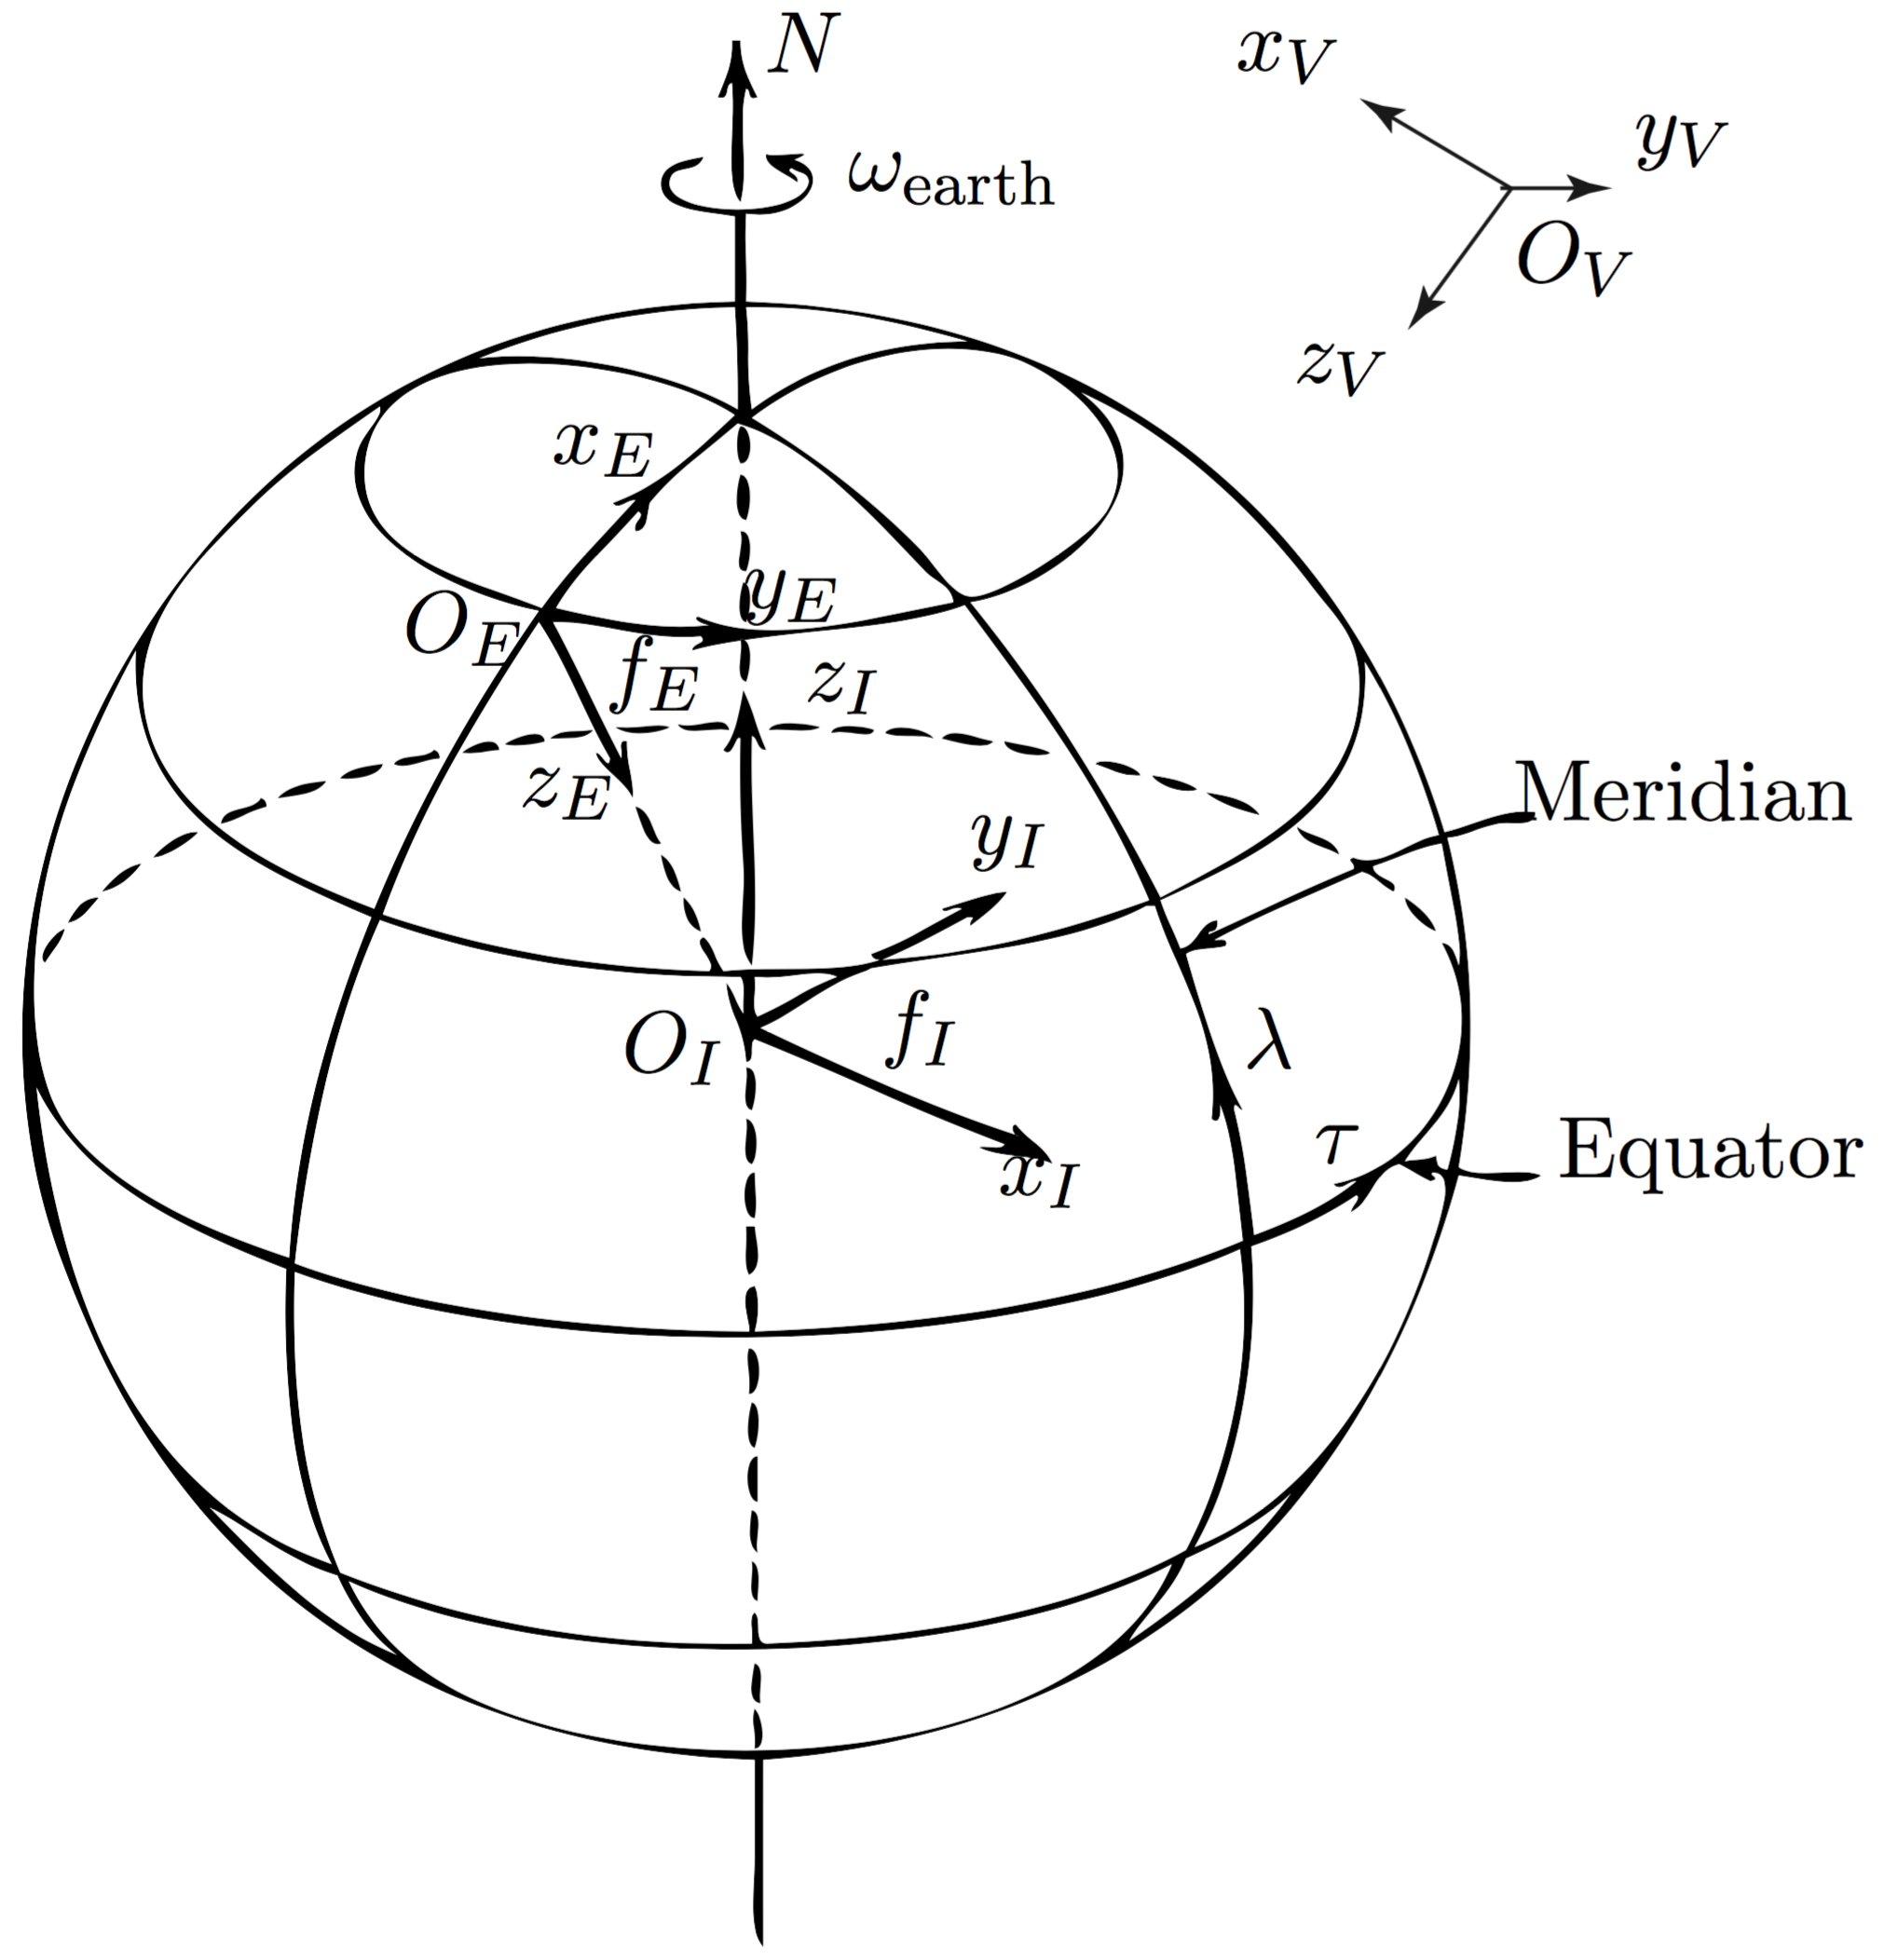
\includegraphics[height=2.5in]{\figurepath/globe_fig.png}
    \caption{Reference frames\ \cite{etkin.atmosphericflight.1972}\label{globe_fig}}
  \end{center}
\end{figure}

The vehicle carrying frame $f_{V}$ is a frame with origin attached to vehicle at the CG, and the z-axis $O_{V}z_{V}$ is defined to point vertically downward along the local $g$ vector.
$O_{V}x_{V}$ is defined to point north, and $O_{V}y_{V}$ east as shown in Figure~\ref{globe_fig}.
The vehicle-carried frame has angular velocity $\omega^{V}$ due to the curvature of the earth.
The body-fixed reference frame $f_{B}$ is a right-handed coordinate system attached to the GHV with $x$-axis pointing towards the nose of the aircraft along the longitudinal axis, and the $z$-axis pointing down.
This body-fixed axis system is used to derive the equations of motion for the GHV.\@

In deriving the equations of motion, the only additional assumption is that the centripetal acceleration due to $\omega_{\text{earth}}$ is negligible.
The equations of motion describe the dynamics of the GHV around the Earth when subject to external forces and moments.
These forces and moments, given in the body axes by $F_{B}$, and $M_{B}$ respectively, are due to the thrust and aerodynamic forces acting on the GHV, and are taken from pre-determined look-up tables within the simulation.
The aerodynamic forces depend on on control surface deflection angle, dynamic pressure, angle of attack, and sideslip angle.
The thrust forces depend on on control surface deflection angle, dynamic pressure, and angle of attack.

\subsubsection{Force Equations}

The force equation describing the the motion of the GHV center of gravity in body axes is given as the following
\begin{equation}
  \label{eqn.forceEqn}
  \frac{dV^{A}_{B}}{dt}\biggr|_{B}+\omega^{B}\times V^{A}_{B}+
  \omega^{E}_{B}\times V^{A}_{B}+\omega^{E}_{B}\times(\omega^{E}_{B}\times\mathscr{R})
  =
  g+(F_{A}+F_{T})/m
\end{equation}
where $V^{A}_{B}$ denotes the velocity of $f_{B}$ relative to the atmosphere-fixed reference frame, and $\omega^{E}_{B}$ is the inertial angular velocity of the Earth-fixed frame $f_{E}$, described using the coordinate system of the body reference frame.
Note in this work that the atmosphere is assumed fixed with respect to the earth, so $f_{A}=f_{E}$.
The components of the atmospheric velocity are
\begin{equation*}
  V_{B}^{A}=
  \bigr[
  \begin{array}{ccc}
    u & v & w
  \end{array}\bigr]^{\top}
\end{equation*}
The force vector $F_{B}$ that represents all non-gravitational forces acting on the body in body axes is given by
\begin{equation*}
  F_{B}=
  \bigr[
  \begin{array}{ccc}
    X & Y & Z
  \end{array}\bigr]^{\top}
\end{equation*}
In the Equation (\ref{eqn.forceEqn}) this force is separated into aerodynamic and propulsive contributions as $F_{B}=F_{A}+F_{T}$ where the aerodynamic and propulsive forces have components given by
\begin{equation}
  \label{eqn.AeroAndPropulsiveForces}
  \begin{split}
    F_{A}&=
    \bigr[
    \begin{array}{ccc}
      X_{A} & Y_{A} & Z_{A}
    \end{array}\bigr]^{\top} \\
    F_{T}&=
    \bigr[
    \begin{array}{ccc}
      X_{T} & Y_{T} & Z_{T}
    \end{array}\bigr]^{\top}
  \end{split}
\end{equation}

\subsubsection{Moment equations}

The vehicle moments are described by the following equation.
Note the absence of any rotor contributions to the vehicle moment, as the scramjet engine lacks moving parts, unlike jet-turbine powered craft.
\begin{equation}
  \label{eqn.momentEqn}
  J\frac{d\omega^{B}}{dt}\biggr|_{B}+\omega^{B}\times J\omega^{B}=M_{A}+M_{T}
\end{equation}
$\omega_{B}$ is the angular velocity of the body frame relative to the inertial frame, with the rate of change evaluated in the body frame, and components
\begin{equation*}
  \omega^{B}=
  \bigr[
  \begin{array}{ccc}
    p & q & r
  \end{array}\bigr]^{\top}
\end{equation*}
The total torque in body axes is given by
\begin{equation*}
  M_{B}=
  \bigr[
  \begin{array}{ccc}
    L & M & N
  \end{array}\bigr]^{\top}
\end{equation*}
This total moment is split into the contributions due to aerodynamic and propulsive moments in Equation (\ref{eqn.momentEqn}) as $M_{B}=M_{A}+M_{T}$ where the aerodynamic and propulsive moments have components given by
\begin{equation}
  \label{eqn.AeroAndPropulsiveMoments}
  \begin{split}
    M_{A}&=
    \bigr[
    \begin{array}{ccc}
      L_{A} & M_{A} & N_{A}
    \end{array}\bigr]^{\top} \\
    M_{T}&=
    \bigr[
    \begin{array}{ccc}
      L_{T} & M_{T} & N_{T}
    \end{array}\bigr]^{\top}
  \end{split}
\end{equation}
The moment of inertia matrix $J$ is given by
\begin{equation*}
  J=
  \begin{bmatrix}
    J_{xx} & -J_{xy} & -J_{xz} \\
    -J_{xy} & J_{yy} & -J_{yz} \\
    -J_{xz} & -J_{yz} & J_{zz}
  \end{bmatrix}
\end{equation*}
Without any simplification, expansion of the moment equations would become very cumbersome.
In general, aircraft are symmetric about the $x-z$ plane, mass is uniformly distributed, and the body coordinate system is oriented such that $J_{xy}=J_{yz}=0$.
This allows the moment of inertia matrix for the GHV to be simplified to
\begin{equation*}
  J=
  \begin{bmatrix}
    J_{xx} & 0 & -J_{xz} \\
    0 & J_{yy} & 0 \\
    -J_{xz} & 0 & J_{zz}
  \end{bmatrix}
\end{equation*}

\subsubsection{Orientation Equations}

The orientation, or kinematic equations describe the orientation of the aircraft body axes with respect to the vehicle carried frame.
The relationship between Euler rates and body angular velocities in the vehicle- carried frame is given by

\begin{equation}
  \label{eqn.bodyRatesToEulerRates}
  \left[
  \begin{array}{c}
    \dot{\phi} \\
    \dot{\theta} \\
    \dot{\psi}
  \end{array}\right]=
  \left[
  \begin{array}{ccc}
    1 & \tan(\theta)\sin(\phi) & \tan(\theta)\cos(\phi) \\
    0 & \cos(\phi) & -\sin(\phi) \\
    0 & \sin(\phi)/\cos(\theta) & \cos(\phi)/\cos(\theta)
  \end{array}\right]
  \left[
  \begin{array}{c}
    p_{v} \\
    q_{v} \\
    r_{v}
  \end{array}\right]
\end{equation}
where $\phi$, $\theta$, and $\psi$ are the roll, pitch, and yaw or heading angles, respectively, and are known as the Euer angles.
The components of angular velocities $p_{v}$, $q_{v}$, and $r_{v}$ are for the aircraft with body-fixed reference frame $f_{B}$ and are relative to the vehicle-carrying frame $f_{V}$.
These components of angular velocity are about the $x$, $y$, and $z$ body axes, respectively.
The relative angular velocities of the GHV are related to the vehicle absolute angular velocities by
\begin{equation*}
  \begin{bmatrix}
    p_{v} \\
    q_{v} \\
    r_{v}
  \end{bmatrix}=
  \begin{bmatrix}
    p \\
    q \\
    r
  \end{bmatrix}-R_{BV}
  \begin{bmatrix}
    (\omega_{\text{earth}}+\dot{\tau})\cos{\lambda} \\
    -\dot{\lambda} \\
    -(\omega_{\text{earth}}+\dot{\tau})\sin{\lambda}
  \end{bmatrix}
\end{equation*}
where $R_{BV}$ is the orthogonal rotation matrix given by
\begin{equation*}
  R_{BV}=
  \begin{bmatrix}
    \cos{\theta}\cos{\psi} & \cos{\theta}\sin{\psi} & -\sin{\theta} \\
    \sin{\phi}\sin{\theta}\cos{\psi}-\cos{\phi}\sin{\psi} &  \sin{\phi}\sin{\theta}\sin{\psi}+\cos{\phi}\cos{\psi} & \sin{\phi}\cos{\theta}\\
    \cos{\phi}\sin{\theta}\cos{\psi}+\sin{\phi}\sin{\psi} &  \cos{\phi}\sin{\theta}\sin{\psi}-\sin{\phi}\cos{\psi} & \cos{\phi}\cos{\theta}
  \end{bmatrix}
\end{equation*}

The reason for the distinction between relative and absolute angular rates in the above equations is due to the spherical Earth.
If a hypersonic vehicle was flying continuous circles around the world, the relative angular rates $p_{v}$, $q_{v}$, and $r_{v}$ would all be zero as the aircraft would be stationary relative to the vehicle carried frame.
However, the absolute angular rates $p$, $q$, and $r$ would be non-zero, as the vehicle carried frame would be rotating as it moved over the surface of the Earth.

\subsubsection{Navigation Equations}

The location, or navigation equations describe the location of the origin of the body fixed coordinate system with respect to the inertial axes.
The quantities describing this location are latitude, longitude, and altitude.
The navigation kinematic equation is given by
\begin{equation}
  \label{eqn.NavigationEqn}
  \begin{bmatrix}
    \dot{\lambda}\mathscr{R} \\
    \dot{\tau}\mathscr{R}\cos{\lambda} \\
    -\dot{\mathscr{R}}
  \end{bmatrix}=R_{VB}
  \begin{bmatrix}
    u \\
    v \\
    w
  \end{bmatrix}
\end{equation}
where $R_{VB}=R_{BV}^{-1}$.

\subsection{State Space Representation}

The aerodynamic and propulsive forces and moments in\ \eqref{eqn.AeroAndPropulsiveForces} and\ \eqref{eqn.AeroAndPropulsiveMoments}, respectively depend on the vehicle state and input.
With this, the equations of motion in\ \eqref{eqn.forceEqn},\ \eqref{eqn.momentEqn},\ \eqref{eqn.bodyRatesToEulerRates}, and\ \eqref{eqn.NavigationEqn} can be represented in state-space form as
\begin{equation}
  \label{eqn.nonlinearStateSpace}
  \dot{X}(t) = f\bigr({X}(t), U(t)\bigr)
\end{equation}
with state vector
\begin{equation}
  \label{eqn.fullstatevectorx}
  X=\left[
  \begin{array}{cccccccccccc}
    V_{T} &  \alpha & q &\theta & h & \beta &p & r & \phi &\psi &\lambda & \tau
  \end{array}\right]^{\top}
\end{equation}
where $V_{T}$ is the total velocity, $\alpha$ and $\beta$ are the angle of attack and sideslip angle, $\phi$, $\theta$, and $\psi$ are the roll, pitch, and yaw angles, $p$, $q$, and $r$ are the absolute angular velocity components, and $\lambda$, $\tau$, and $h$ are the latitude, longitude, and altitude, of the GHV, respectively.
The input vector is given by
\begin{equation}
  \label{eqn.fullcontrolvector}
  U=\left[
  \begin{array}{cccc}
    u_{\text{th}} & u_{\text{elv}} & u_{\text{ail}} & u_{\text{rud}}
  \end{array}\right]^{\top}
\end{equation}
where $u_{\text{th}}$, $u_{\text{elv}}$, $u_{\text{ail}}$, and $u_{\text{rud}}$ are the throttle, elevator, aileron, and rudder inputs, respectively.
The entries of the state vector are arranged so as to facilitate separation of the lateral and longitudinal equations of motion during control design.
The deflection of the elevons are accomplished through static mixing, combining differential and collective deflections from the aileron and elevator commands, respectively, while both rudders are actuated together using the single rudder input.
The control vector $U_{5}$ contains the deflections of the right and left elevons ($u_{r,\text{elv}}$, $u_{l,\text{elv}}$), rudders ($u_{r,\text{rud}}$, $u_{l,\text{rud}}$), and throttle as
\begin{equation*}
  U_{5}=
  \bigr[
  \begin{array}{ccccc}
    u_{\text{th}} & u_{r,\text{elv}} & u_{l,\text{elv}} & u_{r,\text{rud}}  & u_{l,\text{rud}}
  \end{array}\bigr]^{\top}
\end{equation*}
The control allocation matrix $M$ is the matrix which defines the following transformation between control vectors $U_{5}$ and $U$ as
\begin{equation*}
  U = MU_{5}
\end{equation*}
where control allocation matrix is
\begin{equation*}
  M=
  \left[
  \begin{array}{ccccc}
    1 & 0 & 0 & 0 & 0 \\
    0 & 1/2 & 1/2 & 0 & 0 \\
    0 & 1/2 & -1/2 & 0 & 0 \\
    0 & 0 & 0 & 1/2 & 1/2 \\
  \end{array}\right]
\end{equation*}


\section{Open-Loop Analysis}

The open-loop behavior of the GHV was analyzed about a nominal flight condition of $M=6$, $h=80,000$ ft, corresponding to a dynamic pressure of 1,474 lb/ft$^2$.
The geographical coordinates and heading of the GHV are insignificant in the equations of motion for the purposes of inner-loop control law development, and these state variables are dropped from the state vector (\ref{eqn.fullstatevectorx}) for trim, linearization, and control.
\begin{equation}
  \label{eqn.truncstatevectorx}
  X=\bigr[
  \begin{array}{ccccccccc}
    V_{T} &  \alpha & q &\theta & h & \beta &p & r & \phi
  \end{array}\bigr]^{\top}
\end{equation}
The state $X$ from this point forward is used to mean the truncated state (\ref{eqn.truncstatevectorx}), as it contains the primary quantities describing the vehicle dynamics that are to be controlled.

\subsection{Linearization}

The dynamics of the system with truncated state are described by\ \eqref{eqn.nonlinearStateSpace}.
The equilibrium, or trim state $X_{\text{eq}}$ and input $U_{\text{eq}}$ satisfy
\begin{equation}
  \label{eqn.eqptdef}
  \dot{X}_{\text{eq}}=f({X}_{\text{eq}},U_{\text{eq}})=0
\end{equation}
The equilibrium state and input are found for the nominal steady, level cruise condition, and Equation (\ref{eqn.nonlinearStateSpace}) is linearized about this trim condition as follows.
Defining $x$ and $u$ to be state and input perturbations about equilibrium, the state and input can be expressed as
\begin{equation*}
  \begin{split}
    X(t) &= X_{\text{eq}} + x(t) \\
    U(t) &= U_{\text{eq}} + u(t)
  \end{split}
\end{equation*}
Differentiating (\ref{eqn.nonlinearStateSpace})
\begin{equation}
  \label{eqn.Xdotxdotfxu}
  \begin{split}
    \dot{X}(t) = \dot{x}(t)
    &= f\bigr(X(t), U(t)\bigr) \\
    &= f\bigr(X_{\text{eq}}+x(t),U_{\text{eq}}+u(t)\bigr)
  \end{split}
\end{equation}
Performing a Taylor series expansion, neglecting second order terms and higher
\begin{equation}
  \label{eqn.TaylorSeriesExpansionNonlinearEqn}
  \dot{x}= f(X_{\text{eq}},U_{\text{eq}})+\left.\frac{\partial f(X,U)}{\partial X}\right|_{\text{eq}}x+\left.\frac{\partial f(X,U)}{\partial U}\right|_{\text{eq}}u+\epsilon
\end{equation}
where the subscript $(\cdot)_{\text{eq}}$ indicates these quantities be evaluated at the equilibrium point.
With $f(X_{\text{eq}},U_{\text{eq}})=0$, the linearization results in the state-space system given by
\begin{equation}
  \label{eqn.linearStateSpace}
  \dot{x}(t) = Ax(t) + Bu(t)
\end{equation}
where
\begin{equation*}
  A = \left.\frac{\partial f(X,U)}{\partial X}\right|_{\text{eq}}^{}
  \hspace{0.5in}
  B = \left.\frac{\partial f(X,U)}{\partial U}\right|_{\text{eq}}^{}
\end{equation*}
Using this linear system, the open-loop dynamic modes of the GHV during the nominal steady level cruise condition are analyzed through a sensitivity analysis.
It is also important to note that the perturbation state $x$ of the linear system in Equation (\ref{eqn.linearStateSpace}) will be represented as having the following components.
\begin{equation*}
  x=\bigr[
  \begin{array}{ccccccccc}
    \Delta V_{T} & \Delta\alpha & \Delta q & \Delta\theta & \Delta h & \Delta\beta & \Delta p & \Delta r & \Delta\phi
  \end{array}\bigr]^{\top}
\end{equation*}
The perturbation input for the linear system is equivalently defined as
\begin{equation*}
  u=\left[
  \begin{array}{cccc}
    \Delta\delta_{\text{th}} & \Delta\delta_{\text{elv}} & \Delta\delta_{\text{ail}} & \Delta\delta_{\text{rud}}
  \end{array}\right]^{\top}
\end{equation*}
In following sections, this notation is abused by not explicitly including the $\Delta$ preceding each component to indicate that the components of the state vector $x$ and input vector $u$ are in fact perturbation states and inputs, respectively.
This is done only when there is no possibility of confusion, and so when referring to the state and control input of the linear system given by Equation (\ref{eqn.linearStateSpace}) the following notation will be used
\begin{equation}
  \label{eqn.perturbedstatevectorx}
  x=\bigr[
  \begin{array}{ccccccccc}
    V_{T} &  \alpha & q &\theta & h & \beta &p & r & \phi
  \end{array}\bigr]^{\top}
\end{equation}
\begin{equation}
  u=\left[
  \begin{array}{cccc}
    \delta_{\text{th}} & \delta_{\text{elv}} & \delta_{\text{ail}} & \delta_{\text{rud}}
  \end{array}\right]^{\top}
\end{equation}

\subsubsection{Linear Assumption}

The nonlinear equations of motion in\ \eqref{eqn.nonlinearStateSpace} were linearized resulting in\ \eqref{eqn.linearStateSpace} and analyzed.
In this section the validity of this linear assumption is examined.
In particular, it is desired to get a sense of the size of $\epsilon$ in\ \eqref{eqn.TaylorSeriesExpansionNonlinearEqn} as the perturbation terms $x$ and $u$ increasingly deviate the linearized system from the equilibrium point.

The nonlinear function in\ \eqref{eqn.Xdotxdotfxu} and its linear counterpart in\ \eqref{eqn.linearStateSpace} could be evaluated for different values of $x(t)$ and $u(t)$, and difference them to explicitly determine $\epsilon$.
However, since this system has dimension higher than two, and has entries which have many different units, it will be difficult to get a sense in this way, as to what the region looks like around the trim point where the aircraft can be operated and still reasonably satisfy the linear assumption.

An alternative, which is possible in the case of stable systems, is to look at the initial condition response of both the linear and nonlinear systems to get a sense of how the two differ.
However, because the hypersonic vehicle model used for this work is unstable, this approach is not possible.
For this reason, the response of the linear and nonlinear model were compared in simulation when using the closed-loop controller, to verify the validity of the linear assumption.

\subsection{Modal Analysis}

Given a linear system such as Equation (\ref{eqn.linearStateSpace}) it is often of interest to examine the system modes.
Conventional aircraft usually have modes which are quite predictable in their characteristics from one vehicle to the next, but with an aircraft such as the GHV, the significant state variables in the different modes may differ from those of conventional aircraft.
Because of this it is crucial to analyze the system modes to better understand the dynamics of the GHV in order to facilitate the control design process.

The sensitivity matrix for the linear system given in Equation (\ref{eqn.linearStateSpace}) is calculated, which contains the desired modal information.
The sensitivity analysis aims to determine which entries in a given eigenvector are small when the units of each state variable are not the same.
This method examines slight changes in the initial condition of each state separately in order to determine whether this change will influence some modes more strongly than others.
This analysis will provide knowledge of what modes the GHV exhibits, which states are dominant in each of these modes, as well as the stability of these modes.

\subsubsection*{Mode Sensitivity} %ref etkin pg66

Consider the linear system (\ref{eqn.linearStateSpace}) describing the GHV dynamics, with perturbation state vector given by (\ref{eqn.perturbedstatevectorx}).
This section outlines the method presented in\ \cite{etkin.atmosphericflight.1972} of applying a linear transformation to a state space system to obtain a system represented in characteristic coordinate system to facilitate the modal analysis and calculation of the sensitivity matrix.
Considering only the initial condition response, the following autonomous system results
\begin{equation}
  \label{eqn.xdotax}
  \dot{x}(t) = Ax(t)
\end{equation}
The following nonsingular transformation is introduced
\begin{equation*}
  x(t) = \mathbb{V}q(t)
\end{equation*}
where $\mathbb{V}\triangleq[\begin{array}{ccc} \mathrm{v}_{1} & \cdots & \mathrm{v}_{n} \end{array}]$ is the modal matrix made up of the eigenvectors or $A$ as shown.
Note that this transformation will not alter the eigenvalues or eigenvectors of the system in (\ref{eqn.xdotax}).
Using this transformation
\begin{equation*}
  \dot{q}(t) = \tilde{A}q(t)
\end{equation*}
where
\begin{equation*}
  \tilde{A}=\mathbb{V}^{-1}A\mathbb{V}
\end{equation*}
The matrix $\mathbb{V}^{-1}A\mathbb{V}$ can be expressed as
\begin{equation*}
  A\mathbb{V}
  =A \left[
  \begin{array}{ccc}
    \mathrm{v}_{1} & \cdots & \mathrm{v}_{n}
  \end{array} \right]
  =\left[
  \begin{array}{ccc}
    A\mathrm{v}_{1} & \cdots & A\mathrm{v}_{n}
  \end{array}\right]
  =\left[
  \begin{array}{ccc}
    \mathrm{v}_{1}\lambda_{1} & \cdots & \mathrm{v}_{n}\lambda_{n}
  \end{array}\right]
  =\mathbb{V}\Lambda%
\end{equation*}
giving
\begin{equation*}
  \dot{q}(t) =\Lambda q(t)
\end{equation*}
where $\Lambda$ is the diagonal matrix of eigenvalues.
The solution is given by
\begin{equation*}
  q(t)=e^{\Lambda t}q(0)
\end{equation*}
The unforced response of the system in response to initial conditions is of interest.
In particular, an initial condition is selected as a scalar multiple of an eigenvector $\mathrm{v}_{i}$
\begin{equation*}
  x(0)=\alpha_{i}\mathrm{v}_{i}
\end{equation*}
Using the linear transformation
\begin{equation*}
  \begin{split}
    q(0)
    &= \mathbb{V}^{-1}x(0) \\
    &= \alpha_{i}\mathbb{V}^{-1}\mathrm{v}_{i}
  \end{split}
\end{equation*}
Since $\mathbb{V}^{-1}\mathbb{V}=\mathbb{I}$ where $\mathbb{I}$ is the identity matrix, $\mathbb{V}^{-1}\mathrm{v}_{i}$ is just the $\mathrm{i^{th}}$ column of $\mathbb{I}$.
In other words, the initial condition $q(0)$ corresponding to the selected $x(0)$ will be a column vector of zeros, with the exception of the entry $\alpha_{i}$ in the $\mathrm{i^{th}}$ row.
The response of the state $x(t)$ from this initial condition is given by
\begin{equation*}
  \begin{split}
    x(t)&=\mathbb{V}e^{\Lambda{t}}\alpha_{i}\mathbb{V}^{-1}\mathrm{v}_{i} \\
    &=\alpha_{i}\mathbb{V}e^{\Lambda{t}}
    \bigr[
    \begin{array}{ccccc}
      0 & \hdots & 1 & \hdots & 0
    \end{array}\bigr]^{\top}
  \end{split}
\end{equation*}
Expanding
\begin{equation*}
  \begin{split}
    x(t)&=\alpha_{i}
    \left[
    \begin{array}{ccc}
      \mathrm{v}_{1} & \cdots & \mathrm{v}_{n}
    \end{array} \right]
    \left[
    \begin{array}{cccc}
      e^{\lambda_{1}t} & 0 & \cdots & 0 \\
      0 & e^{\lambda_{2}t} & \cdots & 0 \\
      \vdots & \vdots & \ddots & \vdots \\
      0 & 0 & \cdots & e^{\lambda_{n}t}
    \end{array}\right]
    \begin{bmatrix}
      0 \\
      \vdots \\
      1 \\
      \vdots \\
      0
    \end{bmatrix} \\
    &=\alpha_{i}e^{\lambda_{i}t}\mathrm{v}_{i}
  \end{split}
\end{equation*}
This shows that only the mode corresponding to $\lambda_{i}$ will be present in the response from an initial condition along the $\mathrm{i^{th}}$ eigenvector.
The general response in terms of $x$ is given by summing the individual responses starting from each eigenvector initial condition
\begin{equation*}
  x(t)=\sum \limits_{i=1}^{n} \alpha_{i}e^{\lambda_{i}t}\mathrm{v}_{i}
\end{equation*}
Based on this unforced modal response, if any entries in $\mathrm{v}_{i}$ are small relative to the others, the corresponding states are thus not influential in determining the initial condition response.

\subsubsection*{Calculating the Sensitivity Matrix}

In this section the methods of\ \cite{durham.flightdynamics.2013, manual.durham.2002} used to calculate the sensitivity matrix for $\tilde{A}$ are outlined.
The matrix $\mathbb{V}$ and its inverse $\mathbb{V}^{-1}$ are first calculated.
The rows of $\mathbb{V}$ are denoted using $r_{i}$, and the columns of $\mathbb{V}^{-1}$ as $c_{i}$
\begin{equation*}
  \mathbb{V}=
  \bigr[
  \begin{array}{cccc}
    r_{1}^{\top} & r_{2}^{\top} & \hdots & r_{n} ^{\top}
  \end{array}\bigr]^{\top}
  \hspace{0.5in}
  \mathbb{V}^{-1}=\left[
  \begin{array}{cccc}
    c_{1} & c_{2} & \cdots & c_{n}
  \end{array}\right]
\end{equation*}
The diagonal matrices $C_{i}$ are formed using the elements of $c_{i}$
\begin{equation*}
  c_{i}=\left[
  \begin{array}{c}
    c_{i,1} \\
    c_{i,2} \\
    \vdots \\
    c_{i,n}
  \end{array}\right] \hspace{0.5in}
  C_{i}=\left[
  \begin{array}{cccc}
    c_{i,1} & 0 & \cdots & 0 \\
    0 & c_{i,2} & \cdots & 0 \\
    \vdots & \vdots & \ddots & \vdots \\
    0 & 0 & \cdots & c_{i,n}
  \end{array}\right]
\end{equation*}
The $n \times n$ sensitivity matrix $S$ is defined as
\begin{equation*}
  S\equiv\left[
  \begin{array}{c}
    r_{1}C_{1} \\
    r_{2}C_{2} \\
    \vdots \\
    r_{n}C_{n}
  \end{array}\right]
\end{equation*}

\subsubsection*{Sensitivity Matrix Analysis: Nominal Flight Condition}

The sensitivity matrix $S$ is shown in Table~\ref{sensmat_fc1_1} for a nominal flight condition of flight Mach number $M=6$ and altitude $h=80,000$ ft, giving a dynamic pressure of $\bar{q}=1,474$ psf.

\begin{table}[H]
  \centering
  \caption{Sensitivity matrix: nominal flight condition}
  \fontsize{8pt}{8pt}\selectfont
  \begin{tabularx}{0.95\textwidth}{|X|XXXXX|XXXX|} % chktex 44
    \cline{2-10}
    \multicolumn{1}{c|}{} & $\lambda_{1}$ & $\lambda_{2}$ & $\lambda_{3}$ & $\lambda_{4}$ & $\lambda_{5}$ & $\lambda_{6}$ & $\lambda_{7}$ & $\lambda_{8}$ & $\lambda_{9}$ \\
    \multicolumn{1}{c|}{} &  -2.24 & -4.87 & 1.89 & \multicolumn{2}{c|}{$1.37\pm 0.76\mathrm{j}$} & \multicolumn{2}{c}{$0\pm 0.12\mathrm{j}$} & -0.0039 & -0.0272 \\
    \hline % chktex 44
    $V_{T}$ & 3.44E-05 & 1.22E-13 & 6.57E-05 & 1.34E-10 & 1.34E-10 & 0.0022 & 0.0022 & \textbf{0.9955} & 2.46E-09 \\ \hline % chktex 44
    $\alpha$ & \textbf{0.3618} & 7.31E-10 & \textbf{0.3226} & 3.04E-08 & 3.04E-08 & \textbf{0.1578} & \textbf{0.1578} & 3.04E-05 & 4.96E-10 \\
    $q$     & \textbf{0.4823} & 1.05E-09 & \textbf{0.5103} & 4.97E-08 & 4.97E-08 & 0.0036 & 0.0036 & 2.48E-07 & 4.57E-12 \\
    $\theta$ & 0.0088 & 1.79E-11 & 0.0160 & 3.92E-09 & 3.92E-09 & \textbf{0.4876} & \textbf{0.4876} & 5.32E-05 & 1.59E-09 \\
    $h$     & 0.0012 & 9.70E-13 & 0.0020 & 5.77E-10 & 5.77E-10 & \textbf{0.4962} & \textbf{0.4962} & 0.0044 & 8.55E-10 \\ \hline % chktex 44
    $\beta$ & 1.79E-10 & \textbf{0.2311} & 1.16E-07 & \textbf{0.3844} & \textbf{0.3844} & 3.17E-11 & 3.17E-11 & 3.30E-15 & 7.59E-05 \\
    $p$     & 2.81E-09 & \textbf{0.4259} & 5.66E-08 & \textbf{0.2855} & \textbf{0.2855} & 7.34E-10 & 7.34E-10 & 4.73E-12 & 0.0031 \\
    $r$     & 3.87E-10 & 0.0119 & 9.56E-09 & \textbf{0.3412} & \textbf{0.3412} & 7.91E-09 & 7.91E-09 & 1.73E-10 & \textbf{0.3058} \\
    $\phi$ & 5.01E-11 & 0.0237 & 4.84E-08 & \textbf{0.3096} & \textbf{0.3096} & 1.08E-08 & 1.08E-08 & 2.88E-09 & \textbf{0.3570} \\
    \lasthline%
  \end{tabularx}\label{sensmat_fc1_1}
\end{table}
Each row corresponds to a state, and the modes corresponding to the columns.
In each column, the magnitude of the each entry indicates how influential this corresponding state is in the mode corresponding to that column.
The values in any given column which are at least one order of magnitude greater than the other values are shown in bold, showing the states which are most dominant in each mode.
The smallest terms, which are several orders of magnitude less than the largest values in each mode do not significantly impact the response.
These values are removed, as shown in the sensitivity matrix in Table~\ref{sensmat_fc1_2}.
\begin{table}[H]
  \centering
  \caption{Sensitivity matrix: nominal flight condition}
  \fontsize{8pt}{8pt}\selectfont
  \begin{tabularx}{0.95\textwidth}{|X|XXXXX|XXXX|} % chktex 44
    \cline{2-10}
    \multicolumn{1}{c|}{} & $\lambda_{1}$     & $\lambda_{2}$     & $\lambda_{3}$     & $\lambda_{4}$     & $\lambda_{5}$    & $\lambda_{6}$     & $\lambda_{7}$     & $\lambda_{8}$     & $\lambda_{9}$ \\
    \multicolumn{1}{c|}{} &  -2.24 & -4.87 & 1.89 & \multicolumn{2}{c|}{$1.37\pm 0.76\mathrm{j}$} & \multicolumn{2}{c}{$0\pm 0.12\mathrm{j}$} & -0.0039 & -0.0272 \\
    \hline % chktex 44
    $V_{T}$ & \textemdash{} & \textemdash{} & \textemdash{} & \textemdash{} & \textemdash{} & 0.0022 & 0.0022 & \textbf{0.9955} & \textemdash{} \\ \hline % chktex 44
    $\alpha$ & \textbf{0.3618} & \textemdash{} & \textbf{0.3226} & \textemdash{} & \textemdash{} & \textbf{0.1578} & \textbf{0.1578} & \textemdash{} & \textemdash{} \\
    $q$     & \textbf{0.4823} & \textemdash{} & \textbf{0.5103} & \textemdash{} & \textemdash{} & 0.0036 & 0.0036 & \textemdash{} & \textemdash{} \\
    $\theta$ & 0.0088 & \textemdash{} & 0.0160 & \textemdash{} & \textemdash{} & \textbf{0.4876} & \textbf{0.4876} & \textemdash{} & \textemdash{} \\
    $h$     & 0.0012 & \textemdash{} & 0.0020 & \textemdash{} & \textemdash{} & \textbf{0.4962} & \textbf{0.4962} & 0.0044 & \textemdash{} \\ \hline % chktex 44
    $\beta$ & \textemdash{} & \textbf{0.2311} & \textemdash{} & \textbf{0.3844} & \textbf{0.3844} & \textemdash{} & \textemdash{} & \textemdash{} & \textemdash{} \\
    $p$     & \textemdash{} & \textbf{0.4259} & \textemdash{} & \textbf{0.2855} & \textbf{0.2855} & \textemdash{} & \textemdash{} & \textemdash{} & 0.0031 \\
    $r$     & \textemdash{} & 0.0119 & \textemdash{} & \textbf{0.3412} & \textbf{0.3412} & \textemdash{} & \textemdash{} & \textemdash{} & \textbf{0.3058} \\
    $\phi$ & \textemdash{} & 0.0237 & \textemdash{} & \textbf{0.3096} & \textbf{0.3096} & \textemdash{} & \textemdash{} & \textemdash{} & \textbf{0.3570} \\
    \lasthline%
  \end{tabularx}\label{sensmat_fc1_2}
\end{table}

Table~\ref{sensmat_fc1_2} shows the influence of the significant states on each mode.
From this, it can be seen that the assumption of decoupled lateral and longitudinal dynamics is a good one.
None of the lateral states are present in any of the longitudinal modes, and none of the longitudinal states are present in the lateral modes.
Comparing the magnitude of the entries in the sensitivity matrix for the GHV, each of the modes was separated by at least one order of magnitude difference, indicating a strong decoupling of the flight modes.

\subsubsection{Summary of Flight Modes}

The sensitivity analysis indicated the presence of two longitudinal and three lateral flight modes as shown in Figure~\ref{fig:poleplot}.
The GHV has a highly unstable irregular short period mode and an unstable dutch roll mode.
The phugoid mode is neutrally stable, and the rolling mode is stable.
The velocity mode is given by a pole at the origin, and is omitted from Figure~\ref{fig:poleplot}.

\begin{figure}[H]
  \centering
  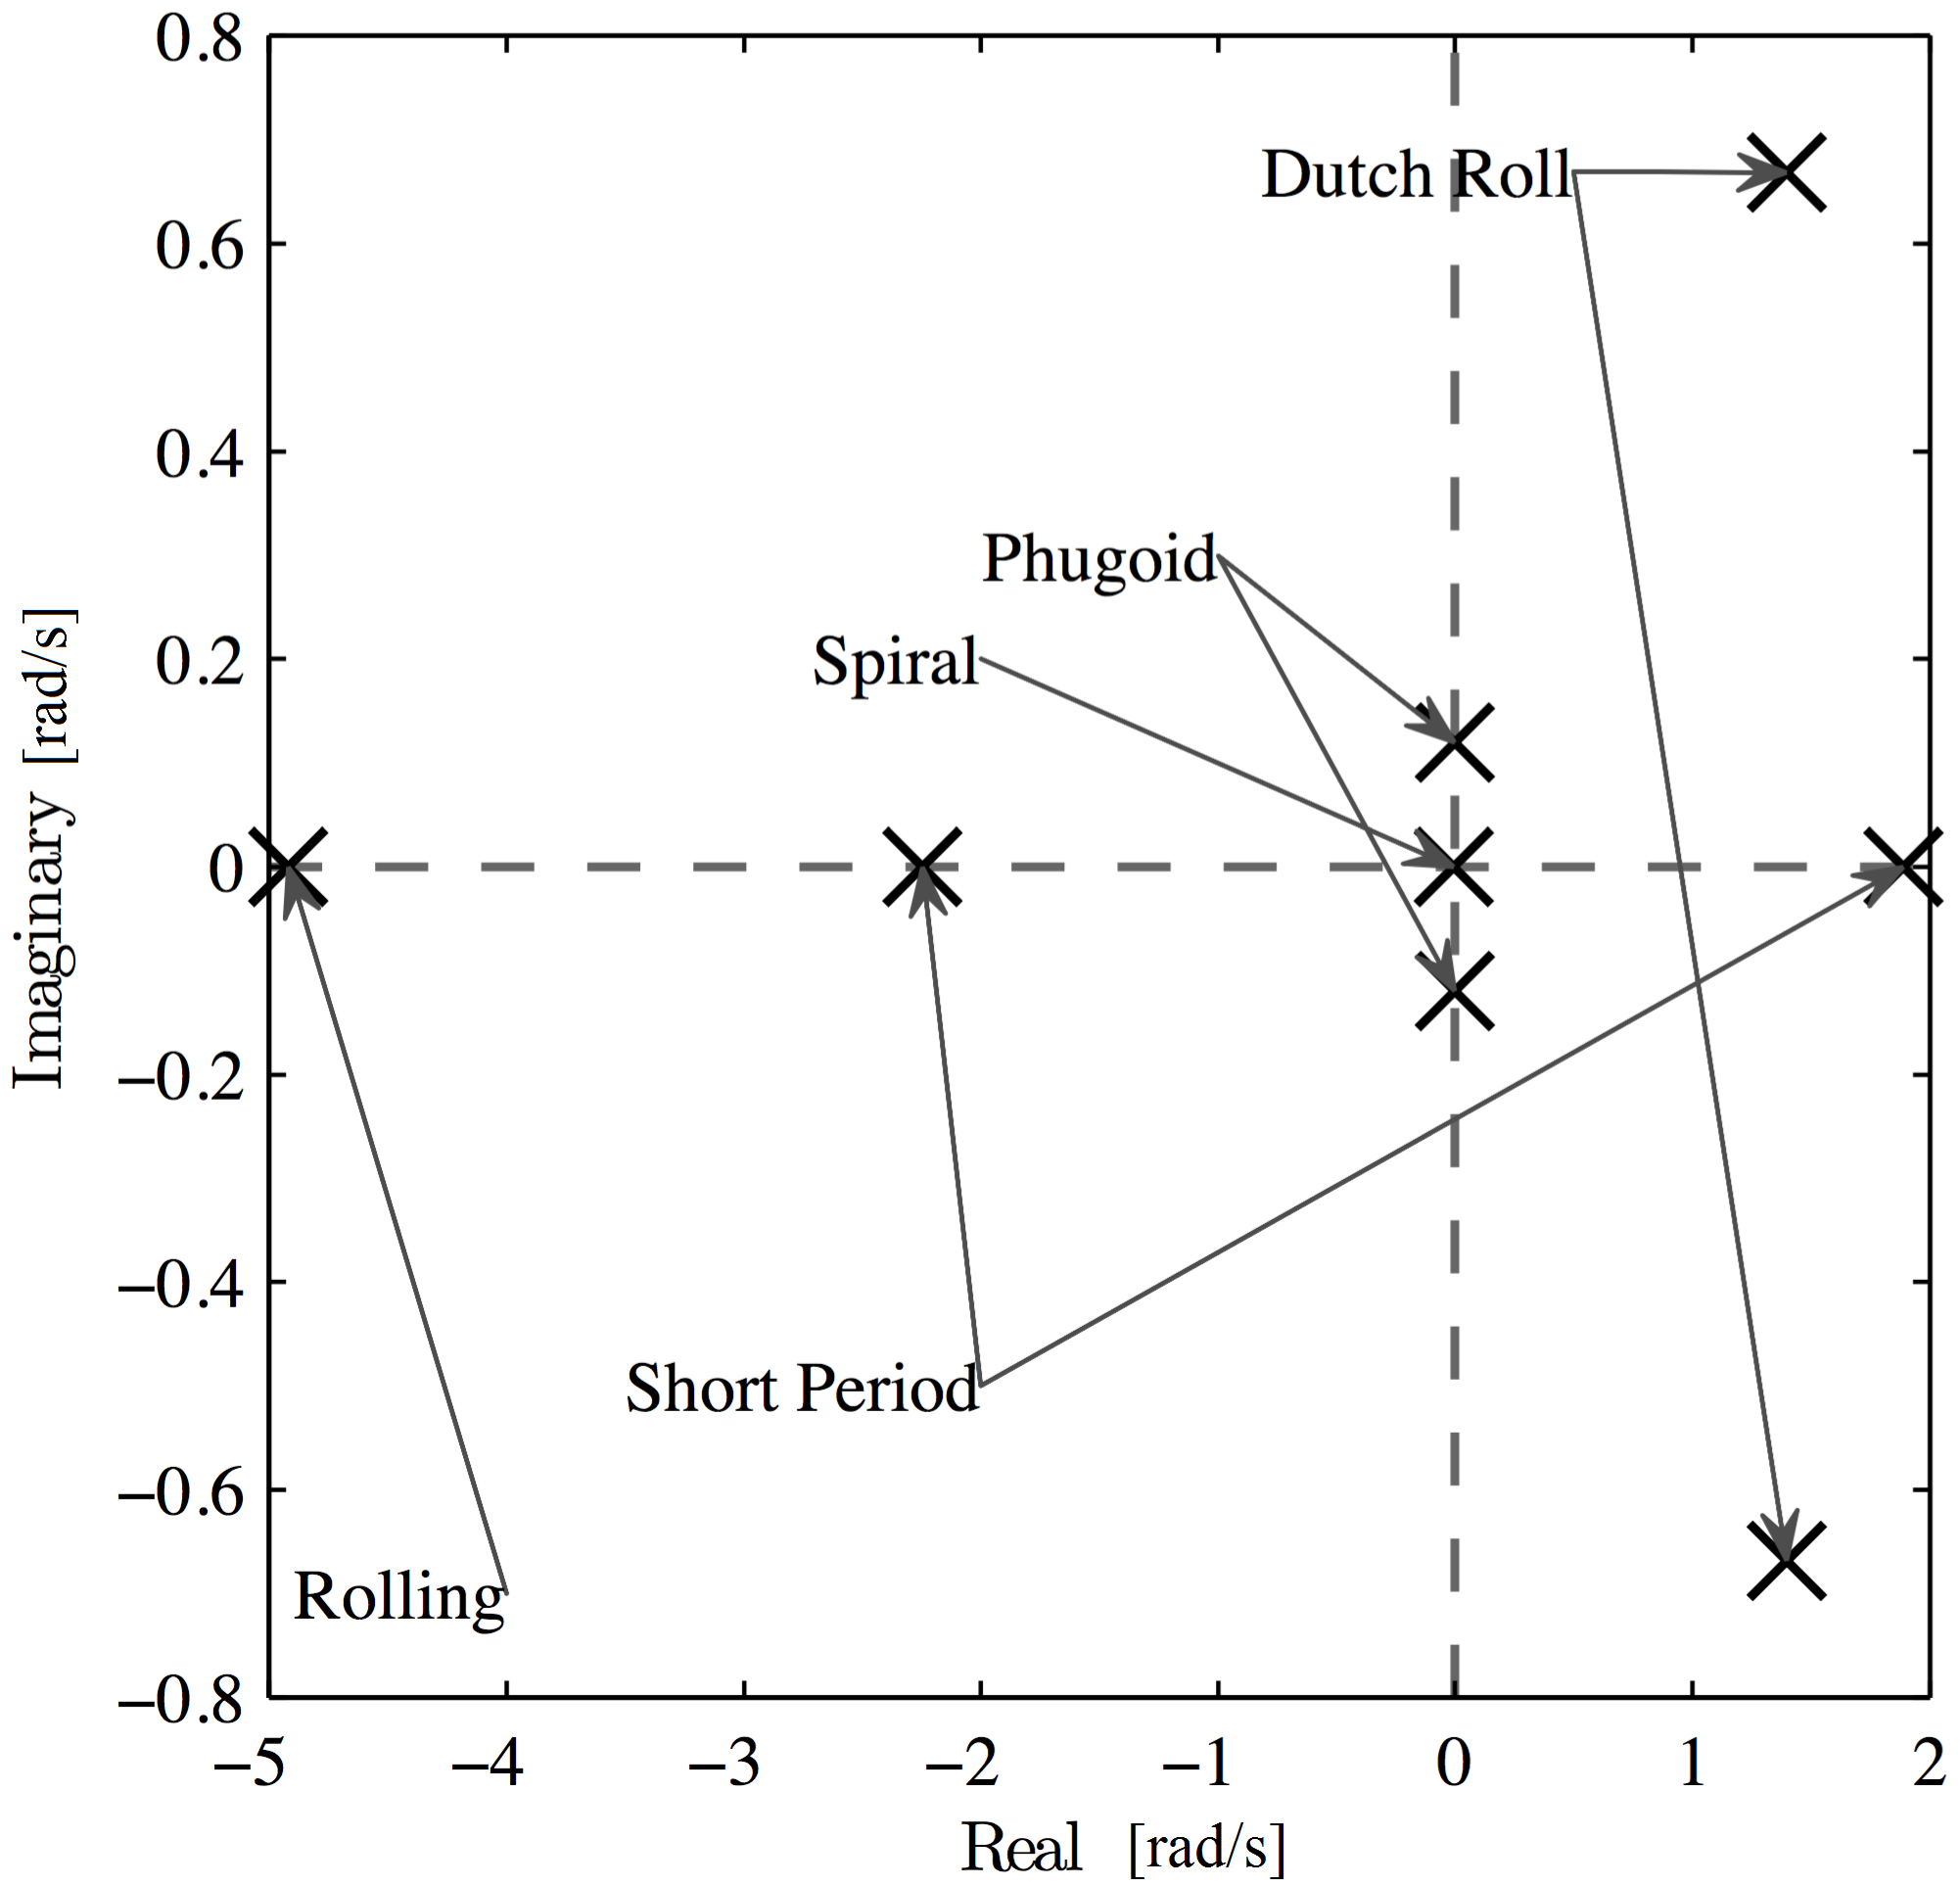
\includegraphics[width=4.0in]{\figurepath/openLoopPoles.png}
  \caption{Open-loop poles of $A$ for $M=6$, $h=80,000$ ft steady, level cruise\label{fig:poleplot}}
\end{figure}

The sensitivity analysis performed above indicates the presence of six flight modes.
These modes are explained below.
\begin{itemize}\itemsep2pt
  \item{\textbf{Short Period} ($\lambda_{1,3}$) \textemdash{} an unstable mode dominated by $\alpha$ and $q$. Relatively fast, purely real poles, with $\lambda_{1,3}\approx\pm2$.}
  \item{\textbf{Rolling} ($\lambda_{2}$) \textemdash{} a stable mode, dominated by $\beta$ and $p$. Fast, real pole at $\lambda_{2}=-4.9$.}
  \item{\textbf{Dutch-Roll} ($\lambda_{4,5}$) \textemdash{} an unstable mode, which is a combination of a rolling, pitching, and yawing motion in flight.}
  \item{\textbf{Phugoid} ($\lambda_{6,7}$) \textemdash{} a neutrally stable phugoid-type mode.}
  \item{\textbf{Velocity} ($\lambda_{8}$) \textemdash{} neutrally stable.}
  \item{\textbf{Spiral} ($\lambda_{9}$) \textemdash{} a slow, but stable mode.}
\end{itemize}
The eigenvalues corresponding to the different modes are shown in the pole plot in Figure~\ref{fig:poleplot}.
The pole corresponding to the velocity mode is dropped, since it has no affect on any of the other longitudinal dynamics.
This stability analysis was repeated at several other flight conditions, and revealed the same basic modes, although the pole locations and stability of some of the modes differed from the flight condition shown here.

\section{Model for Control Design}

The above sections presented the nonlinear equations of motion which describe the dynamics of the GHV, linearized these equations, and then analyzed them to determine the validity of the linearization, and decouple the linear system into several reduced order systems: the velocity, longitudinal, and lateral-directional subsystems.
The modal analysis showed the decoupling of the velocity, longitudinal, and lateral modes, allowing each of these three subsystems to be considered independently.
This allows the control design of the GHV to be simplified, by having to design three lower order controllers, as opposed to a single higher order controller.
The velocity and longitudinal subsystems are both single input systems.
The throttle input $u_{\text{th}}$ controls only the velocity $V_{T}$, and the elevator input $u_{\text{elv}}$ controls the longitudinal states.
The lateral subsystem is multi input, with the aileron $u_{\text{ail}}$ and tail $u_{\text{rud}}$ as control inputs.
Before the control design for each of the three subsystems is presented, a few paragraphs are devoted to providing some additional background on the types of uncertainty that are present in the hypersonic vehicle and as in\ \eqref{eqn.wholeSystemUncertain}, and that are studied in the simulation results presented in this chapter.

\subsection{Model Uncertainty}

A model is only a mathematical representation of a system or process, and so the presence of uncertainty in any plant model is inevitable.
This is particularly true in the case of a hypersonic vehicles, due in part to engine/airframe coupling, complex shock interactions, flexible effects, and unsteady aerodynamics\ \cite{mcruer.hypersonic.1991,schmidt.dynamics.1992,rudd.hypersonic.2010}.
When building a more conventional vehicle such as a subsonic transport aircraft, much wind tunnel and flight test data is collected, and the aerodynamic coefficients describing the aircraft can in general be determined with a high level of accuracy\ \cite{maine.coefficients.1981,morelli.parameters.1997}.
This data is difficult to obtain for a hypersonic vehicle, where wind tunnel testing is more difficult to do.
Additionally an extremely limited amount of hypersonic flight test data has ever been recorded, especially for air-breathing hypersonic vehicles.
Existing analytical techniques often fail to accurately predict the stability derivatives for air-breathing vehicles due to hypersonic flow assumptions which are violated due to the presence of the engine\ \cite{rudd.integrated.2000}.
The use of CFD has become increasingly used to model the aerodynamics of hypersonic vehicles, but there is still much work to be done.
Because of these challenges, uncertainties in the values of the aerodynamic properties, such as in the stability derivatives of up to several hundred percent, are possible in a hypersonic vehicle.

Additionally, loss in control effectiveness can occur through damage sustained during flight, as depicted in Figure~\ref{fig:flapdamage}, degradation over time, as well as for similar reasons as above: the aerodynamic forces and moments generated by a control surface deflection are different from those forces and moments as predicted through modeling.

\begin{figure}[H]
  \begin{center}
    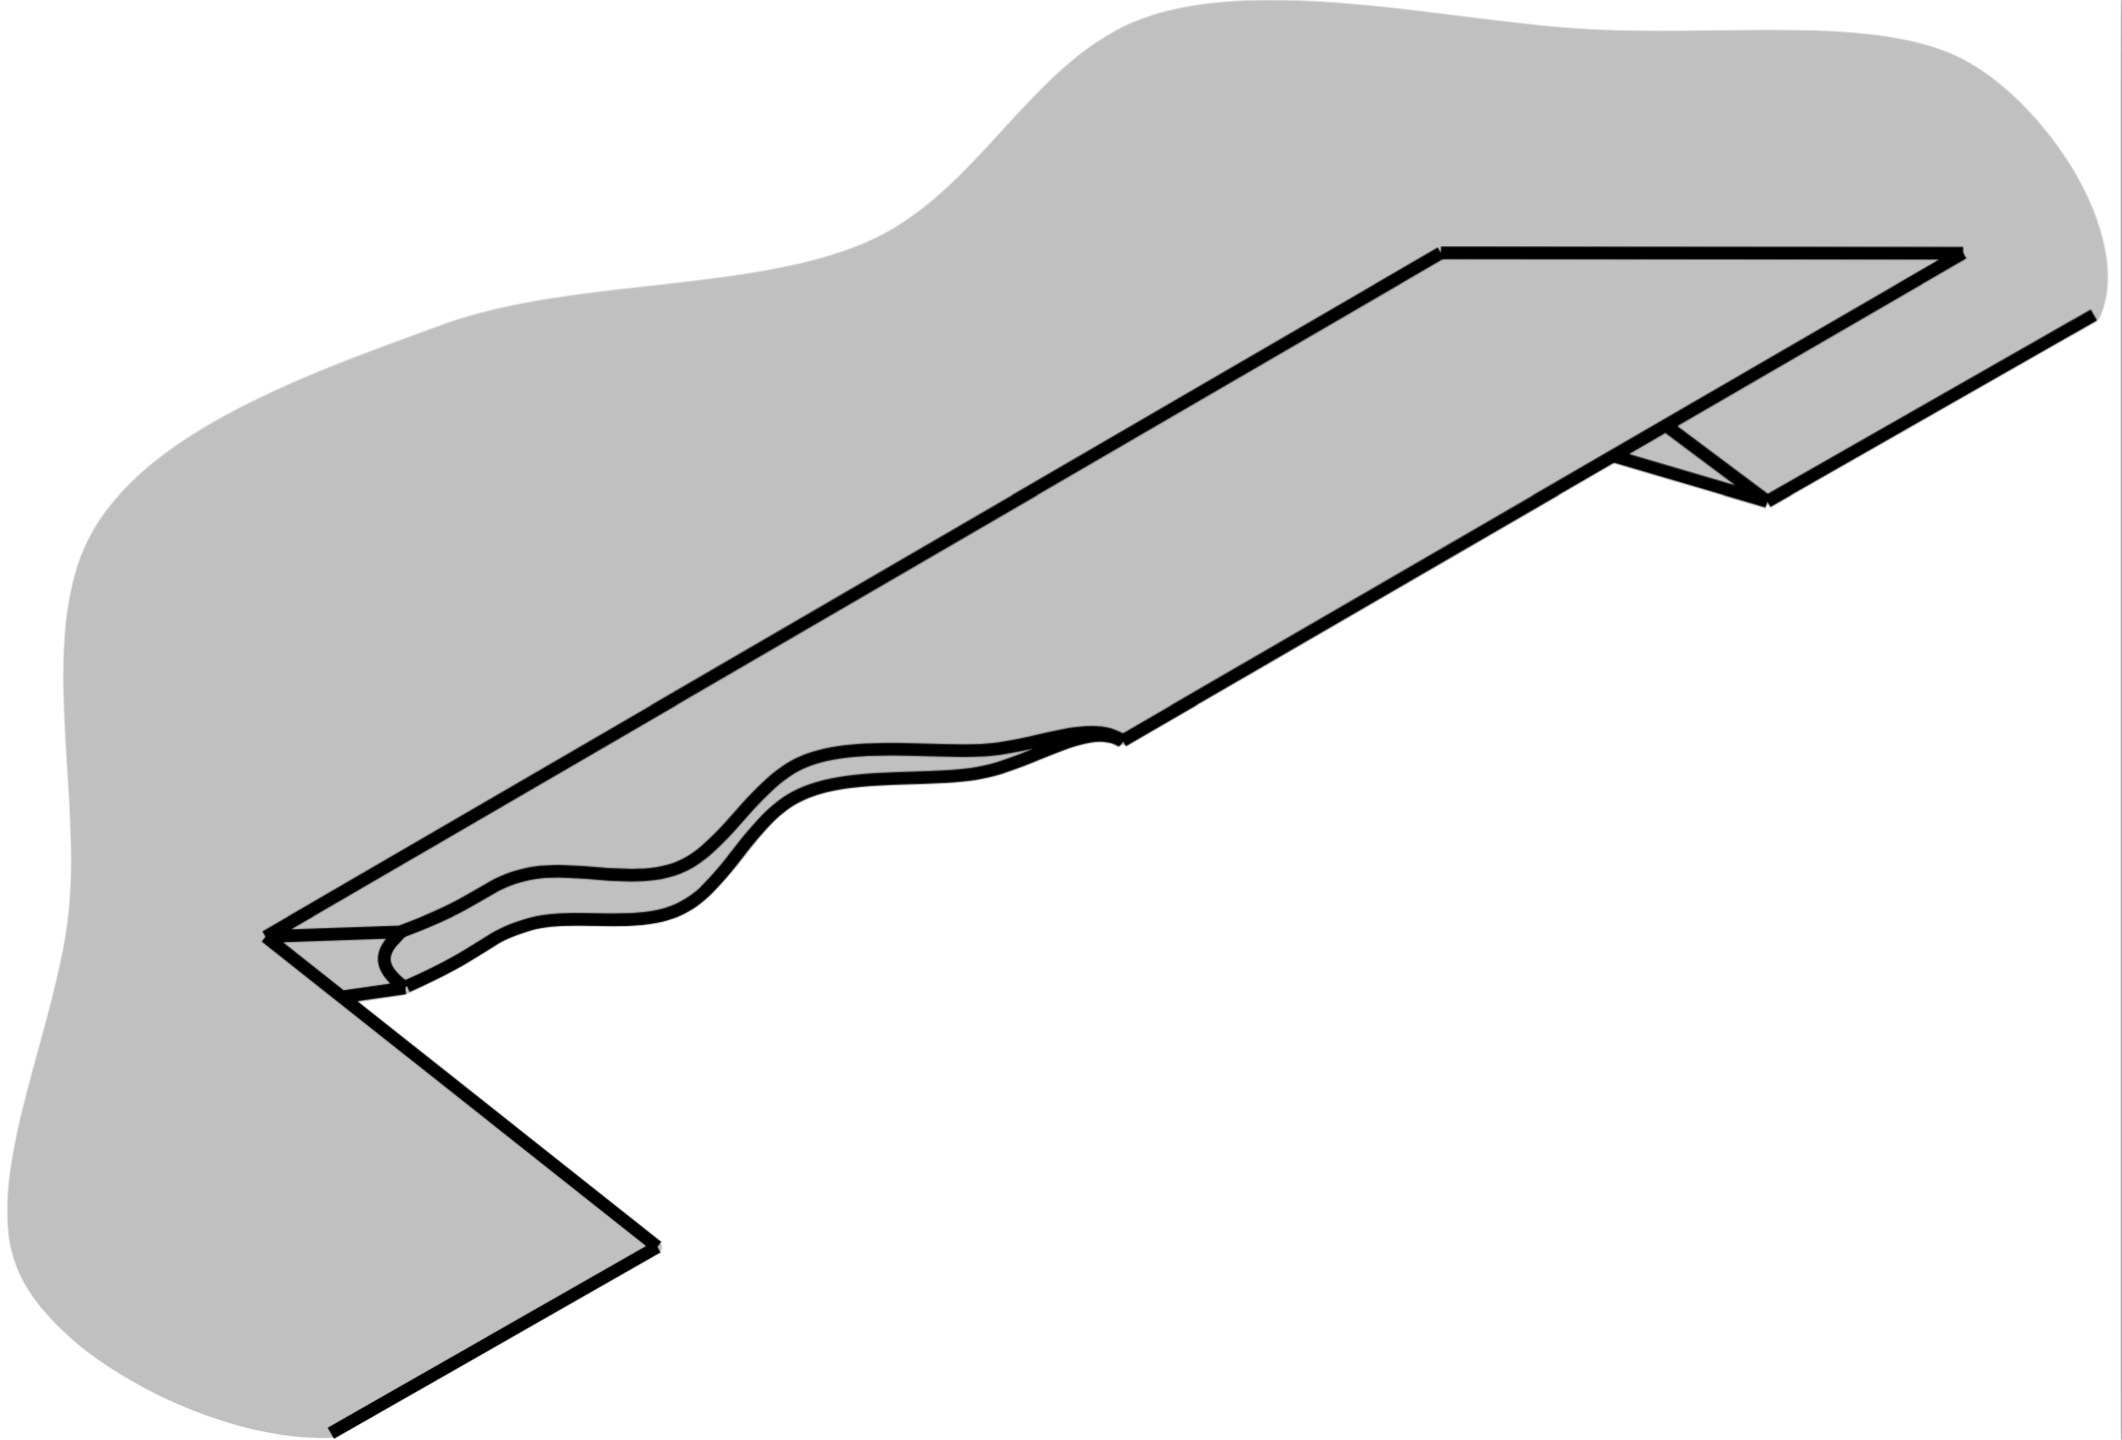
\includegraphics[width=2.0in]{\figurepath/flap2.png}
    \caption{Uncertainty in control effectiveness due to control surface damage\label{fig:flapdamage}}
  \end{center}
\end{figure}

Conventional aircraft can typically have significant variations in the center of gravity location.
These variations are minimized by careful loading of the aircraft, and by placing fuel tanks as close as is practicable to the center of gravity location so as to minimize the CG shift due to fuel burn.
The GHV will not be carrying any auxiliary payload, and it is the goal to have fuel tanks which are as close to the CG as possible.
Even so, uncertainty in the center of gravity location is inevitable and can greatly impact the stability of the vehicle.
Furthermore, changes in center-of-gravity location have a similar effect on the stability of the vehicle as shifts and uncertainty in the center-of-pressure location.
Thus, assuming uncertainty in center-of-gravity location also captures the effect of uncertainty in the center-of-pressure, which is very common in hypersonic vehicles.

\subsection{The Three Control Subsystems}

The three subsystems that the plant was separated into based on the distinct flight modes allowed for the design of multiple lower order controllers.
Each of the subsystems of the plant for which a controller will be designed is outlined here.

\subsubsection{Velocity Subsystem}

From the sensitivity analysis, the total velocity is decoupled from the rest of the states, allowing a separate controller to be designed to regulate and control only velocity.
The perturbation state, input, measured output, and regulated output used in the design of the velocity controller are given by
\begin{equation*}
  x_{p} = V_{T}
  \qquad
  u = \delta_{\text{th}}
  \qquad
  y_{p} = V_{T}
  \qquad
  z_{p} = V_{T}
\end{equation*}
For the velocity subsystem $n_{p}=1$ and $m=1$, and is a state-feedback problem.
Integral action is applied for tracking velocity reference commands.
That is $n_{ep}=1$.
The state-space matrices for the velocity subsystem represented by\ \eqref{eqn.xdotpunc} are given by
\begin{equation*}
  A_{p} = X_{v}
  \qquad
  B_{p} = X_{u_{\text{th}}}\cos(\alpha_{\text{eq}})
  \qquad
  C_{p} = 1
  \qquad
  C_{pz} = 1
  \qquad
  D_{pz} = 0
\end{equation*}

\subsubsection{Longitudinal Subsystem}

The uncertain, linear, longitudinal dynamics of the GHV in the form of\eqref{eqn.wholeSystemUncertain} are described as follows\ \cite{stengel.flightdynamics.2004}.
\begin{equation*}
  \begin{bmatrix}
    \dot{\alpha} \\
    \dot{q} \\
    \dot{\theta} \\
    \dot{h}
  \end{bmatrix}=
  \begin{bmatrix}
    \frac{Z_{\alpha}}{v_{\text{eq}}-Z_{\dot{\alpha}}} & \frac{v_{\text{eq}}+Z_{q}}{v_{\text{eq}}-Z_{\dot{\alpha}}} & -\frac{g\sin{\gamma_{\text{eq}}}}{v_{\text{eq}}-Z_{\dot{\alpha}}} & 0 \\
    M_{\alpha}+\frac{M_{\dot{\alpha}}Z_{\alpha}}{v_{\text{eq}}-Z_{\dot{\alpha}}} & M_{q}+\frac{M_{\dot{\alpha}}(v_{\text{eq}}+Z_{q})}{v_{\text{eq}}-Z_{\dot{\alpha}}} & M_{\theta}-\frac{M_{\dot{\alpha}}g\sin(\gamma_{\text{eq}})}{v_{\text{eq}}-Z_{\dot{\alpha}}} & 0 \\
    0 & 1 & 0 & 0 \\
    -v_{\text{eq}}\cos(\gamma_{\text{eq}}) & 0 & v_{\text{eq}}\cos(\gamma_{\text{eq}}) & 0 \\
  \end{bmatrix}
  \begin{bmatrix}
    \alpha \\
    q \\
    \theta \\
    h
  \end{bmatrix}+
  \begin{bmatrix}
    \frac{Z_{u_{\text{elv}}}}{v_{\text{eq}}-Z_{\dot{\alpha}}} \\
    M_{u_{\text{elv}}}+\frac{M_{\dot{\alpha}}Z_{u_{\text{elv}}}}{v_{\text{eq}}-Z_{\dot{\alpha}}} \\
    0 \\
    0
  \end{bmatrix}
  u_{\text{elv}}
\end{equation*}

\paragraph{Inner-loop}
Partitioning the longitudinal dynamics gives the inner-loop short-period dynamics as described by\ \eqref{eqn.innerLoopDynamicsUncertain} with plant matrices given by
\begin{equation*}
  \begin{gathered}
    A_{p} =
    \begin{bmatrix}
      \frac{Z_{\alpha}}{v_{\text{eq}}-Z_{\dot{\alpha}}} & \frac{v_{\text{eq}}+Z_{q}}{v_{\text{eq}}-Z_{\dot{\alpha}}} \\
      M_{\alpha}+\frac{M_{\dot{\alpha}}Z_{\alpha}}{v_{\text{eq}}-Z_{\dot{\alpha}}} & M_{q}+\frac{M_{\dot{\alpha}}(v_{\text{eq}}+Z_{q})}{v_{\text{eq}}-Z_{\dot{\alpha}}} \\
    \end{bmatrix}
    \qquad
    B_{p} =
    \begin{bmatrix}
      \frac{Z_{u_{\text{elv}}}}{v_{\text{eq}}-Z_{\dot{\alpha}}} \\
      M_{u_{\text{elv}}}+\frac{M_{\dot{\alpha}}Z_{u_{\text{elv}}}}{v_{\text{eq}}-Z_{\dot{\alpha}}} \\
    \end{bmatrix} \\[8pt]
    B_{gd} =
      \begin{bmatrix}
      -\frac{g\sin{\gamma_{\text{eq}}}}{v_{\text{eq}}-Z_{\dot{\alpha}}} & 0 \\
      M_{\theta}-\frac{M_{\dot{\alpha}}g\sin(\gamma_{\text{eq}})}{v_{\text{eq}}-Z_{\dot{\alpha}}} & 0 \\
    \end{bmatrix}
    \qquad
    C_{p} =
    \begin{bmatrix}
      0 \\
      1
    \end{bmatrix}^{\top}
    \qquad
    C_{pz} =
    \begin{bmatrix}
      0 \\
      1
    \end{bmatrix}^{\top}
  \end{gathered}
\end{equation*}
and with $D_{pz} = 0$.
To design the inner-loop controller for the longitudinal subsystem, the $B_{gd}$ term in\ \eqref{eqn.innerLoopDynamicsUncertain} for the inner-loop short-period dynamics is neglected, giving a system in the form of\ \eqref{eqn.xdotpunc} where the state, control, measured output, and regulated output for the inner-loop linear longitudinal subsystem are given by
\begin{equation*}
  x_{p} =
  \begin{bmatrix}
    \alpha & q
  \end{bmatrix}^{\top}
  \hspace{0.5in}
  u = \delta_{e}
  \hspace{0.5in}
  y_{p} = q
  \hspace{0.5in}
  z_{p} = q
\end{equation*}
The pitch rate is measurable but the angle of attack is not.
The inner-loop control goal is to track pitch rate commands $z_{p,\text{cmd}}=q_{\text{cmd}}$.

\paragraph{Outer-loop}
The plant matrices for the outer-loop phugoid dynamics in the form of\ \eqref{eqn.outerLoopDynamics} are given by
\begin{equation*}
  \begin{gathered}
    A_{g} =
    \begin{bmatrix}
      0 & 0 \\
      v_{\text{eq}}\cos(\gamma_{\text{eq}}) & 0
    \end{bmatrix}
    \qquad
    B_{pg} =
    \begin{bmatrix}
      0 & 1 \\
      -v_{\text{eq}}\cos(\gamma_{\text{eq}}) & 0 \\
    \end{bmatrix}
    \qquad
    C_{g} =
    \begin{bmatrix}
      0 \\
      1
    \end{bmatrix}^{\top}
    \qquad
    C_{gz} =
    \begin{bmatrix}
      0 \\
      1
    \end{bmatrix}^{\top}
  \end{gathered}
\end{equation*}
with outer-loop state, measured output, and regulated output given by
\begin{equation*}
  x_{g} =
  \begin{bmatrix}
    \theta & h
  \end{bmatrix}^{\top}
  \hspace{0.5in}
  y_{g} = h
  \hspace{0.5in}
  z_{g} =h
\end{equation*}
The altitude is measurable but the pitch angle is not.

The inner-loop control design described in Ch.~\ref{ch.innerLoop} requires the state vector $x_{p}$ be augmented with the integral error state as in Eq.\ \eqref{eqn.xedot} resulting in a system of the form Eq.\ \eqref{eqn.uncsystem}.
The augmented state and output vector are
\begin{equation*}
  x=
  \begin{bmatrix}
    \alpha & q & x_{e}
  \end{bmatrix}^{\top}
  \hspace{0.5in}
  y=
  \begin{bmatrix}
    q & x_{e}
  \end{bmatrix}^{\top}
\end{equation*}

\subsubsection{Lateral-Directional Subsystem}

The uncertain, linear, lateral-directional dynamics of the GHV in the form of\eqref{eqn.wholeSystemUncertain} are described as follows\ \cite{stengel.flightdynamics.2004}.
\begin{equation}
  \label{eqn.lateralDirectionalDynamics}
  \begin{split}
    \begin{bmatrix}
      \dot{\beta} \\
      \dot{p} \\
      \dot{r} \\
      \dot{\phi} \\
      \dot{\psi} \\
    \end{bmatrix}
    =&
    \begin{bmatrix}
      \frac{Y_{\beta}}{V_{\text{eq}}} & \frac{Y_{p}}{V_{\text{eq}}} & \frac{Y_{r}-V_{\text{eq}}}{V_{\text{eq}}} & \frac{g\cos(\gamma_{\text{eq}})}{V_{\text{eq}}} & 0 \\
      L_{\beta} & L_{p} & L_{r} & L_{\phi} & 0 \\
      N_{\beta}+\frac{Y_{\beta}N_{\dot{\beta}}}{V_{\text{eq}}} & N_{p}+\frac{Y_{p}N_{\dot{\beta}}}{V_{\text{eq}}} & N_{r}+\frac{(Y_{r}-V_{\text{eq}})N_{\dot{\beta}}}{V_{\text{eq}}} & N_{\phi} & 0 \\
      0 & 1 & -\sin\gamma_{\text{eq}} & 0 & 0 \\
      0 & 0 & \cos\gamma_{\text{eq}} & 0 & 0 \\
    \end{bmatrix}
    \begin{bmatrix}
      \beta \\
      p \\
      r \\
      \phi \\
      \psi \\
    \end{bmatrix} \\
    &+
    \begin{bmatrix}
      \frac{Y_{u_{\text{ail}}}}{V_{\text{eq}}} & \frac{Y_{u_{\text{rud}}}}{V_{\text{eq}}} \\
      L_{u_{\text{ail}}} & L_{u_{\text{rud}}} \\
      N_{u_{\text{ail}}}+\frac{Y_{u_{\text{ail}}}B_{\dot{\beta}}}{V_{\text{eq}}} & N_{u_{\text{rud}}}+\frac{Y_{u_{\text{rud}}}B_{\dot{\beta}}}{V_{\text{eq}}} \\
      0 & 0 \\
      0 & 0 \\
    \end{bmatrix}
    \begin{bmatrix}
      u_{\text{ail}} \\
      u_{\text{rud}}
    \end{bmatrix}
  \end{split}
\end{equation}

\paragraph{Inner-loop}
Partitioning the lateral-directional dynamics gives the inner-loop dynamics as described by\ \eqref{eqn.innerLoopDynamicsUncertain} with plant matrices given by
\begin{equation*}
  \begin{gathered}
    A_{p}
    =
    \begin{bmatrix}
      \frac{Y_{\beta}}{V_{\text{eq}}} & \frac{Y_{p}}{V_{\text{eq}}} & \frac{Y_{r}-V_{\text{eq}}}{V_{\text{eq}}} & \\
      L_{\beta} & L_{p} & L_{r} \\
      N_{\beta}+\frac{Y_{\beta}N_{\dot{\beta}}}{V_{\text{eq}}} & N_{p}+\frac{Y_{p}N_{\dot{\beta}}}{V_{\text{eq}}} & N_{r}+\frac{(Y_{r}-V_{\text{eq}})N_{\dot{\beta}}}{V_{\text{eq}}} \\
    \end{bmatrix} \\[8pt]
    B_{p} =
    \begin{bmatrix}
      \frac{Y_{u_{\text{ail}}}}{V_{\text{eq}}} & \frac{Y_{u_{\text{rud}}}}{V_{\text{eq}}} \\
      L_{u_{\text{ail}}} & L_{u_{\text{rud}}} \\
      N_{u_{\text{ail}}}+\frac{Y_{u_{\text{ail}}}B_{\dot{\beta}}}{V_{\text{eq}}} & N_{u_{\text{rud}}}+\frac{Y_{u_{\text{rud}}}B_{\dot{\beta}}}{V_{\text{eq}}} \\
    \end{bmatrix}
    \qquad
    B_{gd} =
    \begin{bmatrix}
      \frac{g\cos(\gamma_{\text{eq}})}{V_{\text{eq}}} & 0 \\
      L_{\phi} & 0 \\
      N_{\phi} & 0 \\
    \end{bmatrix} \\[8pt]
    C_{p} =
    \begin{bmatrix}
      0 & 1 & 0 \\
      0 & 0 & 1 \\
    \end{bmatrix}
    \qquad
    C_{pz} =
    \begin{bmatrix}
      0 & 0 & 1
    \end{bmatrix}
    \qquad
    D_{pz} =
    \begin{bmatrix}
      0 & 0
    \end{bmatrix}
  \end{gathered}
\end{equation*}
To design the inner-loop controller for the lateral-directional subsystem, the $B_{gd}$ term in\ \eqref{eqn.innerLoopDynamicsUncertain} for the inner-loop dynamics is neglected, giving a system in the form of\ \eqref{eqn.xdotpunc} where the state, control, measured output, and regulated output for the inner-loop linear lateral-directional subsystem are given by
\begin{equation*}
  x_{p}=
  \begin{bmatrix}
    \beta & p & r
  \end{bmatrix}^{\top}
  \hspace{0.5in}
  u=
  \begin{bmatrix}
    \delta_{a} & \delta_{r}
  \end{bmatrix}^{\top}
  \hspace{0.5in}
  y_{p}=
  \begin{bmatrix}
    p & r & \phi
  \end{bmatrix}^{\top}
  \hspace{0.5in}
  z_{p} = r
\end{equation*}
The roll rate and yaw rate are measurable but the angle of sideslip is not.
The inner-loop control goal is to track roll rate commands $z_{p,\text{cmd}}=p_{\text{cmd}}$.

\paragraph{Outer-loop}

The plant matrices for the outer-loop dynamics in the form of\ \eqref{eqn.outerLoopDynamics} are given by
\begin{equation*}
  A_{g} =
  \begin{bmatrix}
    0 & 0 \\
    0 & 0 \\
  \end{bmatrix}
  \qquad
  B_{pg} =
  \begin{bmatrix}
    0 & 1 & -\sin\gamma_{\text{eq}} \\
    0 & 0 & \cos\gamma_{\text{eq}} \\
  \end{bmatrix}
\end{equation*}
with outer-loop state, measured output, and regulated output given by
\begin{equation*}
  x_{g} =
  \begin{bmatrix}
    \phi & \psi
  \end{bmatrix}^{\top}
  \qquad
  y_{g} = \psi
  \qquad
  z_{g} = \psi
\end{equation*}
Heading angle is measurable but the roll angle is not.

The inner-loop control design described in Ch.~\ref{ch.innerLoop} requires the state vector $x_{p}$ be augmented with the integral error state as in Eq.\ \eqref{eqn.xedot} resulting in a system of the form Eq.\ \eqref{eqn.uncsystem}.
The augmented state and output vector are
\begin{equation*}
  x=
  \begin{bmatrix}
    \beta & p & r & x_{e}
  \end{bmatrix}^{\top}
  \hspace{0.5in}
  y=
  \begin{bmatrix}
    p & r & x_{e}
  \end{bmatrix}^{\top}
\end{equation*}

\section{Simulation Implementation}

This section contains simulation results demonstrating and comparing the capabilities of the baseline and adaptive controllers when applied to the nonlinear evaluation model as depicted in Figure~\ref{fig.simblockdiagram}.
Before presenting the simulation studies showing the response of the vehicle to different commanded trajectories, some additional uncertainties which were used in the simulations are first outlined.

\begin{figure}[H]
  \begin{center}
    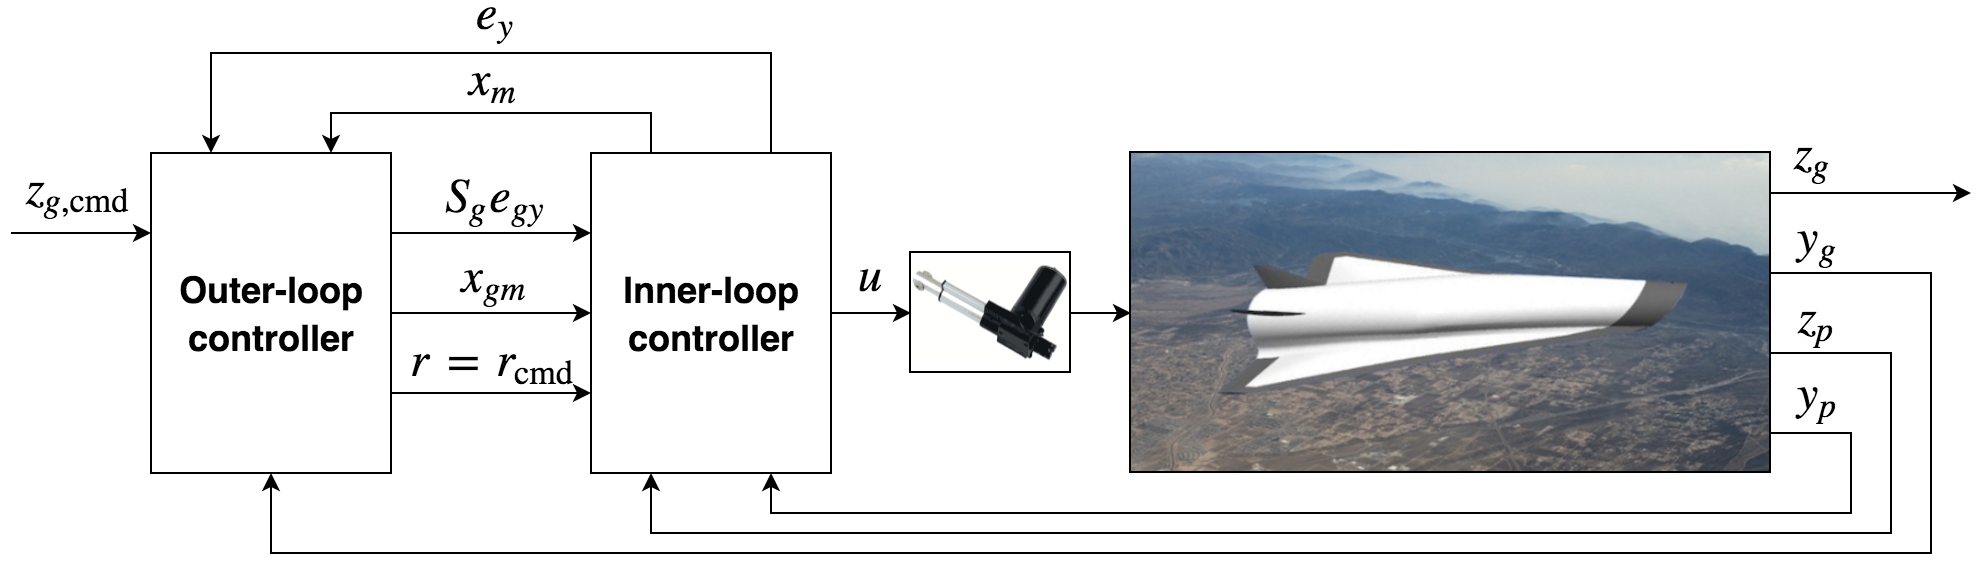
\includegraphics[width=6.5in]{\figurepath/simulationBlock.png}
    \vspace{-0.1in}
    \caption{Simulation block diagram.\label{fig.simblockdiagram}}
  \end{center}
\end{figure}

\subsection{Actuator Models}

\subsubsection{Throttle} The propulsion system is modeled as a first order system with a cutoff frequency of 10 rad/s, with transfer function
\begin{equation*}
  G_{\text{th}}(s)=\frac{\omega_{\text{th}}}{s+{\omega_{\text{th}}}}
\end{equation*}
While the physics of the engine happen on time scales order of magnitude faster than the rest of the dynamics, this simple model was proposed to capture fuel system delivery limits.

\subsubsection{Control Surfaces} Second order actuators with rate and deflection limits were included in the simulation model on all four of the aerodynamic control surfaces.
The transfer function for the control surface actuators is
\begin{equation*}
  G_{\text{cs}}(s)=\frac{{\omega_{n}}^{2}}{s^{2}+2\zeta\omega_{n}s+{\omega_{n}}^{2}}
\end{equation*}
and the block diagram for the control surfaces as implemented is shown in Figure~\ref{fig.actuatorBlock} where the signal $u_{\text{cmd}}$ is generated by the controller, and due to the actuator dynamics the actual control surface deflection is given by $u_{\text{sat}}$.
The relevant values used in the second order aerodynamic control surface actuator model are listed in Table~\ref{tab:actuator}.

\begin{figure}[H]
  \begin{center}
    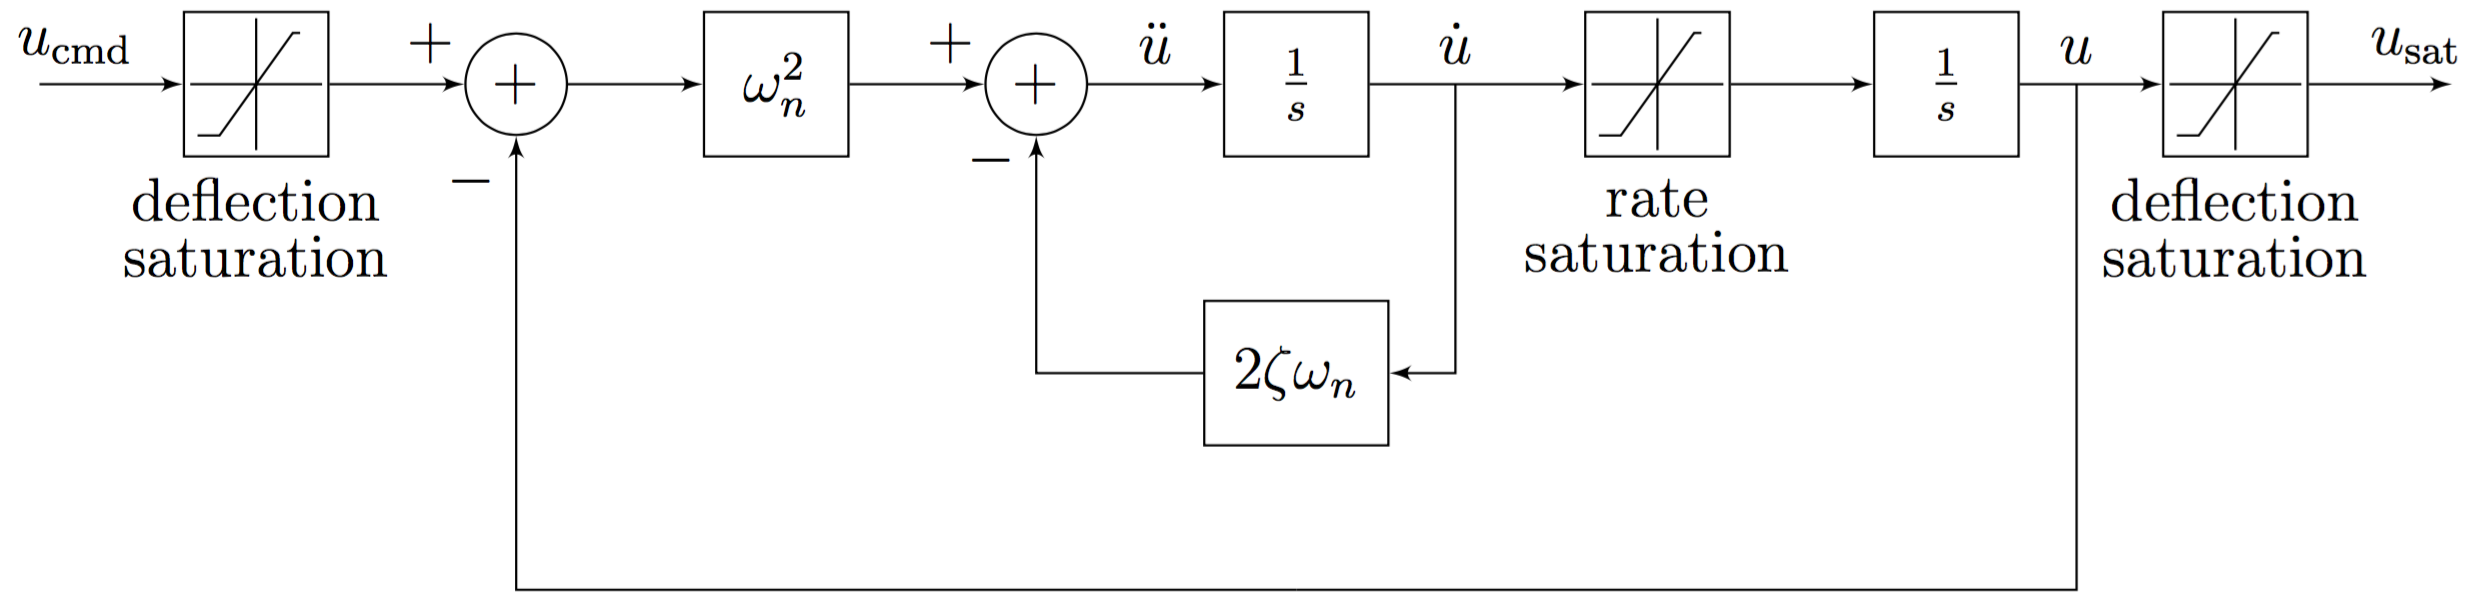
\includegraphics[width=5.5in]{\figurepath/actuatorBlock.png}
    \vspace{-0.1in}
    \caption{Second order actuator dynamics.\label{fig.actuatorBlock}}
  \end{center}
\end{figure}

\begin{table}[H]
  \centering
  \caption{Second order aerodynamic control surface actuator parameters\label{tab:actuator}}
  \begin{tabular}{llc}
    \toprule
    Parameter & Unit & Value \\ \midrule
    Surface deflection limit & [deg] & $-30$ to $30$ \\
    Surface rate limit & [deg/s] & $-100$ to $100$ \\
    Damping ratio $\zeta$ & & $0.7$ \\
    Natural frequency $\omega_{n}$ & [rad/s] & $150$ \\
    \bottomrule
  \end{tabular}
\end{table}

\begin{table}[H]
  \centering
  \caption{Components of trim state vector at nominal flight condition of Mach 5}
  \small
  \begin{tabular}{llr}
    \toprule
    State variable & Units & Value \\ \midrule
    $V_{T}$ & [ft/s] & 5866 \\
    $\alpha$ & [deg] & -0.59 \\
    $q$ & [deg/s] & 0 \\
    $\theta$ & [deg] & -0.59 \\
    $h$ & [ft] & 80,000 \\
    $\beta$ & [deg] & 0 \\
    $p$ & [deg/s] & 0 \\
    $r$ & [deg/s] & 0 \\
    $\phi$ & [deg] & 0 \\ \bottomrule
  \end{tabular}\label{tab:trimstate}
\end{table}

\section{Simulation Results}

The performance and robustness of the inner-loop adaptive controllers synthesized using the design model as represented by Eq.\ \eqref{eqn.xdotpunc} were evaluated by applying these controllers to an evaluation model\textemdash{}the hypersonic vehicle which is nonlinear and includes second order dynamics on the actuators which actuate the elevators, ailerons, and rudders, and the throttle response modeled as first order.
The numerical property values are listed in Table~\ref{tab:actuator}.
Uncertainties were introduced in the nonlinear model, which manifest themselves in the uncertain linear system as given in Eq.\ \eqref{eqn.xdotpunc}.
The uncertainty is as follows:
\begin{itemize}
  \item{Control effectiveness on all surfaces is reduced to 20\% of the nominal value.}
  \item{Center of gravity is shifted 0.7 feet rearward, effectively representing uncertainty in the center-of-pressure location.}
  \item{The rolling moment coefficient $C_{l}$ is reduced to 10\% of the nominal value.}
\end{itemize}

\subsection{Inner-Loop Response}\label{sec.numericalExample.innerLoop}

To evaluate the response of the inner-loop longitudinal controller, a 2 deg/s pitch rate doublet command was given.
The nominal response of the aircraft is shown in Figure~\ref{fig.baselineInnerNominalLongState} with the corresponding control inputs shown in~\ref{fig.baselineInnerNominalLongControl} for the case with no uncertainty and when using the baseline controller: $\Theta(t)=0$.
To evaluate the response of the lateral-directional controller, a 5 deg/s roll rate doublet command was given.
The nominal response of the aircraft is shown in Figure~\ref{fig.baselineInnerNominalLatrState} with the corresponding control inputs shown in Figure~\ref{fig.baselineInnerNominalLatrControl} for the case with no uncertainty and when using the baseline controller: $\Theta(t)=0$.

The purposed of both these inner-loop simulation responses is to show the nominal command tracking performance.
The introduction of uncertainty ultimately destabilizes the system when using the baseline controller, with the adaptive controller able to restore stability and ensure command tracking in the presence of these uncertainties.
However, to better examine the effect of these uncertainties on the vehicle performance when using both the baseline and adaptive controllers, this was done when using the outer-loop controller as well, as shown in the following section.

\newpage
\begin{figure}[H]
  \hspace{-0.5in}
  \noindent\makebox[7.5in]{%
  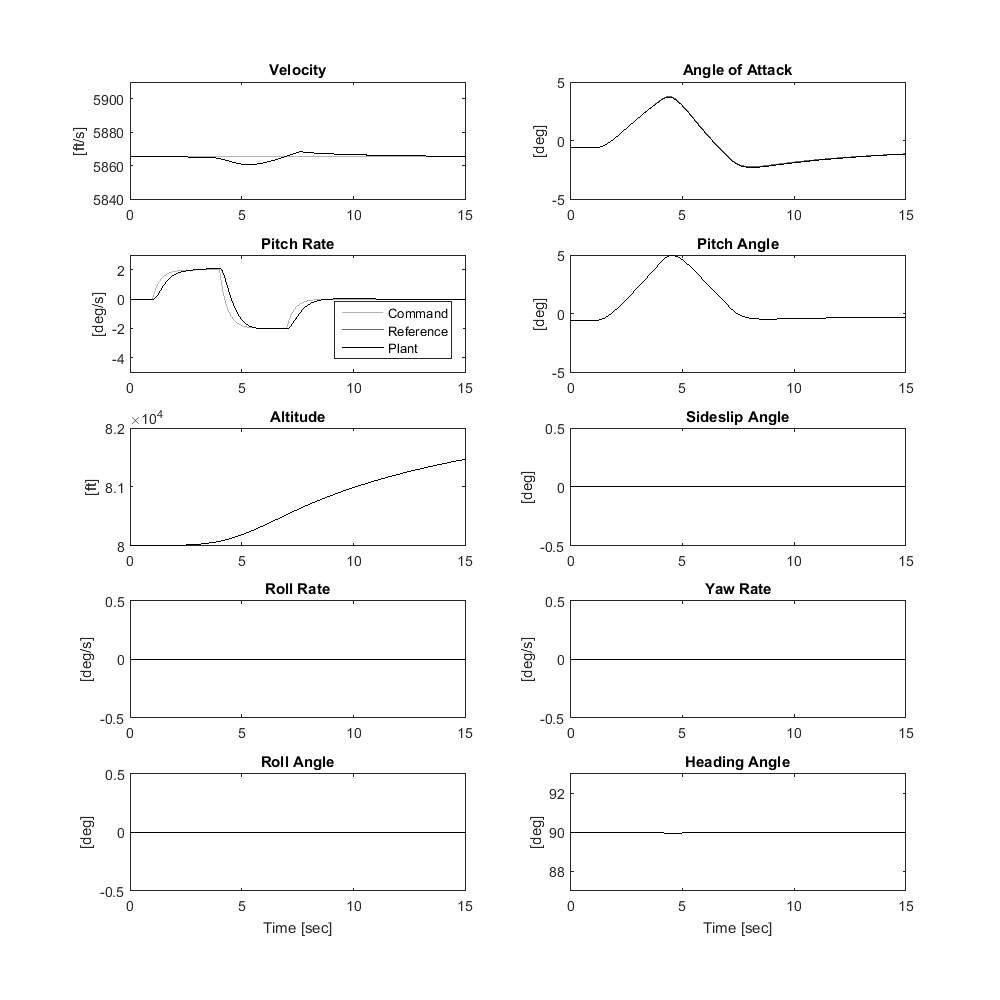
\includegraphics[width=7.5in]{\figurepath/baselineInnerNominalLongState.png}}
  \vspace{-1.0in}
  \caption{Plant states for baseline controller applied to nominal plant in response to a 2 degree per second pitch rate doublet.\label{fig.baselineInnerNominalLongState}}
\end{figure}

\newpage
\begin{figure}[H]
  \hspace{-0.5in}
  \noindent\makebox[7.5in]{%
  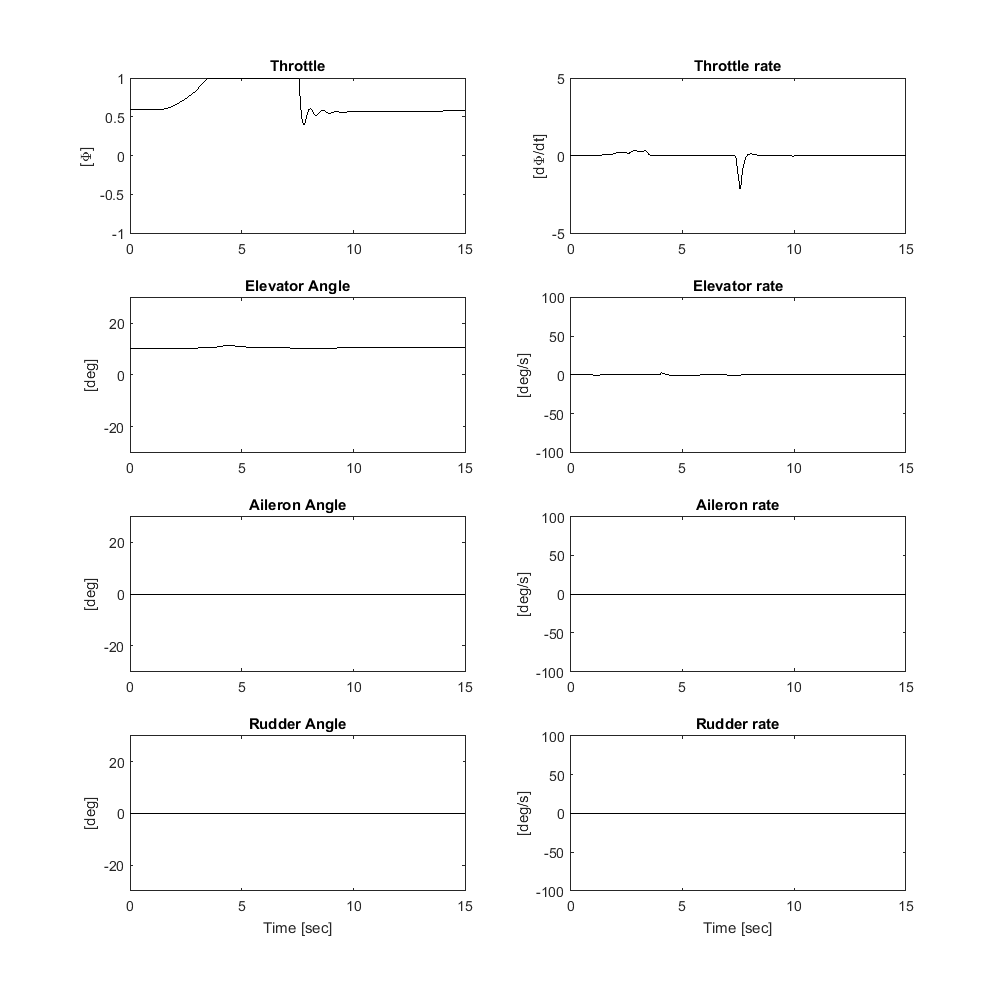
\includegraphics[width=7.5in]{\figurepath/baselineInnerNominalLongControl.png}}
  \vspace{-1.0in}
  \caption{Plant control input for baseline controller applied to nominal plant in response to a 2 degree per second pitch rate doublet.\label{fig.baselineInnerNominalLongControl}}
\end{figure}

\newpage
\begin{figure}[H]
  \hspace{-0.5in}
  \noindent\makebox[7.5in]{%
  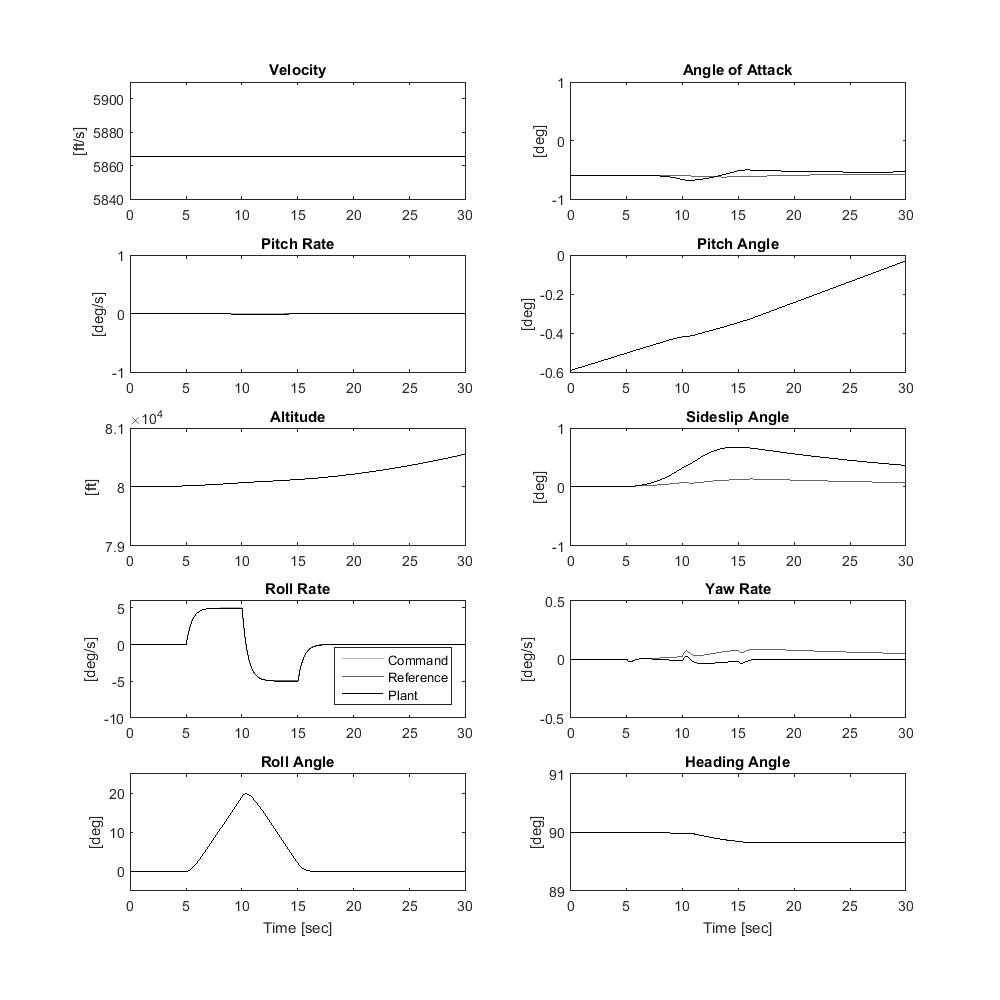
\includegraphics[width=7.5in]{\figurepath/baselineInnerNominalLatrState.png}}
  \vspace{-1.0in}
  \caption{Plant states for baseline controller applied to nominal plant in response to a 5 degree per second roll rate doublet.\label{fig.baselineInnerNominalLatrState}}
\end{figure}

\newpage
\begin{figure}[H]
  \hspace{-0.5in}
  \noindent\makebox[7.5in]{%
  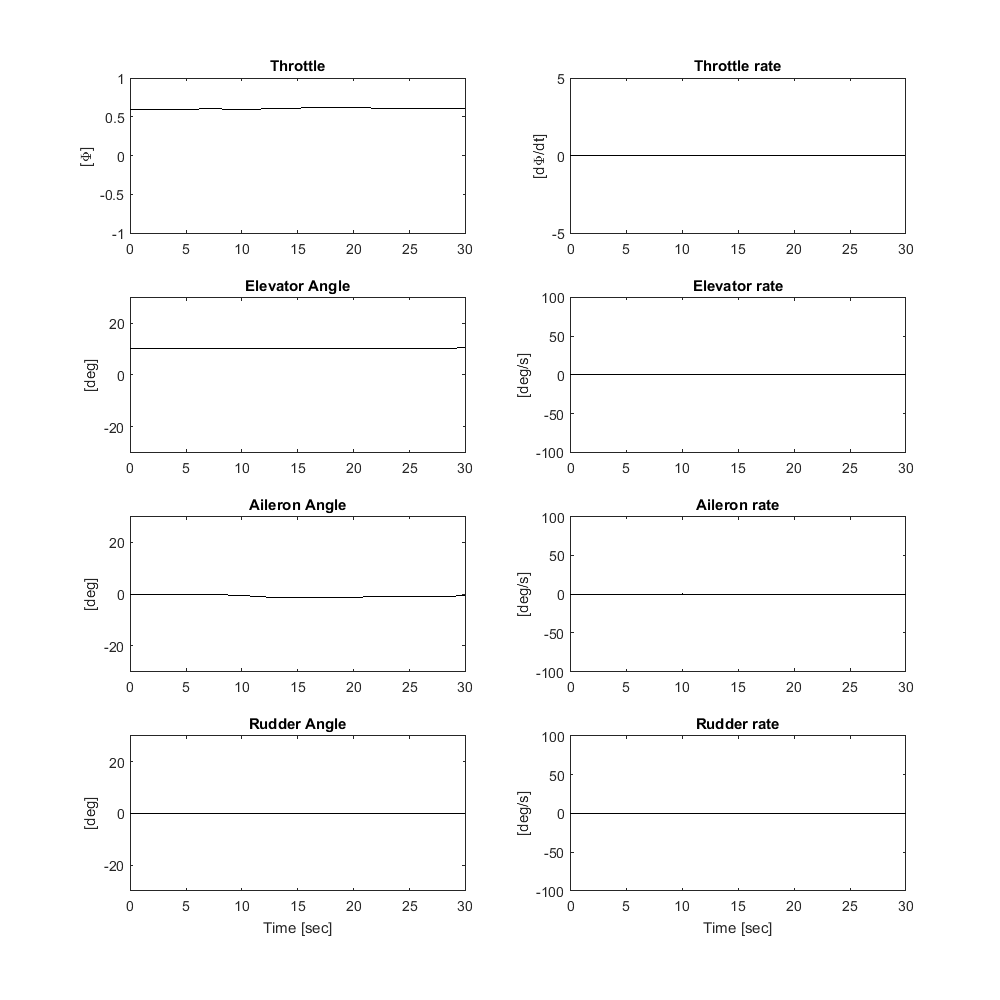
\includegraphics[width=7.5in]{\figurepath/baselineInnerNominalLatrControl.png}}
  \vspace{-1.0in}
  \caption{Plant control input for baseline controller applied to nominal plant in response to a 5 degree per second roll rate doublet.\label{fig.baselineInnerNominalLatrControl}}
\end{figure}


\subsection{Outer-Loop Response}\label{sec.numericalExample.outerLoop}

With the command tracking performance of the inner-loop controller verified in Sec.~\ref{sec.numericalExample.innerLoop}, the outer-loop was then designed around this inner-loop as described in Ch.~\ref{ch.outerLoop}.
The performance of the combined inner and outer-loop control structure was evaluated for both the longitudinal and lateral-directional control subsystems.

\subsubsection{Longitudinal Response}

To evaluate the longitudinal response of the GHV when using the closed-loop controllers, an altitude command to climb 1000 ft was given.
Figs.~\ref{fig.baselineNominalLongState} and~\ref{fig.baselineNominalLongControl} show the response in the nominal case, corresponding to the absence of uncertainty, and no adaptive control used.
That is $\Lambda=I$, $\Psi_{p}=0$, and $\Theta(t)=0$.
The response shows a smooth climb to the new altitude, while maintaining the desired heading, and without requiring large control magnitudes or rates.

Figs.~\ref{fig.baselineUncertainLongState} and~\ref{fig.baselineUncertainLongControl} show the response when the uncertainty was introduced, but with the adaptive controller still not used, that is $\Theta(t)=0$.
In this case, the uncertainty is sufficient to destabilize the GHV within a matter of seconds.

Figs.~\ref{fig.adaptiveUncertainLongState} and~\ref{fig.adaptiveUncertainLongControl} show the response when the adaptive controller is turned on. The result of this is closed-loop stability, and tracking of the altitude command.
However, during the course of adaptation some large undesirable oscillations are observed.

\subsubsection{Lateral-Directional Response}

To evaluate the lateral-direction response of the GHV when using the closed-loop controllers, a heading command of a right turn of 5 degrees was given.
Figs.~\ref{fig.baselineNominalLatrState} and~\ref{fig.baselineNominalLatrControl} show the response in the nominal case, corresponding to the absence of uncertainty, and no adaptive control used.
That is $\Lambda=I$, $\Psi_{p}=0$, and $\Theta(t)=0$.
The response shows a smooth turn to the new heading, while maintaining the desired altitude, and without requiring large control magnitudes or rates.

Figs.~\ref{fig.baselineUncertainLatrState} and~\ref{fig.baselineUncertainLatrControl} show the response when the uncertainty was introduced, but with the adaptive controller still not used, that is $\Theta(t)=0$.
In this case, the uncertainty is sufficient to destabilize the GHV within a matter of seconds.

Figs.~\ref{fig.adaptiveUncertainLatrState} and~\ref{fig.adaptiveUncertainLatrControl} show the response when the adaptive controller is turned on.
The result of this is closed-loop stability, and tracking of the heading command.
However, during the course of adaptation some large undesirable oscillations are observed.

\newpage
\begin{figure}[H]
  \hspace{-0.5in}
  \noindent\makebox[7.5in]{%
  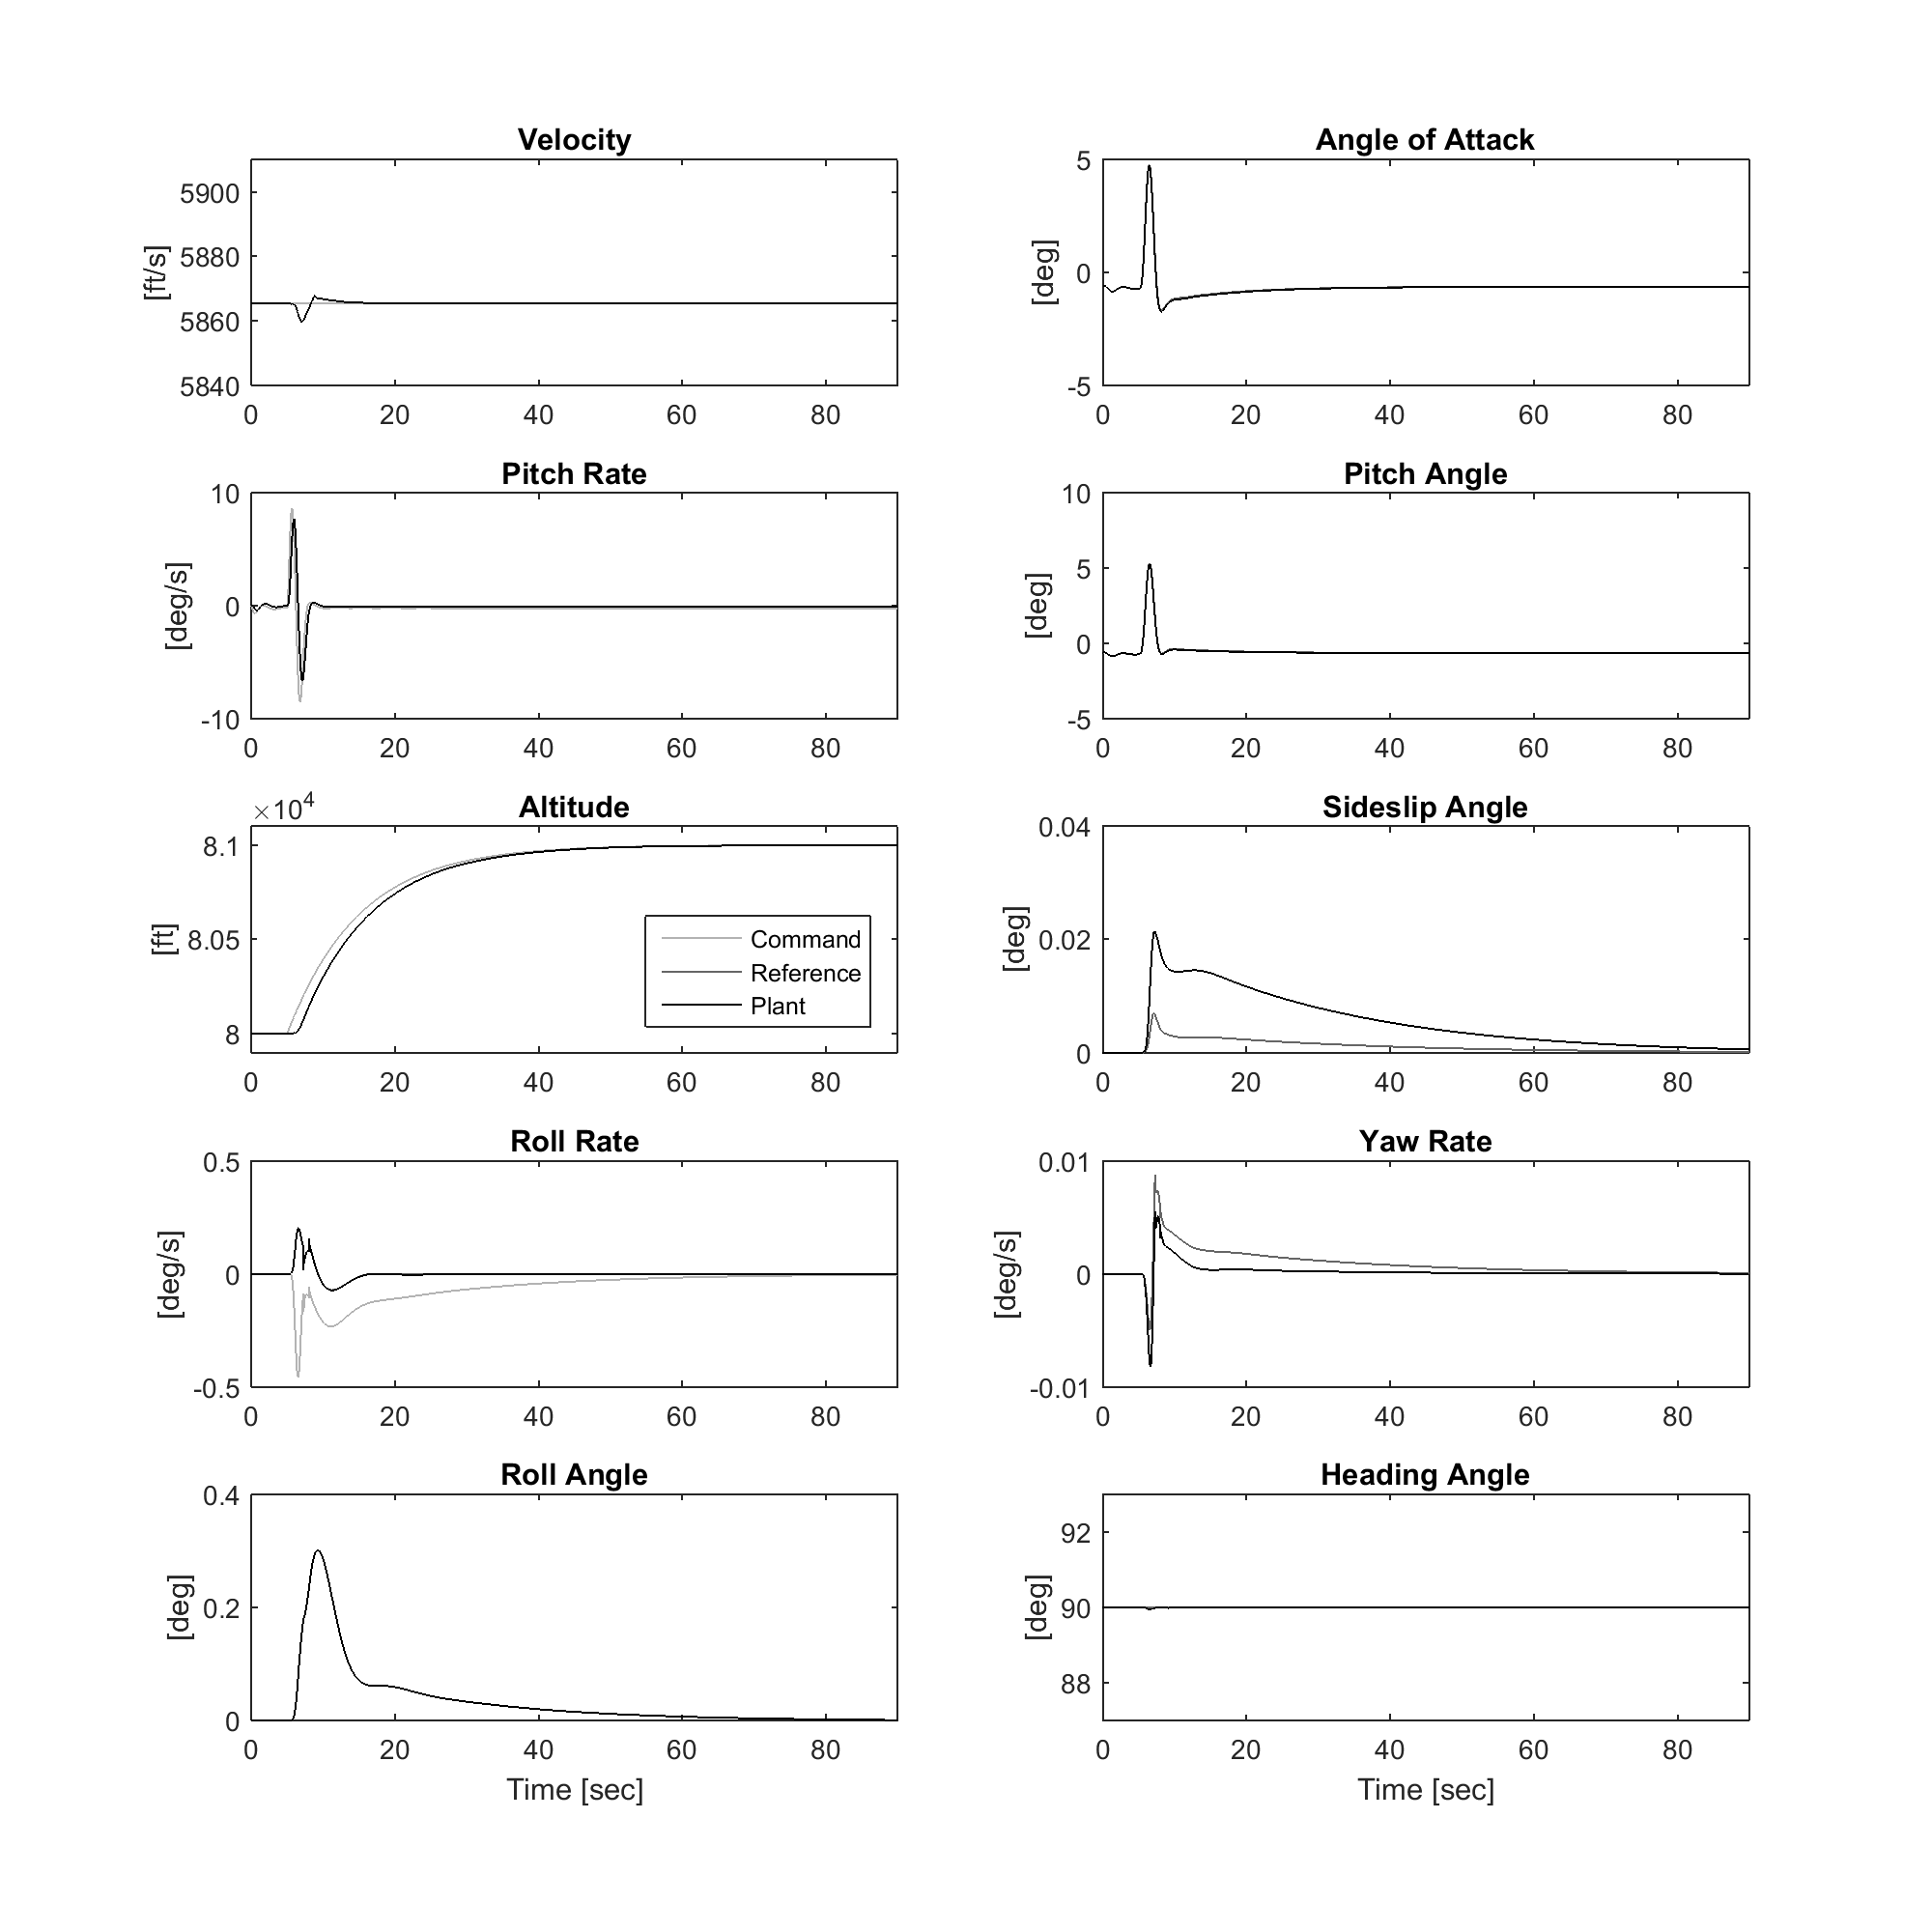
\includegraphics[width=7.5in]{\figurepath/baselineNominalLongState.png}}
  \vspace{-1.0in}
  \caption{Plant states for baseline controller applied to nominal plant in response to a 1000 ft.\ climb command.\label{fig.baselineNominalLongState}}
\end{figure}

\newpage
\begin{figure}[H]
  \hspace{-0.5in}
  \noindent\makebox[7.5in]{%
  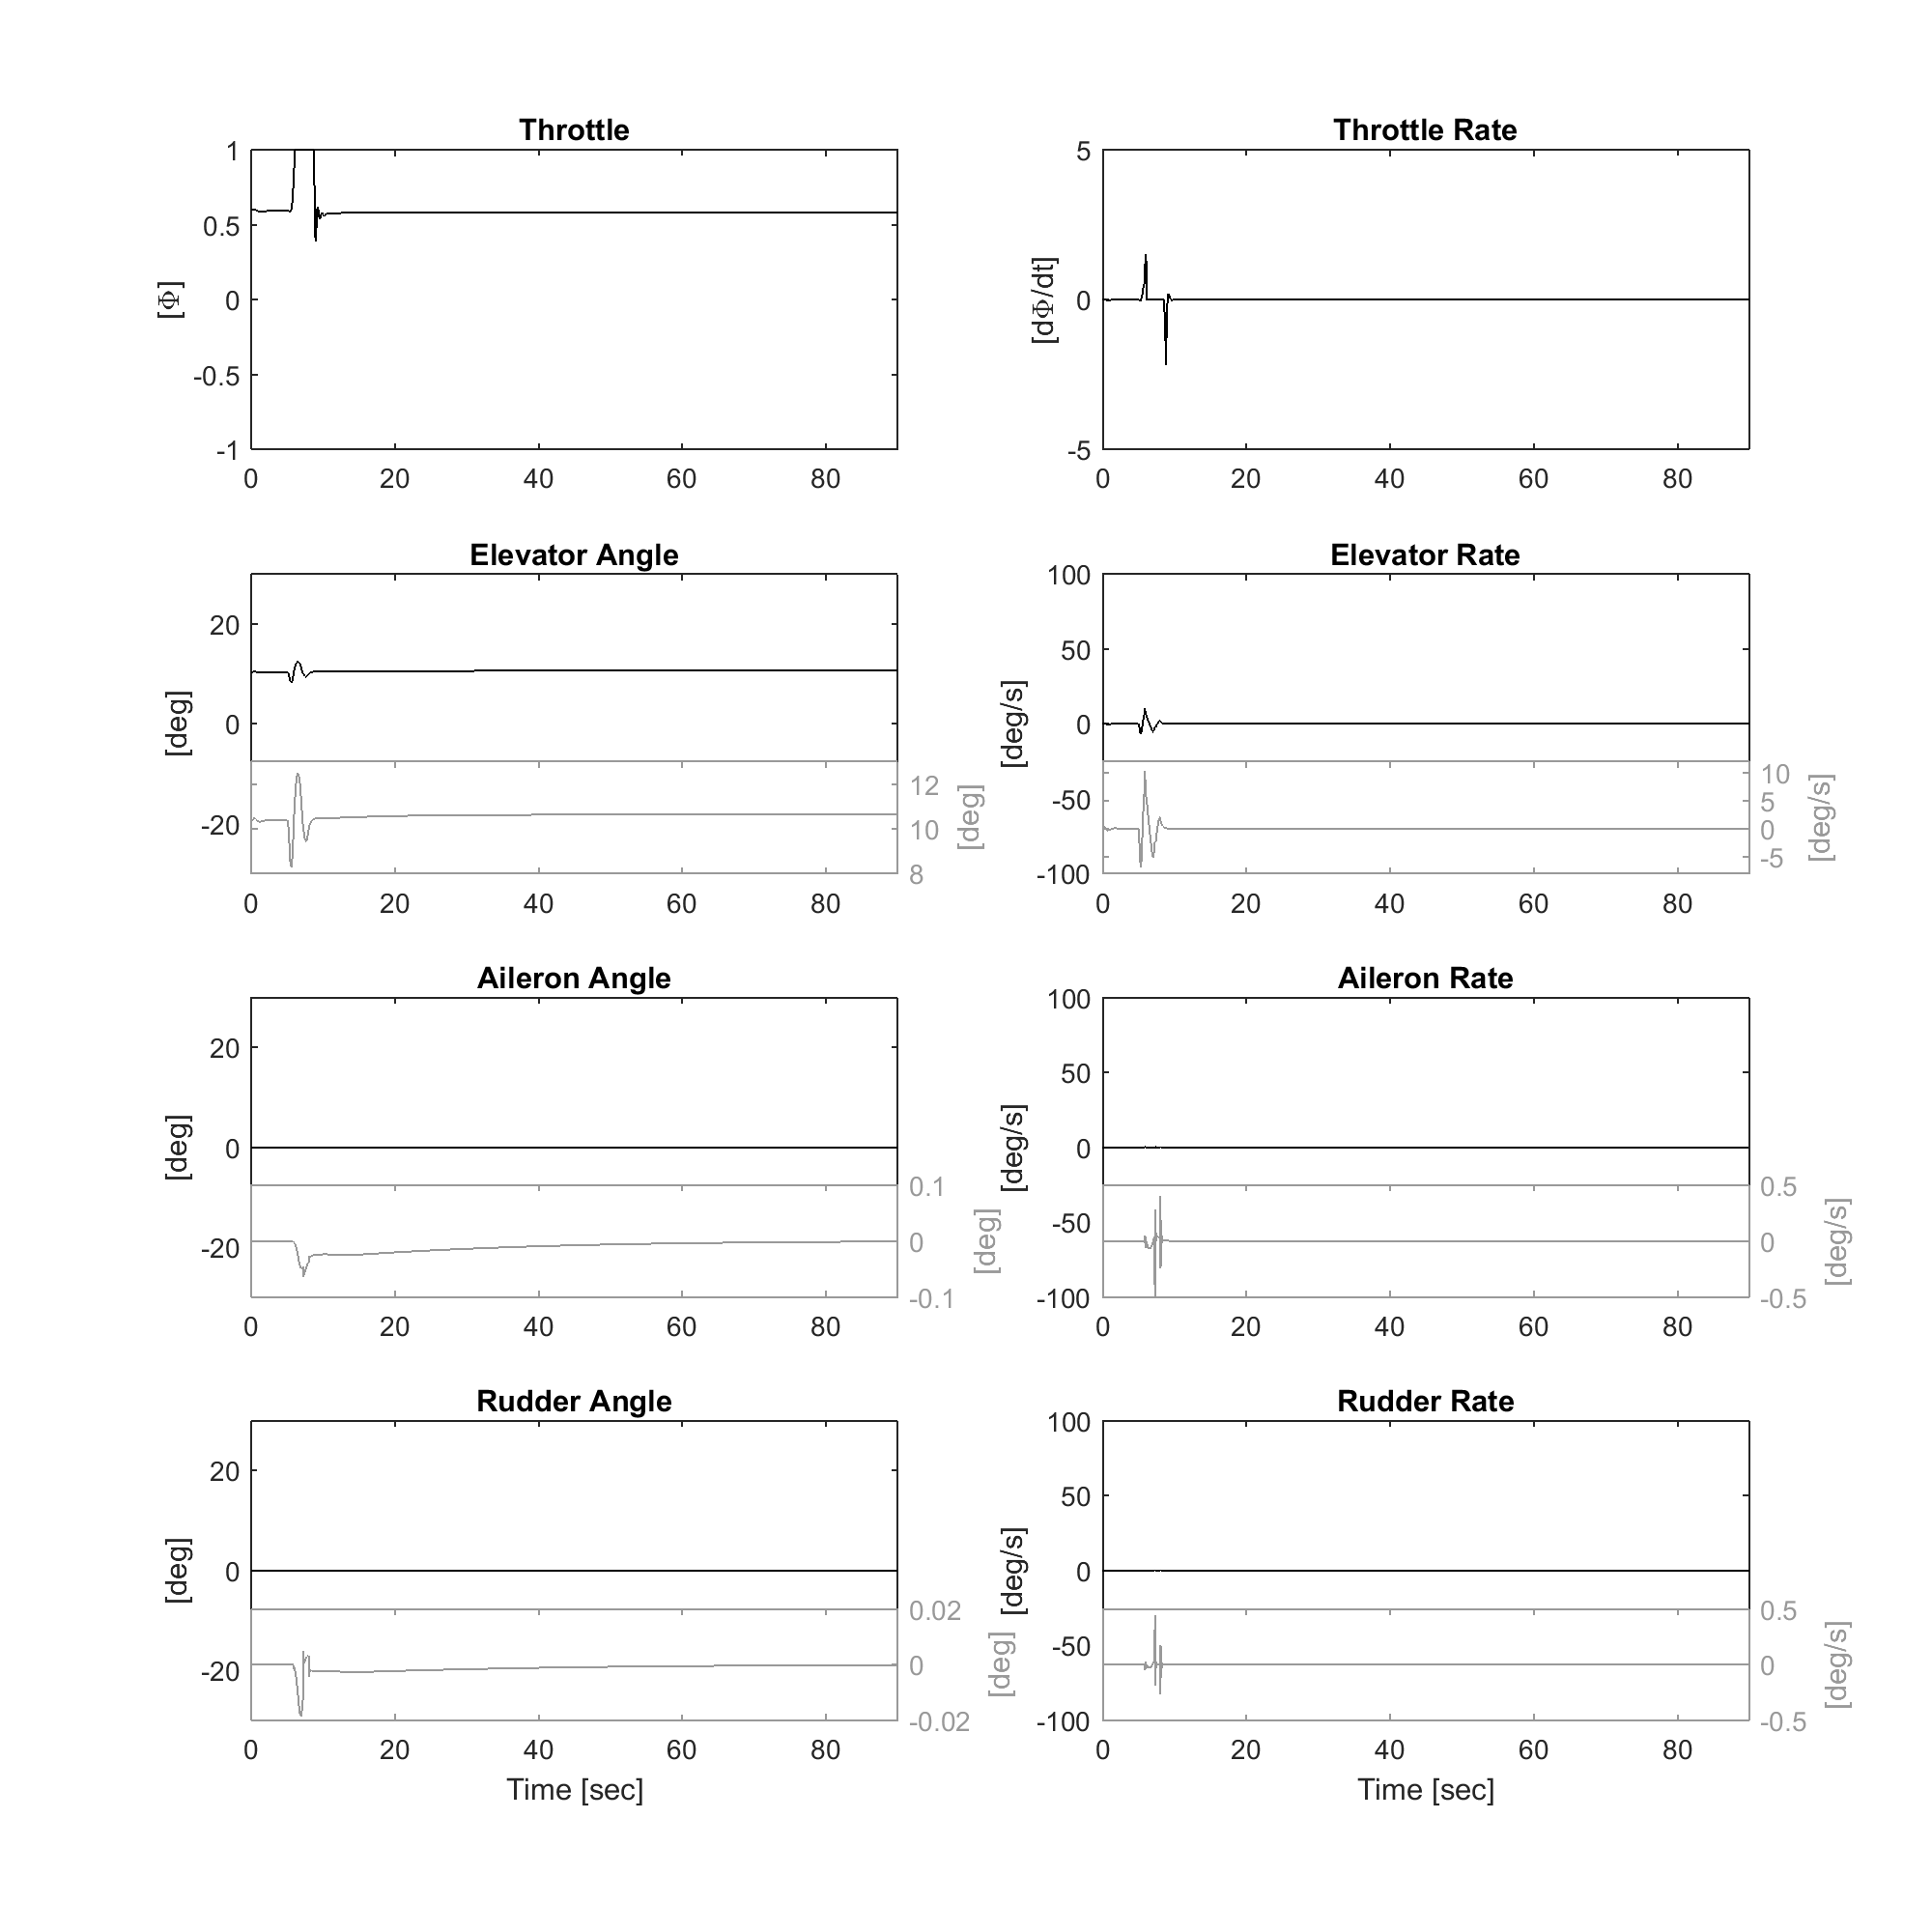
\includegraphics[width=7.5in]{\figurepath/baselineNominalLongControl.png}}
  \vspace{-1.0in}
  \caption{Plant control input for baseline controller applied to nominal plant in response to a 1000 ft.\ climb command.\label{fig.baselineNominalLongControl}}
\end{figure}

\newpage
\begin{figure}[H]
  \hspace{-0.5in}
  \noindent\makebox[7.5in]{%
  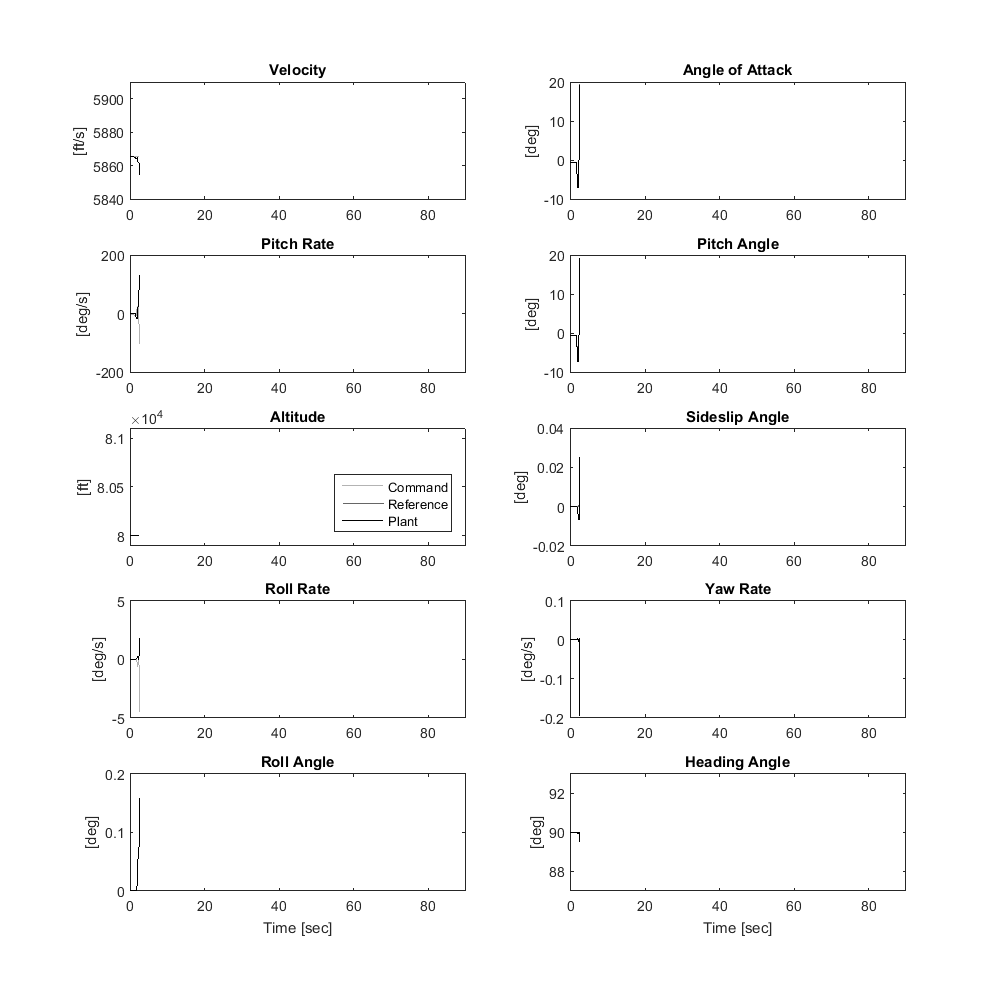
\includegraphics[width=7.5in]{\figurepath/baselineUncertainLongState.png}}
  \vspace{-1.0in}
  \caption{Plant states for baseline controller applied to uncertain plant in response to a 1000 ft.\ climb command.\label{fig.baselineUncertainLongState}}
\end{figure}

\newpage
\begin{figure}[H]
  \hspace{-0.5in}
  \noindent\makebox[7.5in]{%
  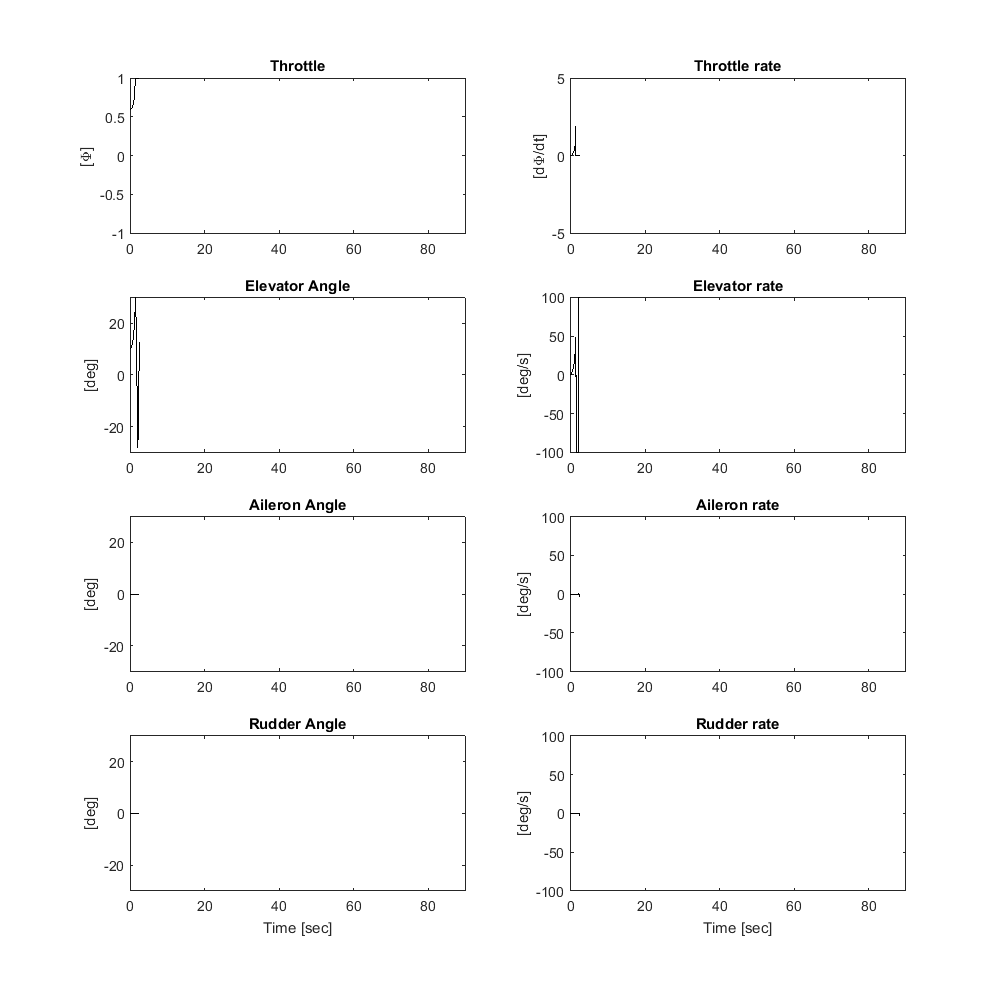
\includegraphics[width=7.5in]{\figurepath/baselineUncertainLongControl.png}}
  \vspace{-1.0in}
  \caption{Plant control input for baseline controller applied to uncertain plant in response to a 1000 ft.\ climb command.\label{fig.baselineUncertainLongControl}}
\end{figure}

\newpage
\begin{figure}[H]
  \hspace{-0.5in}
  \noindent\makebox[7.5in]{%
  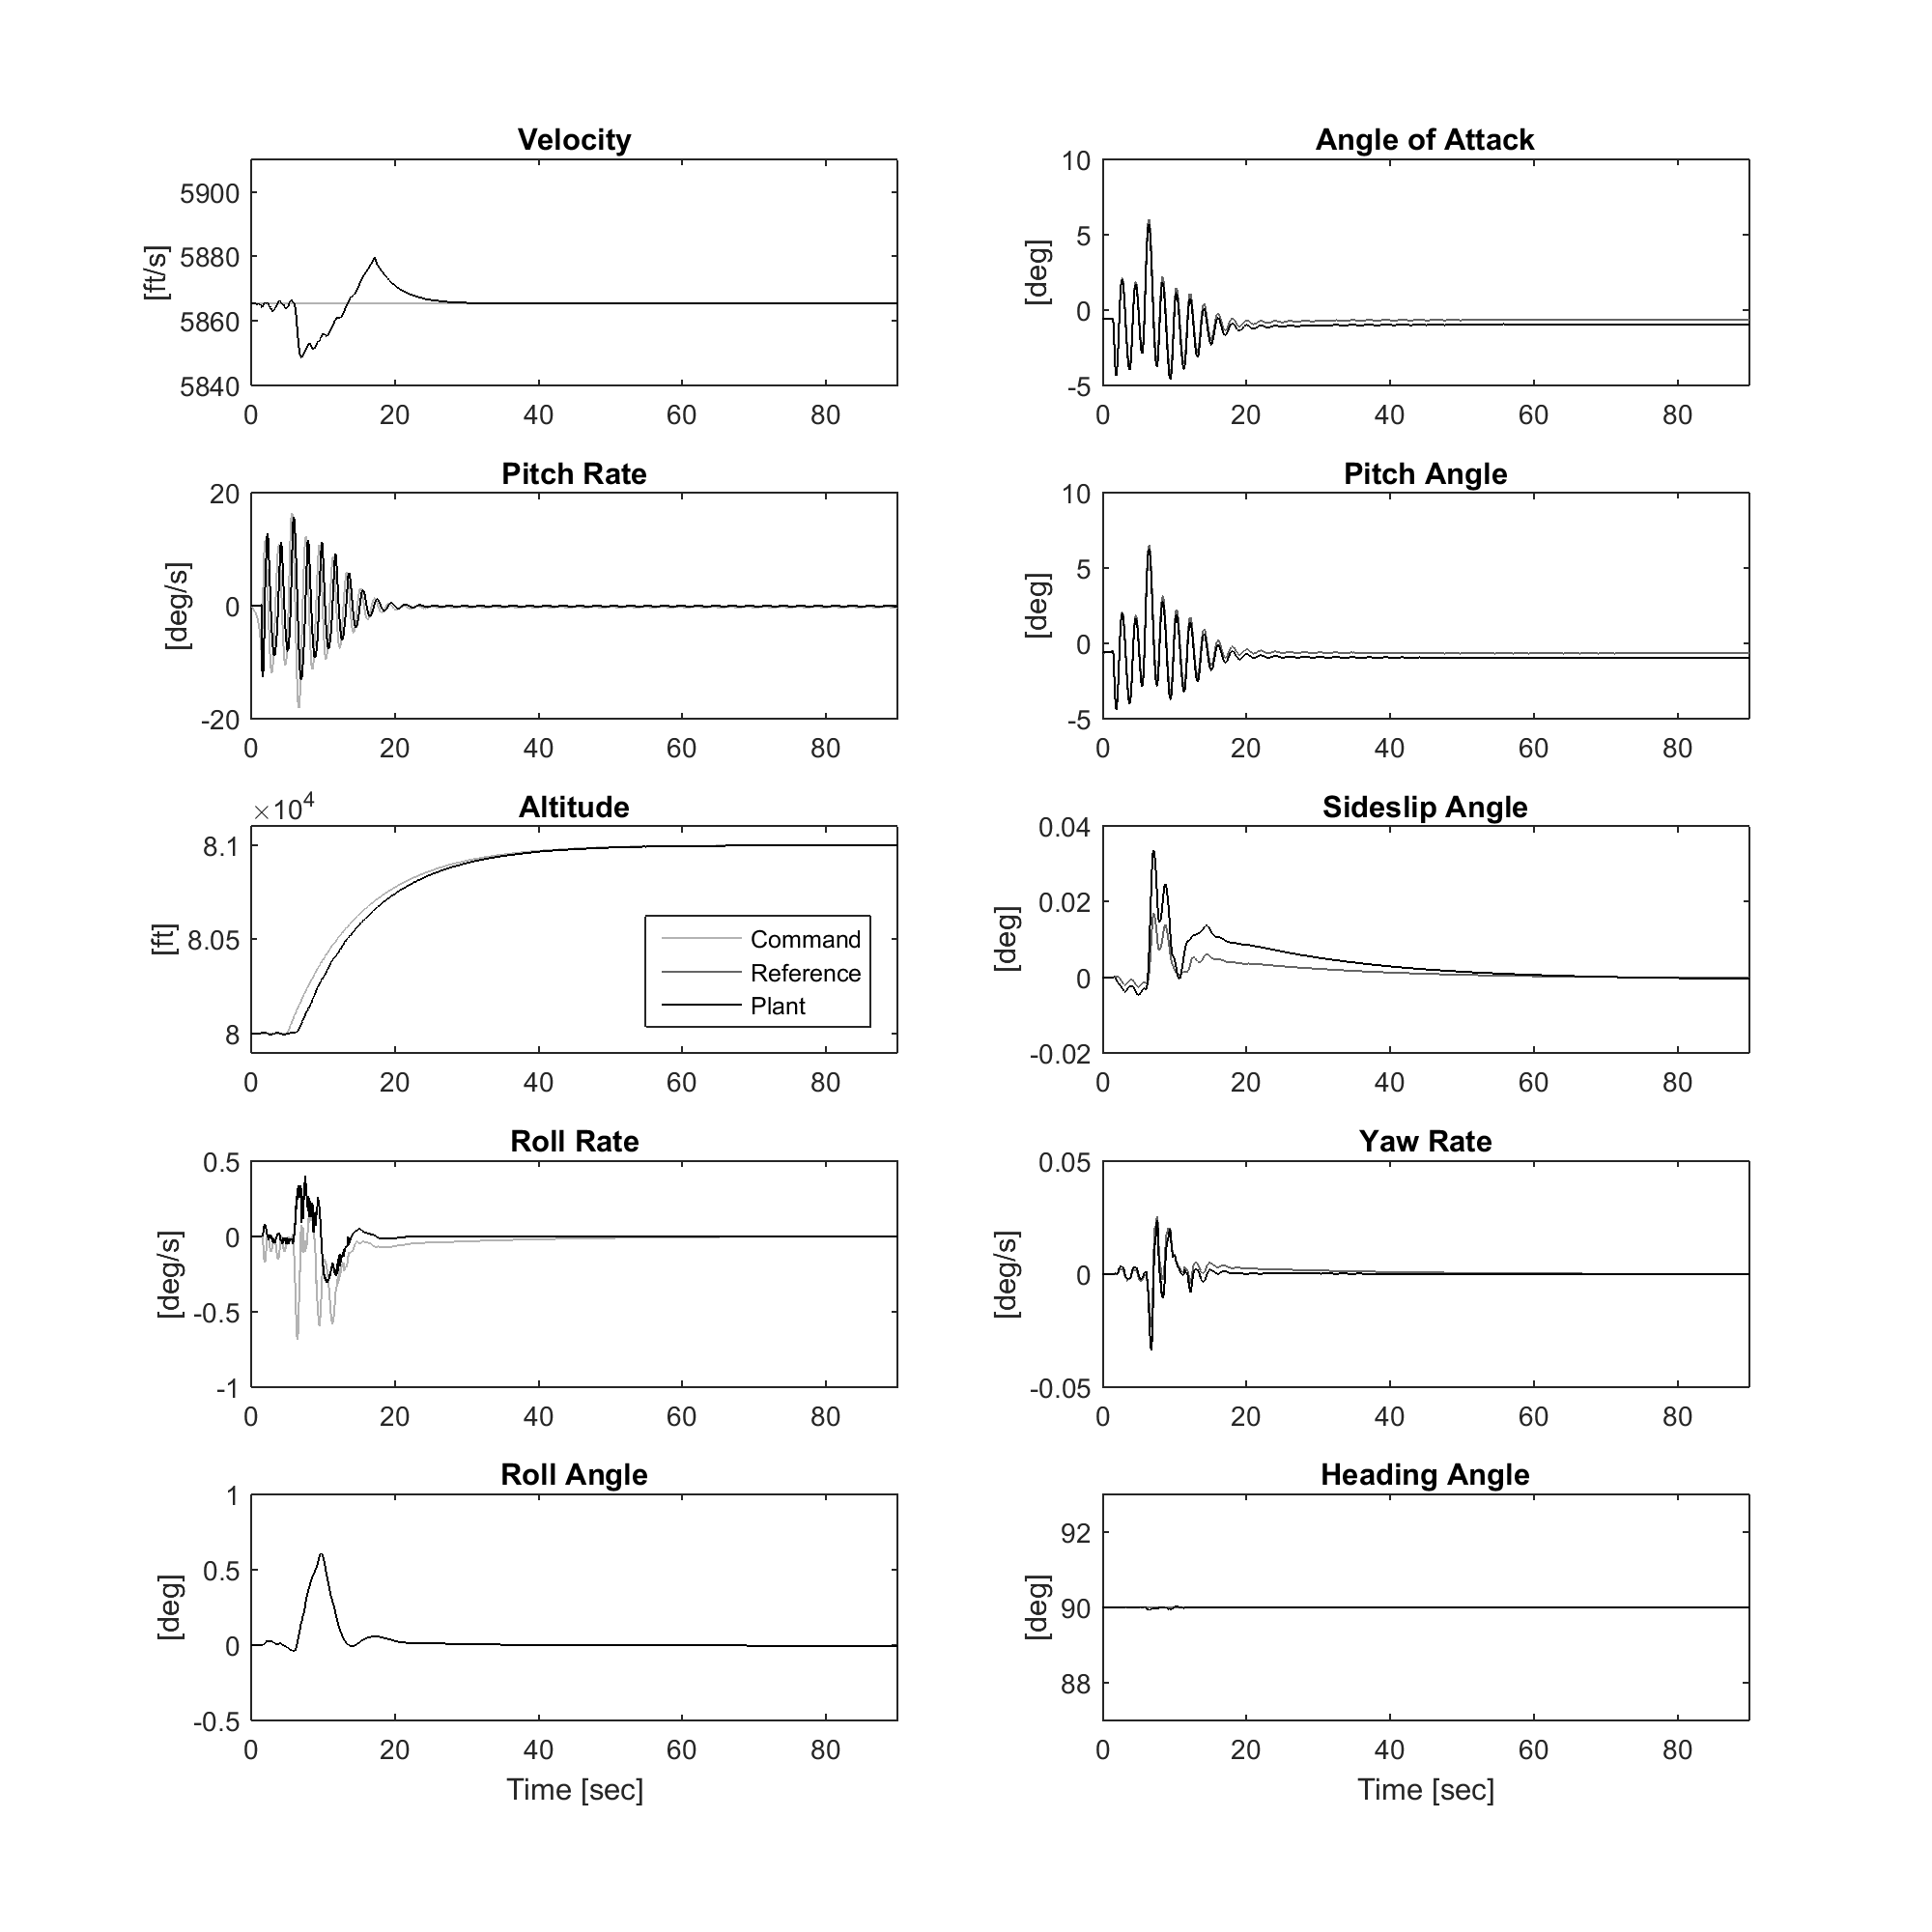
\includegraphics[width=7.5in]{\figurepath/adaptiveUncertainLongState.png}}
  \vspace{-1.0in}
  \caption{Plant states for adaptive controller applied to uncertain plant in response to a 1000 ft.\ climb command.\label{fig.adaptiveUncertainLongState}}
\end{figure}

\newpage
\begin{figure}[H]
  \hspace{-0.5in}
  \noindent\makebox[7.5in]{%
  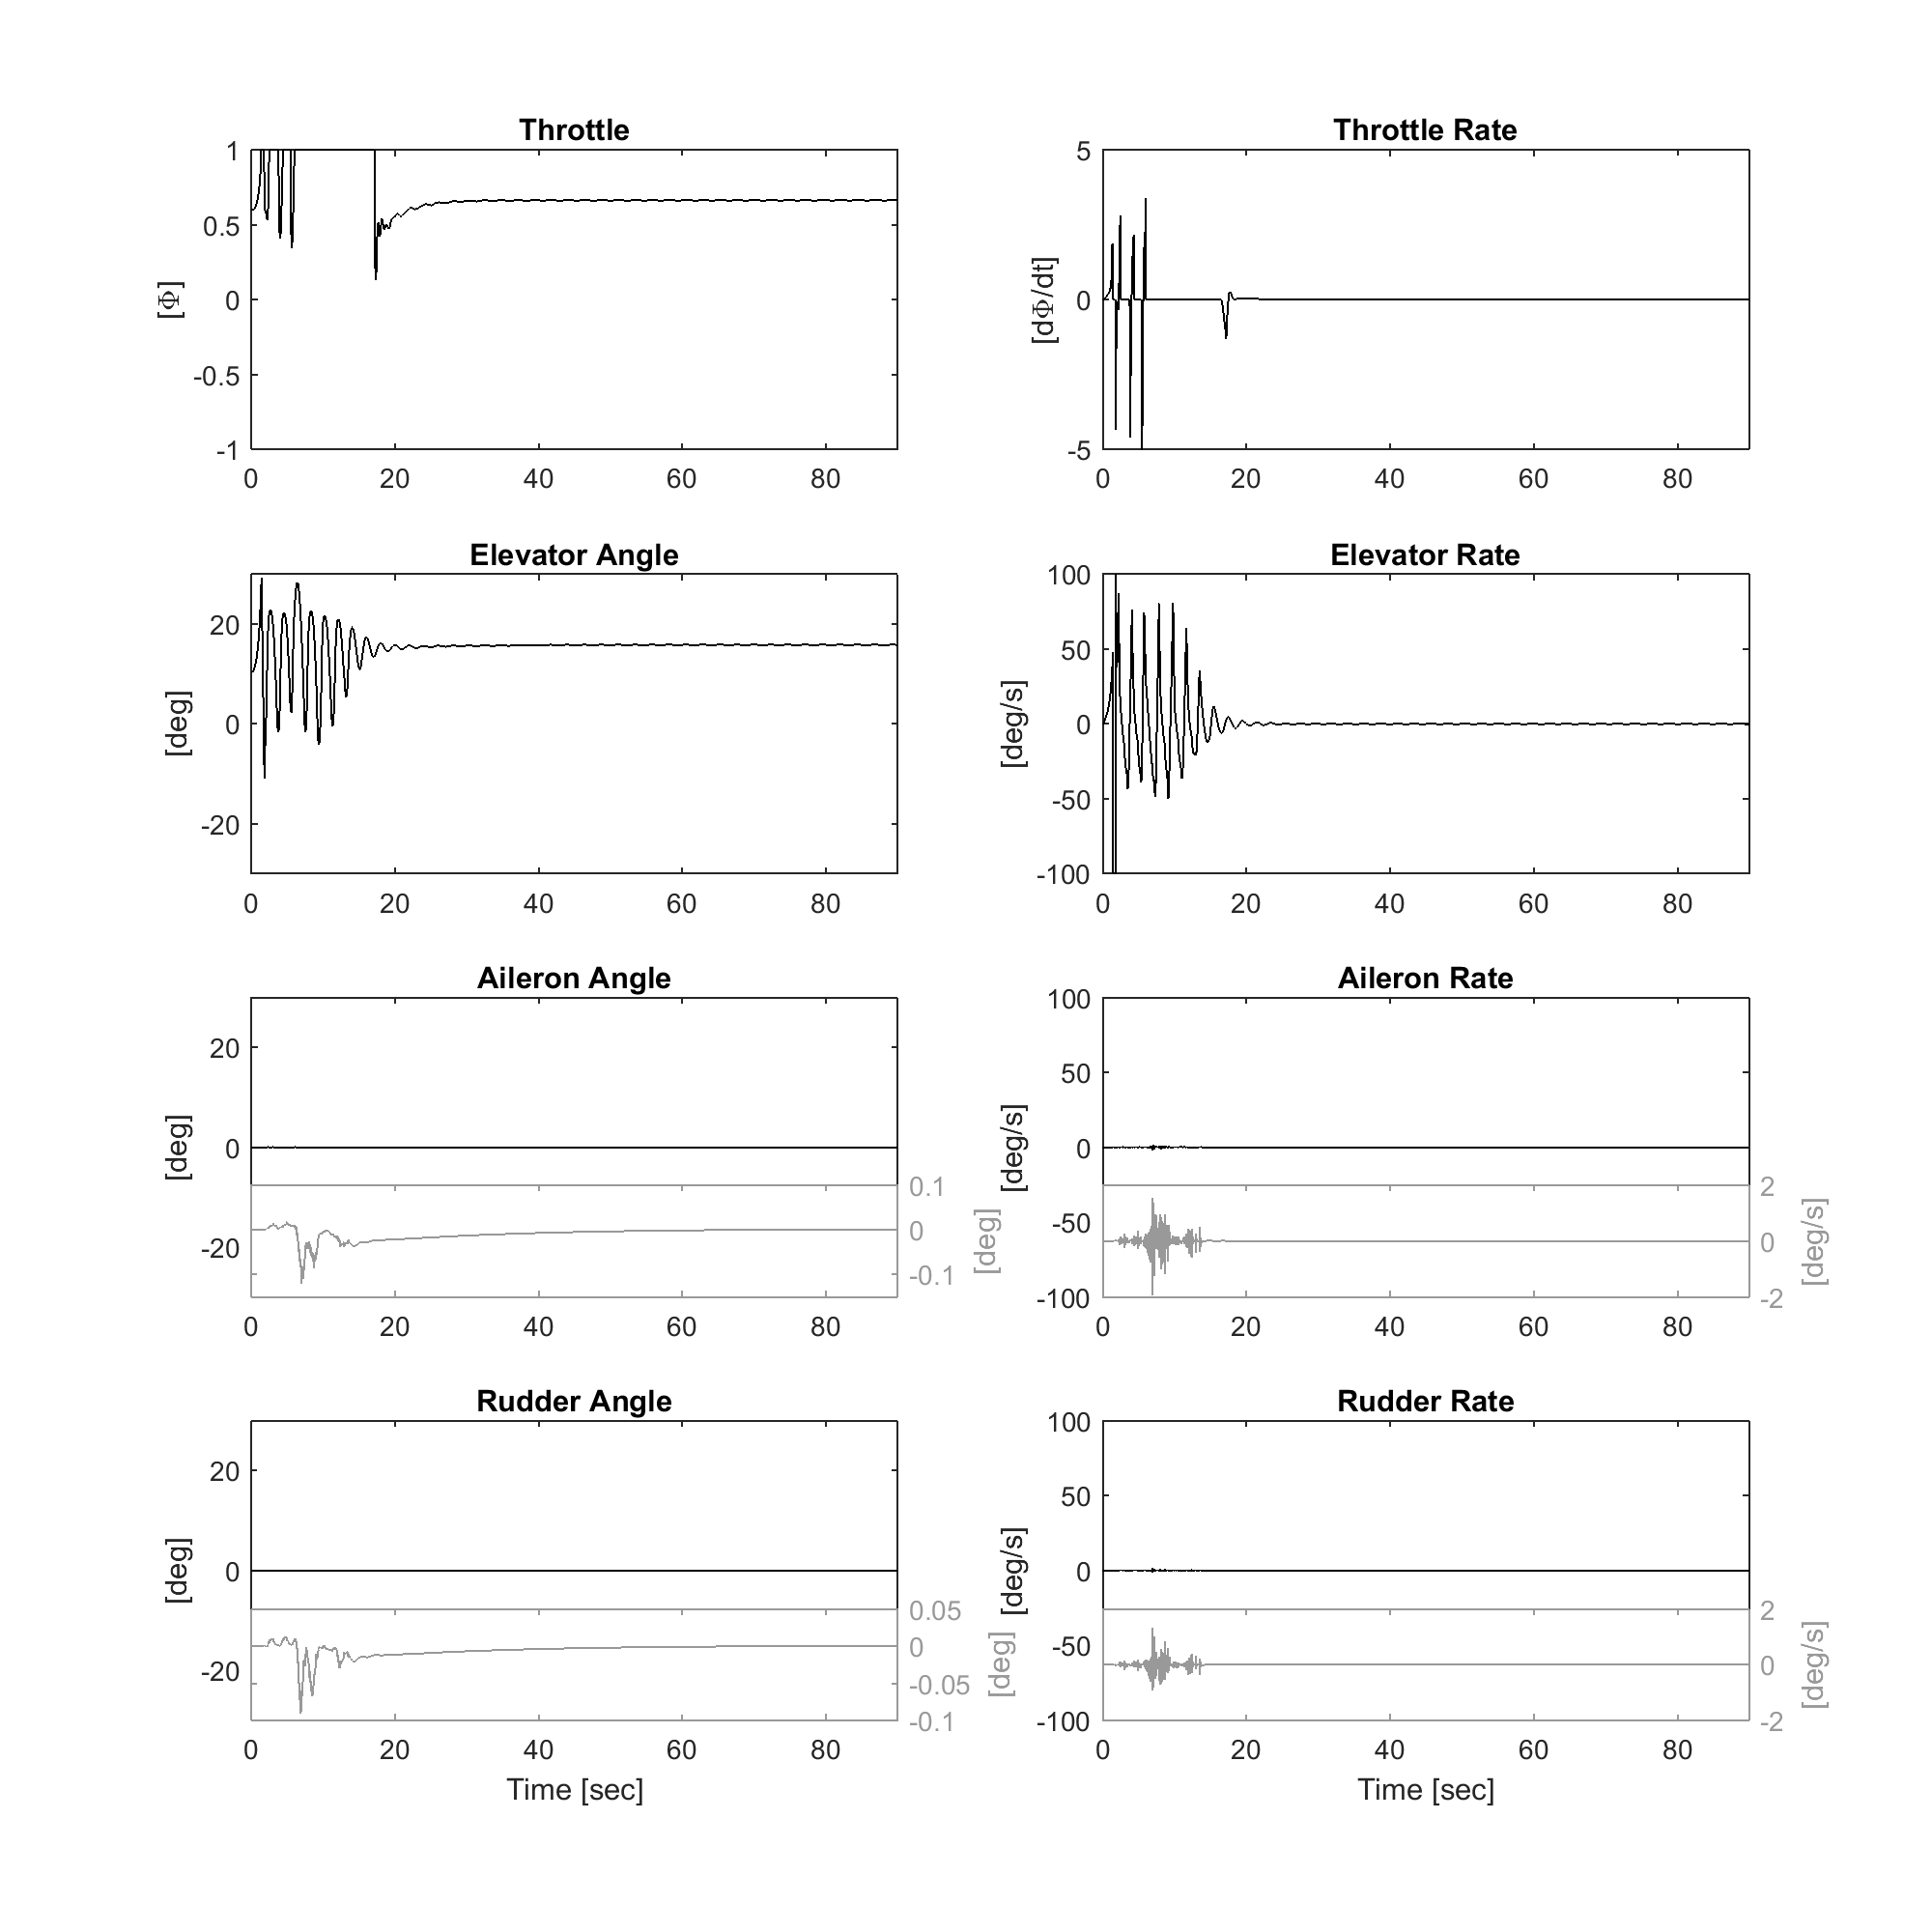
\includegraphics[width=7.5in]{\figurepath/adaptiveUncertainLongControl.png}}
  \vspace{-1.0in}
  \caption{Plant control input for adaptive controller applied to uncertain plant in response to a 1000 ft.\ climb command.\label{fig.adaptiveUncertainLongControl}}
\end{figure}

\newpage
\begin{figure}[H]
  \hspace{-0.5in}
  \noindent\makebox[7.5in]{%
  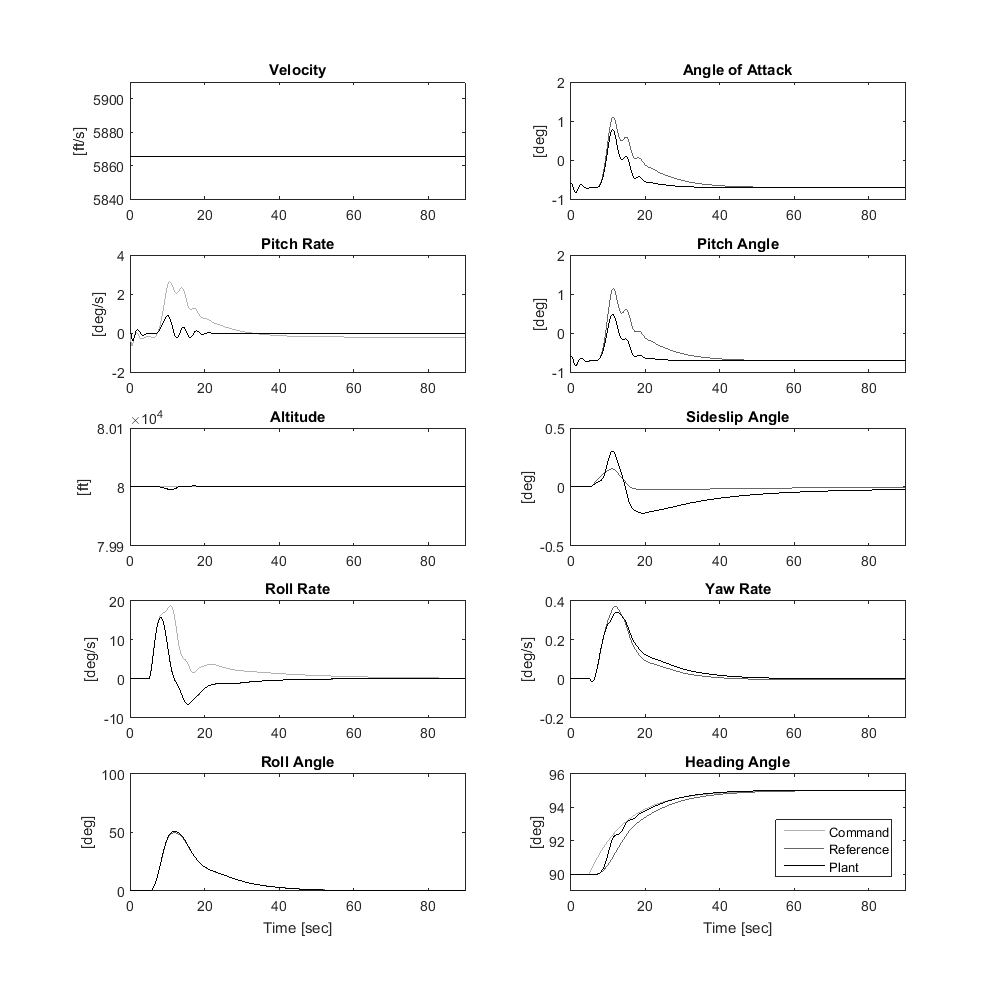
\includegraphics[width=7.5in]{\figurepath/baselineNominalLatrState.png}}
  \vspace{-1.0in}
  \caption{Plant states for baseline controller applied to nominal plant in response to a 5 degree heading turn.\label{fig.baselineNominalLatrState}}
\end{figure}

\newpage
\begin{figure}[H]
  \hspace{-0.5in}
  \noindent\makebox[7.5in]{%
  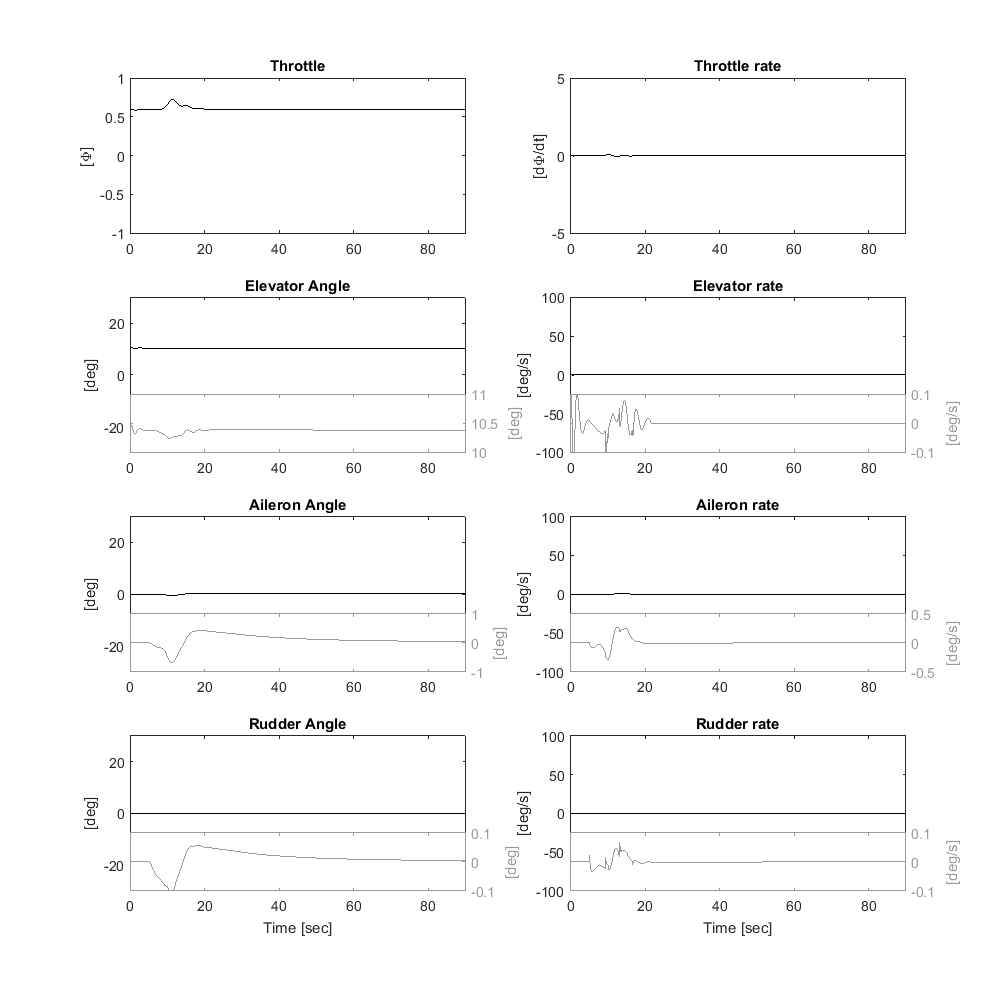
\includegraphics[width=7.5in]{\figurepath/baselineNominalLatrControl.png}}
  \vspace{-1.0in}
  \caption{Plant control input for baseline controller applied to nominal plant in response to a 5 degree heading turn.\label{fig.baselineNominalLatrControl}}
\end{figure}

\newpage
\begin{figure}[H]
  \hspace{-0.5in}
  \noindent\makebox[7.5in]{%
  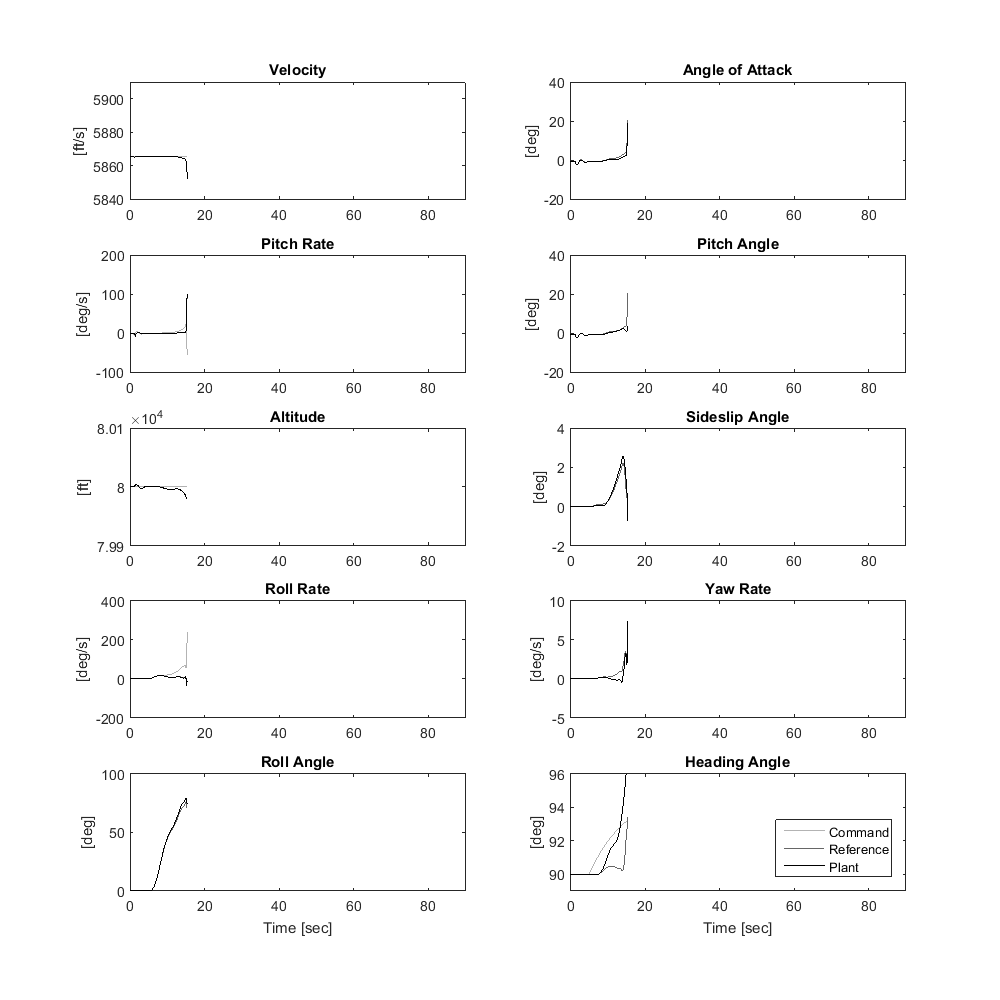
\includegraphics[width=7.5in]{\figurepath/baselineUncertainLatrState.png}}
  \vspace{-1.0in}
  \caption{Plant states for baseline controller applied to uncertain plant in response to a 5 degree heading turn.\label{fig.baselineUncertainLatrState}}
\end{figure}

\newpage
\begin{figure}[H]
  \hspace{-0.5in}
  \noindent\makebox[7.5in]{%
  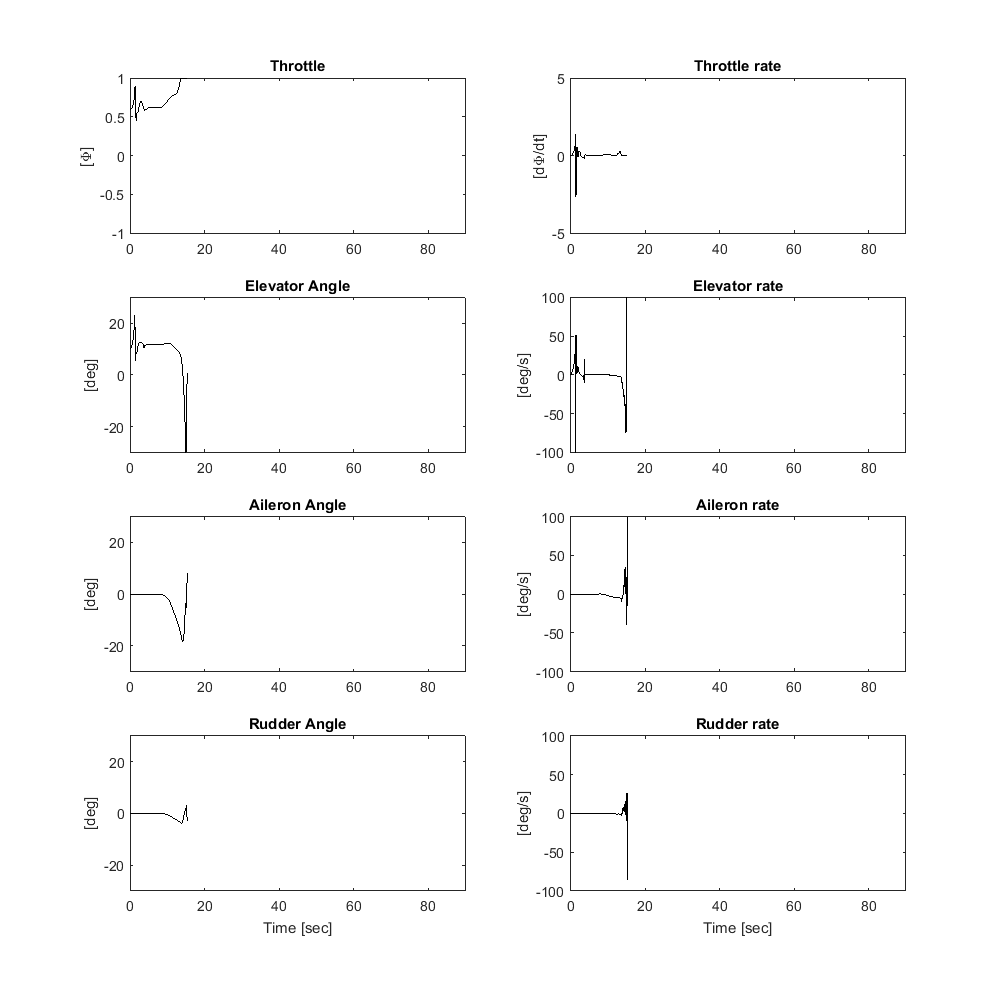
\includegraphics[width=7.5in]{\figurepath/baselineUncertainLatrControl.png}}
  \vspace{-1.0in}
  \caption{Plant control input for baseline controller applied to uncertain plant in response to a 5 degree heading turn.\label{fig.baselineUncertainLatrControl}}
\end{figure}

\newpage
\begin{figure}[H]
  \hspace{-0.5in}
  \noindent\makebox[7.5in]{%
  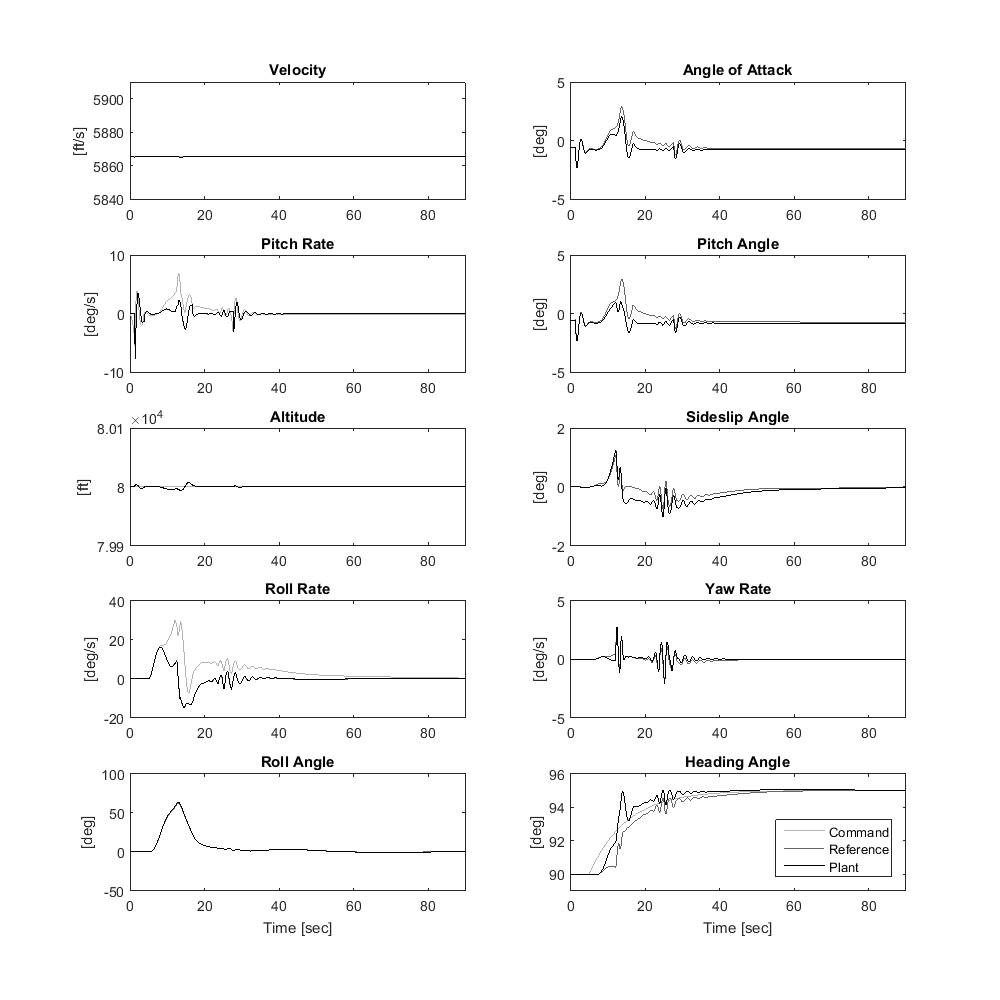
\includegraphics[width=7.5in]{\figurepath/adaptiveUncertainLatrState.png}}
  \vspace{-1.0in}
  \caption{Plant states for adaptive controller applied to uncertain plant in response to a 5 degree heading turn.\label{fig.adaptiveUncertainLatrState}}
\end{figure}

\newpage
\begin{figure}[H]
  \hspace{-0.5in}
  \noindent\makebox[7.5in]{%
  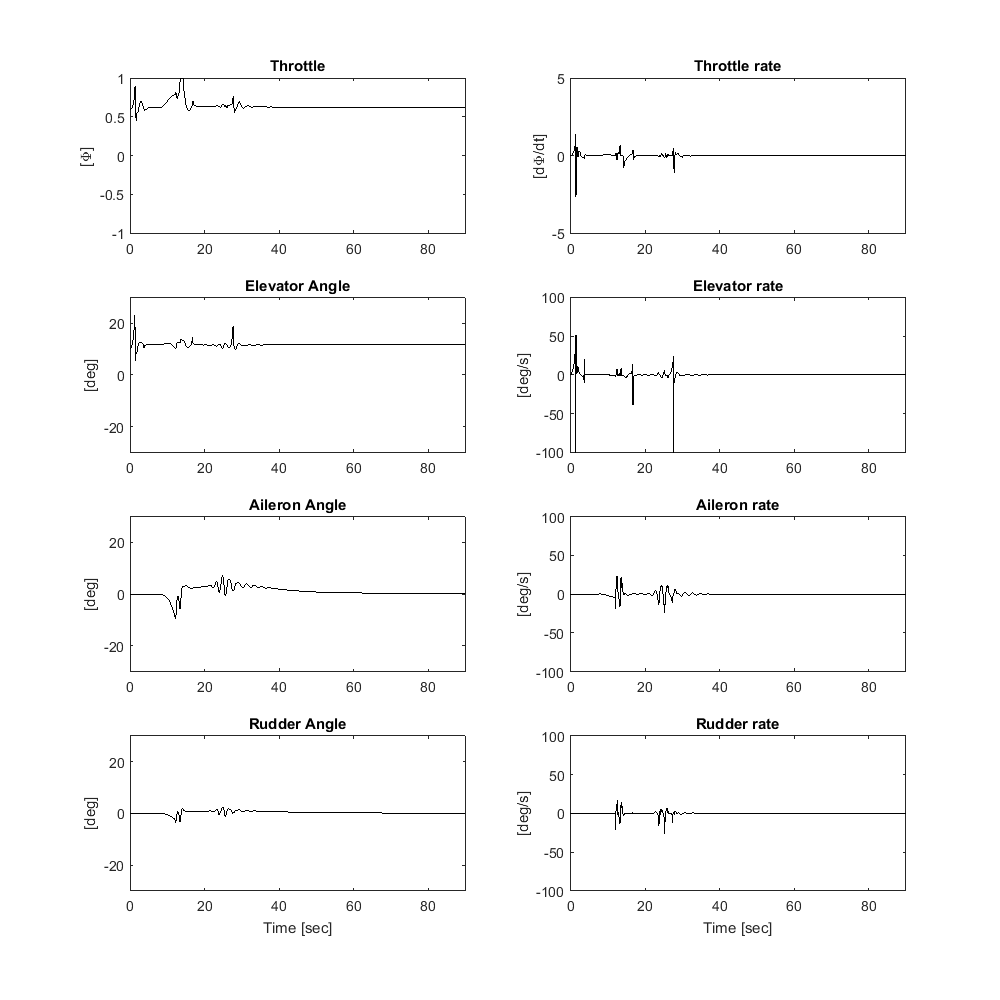
\includegraphics[width=7.5in]{\figurepath/adaptiveUncertainLatrControl.png}}
  \vspace{-1.0in}
  \caption{Plant control input for adaptive controller applied to uncertain plant in response to a 5 degree heading turn.\label{fig.adaptiveUncertainLatrControl}}
\end{figure}

\subsection{Outer-loop Response with Limiter}

The outer-loop responses in Sec.~\ref{sec.numericalExample.outerLoop} showed the ability of the combined inner and outer-loop controller to provide good command tracking of the outer-loop heading and altitude commands, while maintaining stability in the presence of uncertainty when the baseline controller could not.
However, despite stability and good command tracking performance, in Figs.~\ref{fig.adaptiveUncertainLatrState} and~\ref{fig.adaptiveUncertainLatrControl}, for example, there are significant oscillations present in the response, and large deviations in sideslip.
On the GHV such large deviations in sideslip angle would likely lead to unstart and further instability, although this phenomenon was not captured in the nonlinear GHV model used for the simulations in this thesis.
Regardless, it is beneficial to be able to suppress these large sideslip angle deviations, and ensure coordinated flight is maintained.
It is for this purposed that the limiter described in Sec.~\ref{sec.outerLoop.stateLimiting} is used.

Figs.~\ref{fig.stateLimiterState} and~\ref{fig.stateLimiterControl} show the same response as in Figs.~\ref{fig.adaptiveUncertainLatrState} and~\ref{fig.adaptiveUncertainLatrControl}, with the exception of the addition of the state limiter.
The modulation function is selected so as $\gamma=0$ for $\beta\in[-0.1,\;0.1]$ deg, and $\gamma=1$ for $\beta\notin[-0.2,\;0.2]$.
These regions, defined by the sets $\Omega_{\delta}$ and $\Omega$, are plotted in the figure.
Corollary~\ref{cor.notForcingLimiting} is easily verified, to ensure that for the given heading angle command that asymptotic tracking will be achieved.
This agrees with intuition, as it is expected that at the completion of a turn to a new heading, that the aircraft should be in coordinated flight, with zero sideslip angle.
Furthermore, by enforcing coordinated flight throughout the turn, Figs.~\ref{fig.adaptiveUncertainLatrState} and~\ref{fig.adaptiveUncertainLatrControl} show the drastically reduced oscillations observed in Figs.~\ref{fig.stateLimiterState} and~\ref{fig.stateLimiterControl}.

To further illustrate the effect that the limiter has on the inner and outer-loop commands, Fig.~\ref{fig.comparison} shows a comparison between the inner and outer-loop commands from the response without the limiter, shown in Fig.~\ref{fig.adaptiveUncertainLatrState}, to those with the limiter, shown in Fig.~\ref{fig.stateLimiterState}.
When not using the limiter, the outer-loop command is equal to the desired value, that is $z_{g,\text{cmd}}(t)=z_{g,\text{cmd}}^{\prime}(t)$, and the inner-loop input is also equal to the command value as $r(t)=r_{\text{cmd}}(t)$.
When using the limiter, the command $z_{g,\text{cmd}}(t)$ and $r(t)$ are modified from the desired or commanded values, as shown.
The limiting of both of these inner and outer-loop command signals is what is used to limit the sideslip angle, also shown in Fig.~\ref{fig.comparison}.
Because the outer-loop command $z_{g,\text{cmd}}(t)$ is used to generate the inner-loop command $r_{\text{cmd}}(t)$, the outer-loop limiting has an indirect effect on the inner-loop command.
However, the inner-loop command is further limited, resulting in $r(t)$ as shown.
It is the limiting of these commands that is responsible for the improved time response demonstrated in the simulations

From Corollary~\ref{cor.notForcingLimiting}, another situation that may be encountered, is one where for piecewise constant commands $\|z_{g,\text{cmd}}^{\prime}(t)\|_{\infty}>z_{g,\text{cmd,max}}^{\prime}$, in which case asymptotic tracking of the command is not obtained.
Consider, for example, applying the state limiter to enforce a limit on the roll angle, so as to limit the G-loading during a turn.
Figs.~\ref{fig.stateLimiterRollAngleState} and~\ref{fig.stateLimiterRollAngleControl} show the state limiter used in this way to limit the roll angle to 20 degrees.
However, by limiting the bank angle during a turn, the turn rate of the aircraft is limited.
To make large heading angle changes, large bank angles are required.
With the roll angle limiter becoming invoked simply as a result of the command, asymptotic command tracking does not follow.

\newpage
\begin{figure}[H]
  \hspace{-0.5in}
  \noindent\makebox[7.5in]{%
  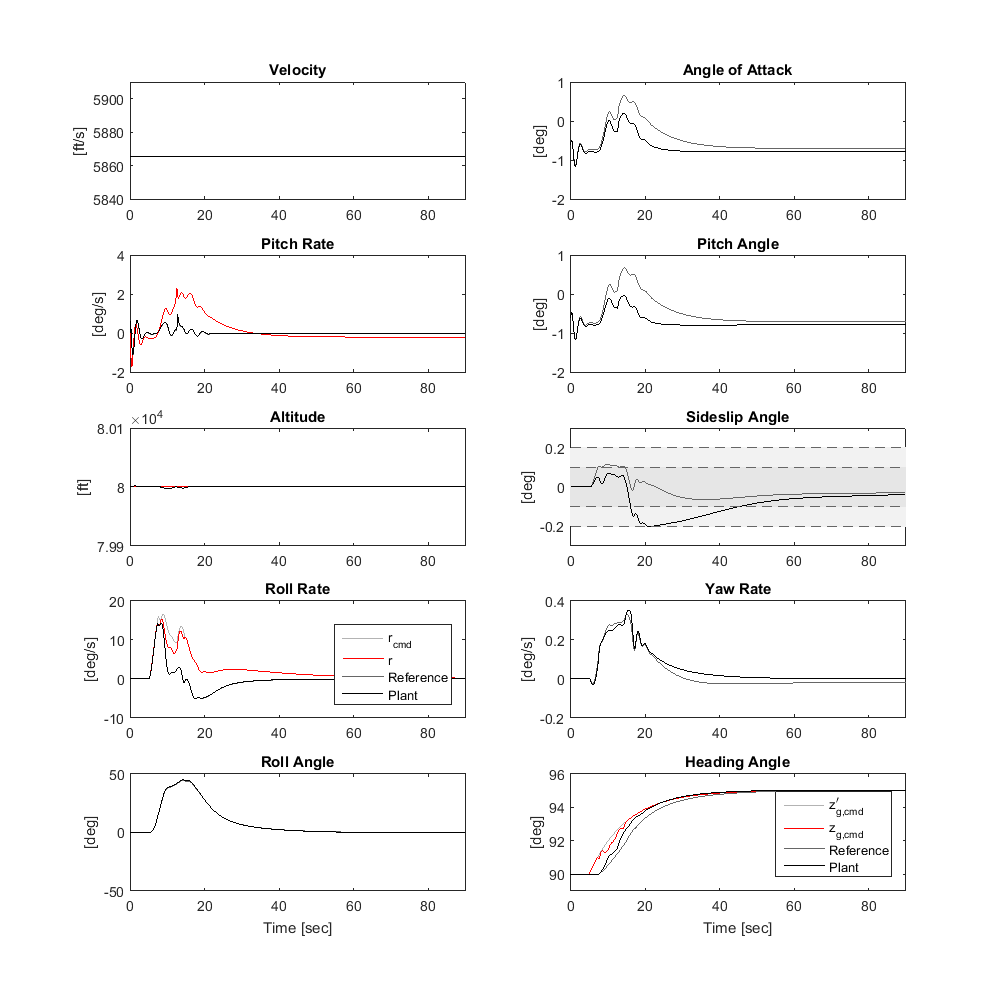
\includegraphics[width=7.5in]{\figurepath/adaptiveStateLimiterLatr2State.png}}
  \vspace{-1.0in}
  \caption{Plant states for adaptive controller applied to uncertain plant in response to a 5 degree heading turn with sideslip angle Limiter.\label{fig.stateLimiterState}}
\end{figure}

\newpage
\begin{figure}[H]
  \hspace{-0.5in}
  \noindent\makebox[7.5in]{%
  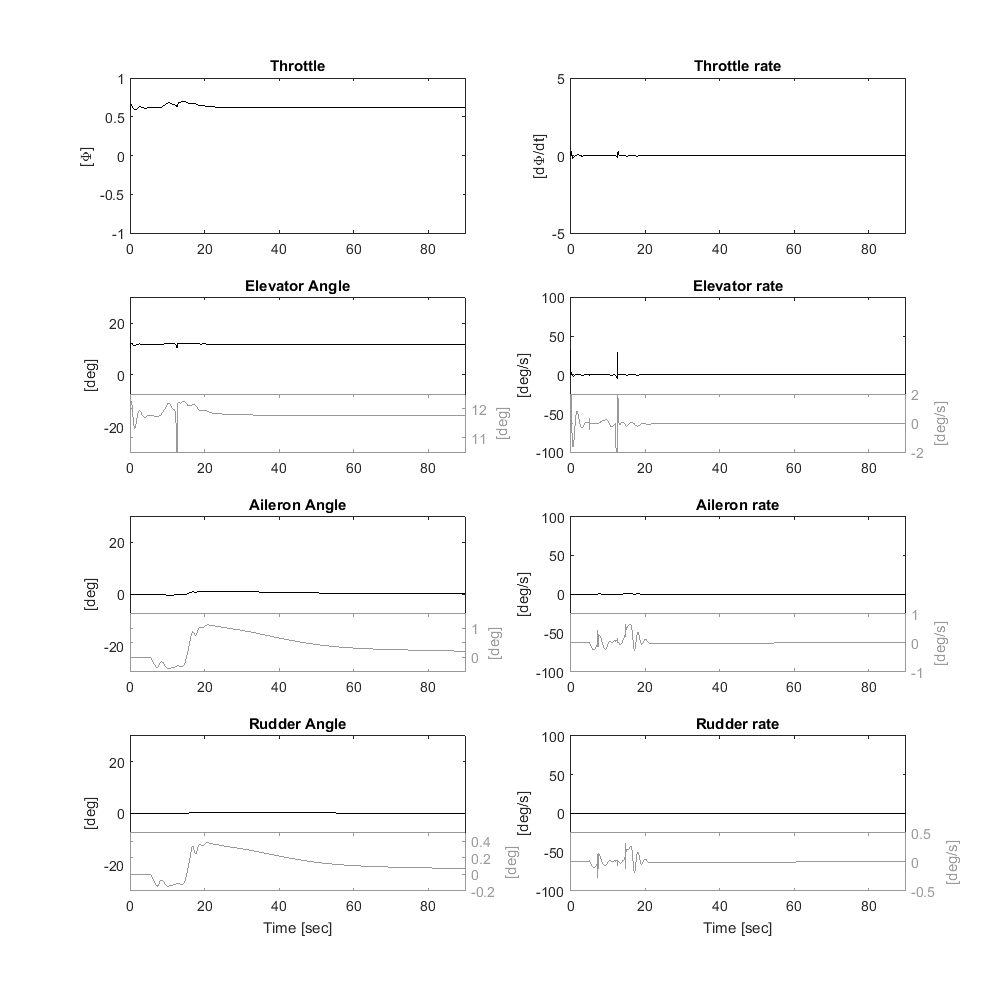
\includegraphics[width=7.5in]{\figurepath/adaptiveStateLimiterLatr2Control.png}}
  \vspace{-1.0in}
  \caption{Plant control input for adaptive controller applied to uncertain plant in response to a 5 degree heading turn with sideslip angle Limiter.\label{fig.stateLimiterControl}}
\end{figure}

\newpage
\begin{figure}[H]
  \hspace{-0.5in}
  \noindent\makebox[7.5in]{%
  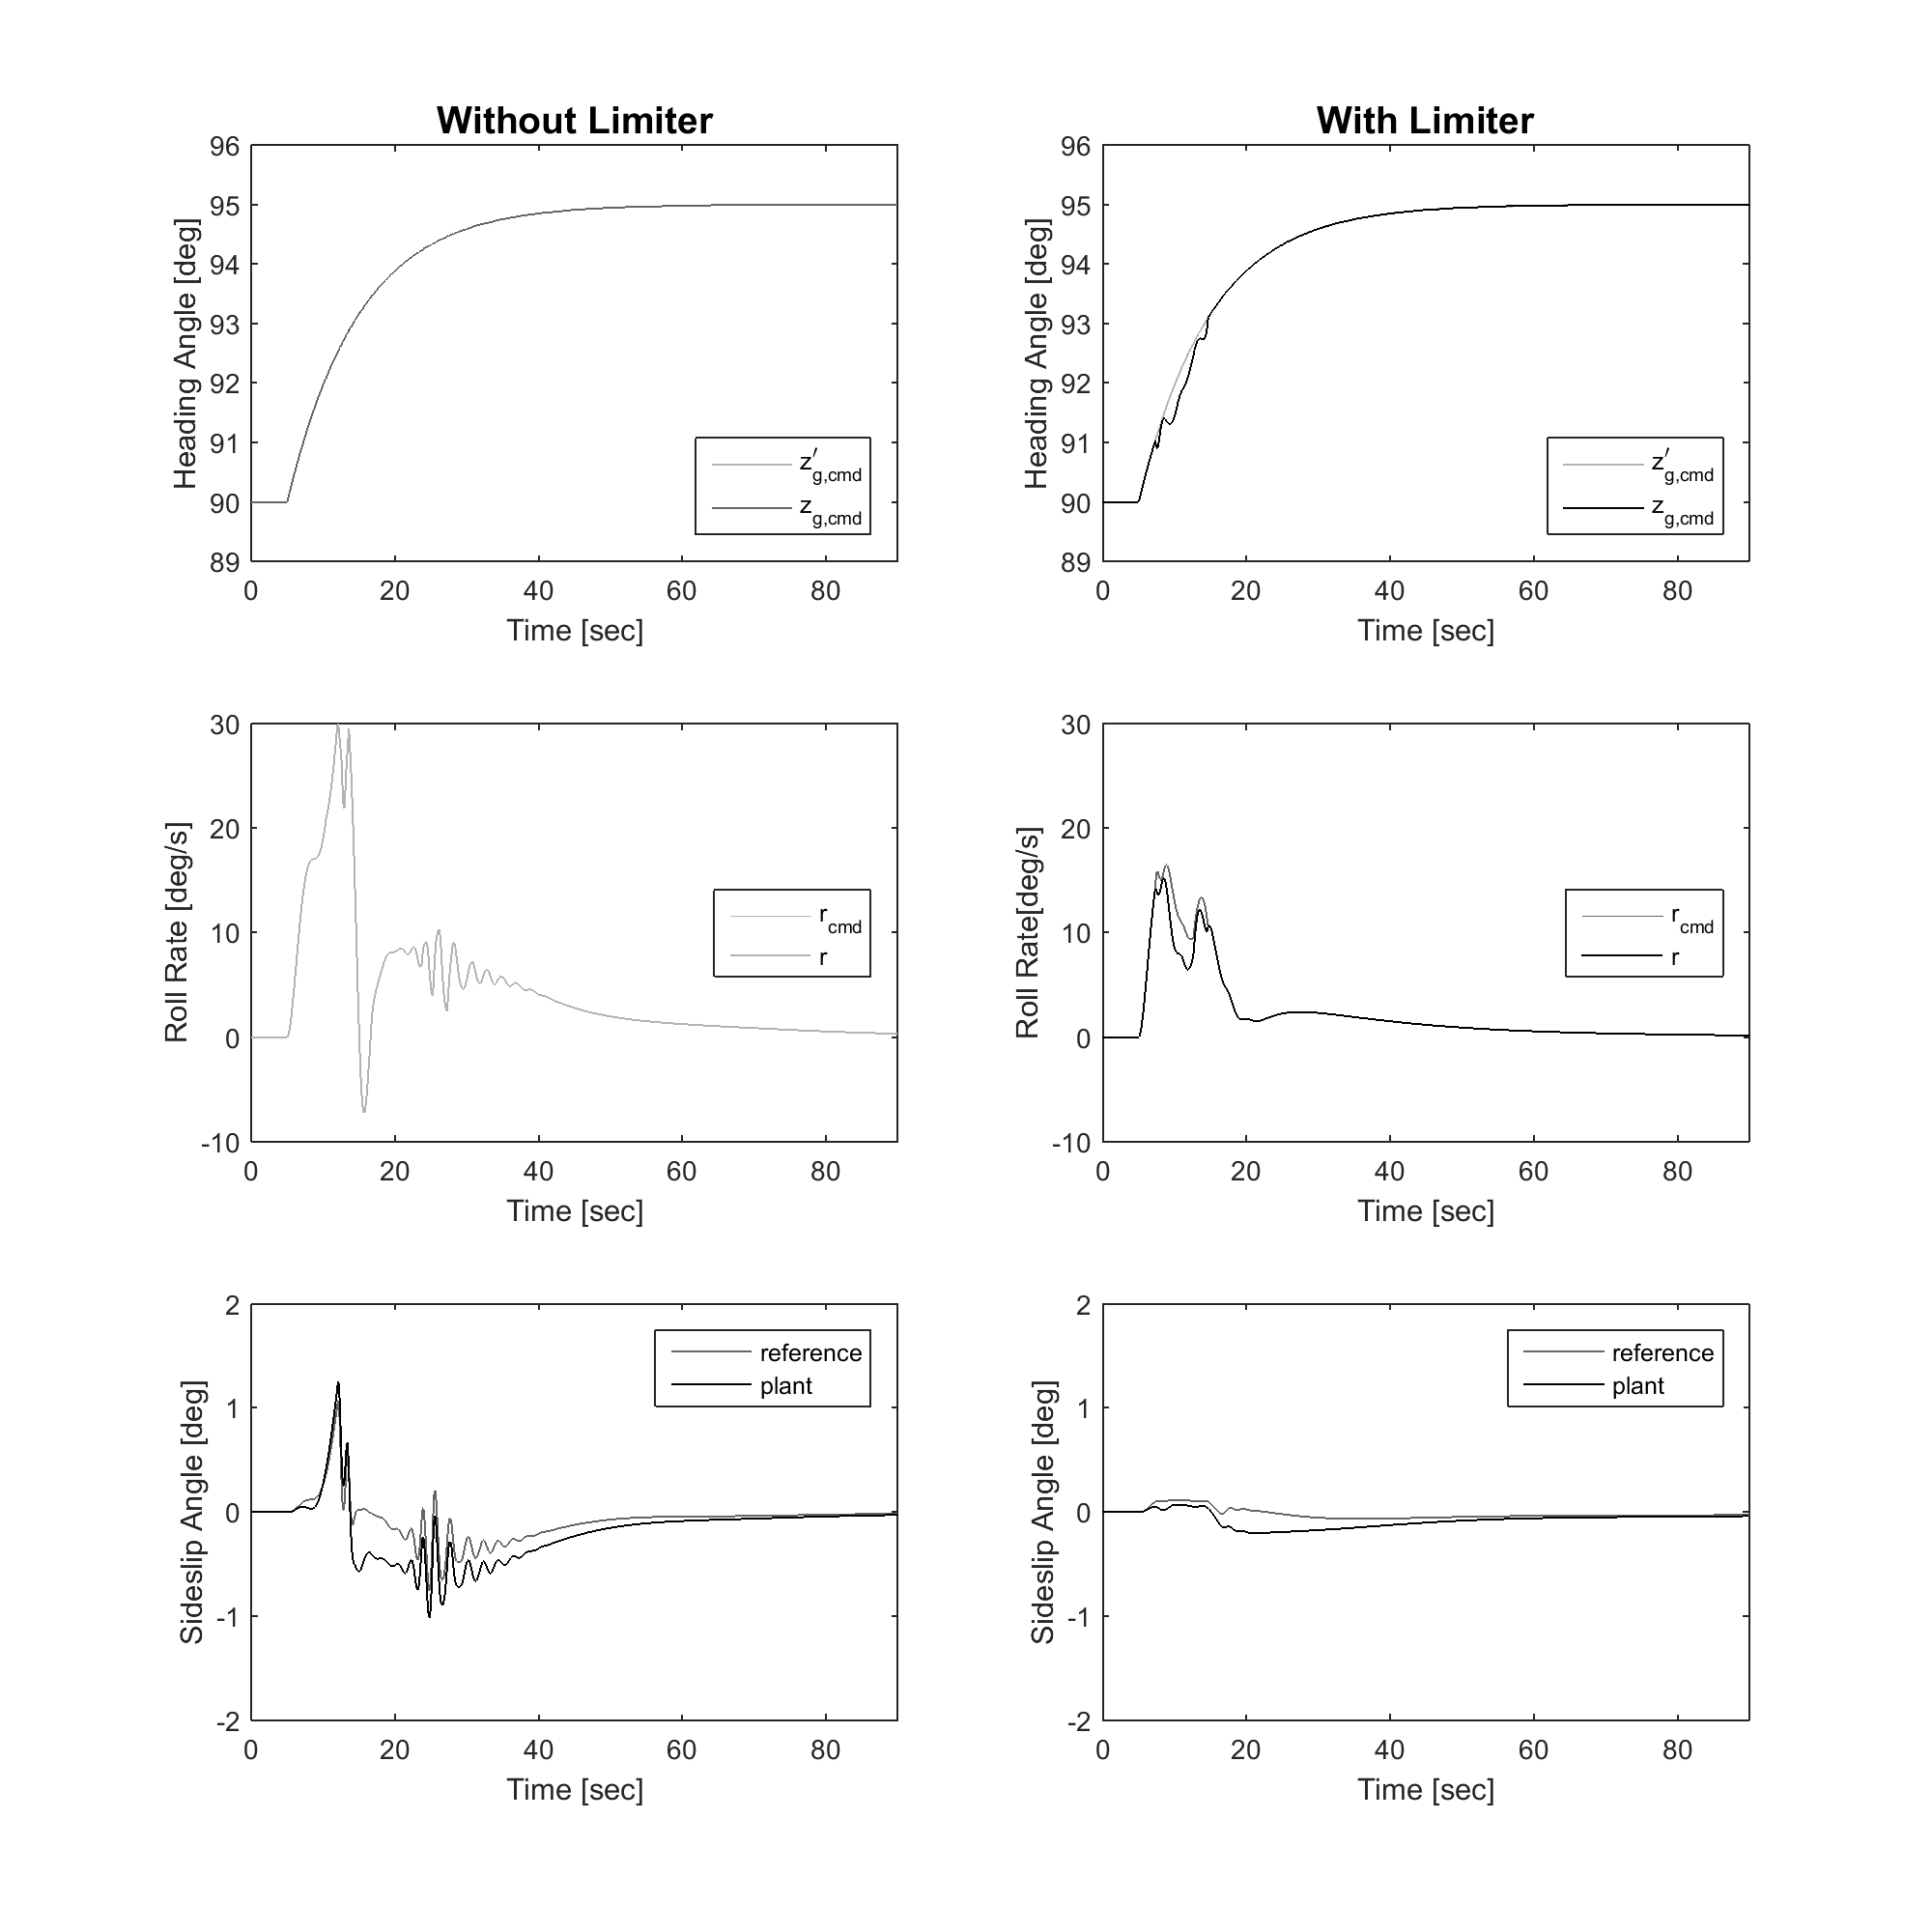
\includegraphics[width=7.5in]{\figurepath/comparison2.png}}
  \vspace{-1.0in}
  \caption{Comparison between inner and outer-loop commands when using the limiter to limit sideslip angle.\label{fig.comparison}}
\end{figure}

\newpage
\begin{figure}[H]
  \hspace{-0.5in}
  \noindent\makebox[7.5in]{%
  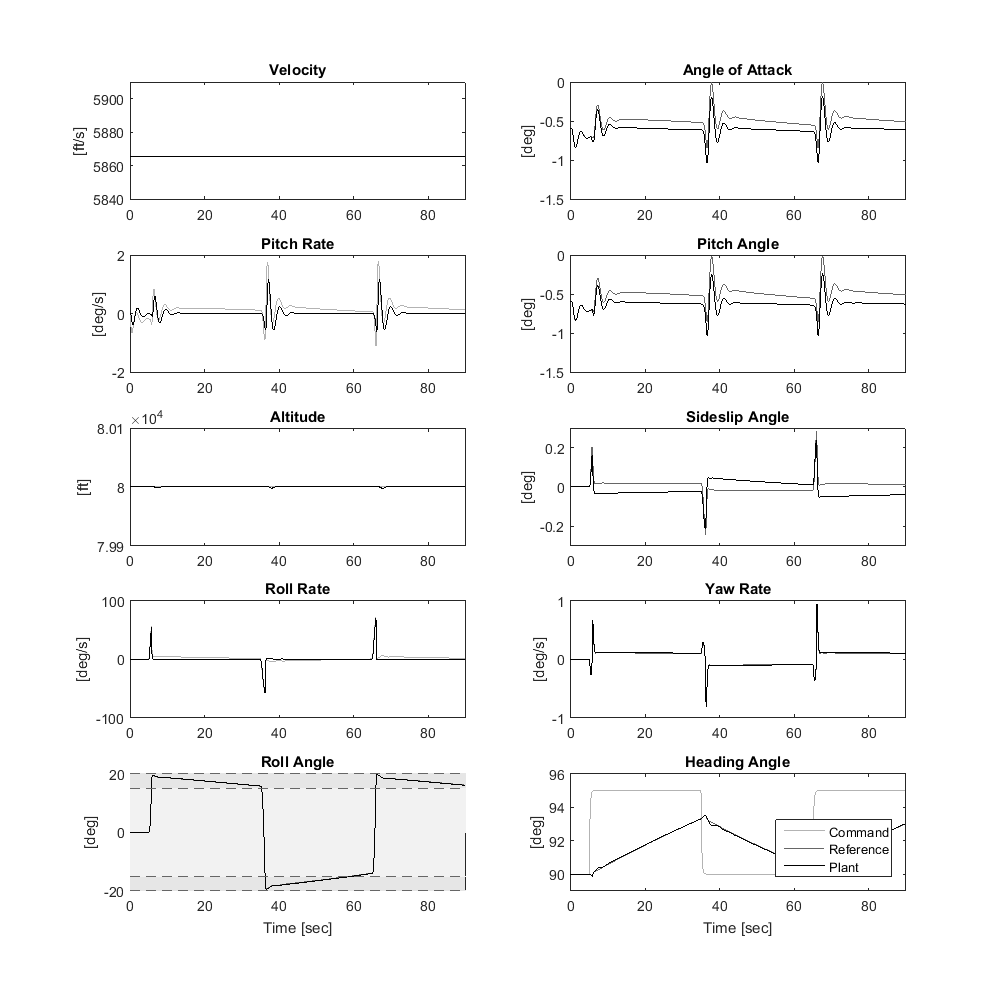
\includegraphics[width=7.5in]{\figurepath/baselineStateLimiterLatrRollAngleState.png}}
  \vspace{-1.0in}
  \caption{Plant states for adaptive controller applied to uncertain plant in response to a 5 degree heading turn with roll angle Limiter.\label{fig.stateLimiterRollAngleState}}
\end{figure}

\newpage
\begin{figure}[H]
  \hspace{-0.5in}
  \noindent\makebox[7.5in]{%
  \includegraphics[width=7.5in]{\figurepath/baselineStateLimiterLatrRollAngleControl.png}}
  \vspace{-1.0in}
  \caption{Plant control input for adaptive controller applied to uncertain plant in response to a 5 degree heading turn with roll angle Limiter.\label{fig.stateLimiterRollAngleControl}}
\end{figure}

\chapter{Conclusions and Future Work}\label{ch.conclusions}

This thesis presented the design of an adaptive controller for a class of uncertain MIMO systems.
Synthesis of the controller is completed using a sequential loop closure based procedure, where an adaptive inner-loop controller is designed first, followed by an outer-loop controller.

The inner-loop controller is capable of accommodating the uncertainty present in the plant, only requires the plant output, and provides command tracking of an inner-loop regulated output.
The controller is uses a baseline Luneberger observer based controller, which, when combined with the adaptive element provides the closed-loop reference model structure.
This thesis provided a new way of synthesizing the gain matrices required for such a controller, providing a larger set of solutions and extra degrees of freedom to tune the controller for increased performance and robustness.

The outer-loop controller generates appropriate inner-loop commands so that the outer-loop plant regulated output follows a desired command trajectory.
The outer-loop controller incorporates a state-limiter, allowing the inner and outer-loop command signals to be modified as necessary to limit the evolution of the state trajectories to within a certain prescribed region within the state space.
The outer-loop controller also uses components of a closed-loop reference model, and the resulting closed-loop system is shown to be globally stable.

This sequential loop closure based procedure to synthesize an outer-loop controller simplifies the process of designing guidance and control laws from that of designing a single higher-order controller to several lower-order controllers.
The proposed approach provides an outer-loop control design which does not require a re-design of the existing inner-loop, and guarantees global stability of the closed-loop system, and enforces desired state limits.

Finally, this adaptive controller was applied to a highly nonlinear, unstable, six degree-of-freedom Generic Hypersonic Vehicle model, which includes unmodeled actuator dynamics.
The performance of the GHV was evaluated by providing altitude and heading commands, when subject to uncertainty.
The proposed adaptive controller was shown to provide stability when the baseline could not, accommodated the desired state limits, and provided command tracking.

The control design presented in this thesis has provided a new control architecture, and a constructive procedure to synthesize the required gain matrices to provide stability and command tracking.
This procedure used to synthesize the gain matrices has provided a large set of solutions, from which the control designer can select each of the desired matrices.
This has, in practice, provided very good control designs with little effort.
However, work remains to determine methods or rules by which to select from the set of possible controller solutions ones that are more desirable than others.
This may help to ensure the control gains are minimized, to provide specific frequency domain properties for the underlying baseline controller, or minimize control effort, for example.

In addition, the state limiter presented in Section~\ref{sec.outerLoop.stateLimiting} requires further analysis.
While some qualitative analysis was done to understand how the state limiter can be used to improve the time response of a system by enforcing limits, work remains to quantify this benefit more precisely.
In particular, the state limiter introduces many additional degrees of freedom that must be fully understood in order to more successfully design and implement  the limiter on future systems.

\appendix
\chapter{Hypersonic Vehicle Numerical Simulation Data}\label{app.numericalSimulationData}

This appendix contains the numerical data for each of the three plant subsystems and the corresponding controllers that were designed for the Generic Hypersonic Vehicle in Ch.~\ref{ch.applicationHypersonic}.

\section{Velocity Subsystem}

The velocity subsystem is of the form\ \eqref{eqn.xdotpunc}.
It is a scalar system, and thus uses state feedback, and contains no outer-loop dynamics.

\subsection{Plant Data}

The open-loop plant parameters in\ \eqref{eqn.xdotpunc} are given by the following
\begin{equation*}
  A_{p} = -0.0058
  \qquad
  B_{p} = 16.7465
  \qquad
  C_{p} = 1
  \qquad
  C_{pz} = 1
  \qquad
  D_{pz} = 0
\end{equation*}

\subsection{Controller Data}

The following weighting matrices were used to compute $K_{x}$ as in Eq.\ \eqref{eqn.ubl} using the \textsc{Matlab} command \texttt{lqr}
\begin{equation*}
  \begin{aligned}
    Q_{\text{lqr}} &=
    \text{diag}\bigr(
    \begin{bmatrix}
      10 & 1
    \end{bmatrix}
    \bigr) \\
    R_{\text{lqr}} &= 10
  \end{aligned}
\end{equation*}
The following baseline control gain $K_{x}$ in Eq.\ \eqref{eqn.ubl} was computed
\begin{equation*}
  K_{x} =
  \begin{bmatrix}
    -1.0184 & 0.3162
  \end{bmatrix}^{\top}
\end{equation*}

\section{Longitudinal Subsystem}\label{sec.appendix_long}

\subsection{Plant Data}
The nominal plant matrices in the form of\ \eqref{eqn.FullLinearSystem} are given by
\begin{equation*}
  \begin{gathered}
    A_{w}=
    \begin{bmatrix}
      -0.2398 & 1 & 0 & 0 \\
      4.5689 & -0.1189 & 0 & 0 \\
      0 & 1 & 0 & 0 \\
      -5866 & 0 & 5866 & 0
    \end{bmatrix}
    \qquad
    B_{w}=
    \begin{bmatrix}
      -0.0001 \\
      -0.1856 \\
      0 \\
      0
    \end{bmatrix}
    \qquad
    C_{w} =
    \begin{bmatrix}
      0 \\
      1 \\
      0 \\
      0
    \end{bmatrix}^{\top}
  \end{gathered}
\end{equation*}
When partitioned, the inner-loop plant matrices are given by
\begin{equation*}
  \begin{gathered}
    A_{p}=
    \begin{bmatrix}
      -0.2398 & 1.0000 \\
      4.5689 & -0.1189
    \end{bmatrix}
    \qquad
    B_{p}=
    \begin{bmatrix}
      -0.0001 \\
      -0.1856
    \end{bmatrix}
    \qquad
    C_{p}=
    \begin{bmatrix}
      0 \\
      1
    \end{bmatrix}^{\top}
    \qquad
    C_{pz}=
    \begin{bmatrix}
      0 \\
      1
    \end{bmatrix}^{\top}
  \end{gathered}
\end{equation*}
with $D_{pz}=0$.
The outer-loop plant matrices are given by
\begin{equation*}
  \begin{gathered}
    A_{g} =
    \begin{bmatrix}
      0 & 0 \\
      5866 & 0 \\
    \end{bmatrix}
    \qquad
    B_{g} =
    \begin{bmatrix}
      0 & 1 \\
      -5866 & 0 \\
    \end{bmatrix}
    \qquad
    C_{g}=
    \begin{bmatrix}
      0 \\
      1
    \end{bmatrix}^{\top}
    \qquad
    C_{gz}=
    \begin{bmatrix}
      0 \\
      1
    \end{bmatrix}^{\top}
  \end{gathered}
\end{equation*}

\subsection{Controller Data}

\subsubsection{Inner-loop controller}

The following weighting matrices were used to compute $K_{x}$ as in Eq.\ \eqref{eqn.ubl} using the \textsc{Matlab} command \texttt{lqr}
\begin{equation*}
  \begin{aligned}
    Q_{\text{lqr}}&=\text{diag}\bigr(
    \begin{bmatrix}
      0 & 10 & 170
    \end{bmatrix}
    \bigr) \\
    R_{\text{lqr}}&=0.001
  \end{aligned}
\end{equation*}
The following baseline control gain $K_{x}$ in Eq.\ \eqref{eqn.ubl} was computed
\begin{equation*}
  K_{x} =
  \begin{bmatrix}
    -3.3559 & 118.5 & -412.31
  \end{bmatrix}
\end{equation*}
resulting in the following state feedback gain and phase margin
\begin{equation*}
  \begin{aligned}
    \text{GM}_{\text{sf}} &=
    \begin{bmatrix}
      -21.3 & 154.2
    \end{bmatrix}
    \quad \text{dB}\\
    \text{PM}_{\text{sf}} &=
    60
    \quad \text{deg}
  \end{aligned}
\end{equation*}
The controller was then tuned by selecting $X_{11}$, $X_{12}$, and $X_{22}$ as described in inner-loop steps~\ref{step.X22} and~\ref{step.X11} resulting in $X$ given by
\begin{equation*}
  X=
  \begin{bmatrix}
    1 & 1 \\
    1 & 318660 \\
  \end{bmatrix}
\end{equation*}
Resulting in $S_{1}$ and $L$
\begin{equation*}
  S_{1} =
  \begin{bmatrix}
    -5.0525 & 0
  \end{bmatrix}
  \qquad
  L =
  \begin{bmatrix}
    -2.6749 & 0.1586 \\
    -1979.2 & 0.0396 \\
    -0.0118 & -50527
  \end{bmatrix}
\end{equation*}
This provided the following gain and phase margin for the resulting output feedback compensator
\begin{equation*}
  \begin{aligned}
    \text{GM}_{\text{of}}
    &=
    \begin{bmatrix}
      -21.2 & 39.8
    \end{bmatrix}
    \quad \text{dB}\\
    \text{PM}_{\text{of}} &=
    59
    \quad \text{deg}
  \end{aligned}
\end{equation*}

\subsubsection{Outer-loop controller}

The forward-loop reference model was designed using integral action on the regulated output as in\ \eqref{eqn.rKbar} using the following weighting matrices
\begin{equation*}
  \begin{split}
    Q_{\text{lqr}}
    &=
    \text{diag}\bigr(
    \begin{bmatrix}
      1 & 1 & 1 & 1 & 1 & 1000
    \end{bmatrix}
    \bigr) \\
    R_{\text{lqr}}
    &=
    1000000
  \end{split}
\end{equation*}
Using the outer-loop design procedure summarized in Section~\ref{sec.outerLoopDesignProcedureSummary}, $P_{g}$ was calculated as in\ \eqref{eqn.Pg} using $P$ calculated as in\ \eqref{eqn.P} and $X_{D}$, where $P_{\Lambda}$ in\ \eqref{eqn.P}, and $X_{D}$ was selected as
\begin{equation*}
  X_{D}
  =
  \begin{bmatrix}
    1 & 3.6957e-13 \\
    3.6957e-13 & 10
  \end{bmatrix}
  \qquad
  P_{\Lambda}
  =
  \begin{bmatrix}
    0.01 & 0 \\
    0 & 1
  \end{bmatrix}
\end{equation*}
With the resulting $P_{g}$, $S_{g}=2.0319$ was determined using\ \eqref{eqn.SgCaseI}, and $L_{g}$ obtained numerically satisfying\ \eqref{eqn.condition4a}.
Finally $L_{y}$ was computed using\ \eqref{eqn.Ly} thus completing the outer-loop control design.
\begin{equation*}
  \begin{gathered}
    P_{g} =
    \begin{bmatrix}
      10 & 5.1073e-15 \\
      5.1073e-15 & 0.00041288
    \end{bmatrix}
    \qquad
    L_{g} =
    \begin{bmatrix}
      -0.20218 \\
      -82.576
    \end{bmatrix}
    \qquad
    L_{y} =
    \begin{bmatrix}
      -1 & 2.5135e-12 \\
      4.0446 & -4921.4
    \end{bmatrix}
  \end{gathered}
\end{equation*}

\section{Lateral Subsystem}\label{sec.appendix_latr}

\subsection{Plant Data}

The nominal plant matrices in the form of\ \eqref{eqn.FullLinearSystem} are given by
\begin{equation*}
  \begin{split}
    A_{w} &=
    \begin{bmatrix}
      -0.0697 & -0.0104 & -1.0000 & 0.0053512 & 1e-12 \\
      -1336.7 & -2.026 & -0.0075 & 0 & 0 \\
      2.0689 & -0.0015 & -0.0531 & 0 & 0 \\
      -0.0002 & 0.8535 & -0.0088 & -3.0021e-06 & 6.2245e-05 \\
      2.8915e-06 & 0 & 1.0001 & 2.9365e-08 & -8.6563e-07 \\
    \end{bmatrix} \\
    \qquad
    B_{w} &=
    \begin{bmatrix}
      0 & 0.0002 \\
      -8.0424 & 10.325 \\
      0.0317 & -0.2848 \\
      0 & 0 \\
      0 & 0 \\
    \end{bmatrix}
    \qquad
    C_{w} =
    \begin{bmatrix}
      0 & 1 & 0 & 0 & 0 \\
      0 & 0 & 1 & 0 & 0 \\
      0 & 0 & 0 & 0 & 1 \\
    \end{bmatrix} \\
  \end{split}
\end{equation*}
When partitioned, the inner-loop plant matrices are given by
\begin{equation*}
  \begin{gathered}
    A_{p}=
    \begin{bmatrix}
      -0.0697 & -0.0104 & -1.0000 \\
      -1336.7 & -2.026 & -0.0075 \\
      2.0689 & -0.0015 & -0.0531 \\
    \end{bmatrix}
    \hspace{0.5in}
    B_{p}=
    \begin{bmatrix}
      0 & 0.0002 \\
      -8.0424 & 10.325 \\
      0.0317 & -0.2848 \\
    \end{bmatrix} \\
    C_{p}=
    \begin{bmatrix}
      0 & 1 & 0 \\
      0 & 0 & 1 \\
    \end{bmatrix}
    \qquad
    C_{pz}=
    \begin{bmatrix}
      0 & 0 & 1
    \end{bmatrix}
    \qquad
    D_{pz} =
    \begin{bmatrix}
      0 & 0
    \end{bmatrix}
  \end{gathered}
\end{equation*}
The outer-loop plant matrices are given by
\begin{equation*}
  \begin{gathered}
    A_{g} =
    \begin{bmatrix}
      -3.0021e-06 & 6.2245e-05 \\
      2.9365e-08 & -8.6563e-07 \\
    \end{bmatrix}
    \qquad
    B_{g} =
    \begin{bmatrix}
      -0.0002 & 0.8535 & -0.0088 \\
      2.8915e-06 & 0 & 1.0001 \\
    \end{bmatrix} \\
    C_{g} =
    \begin{bmatrix}
      0 & 1
    \end{bmatrix}
    \qquad
    C_{gz} =
    \begin{bmatrix}
      0 & 1
    \end{bmatrix}
  \end{gathered}
\end{equation*}

\subsection{Controller Data}

\subsubsection{Inner-loop controller}

The following weighting matrices were used to compute $K_{x}$ as in Eq.\ \eqref{eqn.ubl} using the \textsc{Matlab} command \texttt{lqr()}
\begin{equation*}
  \begin{aligned}
    Q_{\text{lqr}} &=
    \text{diag}\bigr(
    \begin{bmatrix}
      1000 & 0 & 0 & 1000
    \end{bmatrix}
    \bigr) \\
    R_{\text{lqr}}
    &=
    \text{diag}\bigr(
    \begin{bmatrix}
      0.01 & 0.01
    \end{bmatrix}
    \bigr)
  \end{aligned}
\end{equation*}
The baseline control gain $K_{x}$ in Eq.\ \eqref{eqn.ubl} was computed
\begin{equation*}
  K_{x} =
  \begin{bmatrix}
    -281.19 & 7.2309 & 50.495 & -265.57 \\
    -288.63 & -3.4406 & 75.18 & 171.68
  \end{bmatrix}^{\top}
 \end{equation*}
which resulting in the following state feedback gain and phase margin
\begin{align*}
  \text{GM}_{\text{sf}} &=
  \begin{bmatrix}
    -11.2 & 276.4
  \end{bmatrix}
  \quad \text{dB} \\
  \text{PM}_{\text{sf}} &=
  60
  \quad \text{deg}
\end{align*}
The controller was then tuned by selecting $X_{11}$, $X_{12}$, and $X_{22}$ as described in inner-loop steps~\ref{step.X22} and~\ref{step.X11} resulting in $X$ given by
\begin{equation*}
  X=
  \begin{bmatrix}
    1 & 1 \\
    1 & 2.5426e+05
  \end{bmatrix}
\end{equation*}
The resulting $S_{1}$ and $L$ were calculated
\begin{equation*}
  S_{1} =
  \begin{bmatrix}
    -0.1638 & -5.8866 & 0 \\
    -0.0581 & -8.6832 & 0
  \end{bmatrix}
  \qquad
  L =
  \begin{bmatrix}
    -0.1196 & 1.0446 & -0.0179 \\
    -10556 & 140.29 & 0.0098 \\
    140.33 & -43.212 & 0 \\
    0.9996 & -0.0124 & -4552.4 \\
  \end{bmatrix}
\end{equation*}
This provided the following gain and phase margin for the resulting output feedback compensator
\begin{align*}
  \text{GM}_{\text{of}} &=
  \begin{bmatrix}
    -10.0 & 16.4
  \end{bmatrix}
  \quad \text{dB}\\
  \text{PM}_{\text{of}} &=
  50.3
  \quad \text{deg}
\end{align*}

\subsubsection{Outer-loop controller}

The forward-loop reference model was designed using integral action on the regulated output as in\ \eqref{eqn.rKbar} using the following weighting matrices
\begin{equation*}
  \begin{split}
    Q_{\text{lqr}}
    &=
    \text{diag}\bigr(
    \begin{bmatrix}
      20 & 1 & 0 & 0 & 0 & 0 & 1000
    \end{bmatrix}
    \bigr) \\
    R_{\text{lqr}}
    &=
    0.1
  \end{split}
\end{equation*}
Using the outer-loop design procedure summarized in Section~\ref{sec.outerLoopDesignProcedureSummary}, $P_{g}$ was calculated as in\ \eqref{eqn.Pg} using $P$ calculated as in\ \eqref{eqn.P} and $X_{D}$, where $P_{\Lambda}$ in\ \eqref{eqn.P}, and $X_{D}$ was selected as
\begin{equation*}
  X_{D}
  =
  \begin{bmatrix}
    10.408 & -6.3861 \\
    -6.3861 & 100
  \end{bmatrix}
  \qquad
  P_{\Lambda}
  =
  \begin{bmatrix}
    1000 & 0 \\
    0 & 1
  \end{bmatrix}
\end{equation*}
With the resulting $P_{g}$, $S_{g}=-15.474$ was determined using\ \eqref{eqn.SgCaseI}, and $L_{g}$ obtained numerically satisfying\ \eqref{eqn.condition4a}.
Finally $L_{y}$ was computed using\ \eqref{eqn.Ly} thus completing the outer-loop control design.
\begin{equation*}
  \begin{gathered}
    P_{g} =
    \begin{bmatrix}
      100 & -23051 \\
      -23051 & 3.403e+07 \\
    \end{bmatrix}
    \qquad
    L_{g} =
    \begin{bmatrix}
      -0.0004854 \\
      -5.0844e-07
    \end{bmatrix} \\
    L_{y} =
    \begin{bmatrix}
      -0.85355 & -0.0021509 & 0.00012421 \\
      -9.8889e-13 & -1 & 5.3885e-07
    \end{bmatrix}
  \end{gathered}
\end{equation*}

\chapter{Preliminaries}\label{app.preliminaries}

\paragraph{Annihilators} 
Given a matrix $B$, the matrix $B^{\perp}$ is a basis for the orthogonal complement, or annihilator of $B$.
That is $B^{\perp}$ satisfies $B^{\perp\top}B=0$.
In addition, in this thesis, this notation is used to indicate that this basis be selected to be orthonormal.

\paragraph{Inverses}
Given a full rank matrix $B\in\mathbb{R}^{n\times m}$, when $B$ is square, that is $n=m$, the inverse of $B$ is written $B^{-1}$ and satisfies $BB^{-1}=I$.
When $B$ is tall, that is $n>m$, $B$ has a left inverse $B^{-1_{\text{left}}}\in\mathbb{R}^{m\times n}$ which satisfies
\begin{equation}
  B^{-1_{\text{left}}}B = I_{m\times m}
\end{equation}
where $B^{-1_{\text{left}}}$ is given by
\begin{equation}
  B^{-1_{\text{left}}} = (B^{\top}B)^{-1}B^{\top}
\end{equation}
When $B$ is wide, that is $n<m$, $B$ has a right inverse $B^{-1_{\text{right}}}\in\mathbb{R}^{m\times n}$ which satisfies
\begin{equation}
  BB^{-1_{\text{right}}} = I_{n\times n}
\end{equation}
where $B^{-1_{\text{right}}}$ is given by
\begin{equation}
  B^{-1_{\text{right}}} = B^{\top}(BB^{\top})^{-1}
\end{equation}

The following well-known lemma gives necessary and sufficient conditions to ensure that the system $(A,B,C,0)$ is strictly positive real (SPR).

\begin{lem-dan}[(Kalman-Yakubovic)]\label{lem.KY}
  Given the strictly proper transfer matrix $G(s)$ with stabilizable and detectable realization $(A,B,C,0)$, where $A\in\mathbb{R}^{n\times n}$ is asymptotically stable, $B\in\mathbb{R}^{n\times m}$ and $C\in\mathbb{R}^{m\times n}$, then $G(s)$ is SPR if and only if there exists a $P=P^{\top}>0$ such that
  \begin{align}
    \label{eqn.lyapal2}
    A^{\top}P+PA&<0 \\
    \label{eqn.pbc}
    PB&=C^{\top}
  \end{align} 
\end{lem-dan}

\begin{proof-dan}
  The proof can be found in Reference\ \cite{narendra.frequency.1973}.
\end{proof-dan}

\begin{cor-dan}
  There exists a matrix $P=P^{\top}>0$ that satisfies\ \eqref{eqn.pbc} if and only if 
  \begin{equation}
    \label{eqn.cbeqcbt}
    CB=(CB)^{\top}>0
  \end{equation}
  Furthermore, when\ \eqref{eqn.cbeqcbt} holds, all solutions of\ \eqref{eqn.pbc} are given by
  \begin{equation}
    \label{eqn.Psolutions}
    P=C^{\top}(CB)^{-\top}C+B^{\perp}XB^{\perp\top}
  \end{equation}
  where $X=X^{\top}>0$ is arbitrary and $B^{\perp}\in\mathbb{R}^{n\times(n-m)}$.
\end{cor-dan}

\begin{proof-dan}
  The proof can be found in Reference\ \cite{huang.designspr.1999}.
\end{proof-dan}

\begin{lem-dan}[(Matrix Elimination)]\label{lem.elimination}
  Given 
  \begin{equation}
    \label{eqn:ineqprove}
    G+C^{\top}L^{\top}P+PLC<0
  \end{equation}
  where $G\in\mathbb{R}^{n\times n}$, $C\in\mathbb{R}^{p\times n}$, and $P=P^{\top}\in\mathbb{R}^{n\times n}$ is full rank, an $L\in\mathbb{R}^{n\times p}$ exists which satisfies\ \eqref{eqn:ineqprove} if and only if the following inequality holds
  \begin{equation*}
    C^{\top\perp\top}GC^{\top\perp}<0
  \end{equation*}
  where $C^{\top\perp}\in\mathbb{R}^{n\times(n-p)}$ satisfies $CC^{\top\perp}=0$.
\end{lem-dan}

\begin{proof-dan}
  The proof can be found in Reference\ \cite{boyd.lmibook.1994}.
\end{proof-dan}

\chapter{Proofs}\label{app.proofs}

\begin{lem-dan}
  Theorem~\ref{thm.existenceOuterLoop} holds for systems where $n-p\geq n_{g}$ if the following conditions are satisfied
  \begin{align}
    \label{eqn.PiAtallCond1}
    \Pi_{B}^{\top}\Pi_{A}^{-1_{\text{\rm{left}}}}\Pi_{C} &=
    (\Pi_{B}^{\top}\Pi_{A}^{-1_{\text{\rm{left}}}}\Pi_{C})^{\top} \\
    \label{eqn.PiAtallCond2}
    U_{2}^{\top}\Pi_{C}^{\top}\Pi_{A}^{-\top_{\text{\rm{left}}}} &= 0 \\
    \label{eqn.PiAtallCond3}
    U_{1}^{\top}\Pi_{C}^{\top}\Pi_{A}^{-\top_{\text{\rm{left}}}}V_{1}\Sigma &>0
  \end{align}
  where $U_{1}$, $V_{1}$, and $\Sigma$ are found by performing a singular value decomposition on $\Pi_{B}^{\top}$ as described in\ \cite{hua.symmetric.1990}, and for the resulting $P_{g}$ to also satisfy\ \eqref{eqn.condition4bCaseI} as required, the following inequality must hold.
  \begin{equation}
    \label{eqn.PiAtallCond4}
    \Pi_{B}^{\top}A_{g}^{\top}\Pi_{A}^{-1_{\text{\rm{left}}}}\Pi_{C} +
    (\Pi_{B}^{\top}A_{g}^{\top}\Pi_{A}^{-1_{\text{\rm{left}}}}\Pi_{C})^{\top} <0
  \end{equation}
  If these conditions are satisfied, $P_{g}$ can be found as follows
  \begin{equation*}
    P_{g}
    =
    A^{-1_{\text{\rm{right}}}}B+(I-A^{-1_{\text{\rm{right}}}}A)(A^{-1_{\text{\rm{right}}}}B)^{\top}+(I-A^{-1_{\text{\rm{right}}}}A)B^{\top}(BA^{\top})B(I-A^{-1_{\text{\rm{right}}}}A)+V_{2}GV_{2}^{\top}
  \end{equation*}
  where $V_{2}$ is found by performing a singular value decomposition on $\Pi_{B}^{\top}$ as described in\ \cite{hua.symmetric.1990}, $G=G^{\top}>0$ is arbitrary, and $A$ and $B$ are given by the following
  \begin{align*}
    A &= \Pi_{B}^{\top} \\
    B &= (\Pi_{A}^{-1_{\text{\rm{left}}}}\Pi_{C})^{\top}
  \end{align*}
\end{lem-dan}

\begin{proof-dan}
  In this case, symmetric solutions to the matrix equation $\Pi_{A}P_{g}\Pi_{B}=\Pi_{C}$ must be found, where now $\Pi_{A}$ is no longer wide; it will either be square or tall.
  The matrix $\Pi_{B}$ is always tall.
  In this case the equation can be rearranged using a left inverse to obtain
  \begin{equation}
    \label{eqn.appPgPiBstuff}
    P_{g}\Pi_{B} = \Pi_{A}^{-1_{\text{\rm{left}}}}\Pi_{C}
  \end{equation}
  Taking the transpose of both sides of\ \eqref{eqn.appPgPiBstuff} gives
  \begin{equation}
    \label{eqn.appPgPiBstuff2}
    \Pi_{B}^{\top}P_{g} = \Pi_{C}^{\top}\Pi_{A}^{-\top_{\text{\rm{left}}}}
  \end{equation}
  Symmetric positive definite solutions $P_{g}=P_{g}^{\top}$ to\ \eqref{eqn.appPgPiBstuff2} are given in\ \cite{hua.symmetric.1990}.
  Satisfying the additional inequality\ \eqref{eqn.condition4b} required for Theorem~\ref{thm.existenceOuterLoop} to hold, is equivalent to the inequality\ \eqref{eqn.condition4bCaseI} using the expression for $\Pi_{B}$.
  Substituting\ \eqref{eqn.appPgPiBstuff} into\ \eqref{eqn.condition4bCaseI} gives the inequality in\ \eqref{eqn.PiAtallCond4}.
  Whether or not a given plant satisfies these conditions can be easily verified by substituting the expressions for $\Pi_{A}$, $\Pi_{B}$, and $\Pi_{C}$ from\ \eqref{eqn.AXBandCCaseI} into\ \eqref{eqn.PiAtallCond1},\ \eqref{eqn.PiAtallCond2},\ \eqref{eqn.PiAtallCond3}, and\ \eqref{eqn.PiAtallCond4}.
  Thus, the conditions in this lemma can be verified given a plant to determine the existence of the outer-loop controller, and provides the solution $P_{g}$ necessary.
\end{proof-dan}

\begin{lem-dan}
  The third conditions from\ \eqref{eqn.firstColumnOfPinv} and\ \eqref{eqn.secondColumnOfPinv}, given below, hold for matrices $\Pi_{A}$, $\Pi_{B}$, $P_{A}$, $P_{B}$, $P_{N}$ given in Chapter~\ref{ch.outerLoop}.
  \begin{align}
    \tag{\ref{eqn.firstColumnOfPinv}}
    P_{N}
    \begin{bmatrix}
      \Pi_{A}^{\top} & \Pi_{B}
    \end{bmatrix}^{\perp\top}
    \Pi_{B}^{\perp}\bigr(P_{A}\Pi_{A}\Pi_{B}^{\perp}\bigr)^{-1_{\text{\rm{right}}}}
    &= 0 \\
    \tag{\ref{eqn.secondColumnOfPinv}}
    P_{N}
    \begin{bmatrix}
      \Pi_{A}^{\top} & \Pi_{B}
    \end{bmatrix}^{\perp\top}
    \Pi_{A}^{\top\perp}\bigr(P_{B}\Pi_{B}^{\top}\Pi_{A}^{\top\perp}\bigr)^{-1_{\text{\rm{right}}}}
    &= 0
  \end{align}
\end{lem-dan}

\begin{proof-dan}
  Writing out the right inverse,\ \eqref{eqn.firstColumnOfPinv} and\ \eqref{eqn.secondColumnOfPinv} can be written as
  \begin{align*}
    P_{N}
    \begin{bmatrix}
      \Pi_{A}^{\top} & \Pi_{B}
    \end{bmatrix}^{\perp\top}
    \Pi_{B}^{\perp}
    (P_{A}\Pi_{A}\Pi_{B}^{\perp})^{\top}
    \bigr(
    (P_{A}\Pi_{A}\Pi_{B}^{\perp})
    (P_{A}\Pi_{A}\Pi_{B}^{\perp})^{\top}
    \bigr)^{-1}
    &= 0 \\
    P_{N}
    \begin{bmatrix}
      \Pi_{A}^{\top} & \Pi_{B}
    \end{bmatrix}^{\perp\top}
    \Pi_{A}^{\top\perp}
    (P_{B}\Pi_{B}^{\top}\Pi_{A}^{\top\perp})^{\top}
    \bigr(
    (P_{B}\Pi_{B}^{\top}\Pi_{A}^{\top\perp})
    (P_{B}\Pi_{B}^{\top}\Pi_{A}^{\top\perp})^{\top}
    \bigr)^{-1}
    &= 0
  \end{align*}
  Which is equivalent to satisfying
  \begin{align*}
    \begin{bmatrix}
      \Pi_{A}^{\top} & \Pi_{B}
    \end{bmatrix}^{\perp\top}
    \Pi_{B}^{\perp}
    (P_{A}\Pi_{A}\Pi_{B}^{\perp})^{\top}
    &= 0 \\
    \begin{bmatrix}
      \Pi_{A}^{\top} & \Pi_{B}
    \end{bmatrix}^{\perp\top}
    \Pi_{A}^{\top\perp}
    (P_{B}\Pi_{B}^{\top}\Pi_{A}^{\top\perp})^{\top}
    &= 0
  \end{align*}
  which in turn is equivalent to satisfying
  \begin{align*}
    \begin{bmatrix}
      \Pi_{A}^{\top} & \Pi_{B}
    \end{bmatrix}^{\perp\top}
    \Pi_{B}^{\perp}\Pi_{B}^{\perp\top}\Pi_{A}^{\top}
    &= 0 \\
    \begin{bmatrix}
      \Pi_{A}^{\top} & \Pi_{B}
    \end{bmatrix}^{\perp\top}
    \Pi_{A}^{\top\perp}\Pi_{A}^{\top\perp\top}\Pi_{B}
    &= 0
  \end{align*}
  Satisfying these two conditions is equivalent to showing
  \begin{align}
    \label{eqn.bunchPisA}
    \Pi_{B}^{\perp}\Pi_{B}^{\perp\top}\Pi_{A}^{\top}
    &=
    \begin{bmatrix}
      \Pi_{A}^{\top} & \Pi_{B}
    \end{bmatrix}K_{1} \\
    \label{eqn.bunchPisB}
    \Pi_{A}^{\top\perp}\Pi_{A}^{\top\perp\top}\Pi_{B}
    &=
    \begin{bmatrix}
      \Pi_{A}^{\top} & \Pi_{B}
    \end{bmatrix}K_{2}
  \end{align}
  where $K_{1}\in\mathbb{R}^{(n-p)+(n_{g}-p_{g})\times n-p}$ and $K_{2}\in\mathbb{R}^{(n-p)+(n_{g}-p_{g})\times n_{g}-p_{g}}$.
  We continue the sketch of the proof for\ \eqref{eqn.bunchPisA}; the same arguments apply for showing\ \eqref{eqn.bunchPisB}.
  The matrix $\Pi_{B}^{\perp\top}\Pi_{A}^{\top}$ are the projections of the columns of $\Pi_{A}^{\top}$ into the each of the orthogonal vectors of unit length which form the basis for the nullspace of $\Pi_{B}$.
  Then multiplying these quantities by $\Pi_{B}^{\perp}$ gives the vectors that are exactly the columns of $\Pi_{A}^{\top}$ projected into the nullspace of $\Pi_{B}$.
  Such a projection can be exactly represented by the right-hand-side of\ \eqref{eqn.bunchPisA}.
  That is, these projections can be obtained by scaling the columns of $\Pi_{A}^{\top}$ and subtracting off the components that are in the $\Pi_{B}$ directions.
\end{proof-dan}

\begin{lem-dan}
  Satisfying\ \eqref{eqn.Pbar21XD12lyapInequality} is independent of the selection of the matrices $P_{A}$ and $P_{B}$.
\end{lem-dan}

\begin{proof-dan}
  As $P_{B}$ in\ \eqref{eqn.Pbar21XD12lyapInequality} is full rank, it does not impact the satisfaction of the inequality.
  Thus, satisfying\eqref{eqn.Pbar21XD12lyapInequality} is equivalent to satisfying
  \begin{equation}
    \label{eqn.Pbar21XD12lyapInequality2}
    \begin{split}
      &
      \Pi_{B}^{\top}A_{g}^{\top}\Pi_{B}^{\perp}
      \bigr(P_{A}\Pi_{A}\Pi_{B}^{\perp}\bigr)^{-1_{\text{\rm{right}}}}
      P_{A}\Pi_{C}  \\
      & \qquad
      +
      \bigr(
      \Pi_{B}^{\top}A_{g}^{\top}\Pi_{B}^{\perp}
      \bigr(P_{A}\Pi_{A}\Pi_{B}^{\perp}\bigr)^{-1_{\text{\rm{right}}}}
      P_{A}\Pi_{C}
      \bigr)^{\top}
      <0
    \end{split}
  \end{equation}
  To examine how $P_{A}$ cancels the out from\ \eqref{eqn.Pbar21XD12lyapInequality2}, the inverse $\bigr(P_{A}\Pi_{A}\Pi_{B}^{\perp}\bigr)^{-1_{\text{\rm{right}}}}$ term is examined.
  The right inverse is given by
  \begin{equation*}
    \begin{split}
      \bigr(P_{A}\Pi_{A}\Pi_{B}^{\perp}\bigr)^{-1_{\text{\rm{right}}}}
      &=
      \bigr(P_{A}\Pi_{A}\Pi_{B}^{\perp}\bigr)^{\top}
      \bigr(
      \bigr(P_{A}\Pi_{A}\Pi_{B}^{\perp}\bigr)
      \bigr(P_{A}\Pi_{A}\Pi_{B}^{\perp}\bigr)^{\top}
      \bigr)^{-1} \\
      &=
      \Pi_{B}^{\perp\top}\Pi_{A}^{\top}P_{A}^{\top}
      \bigr(
      \bigr(P_{A}\Pi_{A}\Pi_{B}^{\perp}\bigr)
      \Pi_{B}^{\perp\top}\Pi_{A}^{\top}P_{A}^{\top}
      \bigr)^{-1} \\
      &=
      \Pi_{B}^{\perp\top}\Pi_{A}^{\top}P_{A}^{\top}
      \bigr(
      P_{A}\Pi_{A}\Pi_{B}^{\perp}
      \Pi_{B}^{\perp\top}\Pi_{A}^{\top}P_{A}^{\top}
      \bigr)^{-1} \\
    \end{split}
  \end{equation*}
  Having evaluated this right inverse, we return focus to\ \eqref{eqn.Pbar21XD12lyapInequality2}, of which the following term can be written as
  \begin{equation*}
    \begin{split}
      \Pi_{B}^{\top}A_{g}^{\top}\Pi_{B}^{\perp}\bigr(P_{A}\Pi_{A}\Pi_{B}^{\perp}\bigr)^{-1_{\text{\rm{right}}}}P_{A}\Pi_{C}
      &=
      \Pi_{B}^{\top}A_{g}^{\top}\Pi_{B}^{\perp}
      \bigr(
      \Pi_{B}^{\perp\top}\Pi_{A}^{\top}P_{A}^{\top}
      \bigr(
      P_{A}\Pi_{A}\Pi_{B}^{\perp}
      \Pi_{B}^{\perp\top}\Pi_{A}^{\top}P_{A}^{\top}
      \bigr)^{-1}\bigr)
      P_{A}\Pi_{C} \\
      &=
      \Pi_{B}^{\top}A_{g}^{\top}\Pi_{B}^{\perp}
      \Pi_{B}^{\perp\top}\Pi_{A}^{\top}
      \bigr(
      P_{A}^{\top}
      \bigr(
      P_{A}\Pi_{A}\Pi_{B}^{\perp}
      \Pi_{B}^{\perp\top}\Pi_{A}^{\top}P_{A}^{\top}
      \bigr)^{-1}
      P_{A}
      \bigr)
      \Pi_{C}
    \end{split}
  \end{equation*}
  From this, it can be seen that satisfying the inequality\ \eqref{eqn.Pbar21XD12lyapInequality2} is independent of $P_{A}$, and hence the same holds for the inequality\ \eqref{eqn.Pbar21XD12lyapInequality}, as desired.
\end{proof-dan}

\begin{singlespace}
  \bibliography{../bib/thesis-phd}
  \bibliographystyle{plain}
\end{singlespace}

\end{document}

%http://gmarani.org/wp/wp-content/uploads/2009/02/pseudoinverse-advenced-robotics-nakamura.pdf